\documentclass[11pt]{article}
\usepackage[T1]{fontenc}
\usepackage[utf8]{inputenc}
\usepackage{amsmath,amssymb,amsthm}
\usepackage[numbers,sort&compress]{natbib}
\usepackage{booktabs,tabularx}
\newcolumntype{Y}{>{\raggedright\arraybackslash}X}
\newcolumntype{P}[1]{>{\raggedright\arraybackslash}p{#1}}
\usepackage{tikz}
\usepackage{microtype}
\usepackage[hidelinks]{hyperref}
\usepackage[nameinlink,noabbrev]{cleveref}

\newtheorem{theorem}{Theorem}[section]
\newtheorem{lemma}[theorem]{Lemma}
\newtheorem{proposition}[theorem]{Proposition}
\newtheorem{corollary}[theorem]{Corollary}
\theoremstyle{definition}
\newtheorem{definition}[theorem]{Definition}
\newtheorem{example}[theorem]{Example}
\newtheorem{problem}[theorem]{Problem}
\newtheorem{assumption}[theorem]{Assumption}
\newtheorem{algorithm}[theorem]{Algorithm}
\theoremstyle{remark}
\newtheorem{remark}[theorem]{Remark}
\theoremstyle{plain}

\newcommand{\R}{\mathbb{R}}
\newcommand{\Q}{\mathbb{Q}}
\newcommand{\Z}{\mathbb{Z}}
\newcommand{\N}{\mathbb{N}}
\newcommand{\one}{\mathbf{1}}
\newcommand{\eps}{\varepsilon}
\newcommand{\MPD}{\mathrm{MPD}}
\newcommand{\SRS}{\mathrm{SRS}}
\newcommand{\ETR}{\exists\mathbb{R}}
\newcommand{\NP}{\mathrm{NP}}
\newcommand{\coNP}{\mathrm{coNP}}
\newcommand{\PSPACE}{\mathrm{PSPACE}}
\newcommand{\OPT}{\mathrm{OPT}}
\newcommand{\Vmax}{V_{\max}}
\DeclareMathOperator{\supp}{supp}
\DeclareMathOperator{\sgn}{sgn}
\DeclareMathOperator{\rank}{rank}
\newcommand{\blockrank}{r_{\max}}
\newcommand{\totalrank}{r}
\newcommand{\nomset}{\mathcal{B}}
\newcommand{\resset}{\mathcal{R}}
\newcommand{\energy}{\mathcal{E}}
\newcommand{\abs}[1]{\left\lvert#1\right\rvert}
\newcommand{\norm}[1]{\left\lVert#1\right\rVert}

\title{Topology, Uncertainty, and Precision in Passive Potential-Flow Optimization}
\author{}
\date{}
\begin{document}
\maketitle
\begin{abstract}
In passive potential-flow networks, such as gas and water networks
without active elements, each nomination and choice of edge-law
coefficients determines a unique physical state. Optimizing a pressure
difference or arc flow of this state over uncertain nominations and
coefficients is a nonconvex problem arising in robust validation and
design. We determine how its complexity in the Turing bit model depends
on topology, observable, uncertainty model, and required output. At
fixed maximum cycle rank per biconnected block, the largest prescribed
potential difference over a balanced nomination box and independent
resistance intervals is computable to additive accuracy $\eps$ in time
polynomial in the input length and $\log(1/\eps)$, with an exactly
admissible rational scenario; arc-flow extrema are computable exactly,
so robust capacity validation is exact. On cacti, this answers the
additive version of an open question recorded in a recent survey, while exact
pressure comparison contains Square-Root Sum and, for one source and
sink, is equivalent to it. For quadratic laws and fixed nominations,
interval hulls of independent resistance sets preserve all extrema
precisely on trees for weighted potentials, cacti for potential
differences and linear flows, and series-parallel graphs for arc flows.
Over nomination boxes, weighted
potentials with growing support are NP-hard on trees, yet admit
accuracy-bit algorithms in three structured settings with fixed
nomination dimension or support. On cacti with fixed nominations, exact
capacity recovery survives global coefficient correlations, which
nevertheless make total flow and minimum dissipation strongly NP-hard;
maximum dissipation over a resistance polytope is tractable on every
connected graph. Rational energy, Bregman, and curvature certificates
turn numerical solutions into exactly checkable guarantees.

\end{abstract}
\section{Introduction}
\label{sec:main-introduction}

A passive network does not choose its route to optimize a transport cost.
Conservation and the potential drops across its edges determine the
route. This distinction matters when nominations or physical coefficients
are uncertain: even though each scenario has a unique state, finding a
scenario with the largest pressure difference or arc flow is a nonlinear
global optimization problem. It is also an operationally useful problem.
A worst-case arc flow tests a capacity, a potential difference measures
a required pressure range, and a weighted potential objective measures
several locations together. A tractability statement for one of these
questions need not answer the others.

Potential-based models arise in passive gas and water transport and in
nonlinear resistive circuits. The survey of
\citet{pfetsch2026-potential-based-flowsan-overview} describes their common
structure and their different physical interpretations. We work with the
abstract passive equations, principally with the quadratic law
$\pi_u-\pi_v=\beta_e x_e|x_e|$. The potential variable may already be a
physical transformation, such as squared pressure. Our results concern
this stated mathematical model; they do not replace a system's complete
engineering model, controls, or admissible operating conditions.

Four choices govern the complexity developed here. First, cycles may
be independent blocks or interact inside a block. Second, an objective
may inspect one arc, compare two potentials, or sum measurements across
the graph. Third, uncertain coefficients may vary independently in
intervals, belong to finite sets, or satisfy shared constraints. Fourth,
the requested output may be an exact threshold decision or an additive
interval and an admissible near-optimal scenario. Each distinction leads
to a provable boundary, often on a very small graph class.

The last distinction is particularly easy to overlook. Two parallel
quadratic paths already produce a square root. A chain of independent
cycles accumulates many such roots. Separately computing every local
state exactly does not give an efficient exact comparison of their sum.
Yet each local contribution can be enclosed to enough bits that the
sum is accurately known. We therefore measure additive running time in
$\log(1/\eps)$, not in $1/\eps$, and require the returned rational
parameters to satisfy the original scenario constraints exactly. Their
physical state can remain irrational.

\subsection{Contributions and their scope}

The main results form three connected groups. The first group concerns
nomination uncertainty and arithmetic. A law-independent face reduction
localizes the free nominations of a terminal-drop maximizer to one
block and bounds their number there. Independent coefficient choices
and objective contributions may still span the whole block path. Combined
with fixed-dimensional real algebraic computation, it yields polynomial
additive optimization at each fixed maximum block rank, including joint
independent coefficient uncertainty and growing dense polynomial laws.
An individual arc is local to one block and therefore admits an exact
algebraic answer in the polynomial-law model. On cacti, exact
single-source/sink pressure comparison is instead polynomial-time
equivalent to Square-Root Sum. Fixed fractional powers preserve the
additive algorithms but can make exact arc comparison Square-Root-Sum
hard on a single cycle.

The second group identifies the role of the observable. Under fixed
nominations, the universal graph class on which resistance sets may be
replaced by interval hulls is exactly the trees for weighted potentials,
the cacti for pairwise potential differences and linear flows, and the
series-parallel graphs for individual arcs. The attainable flow region
is universally convex exactly on cacti; normalized potential and joint
regions are universally convex exactly on trees. These geometric facts
explain both endpoint algorithms and small-graph counterexamples. They
do not by themselves remove exact-arithmetic or nomination hardness.

For weighted potential optimization, a stronger face theorem leaves
$O(r_0p)$ free nomination coordinates when $r_{\max}\le r_0$ for a
positive bound $r_0\ge1$ and objective support is at most $p$. We then prove an additive
compiler for arbitrarily many quadratic cactus blocks at fixed affine
nomination dimension, allowing independent directional coefficients.
A scalar semialgebraic approximation construction extends the method to
arbitrarily many bounded-rank blocks on one nomination line, including
fixed dense piecewise-polynomial laws. Several nomination parameters
are allowed when the \emph{total} rank in noncactus blocks is fixed.
These are completed extensions. The remaining unrestricted sum of
higher-block responses in several shared parameters is stated separately
in \cref{eq:a-wblk-residual}.

The third group concerns continuous design and verifiable computation.
For fixed nominations on a cactus, arbitrary-dimensional parameter
polytopes within individual cycles preserve scalar-root structure.
We give exact rational parameter recovery for arc extrema and local
capacities, additive minimization of dense convex polynomial flow
objectives, and additive convex maximization through a fixed number of
linear measurements. Coupled convex maximization is hard even with
independent intervals; global coefficient correlations make total-flow
maximization and minimum dissipation strongly hard on cacti. In the
opposite direction, maximum dissipation over a positive rational
resistance polytope admits a polynomial additive algorithm on every
graph. Rational primal-dual, Bregman, support, and curvature witnesses
then certify physical quantities and uncertainty scenarios without
trusting a numerical solver's status.

The inspected primary sources do not supply the combined fixed-block-rank
nomination and coefficient guarantees of \cref{thm:main-block}, the
weighted scalar and hybrid extensions of \cref{thm:main-weighted}, or
the precise objective-dependent classifications and output boundaries
proved here. We identify these scoped results and their network-specific
proofs as contributions of this manuscript, within the limits of the
literature comparison below. The
energy principle, electrical adjoints, circuit confluence, parametric
linear optimization, quantifier elimination, approximation by analytic
panels, and zonotope enumeration are classical ingredients and are
credited where used. We make no general firstness claim about nonlinear
network sensitivity or endpoint evaluation.

\subsection{Relation to earlier work}
\label{subsec:main-literature}

\paragraph{Passive states and circuit structure.}
The primitive-energy characterization goes back to nonlinear network
theory. \citet{duffin1947-nonlinear-networks-iia},
\citet{birkhoff1956-non-linear-network-problems}, and
\citet{minty1960-monotone-networks} establish variational and monotone
network foundations under their respective law hypotheses. We supply
a self-contained existence proof for continuous strictly increasing
resistance laws vanishing at zero, including bounded laws; surjectivity
is unnecessary in this formulation. The grounded Laplacian and adjoint
calculation also have direct predecessors: the conjugate-energy gradient
and Hessian in \citet[Section IV-A]{misra2015-maximum-throughput-problem-in-dissipative}
give potentials and the inverse weighted Laplacian.

The topology-based sign mechanism is classical circuit confluence
\citep{duffin1965-topology-of-series-parallel-networks}.
\citet[Theorem 3 and conclusion]{chauffoureaux1990-monotonicity}
use a linear-circuit criterion to study nonlinear parameter monotonicity
and extremal evaluation. The undated Wang--Hasler report studies
convexity of scalar transfer characteristics as source values vary,
including structural sufficient conditions and ladder networks
\citep[Theorems 1, 4, and 5]{wanghasler1997-convexity}.
Our full-region convexity statements concern a different variable and
object: the vector of attainable flows or potentials under independent
resistance variation. The 1993 paper \emph{Parameter tolerances in non-linear resistive
circuits: worst case analysis based on monotonicity} by Hasler and Wang
\citep{hasler1993-parameter-tolerances} could not be inspected in full, so the comparison does not support an
unrestricted priority claim about endpoint or envelope identities.

\paragraph{Robust feasibility and network complexity.}
The joint product of a balanced nomination box and positive resistance
intervals is established in \citet[Section 3.3]{amann2019-exact-methods-for-two-stage}.
The circulation sign-region method and cycle-capacity linearization
are already present in
\citet{amann2018-deciding-robust-feasibility-and-infeasibility}.
Single-cycle booking validation has a polynomial Turing-time algorithm
under the rational-data hypotheses of
\citet[Section 6]{labbe2021-deciding-feasibility-on-a-cycle}.
Our block-rank algorithms allow an unbounded number of blocks and total
cycles, while handling the arithmetic of their combined objective
explicitly. Th\"urauf's general nomination hardness construction
\citep{thurauf2022-deciding-the-feasibility-of-a} supplies an important
boundary: its main block has unbounded rank although the graph is
series-parallel. We credit that construction and derive the required
bit-gap and arc-probe consequences.

\citet[Lemma 4.2 and Theorem 4.3]{gro2017-algorithmic-results-for-potential-based}
give homogeneous series-parallel reductions and discuss approximate
root arithmetic in the Turing model. Our exact weak comparison results
separate the cost of carrying out those reductions from the cost of
ordering their resulting radical expression. The January 2026 overview
still asks for the complexity of nonlinear cactus maximum potential
difference \citep[p.~10]{pfetsch2026-potential-based-flowsan-overview}.
We resolve its additive version and classify the exact single-source/sink
subclass. We do not claim an exact classification for arbitrary cactus
nomination boxes. In particular, Square-Root-Sum hardness is neither
an NP-hardness result nor evidence of NP membership.

\paragraph{Local formulas, approximation, and design.}
Gotzes, Heitsch, Henrion, and Schultz derive quadratic-radical circulation
formulas on affine nomination rays and discuss node-disjoint cycles
with attached trees \citep[Theorem 6, pp.~18 and 24 of the author manuscript]
{gotzes2016-quantification}. Vigneron combines algebraic functions through
common arrangements and approximate summation; his bit-model schemes
have polynomial dependence on $1/\eps$
\citep[Theorem 6 and Sections 2.3, 3.2]{vigneron2014-geometric-optimization-and-sums-of}.
Our weighted results require polynomial dependence on accuracy bits,
with all surrogates expressed in the same original nomination
coordinates and with rational original-parameter recovery.
\Cref{sec:a-weighted-blocks} compares the scalar construction precisely
with analytic enclosure, rational algebraic approximation, and
semialgebraic parametrization results
\citep{petras2002-approximation,borcea2006-rational-algebraic,yomdin2014-parametrizations,binyamini2019-complex-cells}.
The difference in interface matters; no new general principle of
analytic approximation is asserted.

The exact cycle-root recovery refines a classical LP-bisection mechanism
\citep{agrawal2020-dqcp,megiddo1979-rational} with dense-degree separation
and parameter output bounds. Few-measurement convex maximization uses
zonotope methods \citep{onn2004-convex,ferrez2005-fixed-rank}.
The recent design work of
\citet{klimm2026-approximating-the-network-design-problem} chooses installed
arcs and conductances under costs and a potential range. Its Corollary 4
uses convexity when fixed costs vanish; Theorem 11 gives an FPTAS on
series-parallel networks with strictly positive variable costs and finite
conductance bounds. Those investment objectives and relative-error
contracts differ from optimization over our prescribed resistance
scenario domain. Similarly,
\citet{thurauf2025-adjustable-robust-nonlinear-network-design} reduce
fixed-design robust checking to polynomially many nonlinear worst-case
subproblems and use an adversarial design algorithm; a polynomial number
of subproblems does not itself establish polynomial complexity for each.

\subsection{Reading the paper}

The main text states the principal results, explains their mechanisms,
and illustrates the boundaries. \Cref{sec:main-model} fixes conventions;
\cref{sec:main-localization,sec:main-observables} treat block rank,
arithmetic, and topology; \cref{sec:main-weighted,sec:main-design} develop
weighted objectives and correlated design; and
\cref{sec:main-certificates} explains the certificates and reproducible
evidence. The complete proofs and all supporting results are included
in Appendices \ref{sec:a-pre-preliminaries}--\ref{sec:a-cert},
in dependency order. They are part of this manuscript. No theorem
requires a repository note or an unwritten companion paper.

\section{Model, graph parameters, and output contracts}
\label{sec:main-model}

Let $G=(V,E)$ be a finite connected loopless graph with a chosen edge
orientation. Parallel edges are permitted except in the universal graph
characterizations, where graphs are simple. Its incidence matrix $A$
has $+1$ at each tail and $-1$ at each head. A balanced nomination
$b\in\R^V$, $\one^\top b=0$, specifies injections and withdrawals.
The signed flow $x$ and potential $\pi$ satisfy
\begin{equation}
 Ax=b,\qquad A^\top\pi=g(x).
 \label{eq:main-state}
\end{equation}
A general passive law $g_e$ is continuous, strictly increasing, and
vanishes at zero. The flow is unique and the potentials are unique up
to an additive constant: the primitives
$F_e(t)=\int_0^t g_e(u)\,du$ are strictly convex and coercive, so
$\sum_e F_e(x_e)$ has a unique minimizer on $Ax=b$, and stationarity
says $g(x)\in\operatorname{im}A^\top$. \Cref{thm:a-pre-existence}
gives the full argument, including bounded laws and the one-vertex case.

Unless stated otherwise, algorithmic results use symmetric quadratic
laws $g_e(t)=\beta_e t|t|$, with positive coefficients. A directional
quadratic law instead uses $\beta_e^+t^2$ for $t\ge0$ and
$-\beta_e^-t^2$ for $t\le0$. Reversing an edge swaps its two
coefficients. An output state has one potential grounded to zero.
Every nonzero physical flow points down a strictly decreasing potential,
so there is no directed circulation, and a source-to-sink path
decomposition bounds $|x_e|$ by the total positive nomination. This
bound is the uniform compactness estimate behind the perturbation and
rounding arguments.

\subsection{Scenario domains}

A balanced nomination box is
\begin{equation}
 \mathcal B=\{b\in\R^V:\ell\le b\le u,\ \one^\top b=0\},
 \qquad \ell,u\in\Q^V,\quad \ell\le u.
 \label{eq:main-box}
\end{equation}
It is nonempty exactly when $\sum_v\ell_v\le0\le\sum_vu_v$.
Shifted intervals, sign-changing nominations, and singleton intervals
are allowed. Another input is an affine balanced family
$b(z)=b^0+Mz$ on a nonempty compact rational polytope
$P\subseteq\R^d$, supplied by linear inequalities and equalities.
Fixed dimension means that $d$ is independent of graph size.

Independent resistance uncertainty means
$\mathcal R=\prod_e[L_e,U_e]$, with rational $0<L_e\le U_e$.
Finite uncertainty means a product of explicitly listed nonempty finite
subsets of $\Q_{>0}$. A global polytope may couple coefficients from
different edges and blocks. A cycle-local polytope couples any number
of law parameters within one cycle, while different cycle polytopes are
independent; the attainable regions of these two models can differ
even on two cycles. Directional and symmetric intervals are also
distinct models: directional intervals are independent positive
intervals for $\beta_e^+$ and $\beta_e^-$, whereas a symmetric interval
constrains one common coefficient for both directions.

A scenario is an admissible original parameter vector, such as
$(b,\beta)$; its state is determined by \eqref{eq:main-state}. Most
nomination theorems use the full \emph{unfiltered} scenario domain.
Robust capacity validation asks whether the arc flow of every such
state satisfies given signed bounds. Capacity \emph{feasibility} and
constrained design instead ask whether some scenario satisfies the
bounds, and optimize only over those scenarios. Such a filter changes
the parameter domain and can remove all rational points even for
rational input. Where filters are allowed, the theorem states their
form and the resulting output type.

\subsection{Observables and precision}

We study a prescribed terminal difference $F_{s,t}=\pi_s-\pi_t$,
a weighted potential $W=c^\top\pi$ with $c\in\Q^V$ and $\one^\top c=0$,
an individual arc flow $x_a$, and a linear flow objective $d^\top x$.
Since $\one^\top c=0$, $W$ does not depend on the gauge; let
$p=|\supp c|$. Maximum potential difference (MPD) means maximizing
$F_{s,t}$ for specified ordered terminals, not a search over terminal
pairs.

For a maximization objective $F$, write
$\OPT=\max_{\theta\in\Theta}F(\theta)$.
An exact threshold question is $\OPT\ge\gamma$ for rational $\gamma$;
equality belongs to the yes case. The additive contract, for rational
$\eps>0$, is
\begin{equation}
 \underline v\le\OPT\le\overline v,\quad
 \overline v-\underline v\le\eps,\quad
 \widehat\theta\in\Theta\cap\Q^k,\quad
 F(\widehat\theta)\ge\OPT-\eps.
 \label{eq:main-contract}
\end{equation}
The output interval is rational and the parameter scenario is exactly
admissible; minimization reverses the inequality. Theorems that promise
only a parameter or an exact algebraic value say so. Algebraic values
are encoded by an integer polynomial and an isolating interval, or an
equivalent real univariate representation. A list of local algebraic
values is an expression for their sum, not necessarily a
polynomial-size algebraic encoding of that sum.

All complexity bounds use the Turing model. Let $N$ denote total binary
input length, including rational tolerances, and put
$N_\eps=N+\max\{0,\lceil\log_2(1/\eps)\rceil\}+1$.
An accuracy-bit polynomial algorithm is polynomial in $N_\eps$, so
each additional bit of accuracy costs only polynomially more; an
algorithm polynomial in $1/\eps$ need not have this property.
A parameter-dependent exponent, such as $N_\eps^{O(r)}$, gives a
polynomial for each fixed $r$; this is an XP-type bound, not
fixed-parameter tractability, which would require $f(r)N_\eps^C$ with
an absolute exponent $C$.

An additive interval decides a threshold when it lies on one side of
it, but repeated refinement alone does not settle equality. Moreover,
rational scenarios need not have rational states. For two unloaded
parallel branches of total resistances $1$ and $2$, a unit transfer
splits as $\sqrt2/(1+\sqrt2)$ and $1/(1+\sqrt2)$, with common drop
$2/(1+\sqrt2)^2$. All inputs are rational, while the flow and drop
are irrational. Rational approximate states therefore need error
bounds; in general they cannot satisfy both physical equations exactly.

\subsection{Block rank and block decomposition}

A block is a biconnected component, with bridges treated as two-vertex
blocks. Write $r_B=|E(B)|-|V(B)|+1$,
$r_{\max}=\max_B r_B$, and
$r=|E|-|V|+1=\sum_B r_B$.
The maximum over no blocks is defined to be zero.
(\Cref{sec:a-pre-preliminaries,sec:a-block-rank,sec:a-laws} write $H$
and $r_H$ for a block and its rank, and $\mathfrak r$ for the bound
written $r_0$ here; \cref{sec:a-weighted-cactus,sec:a-weighted-blocks}
write $H$ for the nomination matrix $M$.) A tree has $r_{\max}=0$; a cactus,
in which distinct simple cycles share at most one vertex (equivalently,
each edge lies on at most one simple cycle), has $r_{\max}\le1$. A chain of $k$ triangles has
$r_{\max}=1$ and $r=k$. Series-parallel means having no $K_4$ minor;
we use this graph property rather than requiring specified decomposition
terminals. A series-parallel block can have arbitrarily large rank:
$K_{2,k}$ has rank $k-1$ and treewidth two.

\begin{figure}[tb]
\centering
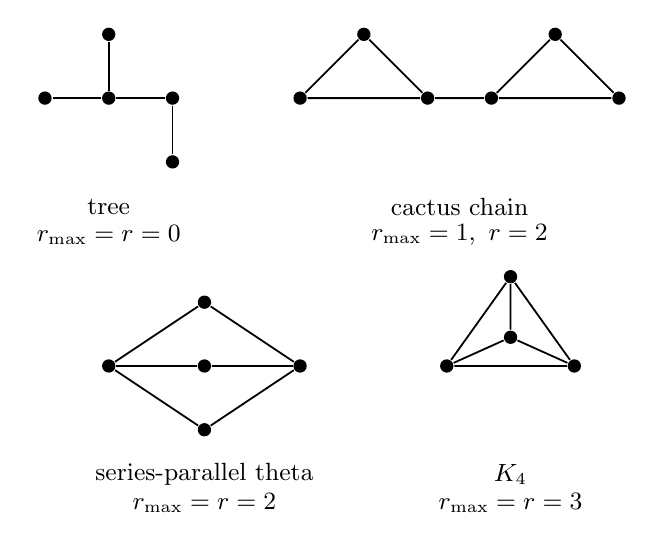
\begin{tikzpicture}[scale=.81, every node/.style={font=\small},
 vertex/.style={circle,fill,inner sep=1.7pt},line width=.65pt]
\begin{scope}
\foreach \n/\x/\y in {a/0/0,b/1/0,c/2/0,d/1/1,e/2/-1}
 \node[vertex] (\n) at (\x,\y) {};
\draw (a)--(b)--(c)--(e) (b)--(d);
\node at (1,-1.7) {tree};
\node at (1,-2.15) {$r_{\max}=r=0$};
\end{scope}
\begin{scope}[xshift=4cm]
\foreach \n/\x/\y in {a/0/0,b/1/1,c/2/0,d/3/0,e/4/1,f/5/0}
 \node[vertex] (\n) at (\x,\y) {};
\draw (a)--(b)--(c)--(a) (c)--(d) (d)--(e)--(f)--(d);
\node at (2.5,-1.7) {cactus chain};
\node at (2.5,-2.15) {$r_{\max}=1,\ r=2$};
\end{scope}
\begin{scope}[xshift=1cm,yshift=-4.2cm]
\node[vertex] (s) at (0,0) {};
\node[vertex] (t) at (3,0) {};
\foreach \i/\y in {1/-1,2/0,3/1}{
 \node[vertex] (v\i) at (1.5,\y) {};
 \draw (s)--(v\i)--(t);}
\node at (1.5,-1.7) {series-parallel theta};
\node at (1.5,-2.15) {$r_{\max}=r=2$};
\end{scope}
\begin{scope}[xshift=6.3cm,yshift=-4.2cm]
\foreach \n/\x/\y in {a/0/0,b/2/0,c/1/1.4,d/1/.45}
 \node[vertex] (\n) at (\x,\y) {};
\draw (a)--(b)--(c)--(a) (d)--(a) (d)--(b) (d)--(c);
\node at (1,-1.7) {$K_4$};
\node at (1,-2.15) {$r_{\max}=r=3$};
\end{scope}
\end{tikzpicture}
\caption{Four graph structures used in the complexity boundaries.
Adding cactus blocks raises total rank without raising maximum block
rank. Adding parallel paths inside one block raises both. The displayed
$K_4$ is the obstruction to universal individual-arc hull equality.}
\label{fig:main-topologies}
\end{figure}

Deleting a block's edges leaves components attached at its vertices.
Summing their nominations gives the block's effective nomination, and
the block's state depends only on that aggregate and its own laws.
Since the block--vertex incidence graph is a tree, a terminal difference
is the sum of drops along its unique block path, while an individual
arc belongs to one block. \Cref{lem:a-pre-block,lem:a-pre-incidence}
prove these facts without assumptions on flow signs. They are why
pressure and arc objectives have different exact-output guarantees.

\section{Localizing nomination uncertainty and separating arithmetic}
\label{sec:main-localization}

\begin{theorem}[Block-rank pressure and arc algorithms]
\label{thm:main-block}
Fix $r_0$. Let $G$ be connected with $r_{\max}\le r_0$, and let
nominations range over a nonempty balanced rational box.
For symmetric quadratic laws with independent positive rational
resistance intervals, every prescribed terminal-drop maximum satisfies
\eqref{eq:main-contract} in time polynomial in $N_\eps$ for fixed $r_0$.
Every individual arc has exactly computable algebraic minimum and
maximum of polynomial encoding length, so unfiltered robust signed
capacity validation is polynomial-time, including equality.

The same conclusions hold for laws affine in arbitrarily many independent
rational interval parameters, with densely encoded rational continuous
piecewise-polynomial basis functions vanishing at zero and fixed rational
breakpoints, provided every allowed complete law is strictly increasing.
Degrees and piece counts may grow. The pressure scenario output is
rational; the exact arc conclusion asserts algebraic values, without a
general rational near-extremal arc-output guarantee for these laws.
No additional operating bounds filter the nomination or coefficient
scenario domain in either assertion.
\end{theorem}

This combines \cref{thm:a-blk-joint,thm:a-blk-arc,thm:a-law-polynomial}.
For the independent affine-box representation, the dense-law
admissibility conditions can themselves be checked in polynomial time
(\cref{prop:a-law-validation}). The exponent depends on $r_0$ (an XP
bound); implicit laws and sparse binary exponents are not covered. By
\cref{prop:a-blk-limits}, based on
\citet{thurauf2022-deciding-the-feasibility-of-a}, block rank cannot be
replaced by treewidth two, series-parallel structure, or feedback vertex
number one unless $\mathrm P=\NP$, even with fixed resistances.

\subsection{Proof mechanism: adjoint levels and small faces}

The first reduction removes components outside the terminal block path
and sums their nomination intervals at the attachment vertices. Every
feasible aggregate has a rational disaggregation, obtained by filling
the original intervals from their lower bounds. Since the domain is
unfiltered, no operating constraint is lost.

Temporarily smooth the edge laws so their derivatives are positive.
Differentiating \eqref{eq:main-state} and pairing with the terminal
objective gives
\begin{equation}
 dF_{s,t}=h^\top db,\qquad
 A\operatorname{diag}(1/g'_e(x_e))A^\top h=e_s-e_t.
 \label{eq:main-adjoint}
\end{equation}
The adjoint $h$ is the potential of a unit electrical network. At a
maximum over a balanced box, a multiplier $\mu$ for balance exists such
that $h_v>\mu$ forces $b_v=u_v$ and $h_v<\mu$ forces $b_v=\ell_v$, so
only nominations at the level $h_v=\mu$ remain free. The maximum
principle strictly orders the adjoint ranges of consecutive blocks, so
one threshold meets internal vertices of at most one block.

On a cactus, the adjoint is strictly monotone down each of the two
branches of that block. At most two nominations remain free, one on
each branch, and balance leaves one parameter; there are $O(n^2)$
candidate faces. On a higher-rank block, mark the terminals and the
vertices of degree at least three, and suppress the degree-two paths
between them; there are at most $2r_B$ marks and $3r_B-1$ paths. A small
positive objective source at every unmarked vertex makes the electrical
current strictly increase along each path, so its potential is unimodal
and every threshold occurs at most twice. Enumerating the resulting
lower/free/upper/free/lower patterns leaves at most $8r_B-2$ free
nominations. Compactness and uniform convergence remove the smoothing
and perturbation; the algorithm enumerates closed faces and never
computes a perturbation size.

\begin{figure}[tb]
\centering
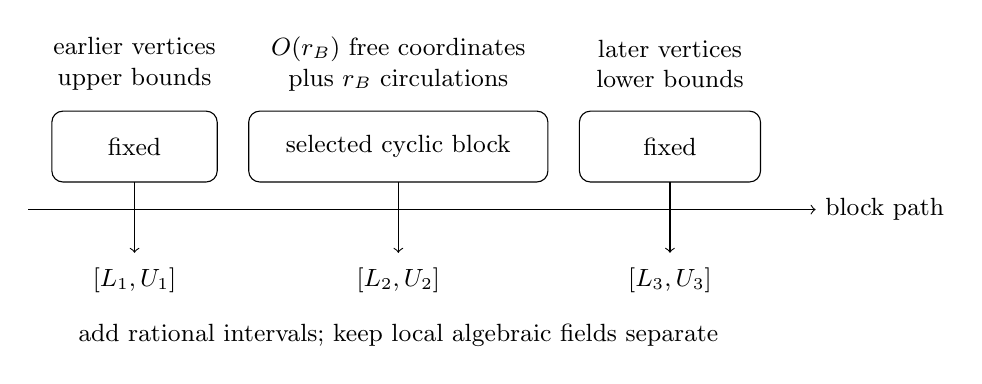
\begin{tikzpicture}[x=1cm,y=1cm,every node/.style={font=\small}]
\draw[->] (0,0)--(10,0) node[right] {block path};
\foreach \a/\b/\txt in {0.3/2.4/fixed,2.8/6.6/selected cyclic block,7/9.3/fixed}{
 \draw[rounded corners] (\a,.35) rectangle (\b,1.25);
 \node at ({(\a+\b)/2},.8) {\txt};}
\node[align=center] at (1.35,1.85) {earlier vertices\\upper bounds};
\node[align=center] at (4.7,1.85) {$O(r_B)$ free coordinates\\plus $r_B$ circulations};
\node[align=center] at (8.15,1.85) {later vertices\\lower bounds};
\draw[->] (1.35,.35)--(1.35,-.55);
\draw[->] (4.7,.35)--(4.7,-.55);
\draw[->] (8.15,.35)--(8.15,-.55);
\node at (1.35,-.9) {$[L_1,U_1]$};
\node at (4.7,-.9) {$[L_2,U_2]$};
\node at (8.15,-.9) {$[L_3,U_3]$};
\node at (4.7,-1.6) {add rational intervals; keep local algebraic fields separate};
\end{tikzpicture}
\caption{Nomination localization for a terminal difference. Independent
coefficients may still be optimized in every block; ``fixed'' refers to
aggregated nominations. The selected block is cyclic; bridge cases
are handled directly. The number of blocks is unrestricted.}
\label{fig:main-localization}
\end{figure}

The second reduction handles the many coefficient variables. Inside
a selected face, flow is affine in the free nominations and the
$r_B$ cycle circulations. On each flow-sign or law-piece cell, the
cycle equations are polynomial in this small core and affine in the
coefficient parameters, so the image of a coefficient box in the cycle
and objective coordinates is a zonotope of fixed dimension. Its support
inequalities can be expanded over the realizable sign patterns, which
are polynomially many at fixed dimension, and quantifier elimination
removes the remaining fixed-dimensional support variables. The leaf
coordinates are recovered from exposed zonotope vertices and a
fixed-size convex combination. This avoids enumerating all box corners;
the fact that an LP vertex has few non-bound coordinates would not by
itself give an efficient algorithm.

The fixed-dimension bounds are classical
\citep{renegar1992-on-the-computational-complexity-and,basu2006-algorithms-in-real-algebraic-geometry};
we keep the number of real variables bounded \emph{per block}, even
when law degrees and numbers of uncertain coefficients grow. Independent
block optima are enclosed separately and their rational intervals added.
A pressure sensitivity estimate then permits rational rounding inside
the original nomination and coefficient constraints. The proofs in
\cref{sec:a-block-rank,sec:a-laws} handle ties, zero flows, singleton
faces, degenerate polytopes, and output bit length.

\subsection{An exact arithmetic boundary on a chain of triangles}

\begin{theorem}[Cactus arithmetic and fixed fractional powers]
\label{thm:main-arithmetic}
For symmetric quadratic laws with fixed positive rational resistances,
MPD over a balanced rational nomination box on a cactus satisfies
\eqref{eq:main-contract} in polynomial time. On the restricted box
$b=\zeta(e_s-e_t)$, $0\le\zeta\le1$, exact weak threshold comparison
is polynomial-time many-one equivalent to Square-Root Sum. Hardness
holds on simple degree-three chains of triangles with positive integer
resistances.

For every fixed finite family $\mathcal Q\subset\Q\cap(1,\infty)$,
the laws $g_e(t)=\beta_e\sgn(t)|t|^{q_e}$, $q_e\in\mathcal Q$, admit
the additive value and rational-scenario contract for terminal drops
and individual arcs at fixed maximum block rank, over a balanced rational
nomination box and independent positive rational resistance intervals,
without operating filters. For any fixed reduced exponent greater than
one with even denominator, exact arc-capacity comparison is
Square-Root-Sum hard already on a single simple cycle with fixed integral
nominations and positive integral resistances.
\end{theorem}

The quadratic statements are \cref{thm:a-cac-additive,thm:a-cac-srs};
the power-law statements are \cref{thm:a-law-fractional,thm:a-law-srs}.
Square-Root Sum asks whether $\sum_i\sqrt{a_i}\le K$ for positive
binary integers $a_i,K$. Whether it is decidable in polynomial time, or
even lies in NP, is open (see also \citet[Section 5]{ajdarow2025-taming});
its known upper bounds are discussed in \cref{subsec:a-pre-computation}.

The arithmetic gadget uses a triangle whose two terminal branches have
total resistances $(a-1)^2$ and $(a-1)^2/a$ for $a\ge2$. Its unit-flow
drop is
\[
 R_a=a+1-2\sqrt a>0.
\]
Joining these triangles by unit bridges produces
$\Delta=C-2\sum_i\sqrt{a_i}$, and scaling by a positive common
denominator makes every resistance integral without changing the weak
comparison. Conversely, each unloaded cycle on a unit source-to-sink
cactus contributes a rational number minus one positive radical, so
their sum reduces to Square-Root Sum. Multiple-entry cycles have
different local formulas, so this converse is not asserted for arbitrary
nomination boxes. An existential-real formulation gives the general
upper bound $\ETR\subseteq\PSPACE$ for exact quadratic MPD
(\cref{prop:a-cac-etr}).

For fractional powers, the monotone loop equation of one cycle can
encode the radical sum directly at a rational circulation threshold.
Additive algorithms avoid this exact comparison by using positive
rational approximations to the laws. Positive quadrature fractions,
with a fixed odd-power factor when necessary, preserve strict
monotonicity and have a dense encoding polynomial in accuracy bits, and
an explicit monotonicity estimate transfers constitutive error to flow
and potential error. This adds network and parameter-recovery guarantees
to established fractional-power approximation
\citep{bonito2015-numerical-approximation-of-fractional-powers} and
rigorous quadrature \citep{johansson2018-gauss-legendre}. The water
head-loss exponent $1.852=463/250$
\citep[Example 2.3]{gro2017-algorithmic-results-for-potential-based}
falls under both parts of the theorem.

\section{The observable determines the topology boundary}
\label{sec:main-observables}

Replacing finite resistance sets by their interval hulls is attractive,
since continuous coefficients can be eliminated through convex images,
whereas a product of finite sets has exponentially many choices. Whether
the replacement preserves an extremum depends on the graph \emph{and}
the objective. In this section a universal statement
quantifies over every fixed balanced nomination and all independent
compact positive resistance sets with attained endpoints, under quadratic
laws and without operating filters.

\begin{theorem}[Universal resistance-hull and region classifications]
\label{thm:main-hulls}
For finite connected simple graphs, the universal interval-hull classes
for maxima and minima are exactly those in \cref{tab:main-hulls}.
The same classes characterize separate monotonicity in every resistance
coordinate, with the other coordinates fixed. The attainable flow region
is convex for every fixed nomination and positive resistance box exactly
on cacti. Normalized potential regions and joint flow--potential regions
are universally convex exactly on trees.
\end{theorem}

\begin{table}[tb]
\centering\small
\begin{tabularx}{\linewidth}{@{}Yl@{}}
\toprule
Observable whose extrema must be preserved & Universal graph class\\
\midrule
Every balanced weighted potential $c^\top\pi$ & Trees\\
Every prescribed difference $\pi_s-\pi_t$ & Cacti\\
Every linear flow objective $d^\top x$ & Cacti\\
Every individual arc flow $x_a$ & Series-parallel\\
\bottomrule
\end{tabularx}
\caption{Exact equality of resistance-set and interval-hull extrema
under fixed nominations, independent compact positive quadratic
resistance sets, and no operating filters. Equality of extrema does not
assert an exact scalar comparison algorithm.}
\label{tab:main-hulls}
\end{table}

These claims are \cref{thm:a-weight-hierarchy,thm:a-weight-convex-regions},
with the individual-arc equivalence proved in
\cref{thm:a-bound-characterization}. Counterexamples use rational data,
one varying resistance, and strictly positive resistances on all other
edges. The full-region
classifications extend qualitatively to every fixed common power
$\sgn(x)|x|^q$ with $q>0$, $q\ne1$, without a uniform bit bound or
algorithm (\cref{thm:a-weight-power-regions}). With linear laws, by
contrast, every graph has the hull property for potential objectives
(\cref{sec:a-weighted}).

\subsection{Finite comparison and deterministic envelopes}

A finite secant argument explains the positive individual-arc result
without differentiating a law at zero. The difference of two passive
states for the same nomination and two law profiles is an electrical
network with positive secant resistances and explicit edge disturbances.
For a target edge $a=(u,v)$, let $j$ be the unit electrical current from
$u$ to $v$ in that secant network. The target flow difference is a
linear combination of the disturbances, with coefficients $j_e$ for
$e\ne a$ and $-(1-j_a)$ on $a$, divided by the positive target secant
resistance. By classical confluence, the signs of these currents do not
depend on the positive resistances when the graph is series-parallel.

One may therefore select, pointwise in flow, a maximum or minimum
allowed law on each edge according to the sign of its current $j_e$. The target
state of the resulting deterministic envelope attains the uncertainty
extremum, and compactness makes the selected law value realizable by an
original parameter at that state. The construction is uniform in the
nomination, although the realizing profile can depend on the state
(\cref{thm:a-bound-envelope-structural}, for independent compact
continuous law families). For quadratic interval or finite resistance
uncertainty the envelope is directional quadratic, and its primitive
has a linear-size second-order-cone formulation. Rational convex
optimization and recovery then give polynomial additive arc optimization
for fixed nominations on every series-parallel graph, without a rank
bound (\cref{thm:a-bound-envelope-algorithm}).

Deterministic feasibility for rated monotone characteristics has related
series/parallel propagation methods: Zemanian's report uses endpoint
propagation and operating-point recovery
\citep[Conditions 2.1, Lemmas 4.1 and 5.1, Procedure 8.1]{zemanian1999-ratings}.
Those deterministic procedures do not provide the present
uncertainty-envelope and accuracy-bit output guarantees.

\subsection{What fails when the objective changes}

A triangle already separates weighted potentials from pairwise
potentials. With edges oriented $0\to1\to2\to0$, resistances
$(1,1,\theta)$, nominations $(2,-3,1)$, and
$c=(-5,12,-7)$, the circulation $q$ satisfies
$6q+3-\theta q^2=0$ on $-1/2<q<0$. Its weighted potential is
\[
 W=-\frac{105}{4}-12(q+1/4)^2.
\]
At $\theta=24$, $q=-1/4$ and $W=-105/4$. At
$\theta=16/3$ and $144$, the circulation is respectively $-3/8$ and
$-1/8$ and both values are smaller by $3/16$. Thus a two-point set
and its interval hull give different weighted-potential optima on one
cycle, although this graph is in the universal class for every
individual potential difference. Weighted cancellation changes the
extremal geometry.

A rank-two theta block supplies the corresponding linear-flow
counterexample; a rank-three $K_4$ supplies the individual-arc
counterexample. Subdividing suitable uncertain paths encodes Subset
Sum at the same small block rank, giving the discrete boundaries in
\cref{tab:main-boundaries}, with explicit rational gaps and positive
integer resistances where stated. Multiplying all resistances scales a
pressure gap but leaves flows unchanged; flow gaps are amplified by
scaling nominations instead.

\begin{table}[tb]
\centering\small
\begin{tabularx}{\linewidth}{@{}P{.22\linewidth}P{.26\linewidth}Y@{}}
\toprule
Objective and graph & Scenario assumptions & Computational conclusion\\
\midrule
Potential difference; one rank-two block & Fixed small nominations;
independent two-point resistances & NP-hard, with polynomial-bit gap
(\cref{thm:a-bound-pressure}).\\[3pt]
Individual arc; series-parallel, fixed block rank & Balanced nomination
box; independent finite resistances & Exact algebraic extrema and robust
capacity decision; includes every rank-at-most-two graph
(\cref{cor:a-bound-finite-positive}).\\[3pt]
Individual arc; rank-three block & Fixed small nominations;
independent two-point resistances & Existential strict or weak threshold
is NP-complete; complementary universal test is coNP-complete
(\cref{thm:a-bound-arc-hardness}).\\[3pt]
Weighted potential; one cycle & Fixed nominations and three objective
support vertices; independent finite resistances & NP-complete threshold
attainment, coNP-complete robust upper bounds
(\cref{thm:a-weight-cycle-hard}).\\[3pt]
Linear flow; rank-two block & Fixed nominations; independent finite
resistances & NP-complete threshold attainment; includes unit-cost total
absolute flow on a DAG (\cref{thm:a-weight-flow-hard}).\\[3pt]
Individual arc; series-parallel with growing block rank & Balanced
nomination box; fixed resistances & NP-hard optimization and coNP-hard
robust upper bounds; no general membership claim
(\cref{thm:a-bound-nomination}).\\
\bottomrule
\end{tabularx}
\caption{Discrete and nomination boundaries for quadratic laws. All
rows use unfiltered scenarios. Hardness gaps obstruct polynomial
accuracy-bit algorithms unless P equals NP; they are not uniformly
strong-hardness claims.}
\label{tab:main-boundaries}
\end{table}

Two further distinctions matter. First, the envelope theorem and hull
equality do not settle exact scalar arithmetic on unrestricted
series-parallel graphs. A parallel probe on a cactus branch transfers its radical sum
to an arc comparison, giving Square-Root-Sum hardness even with fixed
unit nominations and fixed integral resistances; a restricted probe
family has the converse reduction (\cref{thm:a-bound-arc-srs}). Second,
hull preservation for an extremum does not preserve exact realization
of a target flow. For a prescribed rational $\bar x$, conservation can
be checked and the equations $A^\top\pi=(\beta_e\bar x_e|\bar x_e|)_e$
are linear in $\pi,\beta$, so interval realization is an LP on any
graph. With two finite resistance choices per uncertain edge it is
NP-complete on one simple cycle, and so is existential unit-capacity
design on that cycle (\cref{thm:a-bound-realization}). These are
existential questions, whereas robust validation tests every scenario.

\section{Weighted objectives and many interacting block responses}
\label{sec:main-weighted}

A terminal difference is a weighted potential with two nonzero
coefficients. General weights can create competing local contributions,
so one-active-block localization no longer suffices. This is an actual
complexity issue, not just a limitation of the proof: with growing
objective support, weighted-potential threshold attainment is
NP-complete on degree-three trees with fixed resistances and a balanced
nomination box. The reduction also excludes absolute-error $1/8$
approximation on its unnormalized family. At fixed support $p$, trees
instead admit exact rational extrema, scenarios, flows, and potentials
in $N^{O(p)}$ time (\cref{thm:a-weight-tree-hard,thm:a-weight-tree-algorithm}).

\subsection{Three completed weighted extensions}

\begin{theorem}[Weighted accuracy-bit algorithms]
\label{thm:main-weighted}
Let $W=c^\top\pi$ with $c\in\Q^V$ and $\one^\top c=0$. Consider any of:
fixed positive rational asymmetric quadratic coefficients; independent positive rational
symmetric coefficient intervals; or independent positive rational
directional coefficient intervals. Scenarios have no operating filters.
In each of the following cases, both extrema satisfy the rational
value and original-scenario contract \eqref{eq:main-contract} in time
polynomial in $N_\eps$ for the fixed parameters:
\begin{enumerate}
\item The graph is a cactus. Nominations form a rational balanced affine
family on a nonempty compact rational polytope of fixed dimension $d$; objective
support and total cycle rank are unrestricted. Alternatively, nominations
range over a balanced rational box and $p=|\supp c|$ is fixed.
\item Maximum block rank is at most a fixed $r_0$, and nominations
range on one nonempty compact rational affine line segment. Objective
support, number of noncactus blocks, and total cycle rank are unrestricted.
\item Put $\kappa(G)=\sum_{B:r_B\ge2}r_B$. The total noncactus rank
$\kappa(G)$ is bounded by a fixed $\kappa_0$, and the balanced affine
nomination domain has fixed dimension $d$. Alternatively, use a balanced
rational nomination box and fixed objective support $p$. Cactus rank
is unrestricted.
\end{enumerate}
In case 2 with fixed laws, the conclusion also holds for admissible
densely encoded rational continuous piecewise-polynomial laws vanishing
at zero, with fixed rational breakpoints and growing degrees and piece
counts. That extension returns rational nominations and does not assert
uncertain polynomial coefficients.
\end{theorem}

Case 1 is \cref{thm:a-wcac-affine,cor:a-wcac-box}; case 2 is
\cref{thm:a-wblk-line,cor:a-wblk-line-polynomial}; case 3 is
\cref{thm:a-wblk-hybrid,cor:a-wblk-hybrid-box}.
For comparison, fixed \emph{global} cycle rank $r$ and fixed support
$p$ permit exact algebraic weighted extrema and algebraic scenarios
under independent continuous resistance intervals
(\cref{thm:a-weight-global}). There all nonlinear variables fit in one
common algebraic field. Fixed rank per block allows an unbounded number
of independent fields, so it requires the separate summation arguments.

The graph and support parameters can sometimes be reduced further.
On a tree, contract every edge with zero induced objective cut flow,
then orient each remaining edge along positive cut flow. Only vertices
that fail to have exactly one incoming and one outgoing edge need be
marked. If their number $k$ is fixed, exact optimization takes $N^{O(k)}$
time even with growing support. At fixed global rank a supplied marked
set and constant source sign on each suppressed path give a related
signed-path refinement, including returning paths. These statements
are formalized in \cref{thm:a-weight-tree-algorithm,thm:a-weight-global};
they describe checkable structural information, not an assumption that
all objective weights have the same sign.

\subsection{A face theorem and two ways to sum}

Choose a rational tree flow $w$ satisfying $Aw=c$. Then
\[
 W=c^\top\pi=w^\top A^\top\pi=\sum_e w_eg_e(x_e).
\]
This puts each contribution in its physical block. Prune subtrees with
no objective support and contract a block if every induced objective
sum at its attachments vanishes. Both operations preserve the objective
and admit rational nomination disaggregation. The incidence subtree
spanning $p$ objective vertices has only $O(p)$ branching locations
and ordinary chains. An adjoint threshold can leave one selected block
per ordinary chain plus the special blocks. Path suppression and a
second positive-source perturbation then leave $O(r_0p)$ free nominations
on $n^{O(r_0p)}$ closed faces for a positive bound $r_0\ge1$ with
$r_{\max}\le r_0$ (\cref{thm:a-wcac-faces}). This full weighted
face reduction is independent of the coefficients. It is structural;
it does not imply an additive algorithm for an arbitrary number of
higher-block value functions of several parameters.

For a quadratic cactus, a local circulation equation is piecewise
quadratic. With uncertain coefficients, a single equality LP first
eliminates the resistance choices. Reduced costs are ordered by one
weight threshold; tied weights remain as a recoverable interval sum.
The complete circulation candidates include boundaries, stationary
points, flat pieces, and zero-flow cases. A local maximum is therefore
selected from polynomially many rational or quadratic-radical formulas
in the nomination parameters. Geometrically spaced rational polynomial
panels approximate the square roots, and a common sign decomposition
allows all block surrogates to be added in the \emph{same} fixed-dimensional
nomination coordinates. Exact optimization of the surrogate uses a
fixed number of variables; it does not introduce one value variable
for every cycle. Global continuity then recovers original rational
parameters, even if rounding changes local flow signs.

For higher-rank blocks on one nomination line, local algebraic degree
need not be two. The key interface becomes a rational quantifier-free
graph of a scalar Lipschitz semialgebraic function. The construction in
\cref{lem:a-wblk-univariate} isolates exceptional parameters, uses the
Lipschitz bound on small neighborhoods, and constructs rational analytic
interpolants on geometric panels elsewhere. Polynomial dependence on
dense degree, coefficient bits, and accuracy bits is proved explicitly.
The resulting rational polynomials retain the original parameter $t$,
so arbitrarily many block responses can be added and optimized without
forming their joint algebraic field. This is why the one-line result
can allow an unrestricted number of higher-rank blocks.

For several nomination parameters, case 3 instead keeps all noncactus
circulations in one exact core of dimension $d+\kappa(G)$ and compiles
the remaining cactus contributions. The quantity $\kappa(G)$ is a
\emph{sum}, not a maximum. A graph with a thousand rank-two blocks
does not have small $\kappa(G)$ merely because each block has rank two.
The separate one-line theorem does apply to that graph.

\subsection{Exact parameters, filters, and limits}

At fixed rational nominations on a cactus, the quadratic weighted
algorithm gives an exactly optimizing rational coefficient profile,
even with optional signed arc capacities and arbitrary objective support.
Its local values have degree at most two, and the global value may be
retained as their separate sum (\cref{thm:a-wcac-exact-profile}).
An exact profile need not be an endpoint profile: on the four-cycle in
\cref{ex:a-wcac-interior}, the unique optimum is $(1,2,1,1)$ and the
second coefficient lies strictly inside $[1,3]$.
Thus a polynomial exact scenario output is compatible both with an
interior optimum and with the absence of an efficient exact scalar
comparator for its value.

For fixed-dimensional affine nominations, local capacity filters permit
exact feasibility and additive algebraic scenarios of polynomial
representation size. With fixed laws, closed bounded-degree
semialgebraic filters involving the nomination parameters and one block's
flows are also allowed. The joint coefficient theorem permits only the
stated affine arc bounds. A supplied positive tightening margin gives
a rational scenario feasible for the original capacities and near-optimal
relative to the \emph{tightened} optimum
(\cref{thm:a-wcac-capacities}). The reference optimum matters: a small
coefficient perturbation need not preserve an optimizer lying on an
exact capacity boundary.

Indeed rational inputs can force an irrational nomination. The four-cycle
in \cref{ex:a-wcac-irrational} has flows
$(q+t-1,q-2,q,q-2)$ and resistances $(1,1,1,2)$.
The bounds $|x_3|\le1$ and $|x_4|\le1$ force $q=1$; the
cycle equation becomes $t^2=2$ for $1\le t\le2$.
Thus no rational feasible nomination exists. This is an output
obstruction, not a contradiction to the unfiltered rational approximation
theorems.

The unresolved weighted case is now specific: several fixed shared
nomination parameters, an unrestricted number of higher-rank blocks,
and only a fixed \emph{maximum} block rank. The local value graphs and
face reduction are available. What remains outside the proved algorithms
is accuracy-bit optimization of their growing sum in the original
shared coordinates (\cref{eq:a-wblk-residual}). A Lipschitz grid is
polynomial in $1/\eps$, and retaining all local values defeats
fixed-dimensional elimination. These observations delimit those methods;
they are not a hardness or impossibility result.

\section{Continuous design, correlations, and the direction of optimization}
\label{sec:main-design}

With fixed nominations, every cactus cycle has one scalar circulation.
This permits considerably more coefficient dependence than the independent
edge boxes used in nomination optimization. It also exposes a boundary
between correlations within a cycle and correlations across cycles.

For each edge let
$g_e(x;\theta)=g_{e0}(x)+\sum_j\theta_jg_{ej}(x)$,
with densely encoded rational polynomial pieces, fixed rational
breakpoints, and admissible continuous strictly increasing complete
laws vanishing at zero throughout the parameter domain. The degree,
number of pieces, and parameter dimension may grow. Admissibility is
a promise in this correlated model. Bridge flows are fixed by the
nomination; a consistently oriented cycle has
$x_e=x_e^0+\chi_eq$ and loop equation
\[
 H_C(q,\theta)=\sum_{e\in C}\chi_eg_e(x_e^0+\chi_eq;\theta)=0.
\]
This function is continuous, strictly increasing in $q$, and affine
in $\theta$. Rational bounds on total injection supply a root bracket.

\begin{theorem}[Cycle-local design and global capacity recovery]
\label{thm:main-design}
Let $G$ be a connected simple cactus with fixed rational balanced
nominations and the admissible affine polynomial-law model above.
\begin{enumerate}
\item If each cycle has its own independent nonempty bounded rational
parameter polytope, the attainable flow region is
$x=x^0+Zq$ with independent algebraic circulation intervals.
Rational cycle-local signed capacities clip these intervals exactly.
Feasibility, each interval endpoint, and a rational original parameter
profile attaining it are computable in polynomial bit time. Linear
flow objectives admit exactly optimizing rational profiles and additive
scalar values, with no exact-comparison claim for a growing sum.
\item In the same independent-cycle model with those capacities, a
densely encoded rational polynomial flow objective promised convex on
$[-B-1,B+1]^m$, $B=\sum_v|b_v|$, admits an exactly feasible rational
parameter scenario within $\eps$ of its minimum in polynomial
accuracy-bit time. Degrees and number of cycles are unrestricted.
For maximization of $g(Rx)$, the analogous additive scenario guarantee
holds when $R\in\Q^{k\times m}$ has fixed row count $k$ and the dense
rational polynomial $g$ is convex on a box containing the attainable
measurements.
\item If one nonempty bounded rational parameter polytope instead
couples all cycles, feasibility of signed arc capacities is rational
linear feasibility and has a rational witness. Robust capacity testing
uses rational LPs and returns rational violating profiles when needed.
Individual arcs have exact algebraic extrema and rational optimizing
profiles, including when other such capacities filter the domain.
\end{enumerate}
All complexity bounds count dense input and output bits. These statements
exclude variable nominations and potential filters; part 2 excludes
flow constraints coupling distinct cycle coordinates.
\end{theorem}

These are \cref{thm:a-design-independent,thm:a-design-convex,thm:a-design-measurements,thm:a-design-global-capacity}.
The few-measurement maximization conclusion also holds for independent
finite quadratic resistance sets at fixed nominations, without capacity
filters. Its dependence is $N^{O(k)}$ times a polynomial in accuracy
bits, and it promises a near-optimal scenario rather than exact
comparison of candidate values. A positive-semidefinite quadratic of
fixed rank $r$ uses at most $r+1$ measurements, including its linear
term (\cref{cor:a-design-fixed-rank}).

\subsection{Why scalar roots admit exact rational parameter recovery}

At a rational $z$, strict increase gives
\[
 \max_{\theta\in P}q(\theta)\ge z
 \quad\Longleftrightarrow\quad
 \min_{\theta\in P}H_C(z,\theta)\le0.
\]
The right side is an LP, regardless of the parameter dimension.
A largest root is attained at a vertex of $P$: expressing any profile
as a convex combination of vertices expresses its zero loop value as
the same combination, so at least one vertex has a root no smaller.
Vertex coordinates have polynomial bit bounds from determinants.
After substitution, all vertex-piece roots therefore satisfy a common
degree and coefficient-height bound. Root separation gives a polynomial
number of bisection bits sufficient to distinguish unequal candidate
roots, without enumerating vertices. An LP vertex at the final threshold
must attain the exact extreme root. \Cref{thm:a-design-root} proves this
step for general monotone dense piecewise-polynomial root families,
including repeated roots, breakpoint roots, and lower-dimensional
polytopes.

Capacities are equally direct. A lower bound $q\ge a$ is equivalent
to $H_C(a,\theta)\le0$, and an upper bound $q\le b$ is equivalent
to $H_C(b,\theta)\ge0$. Both are linear in the original parameters.
This remains true under global correlations. Independence across cycles
is needed only to combine the scalar attainable intervals into a box.
A rational circulation target can be realized by another rational LP.
Together with exact endpoint profiles, this permits recovery even when
a clipped interval is an irrational singleton.

Dense convex minimization uses rational inner boxes approximating the
algebraic circulation box, a controlled convex extension for a polynomial
promised convex only on the stated cube, and exact rational oracles.
The optimizer is mapped back to original coefficients with exact
capacity feasibility. For convex maximization through $k$ measurements,
the circulation box projects to a zonotope. Rational generator directions
determine a polynomial number of exposed candidates at fixed $k$.
Their algebraic values are compared approximately and their endpoint
profiles recovered separately. This is the network application of the
classical zonotope approach, with the irrational endpoint and accuracy
accounting made explicit.

\subsection{Independence and convexity do not make every objective easy}

Independent coefficient intervals can realize a circulation cube on a
bounded-data cactus. A coupled convex quadratic on that cube encodes
Max-Cut. Thus convex maximization in all flows is strongly NP-hard,
even with unit terminal nominations, maximum degree three, and resistances
in $[1,16]$; absolute-error $1/4$ approximation remains hard
(\cref{thm:a-design-maxcut}). The positive fixed-measurement theorem
restricts the dimension of the measured image, not merely the degree
or convexity of the objective.

Global correlations can destroy even linear-flow tractability. Two
cycles sharing one resistance already have a curved attainable image:
in \cref{ex:a-corr-shared}, two selected flows satisfy
$x_2=2x_1/(1+x_1)$ on $1/3\le x_1\le1/2$.
Their difference has its strict maximum at the interior shared
resistance $\theta=2$, although its two endpoint values agree. This
example alone proves no hardness, but explains why independent-cycle
endpoint reasoning cannot be reused. A separate paired-triangle
construction proves strong hardness for total-flow maximization and
minimum dissipation over a global resistance polytope, with all
resistances in $[1,3]$, positive flows, and a fixed absolute gap
(\cref{thm:a-corr-hardness}).

For symmetric quadratic laws write
\[
 D(\beta)=b^\top\pi(\beta)=\sum_e\beta_e|x_e(\beta)|^3
          =3\min_{Ax=b}\sum_e\beta_e|x_e|^3/3.
\]
This is constitutive dissipation; the primitive energy is $D/3$ at the
physical state. As a pointwise infimum of linear functions of $\beta$,
$D$ is concave. The direction of optimization is therefore decisive.

\begin{theorem}[Maximum dissipation over a global polytope]
\label{thm:main-energy}
On any connected graph with fixed rational balanced nominations and
symmetric quadratic laws, let resistances range over a nonempty bounded
rational polytope with supplied positive rational lower and upper bounds.
Maximum physical dissipation has an exact formulation with two
second-order cones per edge and a rational admissible profile within
$\eps$ of its maximum computable in polynomial accuracy-bit time.
No operating filters are imposed. On a cactus, rational signed arc
capacities may be added: infeasibility is decided, or the same guarantee
holds with every original capacity satisfied exactly.
\end{theorem}

This is \cref{thm:a-corr-energy-max,cor:a-corr-energy-capacity}.
Cubic energy duality is classical; for the symmetric network model it
is already developed in
\citet{gro2017-algorithmic-results-for-potential-based}.
The contribution here includes the global resistance-polytope formulation,
explicit rational output and precision argument, and original-instance
certificate in \cref{prop:a-corr-certificate}. Concavity of effective
resistance also has classical linear-network precedent
\citep{shannon1956-concavity}. Neither this mechanism nor the theorem
extends by assertion to arbitrary potential filters.

\subsection{Rational witnesses need margins beyond the scalar setting}

Exact capacities beyond cacti can force irrational coefficients even
when every capacity is an ordinary positive-width upper bound. A simple
rank-two series-parallel instance with one uncertain resistance gives
such an example (\cref{prop:a-corr-irrational}). Thus rational feasibility
on a cactus reflects the scalar loop equation, rather than a general
property of rational physical models.

Strict slack restores a quantitative rational witness statement on
any graph. For fixed nonzero nominations put $M=\tfrac12\|b\|_1$.
If two symmetric or directional coefficient profiles have lower bound
$\beta_L>0$, and $q_e$ is the absolute symmetric coefficient change
or the larger of the two directional changes on edge $e$, then
\begin{equation}
 \|x'-x\|_\infty\le\frac{M}{2\beta_L}\sum_e q_e.
 \label{eq:main-sensitivity}
\end{equation}
\Cref{prop:a-corr-sharper} proves this bound through regularized
electrical sensitivity and a limiting argument, including zero flows
and reversals. It is four times smaller than the
uniform estimate in \cref{thm:a-corr-lipschitz}; optimality of its
constant is not claimed. A feasible real profile with supplied rational
capacity slack can consequently be rounded safely. The appendix also
extends witness-size recovery to a rational global coefficient polytope
by intersecting an isolating rational box with that polytope. This is a
conditional existence and rounding guarantee; it is not an algorithm
for locating the initial strictly feasible profile.

\section{Certificates for physical outputs and original scenarios}
\label{sec:main-certificates}

A numerical solution raises a question that the preceding algorithms do
not: what does its actual output prove? For a fixed directional
quadratic network with at least one edge, rational nominations, and
positive rational coefficients, rational witnesses answer this
independently of a solver's stopping rule and can be attached to a
verified uncertainty-envelope reduction.

Write
$E_e(t)=\beta_e^{\sgn(t)}|t|^3/3$ and $E=\sum_eE_e$,
where the positive coefficient is selected at zero by convention.
Let $x^*$ minimize $E$ on $Ax=b$, and let
$\beta_L=\min_{e,\sigma}\beta_e^\sigma>0$.
The statement below uses a connected graph for simplicity; the
appendix and the deterministic certificate verifiers also allow several
components with feasible nominations and separate gauges. The
original-envelope reader and the numerical conservation-repair producer
require a connected simple loopless graph.

\begin{theorem}[Rational energy and conserved-curvature certificates]
\label{thm:main-certificates}
Suppose $y\in\Q^m$ satisfies $Ay=b$, $p\in\Q^V$, and rational
$\zeta_e\ge0$ satisfy
$\zeta_e^2\beta_e^{\sgn((A^\top p)_e)}\ge|(A^\top p)_e|^3$.
Then
\[
 L=b^\top p-\tfrac23\sum_e\zeta_e\le E(x^*)\le E(y),
 \qquad \delta=E(y)-L\ge0.
\]
Every rational $\eta\ge0$ with $\beta_L\eta^3\ge6\delta$
certifies $\|x^*-y\|_\infty\le\eta$.

More generally, suppose verified rational intervals $[l_e,u_e]$
contain both $y_e$ and $x_e^*$. Set $h_e=2\beta_e^+l_e$ when
$l_e>0$, $h_e=-2\beta_e^-u_e$ when $u_e<0$, and $h_e=0$ otherwise.
For a rational linear goal $w$, let $v$ be rational and put
$s=w-A^\top v$. If $s_e=0$ wherever $h_e=0$, define
$C(v)=\sum_{h_e>0}s_e^2/h_e$. Every rational $r\ge0$ with
$r^2\ge2\delta C(v)$ certifies
$|w^\top(x^*-y)|\le r$.
The least factor $C_*$ is attained by rational linear algebra whenever
the zero-edge condition is feasible. For $\delta>0$,
$\sqrt{2\delta C_*}$ is the exact supremum of $|w^\top d|$ over
$Ad=0$, $\tfrac12\sum_e h_ed_e^2\le\delta$. If the zero-edge
condition is infeasible, that supremum is infinite. All displayed
witness conditions are checkable by rational arithmetic in polynomial
time in their encoded lengths.
\end{theorem}

The first assertion is \cref{prop:a-cert-energy}; the goal assertions
are \cref{thm:a-cert-hessian,prop:a-cert-projection}. Both require the
trial flow to be exactly conserved, $Ay=b$; a small conservation
residual cannot replace this. Sharpness refers to the \emph{conserved
quadratic error set} just stated, not to every physical error or to the
additional coordinate intervals. At zero gap, $x^*=y$ and all goals are
exact without a curvature condition.

\subsection{From energy to intervals and linear goals}

The scalar conjugate is
$E_e^*(d)=\tfrac23\sqrt{|d|^3/\beta_e^{\sgn(d)}}$.
Rational upper root bounds make the dual lower energy check exact, and
uniform cubic convexity converts the gap into a flow radius. This
specializes classical Fenchel duality and primal-dual error control
\citep{boyd2004-convex,bartels2020-primal-dual}.

Separate-edge bounds can be sharpened using the reverse Bregman
expression
\[
 D_e(y_e,z)=E_e(y_e)-E_e(z)-E'_e(z)(y_e-z).
\]
At the physical state, conservation cancels the linear terms in the
sum, so $\sum_eD_e(y_e,x_e^*)=E(y)-E(x^*)\le\delta$ with every term
nonnegative. Rational outward boundaries at which $D_e(y_e,z)\ge\delta$
therefore enclose $x_e^*$ and can be refined by rational bisection
(\cref{prop:a-cert-bregman}). This is the convex-function divergence of
\citet{bregman1967-relaxation} with the unknown state in the second
argument; exchanging the arguments does not preserve the gap identity.
Monotone law evaluation and path sums then give deterministic
potential-difference and weighted-potential intervals.

Separate edges discard conservation information. A stronger object is
the compact conserved energy set
$S(y)=\{x:Ax=b,\ E(x)\le E(y)\}$, which contains $x^*$.
For a linear goal, its support dual uses rational multipliers
$\lambda>0,v$ and upper roots satisfying
$R_e^2\lambda\beta_e^{\sgn(s_e)}\ge|s_e|^3$,
$s=w-A^\top v$. They certify
\[
 w^\top x\le \lambda E(y)+v^\top b+\tfrac23\sum_eR_e
 \quad(x\in S(y)).
\]
Applying the construction to $-w$ gives an interval. If
$E(y)>E(x^*)$, the infimum of the rational bounds equals the exact
support value, by Slater duality and rational approximation
(\cref{thm:a-cert-support}). This is a completeness statement for
witnesses, not a polynomial-time generic producer. The curvature
certificate of \cref{thm:main-certificates} is a directly computable
quadratic alternative based on the classical electrical cut/cycle
projection \citep[Chapter 2, Section 4]{lyons2016-probability}. Its
rational KKT system remains valid with singular gauges and
zero-curvature edges; it fails exactly for a goal that detects a
circulation supported on the zero-curvature subgraph.

For a worked comparison, take two source-to-sink paths each of length
$L$, coefficient one, and total transfer two. The physical flow is one
on every edge. A rational conserved trial with $1+\eps$ on one path
and $1-\eps$ on the other, $0<\eps<1$, has exact gap $2L\eps^2$.
The exact support interval for a selected first-path edge has width
$2\eps$; rational upper and lower dual witnesses attain it when
$\eps$ is rational. Separate-edge Bregman intervals have width
$2\sqrt{2L}\eps+o(\eps)$, whereas the optimized curvature interval
has width $2\eps+o(\eps)$ for fixed $L$ as $\eps\downarrow0$.
\Cref{ex:a-cert-paths} gives the exact witnesses and asymptotics. The
example isolates the information recovered by conservation; its
physical state is elementary.

\subsection{Certifying the original uncertainty question}

A correct certificate for a deterministic network does not by itself
prove that this network is the envelope of a stated uncertainty
instance. The integrated verifier therefore checks the original graph,
nominations, allowed resistance intervals or finite sets, target edge,
target sense, absence of a $K_4$ minor, and exact electrical signs, and
reconstructs the target-specific envelope from these data. It then
verifies one conserved-flow certificate for that envelope and a second
for the chosen original resistance scenario. Rational interval
subtraction gives a certified scenario loss; optional curvature
witnesses sharpen the target bounds.

Resolved envelope signs give an exactly optimal original endpoint
scenario, even when its state is irrational. At an unresolved sign,
intervals bound how much choosing the wrong directional coefficient can
matter, and the loss is not set to zero. Exact optimality also holds
when tied coefficients or an exact zero flow make the choice immaterial
(\cref{prop:a-cert-signs}). Original-scenario optimality is thus
separated from exact evaluation of its flow. Common rational scaling of
nominations and resistances preserves all energy, interval, and goal
inequalities exactly (\cref{eq:a-cert-scaling}).

\subsection{What the implementation and saved evidence establish}

The supplementary archive contains the source, saved rational
witnesses, exact verifiers, and reproduction scripts; the core
certificate replay needs only Python's standard library, with checks
active under \texttt{python -S -O}. The numerical producer uses CVXPY and Clarabel to
propose flows and potentials, then repairs conservation and constructs
rational bounds. It accepts no requested accuracy guarantee and does
not implement every algorithm of this paper; the supplied-block weighted
solver likewise implements neither graph decomposition nor the
varying-nomination quantifier-elimination algorithms. A Lean
formalization proves the deterministic certificate guarantees, but not
the envelope mapping, the software, or the bit-complexity claims;
\cref{sec:a-cert} states its exact scope.

The retained six-edge witness has uniform width below
$3.405\cdot10^{-4}$, maximum Bregman flow width below
$2.894\cdot10^{-6}$, and maximum conservation-aware goal width below
$9.447\cdot10^{-7}$. These are verified enclosure widths, not observed
true errors. The original-instance benchmark contains ten certified
cases, nine with exact endpoint optimality. It includes an 80-edge graph
of rank 39, a full coefficient ratio of $3\cdot10^6$, supply
$10^{-8}$, reversed orientations, zero nominations, and unresolved signs.
The ambiguous-sign case keeps a positive loss bound; goal information
improves its verified target width and loss bound without resolving the
sign exactly. \Cref{sec:a-cert} gives the full values, conditions, and
implementation roles.

One case uses the topology and pipe geometry of the open dataset
accompanying \citet{vrachimis2018-hydraulic}, distributed at
\href{https://doi.org/10.5281/zenodo.1185136}{doi:10.5281/zenodo.1185136}.
The packaged instance contains synthetic quadratic coefficients,
nominations, and intervals. It does not reproduce the source hydraulic
laws or leak estimates, and the archive does not redistribute the
original INP file. Saved exact checks establish the particular witnesses; the proofs establish
the universal statements.

\section{Conclusion}
\label{sec:main-conclusion}

The results separate three sources of difficulty: interacting cycles
fix the dimension of the local algebra, objective support and
independence decide whether local responses can be optimized
separately, and exact comparison is an arithmetic question even on
simple graphs. Rational scenarios, exact local states, and additive
intervals are therefore different outputs, and the certificates keep
them apart in computation.

Three questions lie beyond the theorems proved here. The exact threshold
complexity of multiple-entry cactus MPD is not settled by the
Square-Root-Sum equivalence for a single source and sink. The unrestricted
several-parameter sum of bounded-rank weighted block responses still
needs an accuracy-bit algorithm or a matching obstruction. The fixed-rank
algorithms have parameter-dependent exponents; whether FPT bounds hold
is separate from the proved XP guarantees.

\clearpage
\bibliographystyle{plainnat}
\bibliography{references}
\clearpage
\appendix
\section*{Complete technical development}
\addcontentsline{toc}{section}{Complete technical development}
The following appendices contain every technical result and proof used
in the main text, in dependency order. Their section-local conventions
are stated explicitly. The table of contents provides direct access to
the main results and the full development.
\setcounter{tocdepth}{2}
\tableofcontents
\clearpage
\section{Preliminaries}
\label{sec:a-pre-preliminaries}

The algorithms below separate two questions: how the graph restricts an
optimizing scenario, and how accurately its physical state can be
computed from binary input. This section fixes the passive-flow model,
proves the block decomposition used in the structural arguments, and
states the arithmetic and output conventions that separate exact
comparison from high-precision approximation.

\subsection{Networks, laws, and passive states}
\label{subsec:a-pre-model}
Let $G=(V,E)$ be a finite connected loopless graph, with $n=|V|$ and
$m=|E|$. Parallel edges are allowed unless simplicity is stated.
Choose an orientation for each edge. An arc $e=(u,v)$ has tail $u$ and
head $v$; its column in the incidence matrix $A\in\R^{V\times E}$ has
$+1$ at $u$ and $-1$ at $v$. A nomination $b\in\R^V$ specifies injections
(positive entries) and withdrawals (negative entries), and is balanced:
$\one^\top b=0$. Flows $x\in\R^E$ are signed relative to the orientation.
A passive state consists of a flow and potentials $\pi\in\R^V$ satisfying
\begin{equation}
 Ax=b,\qquad A^\top\pi=g(x):=(g_e(x_e))_{e\in E}.
 \label{eq:a-pre-passive}
\end{equation}
A general edge law $g_e:\R\to\R$ is continuous and strictly increasing,
with $g_e(0)=0$; neither surjectivity nor a growth condition is assumed. The symmetric quadratic law is $g_e(t)=\beta_e t|t|$, with
$\beta_e>0$. The asymmetric quadratic law has two positive coefficients:
\[
 g_e(t)=\begin{cases}\beta_e^+t^2,&t\ge0,\\-\beta_e^-t^2,&t\le0.\end{cases}
\]
The two formulas agree at zero. Reversing an edge replaces $x_e$ by
$-x_e$ and its law by $\widetilde g_e(t)=-g_e(-t)$, so symmetric
coefficients are unchanged and asymmetric coefficients are swapped.

\begin{theorem}[Existence and uniqueness]
\label{thm:a-pre-existence}
For every balanced nomination on a connected graph and every family of
general edge laws as above, a passive state exists. Its flow is unique,
and its potentials are unique up to an additive constant. The flow is
exactly the minimizer of the primitive energy
\begin{equation}
 \energy(x)=\sum_{e\in E}F_e(x_e),\qquad
 F_e(t)=\int_0^t g_e(u)\,du,
 \quad\text{over }\{x:Ax=b\}.
 \label{eq:a-pre-energy}
\end{equation}
\end{theorem}
\begin{proof}
Choose a rooted spanning tree. Route each subtree's total nomination
through its parent edge, with the sign prescribed by the orientation,
and set other flows to zero. Conservation holds at every nonroot vertex;
balance gives it at the root. This constructs a feasible $x^0$.

Each $F_e$ is continuously differentiable with strictly increasing
derivative $g_e$, hence strictly convex. Also $F_e(t)\ge0$. For $t\ge1$,
\[
 F_e(t)\ge g_e(1)(t-1),
\]
and for $t\le-1$,
\[
 F_e(t)=-\int_t^0g_e(u)\,du
       \ge[-g_e(-1)](|t|-1).
\]
With $a_e=\min\{g_e(1),-g_e(-1)\}>0$ we get
$F_e(t)\ge a_e|t|-a_e$ for all $t$, including $|t|\le1$. If $m>0$,
put $a=\min_e a_e>0$; then
\[
 \energy(x)\ge a\norm{x}_1-\sum_e a_e.
\]
For $x=x^0+z$ with $z\in\ker A$, this lower bound is at least
$a\norm{z}_1-a\norm{x^0}_1-\sum_e a_e$, so sublevel sets on the closed
affine feasible space are bounded. The nonempty sublevel set at
$\energy(x^0)$ is compact, and continuity gives a minimizer. Strict convexity gives uniqueness. If $m=0$, the
connected graph has one vertex and the assertion is immediate.

At the minimizer every directional derivative along $\ker A$ vanishes,
so $g(x)\in(\ker A)^\perp=\operatorname{im}A^\top$, giving a
multiplier $\pi$ with $A^\top\pi=g(x)$. No constraint qualification is
needed, since $(\ker A)^\perp=\operatorname{im}A^\top$ holds for every
matrix, including the rank-deficient incidence matrix.
Conversely, if \cref{eq:a-pre-passive} holds, convexity gives, for every
feasible $y$,
\[
 \energy(y)\ge\energy(x)+g(x)^\top(y-x)
 =\energy(x)+\pi^\top A(y-x)=\energy(x).
\]
Finally, $A^\top(\pi-\pi')=0$ makes $\pi-\pi'$ equal at adjacent
vertices, hence constant by connectivity.
\end{proof}

The variational principle is classical. In resistance variables,
\citet[Section 5, Theorems $2'$ and $3'$]{birkhoff1956-non-linear-network-problems}
characterize the Neumann solution by stationarity of the sum of
primitives and obtain existence when those primitives tend to $+\infty$
in both directions; the bound above verifies that condition here.
\citet[Theorems 2 and 3]{duffin1947-nonlinear-networks-iia} proves existence
and uniqueness in conductivity variables (current as a function of
potential drop). His hypotheses apply when each $g_e$ is onto $\R$, for then the
conductivity $g_e^{-1}$ is defined on all of $\R$, continuous, strictly
increasing, and unbounded in both directions; we do not assume this.
\citet[Theorem 6.4 with its Corollary I, and the corollary to Theorem 8.1]{minty1960-monotone-networks}
works more generally with maximal monotone resistor relations.
By Corollary I, any two solutions agree in current and voltage on each
``real resistor'' branch, whose relation contains no horizontal or
vertical segment. His existence criterion is the absence of unbalanced
cycles and cocycles in the associated admissible voltage and current
intervals. The proof above is self-contained for the present
prescribed-nomination model.

\begin{remark}[Bounded laws and normalization]
\label{rem:a-pre-gauge}
Bounded laws do not obstruct existence even with a nontrivial cycle
space. Take two parallel edges from $s$ to $t$ with laws
$g_1(u)=\arctan u$ and $g_2(u)=2\arctan u$, whose suprema are different.
For nomination $(B,-B)$, conservation gives flows $q$ and $B-q$.
Their drops agree exactly when
\[
 \arctan q-2\arctan(B-q)=0.
\]
For every real $B$ the left side is continuous and strictly increasing
in $q$. As $q\to+\infty$, both $\arctan q$ and $-\arctan(B-q)$
have positive limits; as $q\to-\infty$, both have negative limits.
The left side therefore has exactly one root. This is the general-law cycle
equation of \cref{lem:a-pre-cycle} after reversing the second edge.
Superlinear primitive growth, such as the cubic primitive of a quadratic
law, also gives coercivity directly. Potentials are gauge invariant:
adding $\alpha\one$ changes no equation. We fix a reference vertex $v_0$
and impose $\pi_{v_0}=0$ whenever a potential vector is output.
\end{remark}

At every passive state the dissipation identity is
\begin{equation}
 b^\top\pi=(Ax)^\top\pi=x^\top A^\top\pi
           =\sum_e x_e g_e(x_e).
 \label{eq:a-pre-dissipation}
\end{equation}
For symmetric quadratic laws,
\[
 b^\top\pi=\sum_e\beta_e|x_e|^3,\qquad
 \energy(x)=\frac13\sum_e\beta_e|x_e|^3.
\]
For asymmetric quadratic laws use
$\beta_e^+$ on positive flows and $\beta_e^-$ on negative flows in both
sums. In either quadratic model, dissipation is three times the
primitive energy.

\begin{lemma}[Homogeneity]
\label{lem:a-pre-homogeneity}
Fix symmetric or asymmetric quadratic laws. If $(x,\pi)$ is the state
for $b$, then for
$q\ge0$ the nomination $qb$ has flow $qx$ and potential differences
$q^2$ times those for $b$.
\end{lemma}
\begin{proof}
For $q>0$ scaling preserves the sign of each nonzero flow, and both
law pieces vanish at $q=0$. Thus in either quadratic model
$A(qx)=qb$ and $g_e(qx_e)=q^2g_e(x_e)$, so $(qx,q^2\pi)$ is a state.
Uniqueness in \cref{thm:a-pre-existence} gives the claim, also for $q=0$.
\end{proof}

\subsection{Structure lemmas}
\label{subsec:a-pre-structure}
A block is a maximal biconnected subgraph, with every bridge included as
a two-vertex block. Blocks have edges; the one-vertex graph has no blocks.
The block--vertex incidence graph has a node for each block and each
original vertex, with an edge whenever a vertex belongs to a block.
For $n>1$, deleting the nodes of noncut vertices (these are leaves by
\cref{lem:a-pre-incidence}) gives the block--cut tree.

\begin{lemma}[Block incidence tree]
\label{lem:a-pre-incidence}
Every edge belongs to exactly one block, every simple cycle lies in one
block, and distinct blocks share at most one vertex. The block--vertex
incidence graph of a connected graph is a tree, so it defines a unique
block path between any two vertices.
\end{lemma}
\begin{proof}
A cycle is biconnected and extends to a maximal biconnected subgraph
because the graph is finite. Every edge on no cycle is a bridge:
otherwise an alternative path between its endpoints would close a
cycle. Thus every edge belongs to a block. Two distinct blocks cannot
share two vertices: otherwise deleting any one vertex from their union
would leave each block connected (a bridge block leaves a connected
singleton) and would leave a shared vertex, so the union would be
biconnected, contrary to maximality. This also excludes shared edges,
so each edge has a unique block.

Connectivity of $G$ gives connectivity of its incidence graph: replace
each edge along a graph path by the two incidences with its block.
Suppose the incidence graph has a simple cycle with distinct block
nodes $H_1,\ldots,H_j$ and distinct vertex nodes
$w_1,\ldots,w_j$, where $H_i$ contains $w_{i-1},w_i$ cyclically.
The preceding intersection property gives $j\ge3$. The union of these
blocks remains connected after deletion of any vertex $w$: each
$H_i-w$ is nonempty and connected, and at most one of the distinct
joining vertices $w_i$ has been deleted. The remaining joins connect
all these subgraphs in a path or a cycle. Their union is therefore
biconnected, contradicting the maximality of the distinct $H_i$.
This proves acyclicity; if $n=1$, the incidence graph is a single vertex.
Finally, let $n>1$ and suppose $v$ belongs to just one block $H$.
Every edge incident to $v$ lies in $H$, since an edge's block contains
both endpoints and $H$ is the only block containing $v$. Thus any path
between other vertices that passes through $v$ enters and leaves through
neighbors in $H-v$. Rerouting that segment inside the connected graph
$H-v$ gives a walk avoiding $v$, and hence a path avoiding $v$.
Therefore $v$ is not a cut vertex. A vertex in several blocks is a cut
vertex, since a path between the incident branches after its deletion
would contradict the incidence tree. Thus the noncut vertices are
precisely the original-vertex leaves.
\end{proof}

\begin{lemma}[Block decomposition]
\label{lem:a-pre-block}
For the general laws of \cref{thm:a-pre-existence} the following hold.
\begin{enumerate}
\item If $e=(u,v)$ is a bridge and $S$ is the component of $G-e$
containing its tail $u$, then $x_e=\sum_{w\in S}b_w$.
\item Fix a block $H$. Delete its edges, retaining all vertices, and let
$S_{H,v}$ be the component of $G-E(H)$ containing $v\in V(H)$.
These components contain exactly one vertex of $H$ each and partition
$V$. Define the aggregated nomination by
\begin{equation}
 b^H_v=\sum_{w\in S_{H,v}}b_w
      =b_v+\sum_{w\in S_{H,v}\setminus\{v\}}b_w.
 \label{eq:a-pre-aggregation}
\end{equation}
Then $x|_{E(H)}$ is the unique passive flow on $H$ for $b^H$, and
$\pi|_{V(H)}$ is a potential vector for that block.
\item Let the block path from $s$ to $t$ traverse $H_1,\ldots,H_j$
with successive boundary vertices $v_0=s,v_1,\ldots,v_j=t$.
If $\pi^{H_i}$ is any potential vector for $H_i$ at $b^{H_i}$, then
\begin{equation}
 \pi_s-\pi_t=\sum_{i=1}^j
       (\pi^{H_i}_{v_{i-1}}-\pi^{H_i}_{v_i}).
 \label{eq:a-pre-block-path}
\end{equation}
For $s=t$ the sum is empty.
\end{enumerate}
\end{lemma}
\begin{proof}
Summing conservation over the tail component of a bridge cancels every
internal edge and leaves $x_e$, proving (a).
If a component of $G-E(H)$ contained two vertices of $H$, choose a
path in it and take the segment between two consecutive visits to $H$.
This segment has no internal vertex in $H$ and uses no edge of $H$.
Closing it by a path inside $H$ gives a simple cycle with an edge
outside $H$ and an edge inside $H$. By \cref{lem:a-pre-incidence},
every cycle lies in one block and every edge has a unique block, so
the outside edge would belong to $H$, a contradiction. For a bridge
$H$, the same cycle would contain the bridge, which is impossible.
Connectivity ensures that every component meets $H$. Thus the sets
in (b) partition $V$, and $b^H$ is balanced. The aggregate $b^H_v$
includes all branches hanging at $v$ away from $H$ and counts $b_v$
exactly once, even when $v$ belongs to several blocks.

Solve each block with its balanced $b^H$, using
\cref{thm:a-pre-existence}, and assemble their edge flows. We check
global conservation without assuming the restriction property. At a
noncut vertex $v$, its only block has $b^H_v=b_v$. At a cut vertex $v$,
let $H_1,\ldots,H_\varkappa$ be its incident blocks. The components $U_i$ of
$G-v$ are indexed by these blocks; write $B_i=\sum_{w\in U_i}b_w$.
Balance gives $b_v+\sum_i B_i=0$, while
\[
 b^{H_i}_v=b_v+\sum_{h\ne i}B_h=-B_i.
\]
Hence the assembled divergence at $v$ is
$\sum_i b^{H_i}_v=-\sum_i B_i=b_v$.
Root the block--cut tree at any block. Shift the potential constant on
each successive block to match the already assigned potential at its
parent cut vertex; since the incidence graph is a tree, no conflict
arises. All edge laws now hold globally. Global uniqueness identifies
this constructed state with the given state and proves (b), including
the potential restriction claim.
Finally, the shifted block differences telescope along the unique
block path, proving (c). The one-vertex case is immediate.
\end{proof}

\begin{lemma}[Cactus cycle equation]
\label{lem:a-pre-cycle}
Let $C$ be a cycle block of a cactus with general laws as in
\cref{thm:a-pre-existence}, and use its aggregated nomination $b^C$. Orient the cycle consistently
and designate one cycle edge $e_0$ as the chord relative to the spanning
path $C-e_0$. There are linear functions $\lambda_e$ of $b^C$, with
$\lambda_{e_0}=0$, such that every conservation-feasible flow is
$x=\lambda+q\one$. A potential exists for this flow if and only if
\[
 \Phi(q):=\sum_{e\in E(C)}g_e(q+\lambda_e)=0.
\]
The continuous function $\Phi$ is strictly increasing and has exactly
one real root. For symmetric quadratic laws the specialization is
\[
 \Phi(q)=\sum_{e\in E(C)}\beta_e(q+\lambda_e)|q+\lambda_e|.
\]
\end{lemma}
\begin{proof}
Route $b^C$ on the spanning path with zero chord flow. Subtree sums show
that its flows $\lambda_e$ are linear in $b^C$. The kernel of the consistently
oriented cycle incidence matrix is the span of the all-ones edge vector:
zero divergence equates the two incident circulation values at each
vertex. Thus every feasible flow is $\lambda+q\one$. A potential exists
exactly when the sum of the oriented drops around the cycle is zero:
necessity follows by telescoping, and sufficiency by integrating drops
along the spanning path and checking the chord. This condition is
$\Phi(q)=0$.
Every summand is continuous and strictly increasing. In the extended
real sense,
\[
 \lim_{q\to+\infty}\Phi(q)=\sum_e\sup_{u\in\R}g_e(u)>0,\qquad
 \lim_{q\to-\infty}\Phi(q)=\sum_e\inf_{u\in\R}g_e(u)<0.
\]
Indeed $\sup g_e\ge g_e(1)>0$ and $\inf g_e\le g_e(-1)<0$ for each
edge. All terms in each limit have the same strict sign, so the finite
sums are well defined even when infinite. Hence a finite sign-changing
bracket exists, also when all laws are bounded, and the intermediate
value theorem and strict increase prove the assertion.
\end{proof}

Rational data can yield an irrational root. Take two parallel edges
between $s$ and $t$, of resistances $1$ and $a>0$, with unit through-flow.
Orient the first from $s$ to $t$ and the second from $t$ to $s$, and
choose the first as chord. The flows are $q$ and $q-1$;
$\Phi(0)=-a<0<1=\Phi(1)$, and on $(0,1)$ the equation is
$q^2-a(1-q)^2=0$. Its root is
\[
 q=\frac{\sqrt a}{1+\sqrt a},\qquad
 1-q=\frac{1}{1+\sqrt a},\qquad q^2=a(1-q)^2.
\]
For rational $a$ that is not a rational square, $q$ is irrational since
$\sqrt a=q/(1-q)$. Subdividing the second edge into two edges of
resistance $a/2$ gives the same example on a simple triangle.

\begin{lemma}[Degree count]
\label{lem:a-pre-degree}
For a connected block $H$ write $n_H=|V(H)|$, $m_H=|E(H)|$, and
$r_H=m_H-n_H+1$. Then
\[
 \sum_{v\in V(H)}(\deg_H v-2)=2r_H-2.
\]
If $H$ is not a bridge, at most $2r_H-2$ vertices have degree at least three.
\end{lemma}
\begin{proof}
The degree sum is $2m_H$, so subtracting $2n_H$ gives $2r_H-2$.
Every vertex of a nonbridge block has degree at least two, and every
vertex of degree at least three contributes at least one to that sum.
For a bridge, the two degree-one vertices contribute $-2$ in total,
and the second assertion fails at rank zero.
\end{proof}

\subsection{Graph parameters}
\label{subsec:a-pre-parameters}
A cactus is a graph in which distinct simple cycles share at most one
vertex. For multigraphs a pair of parallel edges is a cycle of length two.

\begin{lemma}[Cactus blocks]
\label{lem:a-pre-cactus-blocks}
A connected graph is a cactus if and only if every block is a bridge
or a simple cycle.
\end{lemma}
\begin{proof}
A nonbridge block has minimum degree at least two, so following edges
until a vertex repeats produces a simple cycle $C$. If the block is
not exactly $C$, it has an ear relative to $C$: a path with distinct
endpoints on $C$, with no internal vertex on $C$, and with edges outside
$C$. Indeed, an extra edge between vertices of $C$ is already an
ear. Otherwise a component outside $V(C)$ must have at least two
distinct neighbors on $C$, since a unique neighbor would be a cut
vertex of the block. A path through that component between two such
neighbors is an ear. The ear together with either of the two paths
on $C$ between its endpoints gives two distinct simple cycles sharing
both endpoints. Hence a cactus has no such block.

Conversely, two distinct simple cycles sharing at least two vertices
have a biconnected union: after any one vertex is deleted, each cycle
remains connected and at least one common vertex survives. The union
therefore lies in one block. That block is neither a bridge nor a
simple cycle, since a simple cycle contains no distinct simple cycle.
Thus the stated block condition implies the cactus property.
\end{proof}

Series-parallel means $K_4$-minor-free; a prescribed terminal pair
need not admit a two-terminal series-parallel decomposition. Universal
characterizations by graph class state when the graph must be simple.
The cycle rank of a block $H$ is $r_H=m_H-n_H+1$. Define
\[
 \blockrank=\max_H r_H,\qquad \totalrank=m-n+1,
\]
where the maximum is zero if there are no blocks. For a graph with $k$
connected components the total cycle rank is $m-n+k$.

\begin{lemma}[Total and block cycle rank]
\label{lem:a-pre-ranks}
For a connected graph, $\totalrank=\sum_H r_H$. Consequently bounded
total cycle rank implies bounded block rank, but the converse fails.
Trees have block rank zero. Cacti have block rank at most one, and
exactly one when they contain a cycle. Series-parallel graphs can have
unbounded block rank.
\end{lemma}
\begin{proof}
By \cref{lem:a-pre-incidence}, if there are $h$ blocks and $n>1$, the
block--vertex incidence tree has $n+h$ nodes and $\sum_H n_H$ edges,
so $\sum_H(n_H-1)=n-1$.
Every edge is in exactly one block, so
\[
 \sum_H(m_H-n_H+1)=m-(n-1)=\totalrank.
\]
The one-vertex case has both sides zero. Nonnegativity of block ranks
gives $\blockrank\le\totalrank$. A chain of $k$ triangles joined at
successive cut vertices has block rank one and total rank $k$.
The tree statement follows from its bridge blocks, and the cactus
statement follows from \cref{lem:a-pre-cactus-blocks}. Finally,
$K_{2,k}$, for $k\ge2$, has no $K_4$ minor. Such a minor would require
four disjoint, connected, pairwise adjacent branch sets. At most two
could contain a hub vertex. A connected hub-free branch set must be
a singleton, because the non-hub vertices are independent. The two
hub-free branch sets would therefore be nonadjacent, a contradiction.
Deleting any one vertex of $K_{2,k}$ leaves it connected, so it is one
block; it has $k+2$ vertices, $2k$ edges, and rank $k-1$.
Subdivision preserves this example's rank.
\end{proof}

\subsection{Objectives, scenario domains, and problems}
\label{subsec:a-pre-objectives}
Algorithmic inputs have rational data. A balanced nomination box is the
nonempty compact set
\[
 \nomset=\{b\in\R^V:\ell\le b\le u,\ \one^\top b=0\},
 \qquad \ell,u\in\Q^V,\quad \ell\le u.
\]
Its nonemptiness is equivalent to $\sum_v\ell_v\le0\le\sum_vu_v$:
necessity follows by summation; sufficiency follows by interpolating
between $\ell$ and $u$. Alternatively a nomination family is
$\{b^0+Mz:z\in P\}$, where $b^0,M$ are rational and $P\subseteq\R^k$
is a nonempty compact polytope given by an explicit list of rational
linear equalities and inequalities. We require
$\one^\top(b^0+Mz)=0$ for every $z\in P$. Fixed dimension means that
$k$ is fixed independently of the input length, not that $|V|$ is fixed.
Either nonemptiness is promised, or the algorithm first reports an
empty domain.

Unless specified otherwise, the computational problems use symmetric
quadratic laws. Independent resistance intervals form
\[
 \resset=\prod_{e\in E}[L_e,U_e],\qquad
 L_e,U_e\in\Q,\quad 0<L_e\le U_e<\infty.
\]
Finite resistance uncertainty instead uses
$\resset=\prod_e R_e$ with each $R_e$ an explicitly listed nonempty
finite subset of $\Q_{>0}$. Fixed resistances are singleton domains.
A scenario is $\theta=(b,\beta)\in\Theta:=\nomset\times\resset$ (or the
stated affine-family replacement). All nomination and resistance choices
are independent apart from nomination balance and the stated parameter
polytope. Finite sets are never implicitly replaced by interval hulls.
Asymmetric models specify domains for both positive coefficients.
Other law representations and their encodings are stated where used;
an arbitrary continuous law satisfying the existence theorem is not
thereby a finite algorithmic input.

Write $(x(\theta),\pi(\theta))$ for the unique normalized passive state.
The objectives considered here are
\[
 \begin{aligned}
 F_{s,t}(\theta)&=\pi_s(\theta)-\pi_t(\theta),
 &F_c(\theta)&=c^\top\pi(\theta),\\
 X_e(\theta)&=x_e(\theta), &F_d(\theta)&=d^\top x(\theta).
 \end{aligned}
\]
The ordered pair $(s,t)$ is prescribed. The rational potential weights
satisfy $\one^\top c=0$, ensuring gauge invariance, and their support size
is $p=|\supp c|$. Flow weights $d\in\Q^E$ have no balance requirement.

\begin{lemma}[Continuity and attainment]
\label{lem:a-pre-attainment}
On the scenario domains $\Theta=\nomset\times\resset$ defined above,
including the affine nomination families and positive asymmetric
quadratic coefficients, the map
$\theta\mapsto(x(\theta),\pi(\theta))$ with normalized potentials is
continuous. The same holds on the nomination domains with fixed general
laws, omitting the resistance coordinate. Each of $F_{s,t},F_c,X_e,F_d$
attains its maximum and minimum on its domain.
\end{lemma}
\begin{proof}
For quadratic laws let $\energy_\beta$ denote the primitive energy with
coefficient vector $\beta$: it is $\sum_e\beta_e|x_e|^3/3$ in the
symmetric case and uses $\beta_e^+$ or $\beta_e^-$ according to the sign
of $x_e$ in the asymmetric case. For a convergent sequence
$(b_j,\beta_j)\to(b,\beta)$ with all limiting resistances positive,
spanning-tree routings are uniformly bounded and provide uniformly
bounded comparison energies. A common positive lower bound on the
coefficients makes the minimizing flows uniformly bounded. If a
subsequence converges to $x_*$, then $Ax_*=b$. For any $y$ with $Ay=b$,
add the tree routing of $b_j-b$ to obtain $y_j\to y$ with $Ay_j=b_j$.
Passing to the limit in $\energy_{\beta_j}(x_j)\le
\energy_{\beta_j}(y_j)$ proves that $x_*$ is the unique minimizer at
$(b,\beta)$. Every convergent subsequence therefore has the same limit,
so the flow is continuous. Summing continuous edge drops along a
fixed spanning tree gives continuity of normalized potentials. The
same argument works for fixed general laws, using the coercivity bound
in \cref{thm:a-pre-existence}, and for positive asymmetric coefficients.
The four objectives are continuous functions of the state, and
compactness of each nonempty scenario domain gives attainment of both
maximum and minimum, including for finite resistance sets.
\end{proof}

\begin{definition}[Optimization, validation, and approximation]
\label{def:a-pre-problems}
For any one of the objectives $F$ above, set
$\OPT_F(\Theta)=\max_{\theta\in\Theta}F(\theta)$, which exists by
\cref{lem:a-pre-attainment}.
\begin{enumerate}
\item $\MPD$ is the computation of $\OPT_{F_{s,t}}$ over $b\in\nomset$
with fixed resistances, or jointly over
$(b,\beta)\in\nomset\times\resset$ when stated. Weighted potential
optimization computes $\OPT_{F_c}$; linear flow optimization computes
$\OPT_{F_d}$. No maximization over the terminals is implicit.
\item Arc extremum computation returns
$\min_{\theta\in\Theta}x_e(\theta)$ and
$\max_{\theta\in\Theta}x_e(\theta)$ for a prescribed arc $e$.
Minima may equivalently be computed by maximizing $-X_e$.
\item Given tested arcs $T\subseteq E$ and rational signed capacities
$\underline x_e\le\overline x_e$, robust arc-capacity validation asks
whether
\[
 \forall\theta\in\Theta\ \forall e\in T:\quad
 \underline x_e\le x_e(\theta)\le\overline x_e.
\]
Each scenario's passive state is evaluated before testing the bounds;
capacities do not filter $\Theta$. Its complement is
$\exists\theta\in\Theta\ \exists e\in T$ with
$x_e(\theta)<\underline x_e$ or $x_e(\theta)>\overline x_e$.
\item The exact threshold version of a maximization problem, for rational
$\gamma$, asks
\[
 \OPT_F(\Theta)\ge\gamma,
 \quad\text{equivalently}\quad
 \exists\theta\in\Theta:\ F(\theta)\ge\gamma.
\]
The weak inequality includes equality; it is distinct from a strict
capacity violation. For a minimum, the threshold convention is applied
to $-F$ if it is expressed as a maximization problem.
\item Given rational $\eps>0$, the additive task returns rational
$\underline{v},\overline{v}$ and a rational scenario $\widehat\theta\in\Theta$ such that
\[
 \underline{v}\le\OPT_F(\Theta)\le\overline{v},\qquad
 \overline{v}-\underline{v}\le\eps,\qquad
 F(\widehat\theta)\ge\OPT_F(\Theta)-\eps.
\]
These are certified guarantees, not floating-point estimates. For an
affine family a rational parameter $\widehat z\in P$ may encode the
nomination. Rational points are dense in each of the rational polytopes
in the domain: express a point as a convex combination of rational
vertices and approximate its weights by rational simplex weights.
With continuity from \cref{lem:a-pre-attainment}, applied separately
for each finite resistance choice, this proves that rational
$\eps$-optimal scenarios exist; it gives no polynomial bound on finding
them.
\end{enumerate}
\end{definition}
An additive interval certifies a threshold answer when
$\underline{v}\ge\gamma$ or $\overline{v}<\gamma$.
An interval straddling $\gamma$ need not decide the answer; in
particular, arbitrarily narrow intervals alone do not resolve equality.

\subsection{Computational conventions}
\label{subsec:a-pre-computation}
We use the Turing bit model with total input length $N$: rational data
are binary encoded, and running time includes bit costs and output
length. Polynomial additive time means polynomial in $N$ and
$\max\{0,\log_2(1/\eps)\}$, with the rational encoding of $\eps$ counted
in $N$. Tolerances larger than one may be replaced by one. A bound of
the form $N^{\varphi(k)}$ for parameter $k$ is XP-type (polynomial for fixed
$k$); an FPT bound is $\varphi(k)N^C$ with a constant exponent $C$ independent
of $k$. The same distinction applies with the accuracy bits included.

\paragraph{Square-Root Sum.}
$\SRS$ takes positive integers $a_1,\ldots,a_k,K$ in binary and asks
whether
\[
 \sum_{i=1}^k\sqrt{a_i}\le K.
\]
If zero radicands are allowed,
remove them; an empty sum and a nonpositive threshold are handled
directly. It is open whether $\SRS$ is in P or even in $\NP$;
\citet[Section 1]{etessami2010-on-the-complexity-of-nash} state these open
questions and the $\PSPACE$ upper bound.
\citet[Corollary 1.5]{allender2009-on-the-complexity-of-numerical}
give the stronger counting-hierarchy bound. They use $\ge$; the weak
$\le$ version follows by complementing and accounting for equality.
For positive integer radicands, equality to an integer
occurs only if every radicand is a perfect square: after grouping
square factors, distinct square-free radicals, including $1$, are
linearly independent over $\Q$
\citep[Section 2, Theorem 4]{blomer1991-computing-sums-of-radicals-in}.
For each square-free integer $f>1$ occurring after this grouping, the
coefficient of $\sqrt f$ is positive. Thus equality is testable by
integer square roots. The iterated-PP definition recalled by
\citet[Section 4, citing Wagner and Tor\'an]{allender2009-on-the-complexity-of-numerical}
also gives closure of the counting hierarchy under complement and
polynomial-time Boolean combinations: a deterministic polynomial-time
computation with queries to a fixed level belongs to the next PP-oracle
level. Complementing the weak $\ge$ test and adjoining the equality
case therefore preserves membership in the hierarchy.
\citet[Sections 1 and 7]{blomer1991-computing-sums-of-radicals-in}
give a polynomial-time Monte Carlo test for whether a sum of real
radicals lies in a specified real algebraic number field, including
zero testing, and explicitly distinguish this from determining its
sign; it is not an efficient general ordering algorithm.

\paragraph{Real algebraic computation.}
The class $\ETR$ consists of decision problems polynomial-time reducible
to the existence of a real solution to a finite Boolean combination of
polynomial equalities and inequalities with rational coefficients.
Clearing positive denominators gives integer coefficients. Allowing only
conjunctions gives the same class: Boolean choices and strict inequalities
can be encoded with additional existential variables. For decision
complexity, \citet[Part III, Proposition 2.3 (restating Part I, Proposition 4.1)]{renegar1992-on-the-computational-complexity-and}
constructs all consistent sign vectors of $\sigma$ integer polynomials of
degree at most $D$ in $k$ variables with $(\sigma D)^{O(k)}$ arithmetic
operations and
$\tau\log\tau\log\log\tau\,(\sigma D)^{O(k)}$ bit operations for coefficient
bit bound $\tau$ (replace small $\tau$ by a fixed constant).
Evaluating the input Boolean formula on these vectors decides
existential feasibility, with its formula-evaluation cost included.

We use the following fixed-dimension consequence of
\citet[Theorem 2.27, Section 2.5.2]{basu2014-algorithms-in-real-algebraic-geometry},
which restates the quantifier-elimination theorem from
\citet[Chapter 14]{basu2006-algorithms-in-real-algebraic-geometry}.
For $\sigma$ polynomials of degree at most $D\ge2$ in $k+\nu$ variables,
partition the quantified variables into $\omega$ nonempty blocks of
sizes $k_1,\ldots,k_\omega$. A prenex formula with these blocks and
$\nu$ free variables has an equivalent quantifier-free formula
computable with
\begin{equation}
 \sigma^{(k_\omega+1)\cdots(k_1+1)(\nu+1)}
 D^{O(k_\omega)\cdots O(k_1)O(\nu)}
 \label{eq:a-pre-qe-cost}
\end{equation}
arithmetic operations in the coefficient ring. Output polynomial
degrees are at most $D^{O(k_\omega)\cdots O(k_1)}$; for integer input
coefficients of bit size at most $\tau$, all intermediate and output
integer bit sizes are at most
$\tau D^{O(k_\omega)\cdots O(k_1)O(\nu)}$.
Zero free dimension is handled by adding one unused free variable, so
we take $\nu\ge1$ in these bounds.
The source gives output as a disjunction of conjunctions of disjunctions
of sign tests, with the outer count bounded by
\cref{eq:a-pre-qe-cost}, the conjunction count by
$\sigma^{(k_\omega+1)\cdots(k_1+1)}D^{O(k_\omega)\cdots O(k_1)}$, and the
inner count by $D^{O(k_\omega)\cdots O(k_1)}$.
Thus for fixed total dimension the arithmetic work and coefficient bit
sizes are polynomial in $\sigma,D,\tau$, and ordinary integer arithmetic
turns these into polynomial bit costs; reading and evaluating the
Boolean input formula adds its encoding length. These bounds use
numerical degree and dense polynomial encoding; they do not give
polynomial time for sparse binary exponents or for an unbounded number
of real variables.

\paragraph{Fixed-dimension sample points.}
\label{prim:a-pre-sample-points}
Given an explicit quantifier-free formula in a fixed number $k$ of real
variables, using integer polynomials of degree at most $D$ and coefficient
bit size at most $\tau$, one can compute in polynomial bit time a finite
set of sample points meeting every semialgebraically connected component
of every realizable sign condition of the input polynomials. Testing
the formula at these points supplies a point in every
nonempty semialgebraic set it defines. Each sample is given by a \emph{real
univariate representation}: a common defining univariate polynomial,
an isolating interval selecting its real root $\theta_{\rm alg}$, and
all coordinates as rational functions of that root, with denominators
nonzero there. Degrees and encoding lengths are polynomial for fixed
$k$. See \citet[Chapter 13, Sections 13.1 (finding realizable sign
conditions) and 13.3 (sample points), and Chapter 12, Section 12.4
(univariate representations)]{basu2006-algorithms-in-real-algebraic-geometry}.
All coordinates of a sample lie in the single real algebraic field
$\Q(\theta_{\rm alg})$, of polynomial degree; this is what a
\emph{common algebraic representation} means here. The subscript
separates the algebraic generator from a scenario $\theta$.

\paragraph{Exact and additive outputs.}
A real algebraic number $\alpha$ is represented by a nonzero square-free
integer polynomial $P_\alpha$ and rational endpoints $\eta_-<\eta_+$
with exactly one real root of $P_\alpha$ in $(\eta_-,\eta_+)$, namely
$\alpha$, and no endpoint root. A Thom encoding (signs of successive
derivatives at the root) is an alternative
\citep[Chapter 10]{basu2006-algorithms-in-real-algebraic-geometry}. The size counts the polynomial's degree, all coefficient
bits, and the endpoint or encoding bits. For a degree-$D$ dense
polynomial with coefficient bit bound $\tau$ and endpoints of total
bit length $\kappa$, it is $O((D+1)(\tau+1)+\kappa)$.
The polynomial need not be minimal. Repeated roots can be removed using
$\gcd(P_\alpha,P_\alpha')$. Refining an isolating interval by rational bisection and
exact univariate root counts permits rational rounding to prescribed
accuracy, with bit costs measured in the representation size and
accuracy bits. Root counting via Sturm sequences and sign determination
are described in
\citet[Chapters 2 and 10]{basu2006-algorithms-in-real-algebraic-geometry};
see also \citet[Section 2.5.1]{basu2014-algorithms-in-real-algebraic-geometry}
for sign determination.
Algebraic output claims apply to semialgebraic input models; arbitrary
continuous laws need not give algebraic states or values.

The output contract distinguishes three objects.
\begin{itemize}
\item An exact value is the optimum itself in the stated exact encoding;
an additive value is a certified rational interval containing it.
A sum of separately encoded block values is an expression encoding,
not automatically a single polynomial-size isolating representation
or a polynomial-time exact comparison procedure.
\item An exact optimizing scenario is an admissible parameter choice
attaining the optimum, represented by rational or algebraic coordinates
as specified. An additive optimizing scenario is an exactly admissible
rational choice with the objective guarantee in
\cref{def:a-pre-problems}; it need not be close in coordinates to an
exact optimizer.
\item An exact state satisfies both passive equations exactly, with
normalized potentials. An additive state output consists of rational
coordinate intervals of width at most $\eps$ containing that scenario's
unique exact state, or rational coordinates with certified sup-norm
error at most $\eps$. Rounded coordinates need not themselves satisfy
the equations; a small residual alone is not this error guarantee.
\end{itemize}
Rational scenarios may have irrational states and values, as the
parallel example shows. No output kind is inferred from another without
an explicit argument and a bound on its encoding size.

\subsection{Notation}
\label{subsec:a-pre-notation}
\begin{center}
\small
\begin{tabular}{@{}ll@{}}
\toprule
Symbol & Meaning \\
\midrule
$G=(V,E),\ n,m$ & Oriented network and its vertex and edge counts \\
$A,\one$ & Tail-positive incidence matrix; all-ones vector \\
$b,x,\pi$ & Balanced nominations, signed flows, potentials \\
$g_e,\beta_e,\beta_e^\pm$ & Edge law and positive quadratic coefficients \\
$\energy,\ b^\top\pi$ & Primitive energy; constitutive dissipation \\
$H,b^H,r_H$ & Block, aggregated nomination, cycle rank \\
$\varkappa,\lambda,q$ & Incident-block count, spanning-path flow, circulation \\
$\blockrank,\totalrank$ & Maximum block rank; total cycle rank \\
$\nomset,\resset,\Theta$ & Nomination, resistance, and scenario domains \\
$(s,t),c,p,d$ & Ordered terminals, potential weights/support, flow weights \\
$b^0,M,z,P$ & Affine offset, matrix, parameter, parameter polytope \\
$\ell,u,L_e,U_e$ & Nomination bounds; resistance bounds \\
$\OPT_F,\gamma,\eps$ & Maximum objective value, threshold, additive tolerance \\
$\underline{v},\overline{v}$ & Certified additive value interval endpoints \\
$\sigma,D,\tau,\nu$ & Polynomial count, degree/bit bounds, free-variable count \\
$f,\kappa$ & Square-free integer; isolating-endpoint bit length \\
$N,\SRS,\ETR$ & Input bit length, Square-Root Sum, existential real class \\
\bottomrule
\end{tabular}
\end{center}

The distinction between block rank and total cycle rank is central
below. For a prescribed terminal pair, the block path decomposes the
objective into local drops, which must still be combined in the Turing
model. The next two sections use nomination structure and separate
approximation of local values to avoid a potentially large algebraic
field. Later sections examine which parts of this approach survive
changes in edge laws, resistance domains, and objectives.

\section{Cactus MPD: additive optimization and exact comparison}
\label{sec:a-cactus}

A cactus separates its cycles topologically, but this does not make all
forms of optimization equally easy. A maximum terminal drop can be
approximated to any prescribed number of bits in polynomial time,
whereas exact comparison already contains Square-Root Sum for one source
and one sink. The positive result rests on the existence of an optimum
with at most two unsaturated nomination coordinates, both in one cycle;
all other block contributions are then constants that can be
approximated separately. We prove this reduction, then give the
algorithm and the exact-arithmetic classification of the
single-source/sink subclass.

\subsection{Setting and results}
\label{subsec:a-cac-setting}
Throughout this section, $G$ is a connected cactus, $s\ne t$ are
prescribed vertices, and the laws are symmetric quadratic laws with
positive rational resistances $\beta_e$. The domain is the nonempty
balanced box $\nomset=\{b:\ell\le b\le u,\ \one^\top b=0\}$ with finite
rational bounds. The intervals may be shifted and may be singletons.
Write $F_{s,t}(b)=\pi_s(b)-\pi_t(b)$ and
$\OPT=\OPT_{F_{s,t}}(\nomset)$. There are no additional flow or potential
bounds. Existence, uniqueness, and attainment follow from
\cref{thm:a-pre-existence,lem:a-pre-attainment}.

\begin{theorem}[Additive optimization on cacti]
\label{thm:a-cac-additive}
For rational $0<\eps\le1$, one can compute a certified rational interval
$[\underline v,\overline v]$ containing $\OPT$, of width at most $\eps$,
and a rational $\widehat b\in\nomset$ satisfying
$F_{s,t}(\widehat b)\ge\OPT-\eps$, in time polynomial in the input bit
length $N$ and $\log(1/\eps)$. As in
\cref{subsec:a-pre-computation}, $N$ includes the encoding of $\eps$.
\end{theorem}

\begin{theorem}[Exact single-source/sink arithmetic]
\label{thm:a-cac-srs}
Let $\nomset_{st}$ be the balanced box with $b_s\in[0,1]$,
$b_t\in[-1,0]$, and $b_v=0$ for $v\notin\{s,t\}$. The exact
threshold problem $\OPT_{F_{s,t}}(\nomset_{st})\ge\gamma$, for rational
$\gamma$, is polynomial-time many-one equivalent to $\SRS$.
Hardness already holds on simple cacti of maximum degree three, all of
whose cycles are triangles, with positive integer resistances.
\end{theorem}

Neither theorem asserts $\NP$-hardness, a polynomial exact algorithm for
multiple-entry cactus MPD, or rational physical flows or potentials.
The additive theorem
addresses the approximation version of the cactus question recorded by
\citet[pp.~9--10]{pfetsch2026-potential-based-flowsan-overview}; the
single-source/sink theorem classifies an exact subclass.

\subsection{Aggregation and electrical sensitivity}
\label{subsec:a-cac-structure}
The \emph{core} is the union of the blocks on the $s$--$t$ path in the
block--vertex incidence tree. Order these blocks from $s$ to $t$, calling
their two path vertices the entrance and exit.

\begin{lemma}[Exact aggregation to the core]
\label{lem:a-cac-aggregation}
Deleting the core edges partitions $V$ into groups $S_v$, one for each
core vertex $v$, with $S_v$ meeting the core precisely at $v$.
Replacing its nominations by
\[
 \bar b_v=\sum_{a\in S_v}b_a,\qquad
 \bar\ell_v=\sum_{a\in S_v}\ell_a,\qquad
 \bar u_v=\sum_{a\in S_v}u_a
\]
preserves both the attainable balanced core nominations and their
terminal potential differences exactly. Every rational feasible core
nomination has a rational disaggregation computable in polynomial bit
time. The same statements hold for the smoothed laws used below.
\end{lemma}
\begin{proof}
By \cref{lem:a-pre-incidence}, any block outside the path belongs to a
subtree attached at a unique path-block vertex. A component after
removing core edges cannot meet two core vertices: the argument in
\cref{lem:a-pre-block}(b) would close a cycle. Connectivity gives an
attachment for every component. Thus the groups partition $V$.
Summing conservation over $S_v$ cancels all its internal flows and
leaves exactly the divergence of the core edges at $v$. Restriction of
the potential equations therefore gives the unique core state for
$\bar b$, also by \cref{lem:a-pre-block}.

Conversely, sums of independent intervals fill their sum interval:
start every coordinate of $S_v$ at its lower bound and
allocate the remainder $\bar b_v-\bar\ell_v$ successively, adding at
most $u_a-\ell_a$ to coordinate $a$. The remainder starts between zero
and the sum of these widths and finishes at zero. Different groups
share no variables, so global balance is preserved. Existence of the
full state and the restriction argument show that its objective is the
prescribed core objective. Rational additions and minima give the
encoding and running-time claim. The argument does not use the
quadratic form, so it also applies to the smoothed laws.
\end{proof}

Potential or flow bounds would in general restrict which disaggregations
are admissible; they are excluded here. Henceforth $G,\ell,u,b,n,m,\nomset$
denote the aggregated core and its data. By \cref{lem:a-cac-aggregation},
$\OPT$ is unchanged. Aggregation has polynomial encoding length and
does not increase the number of vertices or edges.

\begin{lemma}[Smoothed adjoint and its order]
\label{lem:a-cac-adjoint}
For $\rho>0$, set
$\phi_{e,\rho}(x)=\beta_e(x|x|+\rho x)$ and normalize $\pi_t=0$.
The state is continuously differentiable on the space of balanced
nominations. For $F_\rho(b)=\pi_s(b)$ and balanced $db$,
\begin{equation}
 \begin{aligned}
 dF_\rho&=h^\top db,\qquad L_\rho h=e_s-e_t,\quad h_t=0,\\
 L_\rho&=A\operatorname{diag}(1/r_e)A^\top,\qquad
 r_e=\beta_e(2|x_e|+\rho)>0.
 \end{aligned}
 \label{eq:a-cac-adjoint}
\end{equation}
The unit electrical current associated with $h$ traverses the core
blocks in series. The values of $h$ strictly decrease across each
bridge and along both entrance-to-exit branches of each cycle.
The closed block ranges are ordered; consecutive ones meet just at
their common articulation value and nonconsecutive ones are disjoint.
In the unaggregated network, $h$ is constant on every off-core block.
\end{lemma}
\begin{proof}
The law $\phi_{e,\rho}$ is onto, continuously differentiable, and has
strictly positive derivative, so its inverse $\psi_{e,\rho}$ is
continuously differentiable, with derivative $1/r_e$ at the physical
drop. Delete row $t$ of $A$ to obtain $\widetilde A$. In the coordinates
$\widetilde\pi$ and $\widetilde b$ obtained by deleting coordinate $t$,
conservation is
\[
 \widetilde A\psi_\rho(\widetilde A^\top\widetilde\pi)
       -\widetilde b=0.
\]
Its potential Jacobian is
$\widetilde L_\rho=\widetilde A\operatorname{diag}(1/r_e)\widetilde A^\top$.
For a grounded nonzero vector $y$,
$y^\top L_\rho y=\sum_e(y_u-y_v)^2/r_e>0$: equality would make $y$ constant
by connectivity, hence zero by grounding. The implicit function theorem
therefore gives a local continuously differentiable state, and
uniqueness makes these local maps agree on overlaps, hence on the entire
balanced space.
Differentiation gives $\widetilde L_\rho\,d\widetilde\pi=d\widetilde b$.
Symmetry implies
$dF_\rho=\widetilde h^\top d\widetilde b$, where
$\widetilde L_\rho\widetilde h=\widetilde e_s$. Restoring $h_t=0$ gives
\cref{eq:a-cac-adjoint}; the deleted row follows because both sides
sum to zero.

Put $\jmath_e=(h_u-h_v)/r_e$. This is the passive linear state with nomination
$e_s-e_t$. An off-core subtree has zero load away from its attachment.
Summing conservation gives zero divergence there too, so its restriction
has zero nomination and, by uniqueness, zero current and constant
potential. Across each cut separating earlier from later core blocks,
conservation gives total electrical current one. In a bridge $\jmath =1$ in
the entrance-to-exit direction. In a cycle let $R_1,R_2>0$ be the sums
of the electrical resistances along its two branches. Conservation at
interior vertices gives constant branch currents $\jmath_1,\jmath_2$;
equality of the branch drops and their sum give
$R_1\jmath_1=R_2\jmath_2$ and $\jmath_1+\jmath_2=1$, so both are
positive and every edge on either branch has strictly positive drop. Each interior value lies
strictly between the block endpoints, and adding successive positive
block drops proves the range claims.
\end{proof}

The energy/Hessian identity underlying this adjoint is classical:
\citet[Section IV-A, Lemma 1(a)--(b), equations (19) and (21)]{misra2015-maximum-throughput-problem-in-dissipative}
identify potentials as the conjugate-energy gradient and its Hessian
as the inverse grounded weighted Laplacian. Positive smoothing ensures
that all the derivative weights in our application are finite and
strictly positive, including at zero physical flow.

\begin{lemma}[Saturation faces with at most two pivots]
\label{lem:a-cac-faces}
There is a family $\mathcal F$ of $O(n^2)$ closed faces of $\nomset$,
enumerable with rational arithmetic in polynomial time and independent
of resistances, such that one original MPD maximizer lies in their
union. Each face fixes all coordinates at bounds except at most two
pivots. Two pivots lie in one cycle, one strictly inside each of its
entrance-to-exit branches. A sole pivot may also be an articulation or
terminal. Intersecting a face with balance leaves dimension at most one.
\end{lemma}
\begin{proof}
Fix $\rho>0$ and a maximizer $b^*$ of $F_\rho$, which exists by the
continuity just proved and compactness. For every $b'\in\nomset$ the
one-sided derivative along $b^*+\vartheta(b'-b^*)$ is nonpositive. Hence
$b^*$ maximizes $h^\top b$ over the same polytope, and linear-programming
duality supplies a balance multiplier $\mu_0$ with
\begin{equation}
 h_v>\mu_0\ \Longrightarrow\ b_v^*=u_v,\qquad
 h_v<\mu_0\ \Longrightarrow\ b_v^*=\ell_v.
 \label{eq:a-cac-saturation}
\end{equation}
The multiplier also follows directly from exchanges:
if $b_i^*<u_i$ and $b_j^*>\ell_j$, the feasible direction $e_i-e_j$
gives $h_i\le h_j$. Choose $\mu_0$ between the maximum $h_i$ over
the former indices and the minimum $h_j$ over the latter. If either
set is empty, choose $\mu_0$ beyond the other extreme; if both are
empty any value works. These inequalities imply
\cref{eq:a-cac-saturation}. Fixed coordinates belong to neither set,
so this argument holds even when the feasible polytope has smaller
affine dimension or is a singleton.

By \cref{lem:a-cac-adjoint}, a value strictly inside a block range
can equal $h_v$ at at most one interior vertex per cycle branch, and
at no vertex in any other block. Equality with an articulation or
terminal value singles out only that core vertex. A threshold above
$h_s$ forces all lower bounds; one below $h_t$ forces all upper bounds.
These vectors need not be zero and are retained if balanced.

The following enumeration is independent of resistances. Include the
all-lower and all-upper patterns. At each articulation and at $s,t$,
leave that vertex free, put every preceding vertex at its upper bound,
and every following vertex at its lower bound. For each bridge also
include a gap threshold, with its entrance and all preceding vertices
upper and its exit and all following vertices lower. For each cycle,
put the entrance upper and the exit lower, and fix vertices strictly
outside it upper before and lower after. On each ordered list of branch
interior vertices include all gap positions (the prefix upper, the
suffix lower) and all vertex positions (the preceding prefix upper,
the vertex free, and the following suffix lower). Take every pair of
branch choices. A branch with no interior vertices has one gap choice.
This covers a threshold in the open block range, including equality
with one or two interior vertex values. For a cycle of $k_C$ vertices
there are $O(k_C^2)$ choices. Since $\sum_H(|V(H)|-1)=n-1$, their total
is $O(n^2)$. Replace free coordinates with $\ell_v=u_v$ by their fixed
value, discard empty patterns by balance and interval comparisons, and
optionally discard duplicates. Each retained set is a face defined by
bound equalities inside $\nomset$; extraneous feasible patterns are
harmless. The enumeration covers every smoothed maximizer.

It remains to pass to $\rho=0$ without assuming differentiability of
the unsmoothed state. A fixed spanning-tree routing of $b$ is bounded
uniformly on the compact box. The smoothed energy is
\[
 \energy_\rho(x)=\sum_e\beta_e
       \left(\frac{|x_e|^3}{3}+\frac{\rho x_e^2}{2}\right).
\]
For $0<\rho\le1$, comparison with this routing uniformly bounds the
energy minimizers, since the positive cubic terms bound each flow.
If $\rho_i\to0$ and $b_i\to b$, a cluster point $x$ of the minimizing
flows satisfies $Ax=b$. For any competitor $y$ with $Ay=b$, add the
tree routing of $b_i-b$ to obtain competitors $y_i\to y$ for $b_i$.
Passing to the limit in
$\energy_{\rho_i}(x_i)\le\energy_{\rho_i}(y_i)$ gives
$\energy_0(x)\le\energy_0(y)$. Strict convexity identifies $x$
with the original flow, and tree sums of edge drops give convergence
of normalized potentials. This is the continuity argument of
\cref{lem:a-pre-attainment}, with a uniform energy comparison for the
extra smoothing term.

This joint limit also gives uniform convergence $F_\rho\to F_0$ on the compact box:
otherwise a sequence of nominations with errors bounded away from zero
would have a convergent subsequence, contradicting this joint limit and
continuity of $F_0$. Take a convergent subsequence of smoothed maximizers
and, since $\mathcal F$ is finite, a further subsequence in a single
face. Uniform convergence makes the limit an original maximizer, and
closedness keeps it in that face. Neither strict inequalities for a
limiting adjoint nor positive unsmoothed derivatives are needed.
\end{proof}

\subsection{Additive value computation}
\label{subsec:a-cac-algorithm}
On a face with two pivots $v_1,v_2$, let $\bar s$ be minus the sum of the fixed
coordinates. Balance gives $b_{v_1}=z$, $b_{v_2}=\bar s-z$ and
\begin{equation}
 z\in I=[\max\{\ell_{v_1},\bar s-u_{v_2}\},\ \min\{u_{v_1},\bar s-\ell_{v_2}\}].
 \label{eq:a-cac-parameter}
\end{equation}
An empty interval is discarded and a singleton is a fixed nomination.
With one pivot balance fixes it to $\bar s$; with none it tests the fixed
sum. All these operations are exact rational operations.

For a nonconstant face only the cycle containing $v_1,v_2$ is active:
the total nomination of the pivots is fixed, and they belong to the
same component after deleting the edges of any other block, so every
other block has fixed aggregated nominations by \cref{lem:a-pre-block}.
The objective splits as $F_0(z)=D_0+G_C(z)$, where $D_0$ is the sum of the
fixed blocks' entrance-to-exit drops and $G_C$ is the active cycle drop.

\paragraph{Fixed blocks.}
A bridge flow and its drop are rational. In a fixed cycle, routing on
a spanning path and adding a signed circulation gives
$x_e=\xi_e+\chi_e w$, with rational $\xi_e$ and $\chi_e\in\{-1,1\}$.
The loop function $\sum_e\chi_e\beta_ex_e|x_e|$ is strictly increasing
and has a unique root by \cref{lem:a-pre-cycle}. Its rational breakpoints
are $-\xi_e/\chi_e$; on each intervening interval it is a polynomial
of degree at most two. Exact signs at the breakpoints locate the root,
or show it is a breakpoint. A nonempty open piece cannot be identically
zero by strict increase. Linear pieces, double roots, and zero-flow
breakpoint roots are handled by polynomial isolation rather than by
unconditionally dividing by a quadratic leading coefficient. The root
and every block drop are algebraic of degree at most two: on its sign
piece a drop is a rational polynomial of degree at most two in that
root. Rational root isolation and refinement
\citep[Chapter 10]{basu2006-algorithms-in-real-algebraic-geometry}
approximate each drop in polynomial bit time; once the root is
bracketed, interval evaluation of the drop converges at a rate bounded
by its polynomial derivative on the bracket. All these bounds have
polynomial bit length. The sum $D_0$ is never isolated as one algebraic
number.

\paragraph{Uniform bounds.}
Set
\begin{equation}
 B=\sum_v\max\{|\ell_v|,|u_v|\},\qquad
 \Vmax=B^2\sum_e\beta_e.
 \label{eq:a-cac-bounds}
\end{equation}
Every physical flow, also for $\rho>0$, satisfies $|x_e|\le B$.
To see this, orient each nonzero edge along its actual flow. The
potential strictly decreases along it, so there are no directed cycles. Add a super
source supplying each positive nomination and a super sink collecting
each negative nomination. Conservation permits repeatedly extracting
a positive source-to-sink path, subtracting the minimum remaining flow
on it, and deleting an exhausted edge. There is no residual circulation
because the orientation is acyclic. The path weights sum to total
injection, at most $B$, and each edge flow is a sub-sum of these weights.
Aggregated block nominations are sums over a partition, so their
$\ell_1$ norm is at most $B$, and so is the magnitude of their
spanning-path routing. Subtracting it from the physical cycle
flow proves $|w|\le2B$. Finally any simple path drop, including an active
block drop or the full objective, has absolute value at most $\Vmax$.
If $B=0$, the only core nomination and all core flows are zero, and the
algorithm returns $[0,0]$ and a disaggregation immediately.

\paragraph{Active cycle.}
For a $k_C$-edge active cycle, rational tree routing now gives
\begin{equation}
 x_e(z,w)=\xi_e+\omega_e z+\chi_ew.
 \label{eq:a-cac-active-flow}
\end{equation}
The $k_C$ flow-zero lines form an arrangement with $O(k_C^2)$ cells. One
can enumerate it by inserting lines successively: a new line has at
most $k_C-1$ distinct intersection points and hence at most $k_C$ segments
splitting existing cells. Intersections, ordering along lines, and
side tests are rational computations; coincident lines can be merged.
Use closures of the two-dimensional cells, retaining each original
line's sign. These closures cover the whole plane, including all
lower-dimensional intersections. Intersect with $z\in I$ and
$-2B\le w\le2B$; this also covers singleton $I$ and zero flows.

On a cell let $\epsilon_e\in\{-1,1\}$ specify the weak sign of $x_e$.
The physical loop condition and the active drop along one fixed
entrance-to-exit branch are respectively
\[
 \begin{aligned}
 \Phi_C(z,w)&=\sum_e\chi_e\beta_e\epsilon_ex_e(z,w)^2=0,\\
 G_C(z,w)&=\sum_{e\text{ on branch}}\delta_e\beta_e\epsilon_ex_e(z,w)^2.
 \end{aligned}
\]
where $\delta_e$ is the branch traversal sign. They have degree at most
two. The cell inequalities $\epsilon_ex_e\ge0$ and the compact box are
linear. Conservation is already built into
\cref{eq:a-cac-active-flow}; the loop condition is sufficient for a
potential by \cref{lem:a-pre-cycle}. At a zero flow both polynomial
pieces agree, so closed cells add no false states.

For rational $\gamma_*$, feasibility with the further inequality $G_C(z,w)\ge\gamma_*$
is an existential semialgebraic problem in \emph{two} real variables,
with $O(k_C)$ constraints of degree at most two per cell. Clear positive
denominators first. Aggregation, routing, squaring affine forms, and
summing at most $m$ terms use sums and fixed powers of input rationals;
a common denominator gives coefficient bit length $O(N+\iota)$ after
$\iota$ threshold bisections. The displayed estimates use the safe
upper bound $O(N^4+\iota)$. By the Renegar bound
in \cref{subsec:a-pre-computation}, a cell decision costs at most
\[
 O\bigl(k_C^{a_{\rm dec}}(N^4+\iota+1)^2\bigr)
\]
bit operations, for an absolute constant exponent $a_{\rm dec}$ (the exponent
for two variables and degree two). Formula evaluation is included.
Alternatively \cref{eq:a-pre-qe-cost} with two quantified variables and
one unused free variable gives polynomial-count exponent six and an
absolute constant degree factor; its coefficient-bit bound is polynomial
as well. Neither exponent depends on cactus size.

Every $z\in I$ has a feasible point in the union of the cells. Binary
search on $[-\Vmax,\Vmax]$ using these exact tests gives an interval for
$\max_I G_C$ of width $\eps/8$. Keep a feasible lower threshold and a
cell witnessing it. The initial lower endpoint $-\Vmax$ is feasible; the
upper endpoint need only bound the optimum, so equality at $\Vmax$ causes
no problem. At most $O(1+\log^+(\Vmax/\eps))$ iterations suffice, where
$\log^+ a=\max\{0,\log_2 a\}$.
Approximate each fixed block drop by a rational interval of width at
most $\eps/(8n)$. There are at most $n-1$ blocks, so the resulting
interval for $D_0$ has width at most $\eps/8$. Adding gives a face
interval $[\underline v_J,\overline v_J]$ of width at most $\eps/4$;
fixed nominations use only the fixed-block procedure. Then
\begin{equation}
 [\underline v,\overline v]
       =[\max_{J\in\mathcal F}\underline v_J,\ \max_{J\in\mathcal F}\overline v_J]
 \label{eq:a-cac-interval}
\end{equation}
contains the global optimum by \cref{lem:a-cac-faces}. Its width is
at most $\eps/4$: choose a face supplying the largest upper endpoint,
and note that the largest lower endpoint is at least its lower endpoint.

\begin{algorithm}[Cactus additive MPD]
\label{alg:a-cac-additive}
Input the data of \cref{thm:a-cac-additive}.
\begin{enumerate}
\item Find the block path, aggregate intervals, and retain the groups
for disaggregation. Enumerate the saturation faces of
\cref{lem:a-cac-faces}, discard empty ones, and parameterize them by
\cref{eq:a-cac-parameter}. Handle $B=0$ directly.
\item For each face, isolate and refine fixed-block drops to total
interval width $\eps/8$. If the face varies, enumerate its active
cycle's sign cells and bisect the active optimum to width $\eps/8$,
retaining a feasible lower threshold and cell.
\item Form the face intervals and return the value interval
\cref{eq:a-cac-interval}. Select a face with greatest lower endpoint.
\item On that face recover a feasible algebraic parameter at the
retained lower threshold, round it within $\eps/(8C)$ as in the proof of
\cref{thm:a-cac-additive}, recompute the other pivot by balance, and
greedily disaggregate. A fixed face already has a rational nomination.
Return this rational nomination together with the value interval.
\end{enumerate}
\end{algorithm}

\subsection{Rational nomination recovery}
\label{subsec:a-cac-recovery}
\begin{lemma}[Lipschitz estimate]
\label{lem:a-cac-lipschitz}
For any simple $s$--$t$ core path $P_{st}$ and balanced $b,b'\in\nomset$,
\[
 |F_0(b)-F_0(b')|\le C\norm{b-b'}_1,
 \qquad C=2B\sum_{e\in P_{st}}\beta_e.
\]
This estimate also holds on any connected graph with the same data
assumptions, using a simple terminal path and its nomination bound $B$.
\end{lemma}
\begin{proof}
The flow bound in \cref{eq:a-cac-bounds} gives derivative resistances
$r_e\le\beta_e(2B+\rho)$. We prove the two electrical facts needed to
bound the adjoint. At a vertex other than $s,t$, $L_\rho h=0$ expresses $h_v$
as a weighted average of its neighbors with positive weights. A global
maximum at such a vertex propagates to its neighbors until it reaches
a terminal. The sink cannot be a maximum since $(L_\rho h)_t=-1$, and the
source cannot be a minimum since $(L_\rho h)_s=1$. Applying the same argument
to the minimum shows $0=h_t\le h_v\le h_s$ everywhere.

For $\jmath=\operatorname{diag}(1/r_e)A^\top h$, we have
$A\jmath=e_s-e_t$ and $\sum_er_e\jmath_e^2=h^\top A\jmath=h^\top(e_s-e_t)=h_s$. For any other unit
terminal flow $y$, write $y=\jmath+\Delta x$, with $A\Delta x=0$. Then
\[
 \sum_er_ey_e^2=\sum_er_e\jmath_e^2+\sum_er_e(\Delta x_e)^2,
\]
because the cross term is $2h^\top A\Delta x=0$. Testing with the signed unit
flow on $P_{st}$ proves the effective-resistance/path comparison
\[
 0\le h_v\le h_s\le\sum_{e\in P_{st}}r_e
                   \le(2B+\rho)\sum_{e\in P_{st}}\beta_e.
\]
Integrate $h^\top(b'-b)$ along the balanced feasible segment from $b$
to $b'$, using \cref{lem:a-cac-adjoint}. The absolute value is bounded
by the last upper bound times $\norm{b'-b}_1$. Uniform convergence of
the smoothed objectives, proved in \cref{lem:a-cac-faces} by an argument
valid on any connected graph, permits $\rho\downarrow0$.
\end{proof}

\begin{proof}[Proof of \cref{thm:a-cac-additive}]
It remains to justify witness extraction, error budgets, and bit costs
in \cref{alg:a-cac-additive}. For a selected nonconstant face, take the
cell and feasible lower threshold $\gamma_-$ from its bisection. Eliminate
$w$ from the cell constraints, $\Phi_C=0$, and $G_C\ge \gamma_-$, leaving a
quantifier-free formula in $z$. The bound
\cref{eq:a-pre-qe-cost} has one quantified and one free variable here,
so its polynomial-count exponent is four, with constant output degree
and polynomial coefficient bits. Isolate the roots of these univariate
output polynomials and test their signs at the roots and in the
intervening intervals, using
\citet[Chapter 10]{basu2006-algorithms-in-real-algebraic-geometry}.
This is the one-variable case of the fixed-dimension sample-point
primitive in \cref{prim:a-pre-sample-points}.
This yields an algebraic feasible $z^*$ of polynomial encoding length;
a feasible interval may instead supply a rational point. Identically
zero polynomials and singleton feasible sets are covered by sign tests.
A corresponding $w$ exists by the projected formula and is the unique
physical circulation, so neither the algebraic constant sum nor $w$
needs to be compared or output. The resulting objective is at least the
selected face's certified lower endpoint: its active drop is at least
$\gamma_-$, and its constant contribution is at least the lower endpoint of
the interval for $D_0$.

If $C>0$, refine $z^*$ and clip a rational approximation to its rational
interval $I$, obtaining $|\widehat z-z^*|\le\eps/(8C)$. Clipping cannot
increase distance to a point in $I$. Set the other pivot to $\bar s-\widehat z$.
The nomination changes in $\ell_1$ norm by at most $\eps/(4C)$, so
\cref{lem:a-cac-lipschitz} limits the loss to $\eps/4$. All interval
endpoints, fixed coordinates, and singleton cases remain exactly
feasible. Since $s\ne t$ and resistances are positive, $C=0$ means
$B=0$, already handled. Greedy disaggregation from
\cref{lem:a-cac-aggregation} gives rational original loads satisfying
all original bounds and balance exactly, with the same objective.

Selecting the greatest lower endpoint loses at most $\eps/4$ relative
to the global optimum: if face $J$ contains a global maximizer, then
$\OPT\le \overline v_J\le \underline v_J+\eps/4\le \underline v_{\rm selected}+\eps/4$.
The extracted parameter attains at least $\underline v_{\rm selected}$,
and rounding loses at most $\eps/4$. Thus the nomination loss is at
most $\eps/2\le\eps$, while
\cref{eq:a-cac-interval} is a certified value interval of width at
most $\eps/4\le\eps$. This is precisely the value and exactly
admissible rational-scenario contract of \cref{def:a-pre-problems};
no rational state output is asserted.

Let $N_\eps=N+\lceil\log_2(1/\eps)\rceil+1$. The rational
bounds $B,\Vmax,C$, interval endpoints, and isolated quadratic roots have
polynomial bit length; value bisection uses $O(N_\eps)$ iterations and
rounding uses polynomially many bits. There are $O(n^2)$ faces and
$O(n^2)$ cells per face. With the absolute constant $a_{\rm dec}$ above, their
decision cost is bounded by
\[
 O\bigl(N^{a_{\rm dec}+4}(N^4+N_\eps)^2N_\eps\bigr).
\]
All other rational work, fixed quadratic isolation/refinement, and the
one-variable projection and recovery have cost $O((N+N_\eps)^{a_{\rm rec}})$ for
another absolute constant $a_{\rm rec}$, by the stated fixed-dimension bounds
and univariate isolation. These exponents are independent of the
number of blocks, vertices, and accuracy bits. The sum is a polynomial
in $N$ and $\log(1/\eps)$, as required.
\end{proof}

\subsection{Exact arithmetic and the existential-real upper bound}
\label{subsec:a-cac-arithmetic}
\begin{lemma}[Parallel branches and the radical gadget]
\label{lem:a-cac-radical}
Two internally unloaded branches of total quadratic resistances
$\varrho_1,\varrho_2>0$ have effective quadratic resistance
\begin{equation}
 \begin{aligned}
 R(\varrho_1,\varrho_2)
 &=\frac{\varrho_1\varrho_2}{(\sqrt{\varrho_1}+\sqrt{\varrho_2})^2}\\
 &=\begin{cases}
 \displaystyle\frac{\varrho_1\varrho_2(\varrho_1+\varrho_2)}{(\varrho_1-\varrho_2)^2}
       -\frac{2\varrho_1\varrho_2}{(\varrho_1-\varrho_2)^2}\sqrt{\varrho_1\varrho_2},&\varrho_1\ne \varrho_2,\\[5pt]
 \varrho_1/4,&\varrho_1=\varrho_2.
 \end{cases}
 \end{aligned}
 \label{eq:a-cac-parallel}
\end{equation}
For integer $a\ge2$, the choice $\varrho_1=(a-1)^2$, $\varrho_2=(a-1)^2/a$
has unit-flow drop $a+1-2\sqrt a>0$.
\end{lemma}
\begin{proof}
Internal conservation makes each branch flow constant. For total
$\zeta>0$ both flows have the sign of their common potential drop, so both
are positive. Equal drops and conservation give
\[
 x_1=\frac{\zeta\sqrt{\varrho_2}}{\sqrt{\varrho_1}+\sqrt{\varrho_2}},\qquad
 x_2=\frac{\zeta\sqrt{\varrho_1}}{\sqrt{\varrho_1}+\sqrt{\varrho_2}}.
\]
Their common drop is $\zeta^2R(\varrho_1,\varrho_2)$. At $\zeta=0$ uniqueness gives zero;
symmetry treats negative through-flow if needed. For $\varrho_1\ne \varrho_2$,
multiply $1/(\varrho_1+\varrho_2+2\sqrt{\varrho_1\varrho_2})$ by
$(\varrho_1+\varrho_2-2\sqrt{\varrho_1\varrho_2})/(\varrho_1+\varrho_2-2\sqrt{\varrho_1\varrho_2})$; the denominator becomes
$(\varrho_1-\varrho_2)^2$. If $\varrho_1=\varrho_2$, the equal split gives $\varrho_1/4$ directly.
For the gadget $x_1=1/(1+\sqrt a)$ at unit flow, whence
$(a-1)^2x_1^2=(\sqrt a-1)^2=a+1-2\sqrt a>0$.
\end{proof}

The parallel formula is classical; it is the quadratic specialization
of the homogeneous reduction in
\citet[Lemma 4.2]{gro2017-algorithmic-results-for-potential-based}.
Its use for the following arithmetic reductions is what matters here.

\begin{proof}[Proof of \cref{thm:a-cac-srs}]
Write $\Delta_{st}$ for the unit-flow terminal drop on the network under
consideration. For $\nomset_{st}$, balance writes every nomination
as $\zeta(e_s-e_t)$ with $0\le \zeta\le1$. Homogeneity
(\cref{lem:a-pre-homogeneity}) gives a drop equal to $\zeta^2$ times the
unit-flow drop. The latter is positive since
\[
 \pi_s-\pi_t=\sum_e\beta_e|x_e|^3>0
\]
at unit nomination by \cref{eq:a-pre-dissipation}. Hence the maximum
is attained at $\zeta=1$, and
$\OPT_{F_{s,t}}(\nomset_{st})=\Delta_{st}$.

\emph{Reduction from $\SRS$.}
Start with $\sum_i\sqrt{a_i}\le K$ in the weak convention of
\cref{subsec:a-pre-computation}. Remove any zero radicands if allowed;
remove each radicand one and subtract one from $K$. If no terms
remain, output a fixed yes/no MPD instance according to $0\le K$:
a resistance-one edge with threshold one/two. Otherwise all remaining
$a_i\ge2$; denote their number by $\mu\ge1$. Make $\mu$ disjoint triangles.
Triangle $i$ has direct-edge resistance $(a_i-1)^2$ and two
alternate-path edges each of resistance $(a_i-1)^2/(2a_i)$.
Join successive exits and entrances by unit-resistance bridges, with
$s$ the first entrance and $t$ the last exit. This is a simple cactus
with $3\mu$ vertices and $4\mu-1$ edges. Every triangle terminal has two
triangle edges and at most one bridge, so maximum degree is three.
Every block carries unit through-flow at $\zeta=1$, giving
\[
 \Delta_{st}=C_0-2\sum_{i=1}^\mu\sqrt{a_i},\qquad
 C_0=\sum_{i=1}^\mu(a_i+1)+(\mu-1).
\]
Set $\gamma=C_0-2K$. Then $\Delta_{st}\ge\gamma$ if and only if the
preprocessed SRS inequality holds, including equality. If the
preprocessed $K\le0$, it is a no instance, since a positive radical
remains, and one may output the fixed no instance. If $\gamma\le0$,
the constructed instance already answers yes, and one may instead
output the fixed yes instance: the constructed unit-flow drop
is strictly positive, so $C_0>2\sum_i\sqrt{a_i}$ and $K\ge C_0/2$ imply yes.
This handles nonpositive thresholds without changing the weak convention.

In the remaining construction multiply every resistance and $\gamma$
by $\Lambda=2\prod_i a_i$. Flows are unchanged, since multiplying the
potential vector by $\Lambda$ gives precisely the scaled laws; uniqueness
then applies. All resistances become positive integers and the threshold
becomes an integer. The bit length of $\Lambda$ is
$O(1+\sum_i\log a_i)$, and each of the linearly many output numbers
has polynomial bit length. Only rational arithmetic, integer
multiplication, and exact division are required.

\emph{Reduction to $\SRS$.}
On an arbitrary single-source/sink cactus, every off-path block has
zero aggregated nomination and therefore zero flow by
\cref{lem:a-pre-block,thm:a-pre-existence}. The path blocks form a
series chain. A bridge contributes its resistance at unit flow; a
cycle contributes \cref{eq:a-cac-parallel}, where $\varrho_1,\varrho_2$ are sums of
its branch resistances. Equal branches contribute the rational $\varrho_1/4$.
For each unequal pair absorb the positive radical coefficient into
its radicand, obtaining
\begin{equation}
 \Delta_{st}=Q-\sum_{j=1}^{\mu'}\sqrt{r_j},\qquad
 r_j=\frac{4\varrho_{1,j}^3\varrho_{2,j}^3}{(\varrho_{1,j}-\varrho_{2,j})^4}>0,
 \label{eq:a-cac-radical-sum}
\end{equation}
where $Q>0$ is rational. If $\mu'=0$, decide the rational comparison and
output the fixed SRS yes instance $(a_1,K)=(1,1)$ or no instance
$(4,1)$. Otherwise put $T=Q-\gamma$. If $T\le0$, output that fixed
no instance, because every radical is positive. This includes $T=0$
and respects the positive-integer threshold convention for SRS.
For $T>0$, write $r_j=\mathfrak a_j/\mathfrak b_j$ and $T=\mathfrak p/\mathfrak q$ with positive integer
denominators and define
\[
 \mathcal D=\mathfrak q\prod_{j=1}^{\mu'} \mathfrak b_j,\qquad
 a'_j=\mathcal D^2\mathfrak a_j/\mathfrak b_j\in\Z_{>0},\qquad K'=\mathcal D T\in\Z_{>0}.
\]
Multiplication by positive $\mathcal D$ gives the exact equivalence
$\Delta_{st}\ge\gamma\ \Longleftrightarrow\ \sum_j\sqrt{a'_j}\le K'$.
Branch sums, their differences, and the fixed powers in
\cref{eq:a-cac-radical-sum} have polynomial rational encoding length.
Denominator products have bit length at most the sum of factor bit
lengths, so $Q,\mathcal D,a'_j,K'$ and the complete output also have polynomial
encoding length. A small nonzero $\varrho_1-\varrho_2$ changes magnitudes but not this
bound. Testing $\varrho_1=\varrho_2$ is exact rational comparison. No factorization or
square-root evaluation occurs in either encoder.
\end{proof}

\begin{proposition}[General exact MPD is existential-real]
\label{prop:a-cac-etr}
For any connected graph with positive rational symmetric quadratic
resistances, rational $\gamma$, and a balanced rational nomination box,
the exact threshold problem
$\exists b\in\nomset:\pi_s(b)-\pi_t(b)\ge\gamma$ is in $\ETR$, and
therefore in $\PSPACE$.
\end{proposition}
\begin{proof}
Introduce real variables $b_v,\pi_v$ and $p_e,n_e$ and impose
\begin{align*}
 &\ell_v\le b_v\le u_v\quad(v\in V),\qquad
 \one^\top b=0,\qquad A(p-n)=b,\qquad\pi_t=0,\\
 &p_e\ge0,\quad n_e\ge0,\quad p_en_e=0,\quad
 \pi_u-\pi_v=\beta_e(p_e^2-n_e^2)
       \quad(e=(u,v)),\\
 &\pi_s-\pi_t\ge\gamma.
\end{align*}
For nonnegative complementary $p_e,n_e$, at least one is zero.
If $p_e>0$ then $x_e=p_e-n_e=p_e$ and $x_e|x_e|=p_e^2$;
if $n_e>0$ then $x_e=-n_e$ and $x_e|x_e|=-n_e^2$; when both
vanish both sides are zero. Conversely every signed $x_e$ has the
unique such split $p_e=\max\{x_e,0\}$, $n_e=\max\{-x_e,0\}$.
Thus the constraints encode exactly the passive equations and the
threshold, and existence and uniqueness from \cref{thm:a-pre-existence}
identify their potential difference with $F_{s,t}(b)$.
There are $2n+2m$ variables and $O(n+m)$ constraints of degree at most
two and polynomial coefficient bit length; clearing positive rational
denominators preserves polynomial size. Existentially quantifying all
variables gives the reduction to $\ETR$.
The real-algebraic procedures in \cref{subsec:a-pre-computation} give
decidability; for the stronger space bound with unbounded dimension
we use the polynomial-space existential-real decision theorem of
\citet[report version, Theorem 3.3]{canny1988-some-algebraic-and-geometric-computations}.
\end{proof}

Consequently exact cactus MPD threshold comparison is $\SRS$-hard,
already for one source and one sink, and is in $\ETR\subseteq\PSPACE$.
Whether the problem with multiple entries is polynomial-time equivalent
to $\SRS$ remains open here.

\subsection{Precision and earlier algorithms}
\label{subsec:a-cac-discussion}
Additive precision does not settle an equality-sensitive threshold:
when the certified interval straddles $\gamma$, narrowing it need not
terminate with an answer, particularly if $\gamma=\OPT$.
\Cref{thm:a-cac-additive} gives no bound on the number of accuracy bits
needed for a general exact comparison.

\citet[Section 6]{labbe2020-bookings-in-the-european-gas}, by Labb\'e,
Plein, and Schmidt, leaves booking feasibility on a single cycle with
nonlinear potentials open.
The later four-author paper of Labb\'e, Plein, Schmidt, and Th\"urauf
\citep[Section 6, Theorems 6.4--6.5 and Corollary 6.6
(numbering of the November 2020 manuscript)]{labbe2021-deciding-feasibility-on-a-cycle}
gives polynomial Turing-time booking validation on a passive cycle
under rational-data Assumption 6.1. Its structural configurations reduce
the decision systems to at most nine variables and 42 constraints.
Thus both structural nomination restrictions and fixed-dimensional
real algebraic computation have direct precedents. With arbitrarily
many cactus cycles, even fixed single-source/sink nominations can
accumulate an unbounded number of independent radicals. Exact local
solutions and a compact sum expression do not themselves supply
polynomial exact threshold comparison.

The series-parallel reductions of
\citet[Lemma 4.2 and Theorem 4.3]{gro2017-algorithmic-results-for-potential-based}
(later published in \emph{Networks}, 2019) construct an equivalent arc with
linearly many reduction applications. Their Section 2.1 explicitly
uses the Turing model and discusses root approximation with a fixed
error, so their result is not merely a real-arithmetic statement.
The stronger zero-gap threshold guarantee needs a separate argument,
which \cref{thm:a-cac-srs} identifies with SRS on the stated subclass.
\citet[Lemma 4.20 and Section 5]{thurauf2022-deciding-the-feasibility-of-a}
proves general-network MPD hardness, also with predetermined flow
directions, and proposes both cacti and approximate MPD as further
directions; the overview retains the nonlinear cactus question
\citep[pp.~9--10]{pfetsch2026-potential-based-flowsan-overview}.
The results here give polynomial additive optimization for balanced
shifted boxes and an exact arithmetic classification for a single
source and sink, while leaving the multiple-entry exact boundary open.

\section{Bounded block rank}
\label{sec:a-block-rank}

The cactus argument extends to networks with interacting cycles when
each biconnected block has bounded cycle rank; the number of blocks and
the total cycle rank may grow with the input. The extension has two
steps: localize free nominations to one block, then show that a small
objective perturbation leaves only a bounded number of free coordinates
inside it. Independent resistance intervals are then eliminated by a
parametric linear-programming argument in fixed dimension.

We write $\mathfrak r$ for the fixed block-rank bound, retaining
$\totalrank$ for total cycle rank. A selected block $H$ has entrance $a$
and exit $c_H$; the subscript distinguishes the exit vertex from the
weighted-objective vector $c$. Other local notation is defined where used.

\subsection{Results and scope}
Throughout, the graph is connected, the laws are symmetric quadratic,
and $\nomset=\{b:\ell\le b\le u,\ \one^\top b=0\}$ is a nonempty
balanced rational box. There are no additional operating constraints
on scenarios. All intervals are finite; singleton intervals are allowed.

\begin{theorem}[Bounded block rank with nomination uncertainty]
\label{thm:a-blk-nomination}
Fix an integer $\mathfrak r\ge0$. If $\blockrank\le\mathfrak r$,
resistances are positive rationals, and $s\ne t$, then MPD admits a
certified rational value interval of width at most $\eps$ and an
exactly feasible rational $\eps$-optimal nomination, in time polynomial
in $N$ and $\log(1/\eps)$ for fixed $\mathfrak r$.
The exponent may depend on $\mathfrak r$; this is an XP-type guarantee.
\end{theorem}

\begin{theorem}[Joint nomination and resistance intervals]
\label{thm:a-blk-joint}
The same conclusion holds jointly over
$\nomset\times\resset$, where
$\resset=\prod_{e\in E}[L_e,U_e]$ has rational $0<L_e\le U_e$.
The output scenario consists of rational nomination and resistance
vectors satisfying their bounds and nomination balance exactly.
\end{theorem}

\begin{theorem}[Exact arc extrema and capacity validation]
\label{thm:a-blk-arc}
Under the joint hypotheses of \cref{thm:a-blk-joint}, the maximum and
minimum signed flow on any prescribed arc are real algebraic numbers
of polynomial encoding length, computable exactly in polynomial bit
time for fixed $\mathfrak r$. Thus robust validation of all rational
signed arc capacities is decidable exactly in polynomial time for
fixed $\mathfrak r$, including equality at a capacity.
\end{theorem}

The joint uncertainty model is not new:
\citet[Section 3.3, equations (3.2)--(3.4), p.~56]{amann2019-exact-methods-for-two-stage}
uses the product of positive coefficient intervals and a balanced
nomination box. The resistance-only model and the circulation
sign-region construction appear in
\citet[Sections 4.1.4 and 4.3.2, Proposition 4.7
(arXiv v1 numbering)]{amann2018-deciding-robust-feasibility-and-infeasibility}.
The hypotheses here bound only the maximum rank of a block, allowing
unbounded total cycle rank and arbitrarily many uncertain coordinates.
The pressure and arc conclusions differ for arithmetic reasons: a
terminal drop can add values from many blocks, while an arc belongs to
one block and admits one algebraic representation of polynomial size.
Pressure is therefore handled by summing certified intervals, consistent
with the cactus SRS barrier. The exponent depends on the rank bound;
the theorems give tractability at each fixed rank, not a practically
small exponent.

\subsection{One active block and suppressed paths}
\begin{lemma}[Block ordering and localization]
\label{lem:a-blk-order}
Let the resistance vector be positive and real.
The aggregation statement of \cref{lem:a-cac-aggregation} holds on
any connected graph. On the resulting terminal core, the ordinary
smoothed adjoint has strictly ordered block ranges: every interior
vertex of a nonbridge block has value strictly between its entrance
and exit values. There is an $O(n)$ family of closed rational faces
containing an MPD maximizer such that each face either fixes the
nomination or leaves free coordinates in just one selected block.
Vertices strictly before that block are upper-saturated and those
strictly after it are lower-saturated. This family is independent of
resistances.
\end{lemma}
\begin{proof}
The aggregation proof, including its rational greedy disaggregation,
uses only the incidence tree and state uniqueness, so it applies verbatim.
The implicit-function and adjoint calculations in
\cref{lem:a-cac-adjoint} use only connectivity. The linear passive
state with nomination $e_s-e_t$ restricts in each path block to the
unit entrance--exit state, by \cref{lem:a-pre-block}.
Its entrance value exceeds its exit value: their difference equals
$\sum_{e\in E(H)}r_e\jmath_e^2>0$, since a unit flow is nonzero.
The weighted-average maximum principle bounds every other value by
the two boundary values. For strictness, suppose an interior vertex
has the entrance value. The block with the entrance deleted is
connected, so a path from this vertex to the exit avoids the entrance.
The weighted-average equality at successive interior vertices propagates
the maximum along this path to the exit, a contradiction. Deleting
the exit proves the strict minimum statement. A two-vertex block has
no interior vertices; a bridge has positive drop directly.
Hence open block ranges are disjoint and successive closed
ranges meet only at their shared articulation.

At a smoothed maximizer, feasible exchanges give the multiplier and
saturation rule \cref{eq:a-cac-saturation}; its proof allows fixed
coordinates and singleton polytopes. If the multiplier is inside a
block range, only vertices of that block can be free. At an articulation
or terminal value only that vertex can be free. A gap inside a bridge
leaves none. Above or below all ranges gives respectively the all-lower
or all-upper vector. Enumerate one face for each selected block, leaving
all its coordinates unrestricted and fixing vertices strictly outside
as stated, together with these vertex, gap, and extreme patterns.
Extra points in these faces are admissible and harmless; empty faces
are discarded by rational balance and interval tests.
The compactness and uniform smoothing argument in
\cref{lem:a-cac-faces} works on every connected graph. A subsequence of
smoothed maximizers stays in one of the finitely many closed faces;
its limit is an unsmoothed maximizer in that face.
\end{proof}

Fix a selected block. All other core nominations are fixed, and their
sums shift the two terminal intervals of the block to give the balanced
local box of aggregated nominations $b^H$. The sum of the block's
original core nominations is fixed by balance. Hence every other
block's aggregated nomination is fixed, even as the individual
nominations of this block vary, and for fixed resistances its
contribution is a constant by \cref{lem:a-pre-block}. The local
objective is $\pi_a-\pi_{c_H}$.

\begin{lemma}[Suppression topology]
\label{lem:a-blk-suppression}
For a nonbridge block put
$K_H=\{v:\deg_Hv\ge3\}\cup\{a,c_H\}$. Its edges partition into
$p_H$ maximal paths whose endpoints are in $K_H$ and whose internal
vertices have degree two. The interiors partition $V(H)\setminus K_H$,
and
\[
 |K_H|\le2r_H,\qquad p_H=r_H+|K_H|-1\le3r_H-1.
\]
\end{lemma}
\begin{proof}
The degree count \cref{lem:a-pre-degree} bounds the number of
high-degree vertices by $2r_H-2$; the two terminals give the first
bound. Every component after removing $K_H$ has maximum degree two.
It cannot be a cycle, since it would have no edge leaving it in the
connected block. Thus it is a path, possibly a singleton, with its two
missing incidences attached to $K_H$, and following a degree-two
vertex ends at marked vertices in both directions. They are distinct: a path
returning to one marked vertex would make that vertex a cut vertex,
since another marked terminal exists. Include also direct marked-to-marked
edges as paths without internal vertices. This partitions all edges.
Suppressing each interior removes equal numbers of edges and vertices,
preserves connectedness and cycle rank, and leaves a multigraph with
$|K_H|$ vertices and $p_H$ edges. This proves the equality and bound.
Parallel paths and rank-one blocks are included; bridges are excluded.
\end{proof}

\begin{lemma}[Positive forcing and unimodality]
\label{lem:a-blk-unimodal}
Use smoothed laws and perturb the local objective to
\[
 F_{\delta,\rho}(b^H)=\pi_a-\pi_{c_H}
       +\delta\sum_{v\in V(H)\setminus K_H}(\pi_v-\pi_{c_H}),\qquad \delta,\rho>0.
\]
On each suppressed path, its adjoint values first strictly increase
and then strictly decrease, allowing either part to be empty and a
maximum plateau of at most two adjacent vertices. Every level occurs
at most twice, and each strict upper-level set is an interval in path
order.
\end{lemma}
\begin{proof}
Linearity of the differentiated objective and the grounded calculation
of \cref{lem:a-cac-adjoint} give
\[
 L_\rho h=e_a-e_{c_H}
       +\delta\sum_{v\in V(H)\setminus K_H}(e_v-e_{c_H}),\qquad h_{c_H}=0.
\]
Orient a path as $v_0,\ldots,v_j$. If $R_i>0$ is the derivative
resistance on $v_iv_{i+1}$, set
$\jmath_i=(h_{v_i}-h_{v_{i+1}})/R_i$. Conservation at an internal
vertex $v_i$ says exactly
\[
 \jmath_i-\jmath_{i-1}=\delta>0,
\]
so the currents strictly increase. A negative current means an
increase in $h$, a positive current a decrease, and at most one current
is zero. A zero current separates these phases and gives a two-vertex
maximum plateau. Strictness on either side proves both level claims,
also for the subsequence of internal vertices and for coincident
endpoint values.
\end{proof}

\begin{lemma}[Bounded nomination faces]
\label{lem:a-blk-faces}
There is a resistance-independent family $\mathcal F$ of
$n^{O(\mathfrak r)}$ closed rational nomination faces containing an MPD
maximizer for every positive real resistance vector. In a selected
nonbridge block, each face has at most
$f_H\le |K_H|+2p_H\le8r_H-2$ free coordinates. Balance leaves at most
$8r_H-3$ independent nominations if $f_H>0$; if $f_H=0$ it only tests
feasibility. All other block nominations are fixed after aggregation.
Bridges and faces with a sole free coordinate can be reduced to fixed
rational nominations.
\end{lemma}
\begin{proof}
Refine each local box from \cref{lem:a-blk-order} separately. At a
maximizer of $F_{\delta,\rho}$ the same feasible-exchange argument gives
$h_v>\mu_0\Rightarrow b^H_v=u^H_v$ and
$h_v<\mu_0\Rightarrow b^H_v=\ell^H_v$.
Consequently the internal nominations of every path have the pattern
\[
 \text{lower / optional free pivot / upper /
 optional free pivot / lower}.
\]
Every segment may be empty. A two-vertex plateau at the threshold is
two adjacent free pivots with no intervening upper vertex.
For a path with $j$ internal vertices use positions $0,1,\ldots,2j$,
with vertices at odd positions and gaps at even positions. Choose
positions $i_1\le i_2$. Odd chosen positions are free, vertices strictly
between them upper, and the rest lower. These $O((j+1)^2)$ patterns
cover all thresholds, including all-upper, all-lower, and monotone
cases. Each marked vertex independently has status lower, upper, or
free. Enumerating all combinations gives at most
$3^{2r_H}(2n+1)^{2p_H}$ local patterns and the claimed free count.
Intersect with exact balance and remove empty patterns. Singleton
bounds are treated as fixed, regardless of the enumerated status.

The perturbed smoothed objectives converge uniformly. Orient each
nonzero physical flow by decreasing potential. It has no directed cycle;
successively subtracting the minimum flow on a source--sink path
produces a finite nonnegative path decomposition. Its total weight is
the total positive nomination. Thus $|x_e|\le B$, where on the aggregated
core we use the rational bound
\[
 B=\sum_v\max\{|\ell_v|,|u_v|\}.
\]
Block aggregation does not increase this bound. For $0<\rho\le1$,
normalized potentials are bounded in absolute value by
$(B^2+B)\sum_e\beta_e$, by summing edge drops on a simple path.
Therefore the perturbation is bounded by
$\delta n(B^2+B)\sum_e\beta_e$ uniformly on the local box.
The energy compactness argument of \cref{lem:a-cac-faces} gives uniform
convergence of the unperturbed smoothed objective. Letting both
parameters tend to zero and taking a subsequence in one closed pattern
face gives an original local maximizer in that face. Refining a coarse
face that already contains a global maximizer preserves its optimal
value because the other drops are constant. This is an existence proof;
the algorithm needs no perturbation size.

A bridge's local nomination is $(\zeta,-\zeta)$ with a rational feasible
interval for $\zeta$. Its entrance--exit drop $\beta\zeta|\zeta|$
is strictly increasing, so choose the largest endpoint. A sole free
coordinate is fixed by balance. Include these rational choices and
the fixed patterns from \cref{lem:a-blk-order}. Altogether the face
count is at most $C_{\mathfrak r}(n+1)^{6\mathfrak r+1}$ for a constant
$C_{\mathfrak r}$ when $\mathfrak r\ge1$; at rank zero it is $O(n)$.
\end{proof}

\subsection{Fixed resistances: algebraic local optimization}
On a face eliminate one free nomination by balance, if any. Let $z$
consist of the remaining nominations and the circulations in a
fundamental cycle basis of the selected block. Tree routing is zero
on every chord, and the basis has the identity matrix on chord rows.
Consequently
\begin{equation}
 x_e=X_e(z),\qquad
 d_H=\max\{0,f_H-1\}+r_H\le9r_H-3\quad(r_H\ge1),
 \label{eq:a-blk-core}
\end{equation}
where $X_e$ is rational affine, and each circulation is a chord flow
in $[-B,B]$. The nomination inequalities and this circulation box
form a compact rational polytope. An inactive block has only $r_H$
circulation variables. The dimension bounds for nonbridge blocks are
\[
\begin{array}{c|c}
\text{Quantity} & \text{Bound or definition}\\ \hline
|K_H| & \le 2r_H\\
p_H & \le 3r_H-1\\
f_H & \le 8r_H-2\\
d_H & \le 9r_H-3\\
d_* & =\max\{1,9\mathfrak r-3\}
\end{array}
\]

The circulation-coordinate cell count at fixed total rank is given by
\citet[Proposition 4.7 (arXiv v1 numbering)]{amann2018-deciding-robust-feasibility-and-infeasibility}.
Here the coordinates also include free nominations, and the rank bound
is imposed separately on each block.

The affine hyperplanes $X_e=0$ have at most
$\sum_{i=0}^{d_H}\binom{m_H}{i}$ full-dimensional cells, by the
standard recurrence. They can be constructed by inserting hyperplanes
successively and testing the two strict sides of each current cell by
rational linear feasibility; identically zero forms are omitted.
Thereafter use closed cell inequalities. Their union covers all of
space, even if the feasible polytope is lower dimensional or lies on a
zero-flow hyperplane. On a cell choose signs
$\epsilon_e\in\{-1,1\}$ and put $Q_e=\epsilon_e X_e^2$ (zero forms contribute
zero). These formulas agree on shared boundaries.

\begin{lemma}[Affine encoding on a sign cell]
\label{lem:a-blk-affine}
For fixed positive $\beta$, a core point $z$ satisfies the cell and cycle
constraints if and only if $X(z)$ is its nomination's physical flow
with those cell signs.
\end{lemma}
\begin{proof}
Write $Z_{H,ie}$ for the signed cycle incidence.
Let $\omega_{H,e}\in\{-1,0,1\}$ describe a fixed path from $a$ to $c_H$. The complete
physical and objective equations on a cell are
\begin{equation}
 \sum_e Z_{H,ie}\beta_e Q_e(z)=0\quad(1\le i\le r_H),
 \qquad G_H(z,\beta)=\sum_e\omega_{H,e}\beta_e Q_e(z).
 \label{eq:a-blk-polynomials}
\end{equation}
Indeed conservation is built into $X$, and orthogonality of the drop
vector to a basis of $\ker A_H$ is equivalent to its membership in
$\operatorname{im}A_H^\top$. Integrating along the tree constructs the
potentials, and uniqueness identifies these equations with the
physical state. They have degree two at fixed resistances.
\end{proof}

\begin{proof}[Proof of \cref{thm:a-blk-nomination}]
Aggregate the terminal core. Enumerate the faces in \cref{lem:a-blk-faces}.
At a rational threshold, \cref{eq:a-blk-polynomials} and the cell and
nomination constraints are a fixed-dimensional existential-real
system. Renegar's consistent-sign algorithm in
\cref{subsec:a-pre-computation} decides it in
$\tau^2(\sigma D)^{O(d_H+1)}$ bit operations, where here $D=2$,
$\sigma=O(N)$, and clearing denominators gives the safe bound
$\tau=O(N^4+\iota)$ at bisection step $\iota$.
Binary search with a retained feasible lower threshold gives an
active-block value interval of any requested width. Use the rational
absolute drop bound $\Vmax=B^2\sum_e\beta_e$ for the initial bracket.

For each inactive block the same equations have only $r_H$ variables
and a unique physical solution. Projection onto a circulation or drop
coordinate, using \cref{eq:a-pre-qe-cost}, and univariate isolation
therefore give exact algebraic coordinates and drops, with degrees
bounded in terms of $\mathfrak r$ and coefficient bits polynomial
in $N$. This also works for a solution on several sign boundaries:
project each closed cell, retain its unique real physical solution,
and discard empty cells. No nonsingular Jacobian or complex isolated-root
hypothesis is needed. A fixed bridge contributes a rational constant.
Isolate and refine block drops separately; never form the algebraic
field generated by all blocks.

Give each block an interval of width $\eps/(8n)$; summing gives each
face a certified interval of width at most $\eps/8$, and taking
separately the largest lower and upper endpoints gives a global
interval of that width. Choose a face with largest lower endpoint. Its retained active
threshold, together with the inactive block lower endpoints, is at
least that face lower endpoint. Recover an algebraic feasible active
core at this threshold by the fixed-dimension sample-point primitive
in \cref{prim:a-pre-sample-points}, applied to the cell, cycle, nomination,
and threshold constraints. It supplies all $d_H$ coordinates in one
common local algebraic representation, with polynomial degree and
encoding length for fixed $\mathfrak r$.

Put $C=2B\sum_{e\in P_{st}}\beta_e$ for any simple terminal path.
If $B=0$, all core flows and the objective vanish; greedily disaggregate
zero and finish. Otherwise refine each free nomination to a rational
isolating interval of width at most $\eps/(8nC)$. Intersect these
intervals with the face box and exact balance, keeping its fixed
coordinates. This rational polytope is nonempty because it contains
the algebraic nomination. Rational linear feasibility, or greedy
allocation between its coordinate bounds, produces a rational point.
Its $\ell_1$ error is at most $\eps/(8C)$, so
\cref{lem:a-cac-lipschitz} bounds the objective loss by $\eps/8$.
Choosing the face lost at most $\eps/8$; disaggregation loses nothing.
This proves both output guarantees, including fixed and singleton faces.

For explicit parameter-dependent bounds, set
$d_* =\max\{1,9\mathfrak r-3\}$ and
$N_\eps=N+\lceil\log_2(1/\eps)\rceil+1$, with $0<\eps\le1$.
There are at most $C_{\mathfrak r}(N+1)^{6\mathfrak r+1}$ faces,
at most $(N+1)^{d_*}$ cells per local problem, and at most $N$ blocks
per face. Bisection takes $O(N_\eps)$ steps. For an absolute constant
$A_0$, the total decision work is bounded by
\[
 C_{\mathfrak r}(N+1)^{6\mathfrak r+2+d_*+A_0(d_*+1)}
 (N^4+N_\eps)^2N_\eps.
\]
Projection of $d_H$ variables with one free value coordinate has
polynomial-count exponent $2(d_H+1)$ in \cref{eq:a-pre-qe-cost}.
A fixed number of such projections, sample-point calls, and root refinements
bounds all remaining work by
$C_{\mathfrak r}(N+N_\eps+1)^{2^{A_1(\mathfrak r+1)^2}}$
for an absolute constant $A_1$. These loose bounds include rational
arithmetic, output length, and rank-zero cases.
\end{proof}

\subsection{A parametric box lemma}
\begin{lemma}[Parametric box LP]
\label{lem:a-blk-boxlp}
Fix the core dimension $d_0$, the number $k$ of equations, and an input
degree bound $D_{\rm in}$. Let $z$ range over a compact rational semialgebraic
set $\mathcal C\subset\R^{d_0}$ described by an explicit quantifier-free
formula whose polynomials have degree at most $D_{\rm in}$. Let $\alpha_e(z),c_0(z)\in\Q[z]^k$ and
$g_e(z),g_0(z)\in\Q[z]$ have degree at most $D_{\rm in}$, and let
$\beta_e\in[L_e,U_e]$ ($1\le e\le m_0$) be independent finite rational intervals.
The attainable set
\[
 \mathcal V=\{(z,v):z\in\mathcal C,\ \exists\beta:
    \sum_e\beta_e \alpha_e(z)=c_0(z),\quad
    g_0(z)+\sum_e\beta_e g_e(z)=v\}
\]
has a quantifier-free description computable in polynomial bit time.
Feasibility and exact optimization of $v$ over this set, including an
algebraic optimizing core and leaf vector of polynomial encoding length,
are computable in polynomial bit time in the total rational input size.
\end{lemma}
\begin{proof}
Put $W_e(z)=(\alpha_e(z);g_e(z))$ and
$w(z,v)=(c_0(z);v-g_0(z))$. For fixed $z$ the image
\[
 \mathcal Z(z)=\sum_e W_e(z)[L_e,U_e]
\]
is compact, as the continuous image of the compact product box under
the sum map; convex, because coordinatewise convex combinations stay in
the box and the map is linear; and nonempty, also with zero columns and
singleton intervals. Its support function is
\[
 \max_{y\in\mathcal Z(z)}\eta^\top y
   =\sum_e\max\{L_e\eta^\top W_e(z),U_e\eta^\top W_e(z)\}.
\]
The equality follows by independently choosing a maximizing endpoint
of each interval; ties allow either endpoint.
A point $w$ belongs to a nonempty compact convex set $S$ if and only
if it satisfies every support inequality. Necessity is immediate;
for sufficiency, if $w\notin S$, choose a closest point $y_0\in S$.
For each $y\in S$, differentiation of the squared distance along
$y_0+\vartheta(y-y_0)$ at $\vartheta=0+$ gives
$(w-y_0)^\top(y-y_0)\le0$. Taking $\eta=w-y_0$ gives
$\eta^\top w=\eta^\top y_0+\|w-y_0\|_2^2>
\max_{y\in S}\eta^\top y$, a contradiction. Hence membership is exactly
\begin{equation}
 z\in\mathcal C\quad\wedge\quad
 \forall\eta\in\R^{k+1}:\quad
 \eta^\top w(z,v)\le
 \sum_e\max\{L_e\eta^\top W_e(z),U_e\eta^\top W_e(z)\}.
 \label{eq:a-blk-support}
\end{equation}

We expand the maxima without introducing one variable per maximum or
listing all formal sign assignments. Enumerate only the
realizable sign vectors of the polynomials
$t_e(z,\eta)=\eta^\top W_e(z)$ in $d_0+k+1$ variables, using Renegar's
bound in \cref{subsec:a-pre-computation}. For each realized vector
choose $U_e$ for positive sign and $L_e$ for negative or zero sign.
On its sign condition replace the right side by the resulting sum,
and take the disjunction of these guarded inequalities. This is
exact at zero as well. With $m_0$ leaves there are
$(m_0(D_{\rm in}+1))^{O(d_0+k+1)}$ such vectors, polynomially many terms,
and degree at most $\max\{2,D_{\rm in}+1\}$. Summation and rational denominator clearing
have polynomial coefficient bit length. This supplies a polynomial-size
first-order formula with $d_0+1+(k+1)$ variables.
\Cref{eq:a-pre-qe-cost}, with one quantified block of size $k+1$ and
$d_0+1$ free variables, has polynomial-count exponent
$(k+2)(d_0+2)$ and fixed degree and bit factors. It gives the asserted
quantifier-free description.

The full feasible set is closed in the product of the compact core
and the boxes, hence compact, and so is its image $\mathcal V$.
If $\mathcal V$ is nonempty, the maximum is attained. Append to the quantifier-free
formula $\Psi(z,v)$ the assertion
\[
 \neg\exists z',v':\ \Psi(z',v')\ \wedge\ v'>v.
\]
This again has a fixed number of variables. Eliminate the quantifiers
using \cref{eq:a-pre-qe-cost}, then apply the sample-point primitive
in \cref{prim:a-pre-sample-points}
to obtain an exact optimal pair $(z^*,v^*)$ in the common real algebraic
field $\Q(\theta_{\rm alg})$, with polynomial degree and encoding length.
Empty sets are detected first.

The leaves are recovered constructively, so that no exponential
enumeration of box corners is hidden in an LP step. All $W_e(z^*)$
and $w(z^*,v^*)$ lie in that same ordered algebraic field.
Enumerate the full-dimensional cells of the central hyperplanes
$\eta^\top W_e(z^*)=0$ for nonzero columns with $L_e<U_e$.
There are $m_0^{O(k+1)}$ cells. Fixed-dimensional exact linear sign tests
can be done in $\Q(\theta_{\rm alg})$, or by adjoining its single defining
root and isolating inequalities to the rational tests. For each cell
record the maximizing endpoint vector $\beta^{(j)}$ and its image
$y_j=\sum_e W_e(z^*)\beta_e^{(j)}$. Zero columns and singleton boxes
have a fixed arbitrary endpoint choice.
These images include every vertex of $\mathcal Z(z^*)$. A singleton
zonotope is immediate: every support choice has its sole image. Otherwise,
the image of a box is the convex hull of the images of its finitely
many corners, hence a polytope. A vertex can be strictly separated
from the convex hull of the other distinct corner images. Its exposing
directions contain an open set; choosing one outside the finitely many
nonzero hyperplanes yields a cell in the enumeration. Conversely its
cell support choice gives that vertex. Thus their convex hull is the
whole zonotope, also when its affine dimension is smaller than $k+1$.

Every point in a convex hull in $\R^{k+1}$ is a convex combination of
at most $k+2$ affinely independent vertices. Indeed, in a representation
with a dependent support, an affine dependence lets one change the
weights in both directions while preserving their sum and the point;
move until one weight vanishes and repeat. Enumerate subsets of at
most $k+2$ of the $y_j$, solve their affine systems, and test nonnegative
weights. At least one passes for $w(z^*,v^*)$. For its weights $\varpi_j$
return $\beta=\sum_j\varpi_j\beta^{(j)}$, which lies in the box and has
exactly the required image, so attains $v^*$. Only fixed-size linear
systems and polynomially many field operations are used. Exact sign
tests and this fixed-size linear algebra take polynomial bit time in
$\Q(\theta_{\rm alg})$, using the root's isolating representation and
rational polynomial arithmetic. The solutions are determinant ratios of
fixed size, and the final sums have polynomial encoding length in the
same field. Ties, redundant
equations, zero columns, and singleton zonotopes require no genericity.

An optimal vertex of the original box LP with $k$ equations has at
most $k$ non-bound coordinates: otherwise a dependence of the
corresponding columns permits a two-sided feasible motion. This fact
alone is not a polynomial algorithm, because choosing those coordinates
still leaves exponentially many endpoint assignments. The recovery
above avoids that enumeration: it uses only the polynomially many
exposed zonotope vertices and need not output an LP vertex.
\end{proof}

\subsection{Joint optimization and rational recovery}
\begin{lemma}[Joint Lipschitz estimate]
\label{lem:a-blk-resistance-lipschitz}
On any connected graph with the stated boxes, put
$B=\sum_v\max\{|\ell_v|,|u_v|\}$ and fix a simple terminal path $P_{st}$.
For all admissible scenarios in these unfiltered product boxes,
\[
 |F_{s,t}(b,\beta)-F_{s,t}(b',\beta')|
 \le C_b\|b-b'\|_1+B^2\|\beta-\beta'\|_1,
 \qquad C_b=2B\sum_{e\in P_{st}}U_e.
\]
\end{lemma}
\begin{proof}
The nomination estimate \cref{lem:a-cac-lipschitz} is uniform after
replacing each resistance by its upper bound. For resistance sensitivity
hold $b$ fixed and differentiate the smoothed equations. With
$R_\rho=\operatorname{diag}(\beta_e(2|x_e|+\rho))$ and
$T_e=x_e|x_e|+\rho x_e$, they give
\[
 A\,dx=0,\qquad A^\top d\pi=R_\rho\,dx+
                       \operatorname{diag}(T_e)\,d\beta.
\]
Multiply by $AR_\rho^{-1}$, then pair with the ordinary unit adjoint
$L_\rho h=e_s-e_t$. Symmetry yields
\[
 dF_\rho=\sum_e\jmath_e T_e\,d\beta_e,
 \qquad \frac{\partial F_\rho}{\partial\beta_e}
          =\jmath_e(x_e|x_e|+\rho x_e).
\]
There is no sign reversal, since the parameter term is on the right of
the differentiated potential equation. The nonzero electrical currents
follow strictly decreasing $h$, so they are acyclic, and conservation
has just one unit source and one unit sink. Following positive edges from the
source to the sink and subtracting the minimum edge current repeatedly
decomposes them into paths of total weight one. Therefore
$|\jmath_e|\le1$. The physical path decomposition in
\cref{lem:a-blk-faces} gives $|x_e|\le B$, whence the derivative is
bounded by $B^2+\rho B$.
Integrate on the resistance-box segment. Uniform convergence as
$\rho\downarrow0$ holds jointly over both compact boxes: in the energy
argument use the common positive lower bound $\min_e L_e$ and the
upper bounds $U_e$ for the tree comparison energies. Uniqueness
identifies every subsequential limit as before, and passing to the
limit gives the resistance estimate. Changing nominations first and
resistances second, the triangle inequality completes the proof.
\end{proof}

\begin{proof}[Proof of \cref{thm:a-blk-joint}]
A joint maximizer exists by \cref{lem:a-pre-attainment}. With its
resistances fixed, \cref{lem:a-blk-faces} supplies an equally good
nomination in the resistance-independent family, which is jointly
optimal, since an improvement would contradict the original joint
maximum.
On any selected face, inactive aggregated nominations are fixed.
\Cref{lem:a-pre-block} and independence of resistance intervals make
the face maximum the sum of independently optimized block drops.

For an active nonbridge cell use \cref{eq:a-blk-core}. Apply
\cref{lem:a-blk-boxlp} with $k=r_H$, $\alpha_{e,i}=Z_{H,ie}Q_e$,
$c_0=0$, $g_e=\omega_{H,e} Q_e$, and $g_0=0$. The core is the compact
rational nomination/circulation polytope intersected with the closed
sign cell. All coefficient degrees are at most two. The cycle equations
are exactly the linking equations, so both directions of the mapping
follow from \cref{eq:a-blk-polynomials}. An inactive block uses only
its $r_H$ circulations and the same lemma. For a bridge, write its
flow in entrance--exit orientation as $\zeta$. At fixed $\zeta$ the
best resistance is $U_e$ if $\zeta\ge0$ and $L_e$ if $\zeta<0$.
The best value remains strictly increasing in $\zeta$, so an active
bridge takes the largest feasible $\zeta$; zero flow permits either
endpoint. This covers fixed flows and singleton intervals.

Optimize each cell exactly, compare its algebraic values within that
block, and retain a local optimizer. Approximate each block optimum by
an interval of width $\eps/(8n)$, sum by face, and select the largest
face lower endpoint. The resulting global interval has width at most
$\eps/8$, and the selected face has an exact optimizing scenario with
loss at most $\eps/8$. Each block's algebraic data are stored
separately; sums are never compared and fields never combined.

If $B=0$ on the aggregated core, its objective is zero: disaggregate
zero nominations and choose rational resistance endpoints everywhere
(off-core flows need not vanish). Otherwise $C_b>0$. Refine every free
core nomination coordinate to an interval of width
$\eps/(8nC_b)$ and recover a rational balanced point in its face by
the rational box/balance feasibility procedure above. Refine each
relevant resistance coordinate to width $\eps/(8mB^2)$, intersect with
$[L_e,U_e]$, and choose any rational point there. These operations give
nomination loss at most $\eps/8$ and resistance loss at most $\eps/8$
by \cref{lem:a-blk-resistance-lipschitz}. The total loss, including
selection, is at most $3\eps/8$. Greedy disaggregation and arbitrary
rational off-core resistance choices complete the output. Circulations
need not survive rounding: the rounded scenario has its own physical
state, and the Lipschitz estimate compares the objectives.

For bit costs, the face, block, and cell counts above still apply.
In the box lemma, $d_0\le d_*$ and $k\le\mathfrak r$, so the sign
construction has $N^{O(d_*+\mathfrak r+1)}$ terms and its first QE
has count exponent $(\mathfrak r+2)(d_*+2)$. Its output degrees depend
only on $\mathfrak r$. The optimal-pair formula adds one fixed-size
quantifier block; the sample-point primitive in
\cref{prim:a-pre-sample-points} then supplies the
optimal core and value in fixed dimension. These sampling bounds and
\cref{eq:a-pre-qe-cost} bound the full algorithm,
including algebraic recovery and refinement, by
\[
 C_{\mathfrak r}(N+N_\eps+1)^{2^{A_2(\mathfrak r+1)^2}}
\]
for an absolute constant $A_2$, which is polynomial for every fixed
rank bound. All constants used in rounding have polynomial rational bit
length; the factors $n,m$ cost only logarithmic extra precision.
\end{proof}

\subsection{Exact local arc values}
\begin{proof}[Proof of \cref{thm:a-blk-arc}]
Let $e=(u,v)$ belong to block $H$. The block path between its endpoints
consists of $H$ alone. Aggregate all outside components into their
attachments. The resulting balanced interval box has exactly the
attainable local nominations, and outside resistances have no effect
on $x_e$, by \cref{lem:a-pre-block,lem:a-cac-aggregation}.
At fixed resistances,
\[
 x_e=\sgn(\pi_u-\pi_v)\sqrt{|\pi_u-\pi_v|/\beta_e}
\]
is strictly increasing in its endpoint drop. Fixing the resistances of
a joint flow maximizer therefore transfers a maximizer to the faces of
\cref{lem:a-blk-faces} for terminals $(u,v)$.
On each cell the target flow $X_e(z)$ is affine. In
\cref{lem:a-blk-boxlp} use the cycle coefficients as before, but now
$g_0=X_e$ and all $g_f=0$. This gives an exact algebraic cell optimum
of polynomial encoding length. Compare the polynomially many cell
and face values exactly by real-algebraic sign determination.
To minimize, reverse the ordered terminals and the target orientation
and maximize $-X_e$ with the corresponding face family.

For a bridge let $S_e$ be its tail component and $\bar S_e=V\setminus S_e$.
Writing $\ell(S_e)=\sum_{v\in S_e}\ell_v$, and similarly for the other
sums, the exact attainable flow interval is
\[
 [\ell(S_e),u(S_e)]\cap[-u(\bar S_e),-\ell(\bar S_e)].
\]
Interval addition and greedy allocation prove attainability of every
point, and nonemptiness follows from the balanced-box hypothesis. The
rational endpoints are independent of resistances.

Repeat for every tested edge and check whether its maximum is at most
its rational upper capacity and its minimum at least its lower capacity;
exact sign tests include equality. There are at most $2m$ optimizations
with the same fixed-rank polynomial bound. Capacities test all original
scenarios and never filter the optimization domain.
Unlike the pressure span in \cref{thm:a-cac-srs}, an arc objective
involves no sum of independently encoded block values: all its
algebraic computation occurs in one bounded-dimensional block core.
\end{proof}

\begin{remark}[Optional rational arc witnesses]
\label{rem:a-blk-arc-witness}
Round an algebraic \emph{arc-flow} optimizer, with target flow $x$,
and let $y$ be the target flow of the rounded scenario. If their endpoint
drops are $\Delta,\Delta'$ and target resistances $\beta_e,\beta'_e$,
then
\[
 |x-y|^2\le
 \frac{2}{L_e}\bigl(|\Delta-\Delta'|+B^2|\beta_e-\beta'_e|\bigr).
\]
Indeed $|x|x-|y|y$ has magnitude at least $|x-y|^2/2$: for equal signs
use $|x+y|\ge|x-y|$, and for opposite signs use
$x^2+y^2\ge(|x|+|y|)^2/2$.
Subtracting $\Delta=\beta_ex|x|$ and
$\Delta'=\beta'_ey|y|$ gives
$\beta_e|x|x-\beta_ey|y|=\Delta-\Delta'+(\beta'_e-\beta_e)y|y|$;
take absolute values and use $|y|\le B$ and $\beta_e\ge L_e$.
The joint Lipschitz estimate for $(u,v)$ then permits rational scenario
rounding to a desired flow error, using its square in the error budget
and only polynomially many precision bits.
A pressure-maximizing resistance scenario cannot replace the arc
optimizer: on two parallel edges with unit total flow, other resistance
one, and target resistance in $[1,4]$, the target flow is
$1/(1+\sqrt{\beta_e})$, decreasing in $\beta_e$, whereas its endpoint
drop $\beta_e/(1+\sqrt{\beta_e})^2$ is increasing.
\end{remark}

\subsection{Limits of the structural and arithmetic claims}
\begin{proposition}[Broader graph parameters do not suffice]
\label{prop:a-blk-limits}
Unless $\mathrm P=\NP$, a polynomial additive algorithm with polynomial
dependence on accuracy bits cannot hold on all networks of treewidth
two, on all series-parallel networks, or on all networks of feedback
vertex number one, even with fixed positive rational resistances.
\end{proposition}
\begin{proof}
Use \citet[Section 4, Figure 2, equation (3), and Lemmas 4.3 and 4.17
(numbering of the April 6, 2022 manuscript)]{thurauf2022-deciding-the-feasibility-of-a}.
For a Partition instance with $j\ge3$ positive integers $S_i$ and
$K_0=\sum_iS_i$, his graph has edges
$sz_i^+,z_i^+t,z_i^+z_i^-$.
The bookings are $K_0/2$ at $s,t$ and $S_i$ at $z_i^+,z_i^-$;
translate entries to intervals $[0,b_v]$ and exits to $[-b_v,0]$.
The main-edge resistances are $1/S_i^2$ and pendant resistances one.
These are admissible rational data here, with a nonempty balanced box,
and his objective (2) imposes no potential bounds. The cited lemmas
give maximum drop at least one for a yes instance and strictly below
$\Theta_0(K_0)<1$ for a no instance. For an explicit encoding gap,
equation (3) defines, in renamed notation,
\begin{align*}
 \vartheta_0&=1-\left(1-\frac{1}{8K_0^2}\right)^2,&
 \Pi_0&=\max\{1-\vartheta_0+\vartheta_0^2,\ 1-\vartheta_0^2/K_0^2\},\\
 \widetilde\vartheta_0&=(1-\Pi_0)/5,&
 \Theta_0(K_0)&=\max\{1-\widetilde\vartheta_0^2/(K_0^2j^2),\ \Pi_0+4\widetilde\vartheta_0\}.
\end{align*}
Here $0<\vartheta_0<1$, $0<\Pi_0<1$, and both terms defining $\Theta_0(K_0)$ are
strictly below one. Fixed powers, rational arithmetic, and maxima give
polynomial encoding length, so $\mathfrak g=1-\Theta_0(K_0)>0$ is rational with
polynomially bounded $\log(1/\mathfrak g)$. A certified interval of width $\mathfrak g/4$
lies entirely above $(1+\Theta_0(K_0))/2$ in the yes case and below it in the
no case, deciding Partition.

By \cref{lem:a-pre-ranks}, the main block $K_{2,j}$ has rank $j-1$
and is series-parallel; adding pendant edges preserves that property. Bags
$\{s,t,z_i^+\}$ in a path, with each bag $\{z_i^+,z_i^-\}$ attached
to its corresponding main bag, give a width-two tree decomposition.
There is a cycle, so the treewidth is exactly two. Deleting $s$ leaves
the tree with branches $t-z_i^+-z_i^-$, and the cycle shows that the
feedback vertex number is exactly one. These class bounds and the gap
prove the proposition. This does not contradict the bounded-block-rank
results, since $j-1$ grows.
\end{proof}

\begin{remark}[Convex fibers and exact comparison]
\label{rem:a-blk-convex-barrier}
Convexity alone cannot replace the box hypothesis in the exact-output
lemma without encountering the SRS barrier. With no nonlinear core,
let leaf $i$ be the singleton
$\{y_i:0\le y_i\le a_i+1,\ y_i^2=a_i\}$ for a positive integer $a_i$.
Each fiber is compact and convex and has a degree-two rational
description, but its unique point is $\sqrt{a_i}$. Exact optimization
and rational-threshold comparison of $\sum_i y_i$ would decide
$\sum_i\sqrt{a_i}\le K$, and these independent fibers supply no fixed
common algebraic field of bounded degree. Thus the box lemma's proof
does not extend merely by assuming convex quadratic fibers. This is an
exact-arithmetic obstruction, not an NP-hardness claim or a proof that
every larger leaf class is intractable.
\end{remark}

\section{Representation of edge laws}
\label{sec:a-laws}

The structural reduction of \cref{sec:a-block-rank} uses monotonicity,
whereas its exact algorithm uses a polynomial representation. We first
separate these roles for continuous piecewise-polynomial laws with
independent uncertain coefficients. We then show why a fixed fractional
power changes exact arc comparison, even on one cycle. Finally, positive
rational approximations recover an algorithm polynomial in accuracy bits
for a fixed finite family of fractional powers. All optimization domains
in this section are unfiltered product domains: operating capacities are
tested after optimization, not imposed as scenario constraints.

\subsection{Dense polynomial laws and their admissibility}
\label{subsec:a-law-model}
An edge has the law
\begin{equation}
 g_e(x,\theta_e)=f_{e0}(x)+\sum_{j=1}^{h_e}\theta_{ej}f_{ej}(x),
 \qquad \theta_{ej}\in[\underline\theta_{ej},\overline\theta_{ej}].
 \label{eq:a-law-affine}
\end{equation}
The intervals are finite and rational, and all their coordinates are
independent, including across edges. Every basis function is continuous
on $\R$, vanishes at zero, and is specified by a finite list of rational
breakpoints and rational polynomial pieces, including its two unbounded
outer intervals. Polynomials are densely encoded: coefficients through
the stated degree are listed, including zeros. Degrees, piece counts,
and the $h_e$ may grow with input size. The complete law must be strictly
increasing for every allowed coefficient vector. Individual bases need
not be increasing, and coefficient intervals need not be positive.
There is no derivative-matching condition at breakpoints.

This affine notation will also be useful for explicitly stated correlated
models; the results proved here use independent boxes. In particular, a
parameter shared by different edges is not a coordinate $\theta_{ej}$ in
this model. Fixed laws correspond to $h_e=0$. Positive uncertain mixtures
of $x$, $x|x|$, $x^3$, and $\max\{x-a,0\}$ with rational $a\ge0$ give
examples whenever the complete law is strictly increasing. Signed even
integer powers use two polynomial pieces.

\begin{proposition}[Validation of the law family]
\label{prop:a-law-validation}
All the representation and admissibility conditions above can be checked
in polynomial bit time in the dense rational input size.
\end{proposition}
\begin{proof}
Check breakpoint order and discard empty pieces. Rational evaluation
checks continuity at every breakpoint and the value at zero of every
basis. Refine each edge's pieces by the union of its basis breakpoints.
The total number of refined descriptions is polynomial in the explicit
input size; this operation does not enumerate combinations of pieces.
On an open refined interval $J$, the minimum derivative over the box is
\begin{equation}
 f'_{e0}(x)+\sum_j\min\{
 \underline\theta_{ej}f'_{ej}(x),
 \overline\theta_{ej}f'_{ej}(x)\}.
 \label{eq:a-law-min-derivative}
\end{equation}
Discard identically zero $f'_{ej}$ when forming a root partition. Isolate
and order the real roots in $J$ of the product of all remaining $f'_{ej}$.
Its degree and coefficient bits are polynomial in dense input length.
Between consecutive roots each endpoint choice in
\cref{eq:a-law-min-derivative} is fixed. Univariate polynomial sign tests
check nonnegativity of the resulting rational polynomial on each such
interval, including unbounded intervals. At partition roots use continuity
of this minimum of finitely many continuous polynomials. One-sided limits
suffice at original breakpoints. These tests are polynomial-time instances
of the real-algebraic primitives in \cref{subsec:a-pre-computation}.
They prove, or refute, that every complete law is nondecreasing.

For each original refined interval $J$, also test the rational linear
system that sets every coefficient of
$f'_{e0}+\sum_j\theta_{ej}f'_{ej}$ to zero, together with the coefficient
box. Rational LP decides its feasibility in polynomial time. A feasible
system supplies an allowed law constant on $J$, which fails strict
increase. Conversely, a continuous nondecreasing function failing strict
increase is constant on a nontrivial interval. Some open subinterval
lies in one refined piece, and a polynomial derivative vanishing there
vanishes identically on that piece. Thus one of these LPs is feasible.
Reject exactly in this case. There are polynomially many LPs and sign
tests. No field containing all isolated roots simultaneously is needed.
\end{proof}

The strictness test is essential. The family $x+\theta|x|$ with
$\theta\in[-1,1]$ is nondecreasing but has a flat half-line at either
endpoint; the smaller box $[-1/2,1/2]$ is admissible. In contrast,
$(1-\theta)x^3+\theta x$, $\theta\in[0,1]$, is admissible despite a zero
derivative at $x=0,\theta=0$. Isolated derivative zeros are permitted.

\subsection{Structural transfer, dense degrees, and coefficient recovery}
\begin{lemma}[Law-independent nomination faces]
\label{lem:a-law-faces}
For any fixed continuous strictly increasing laws vanishing at zero,
the graph-defined face family of \cref{lem:a-blk-faces} contains a
maximizer of a prescribed terminal drop. Its size and free-coordinate
bounds are unchanged. The same family contains a joint maximizer when
the laws are jointly continuous in flow and parameters in a compact parameter domain and
remain admissible throughout that domain.
\end{lemma}
\begin{proof}
Existence follows from \cref{thm:a-pre-existence}. Acyclic physical flows
give $|x_e|\le B:=\sum_v\max\{|\ell_v|,|u_v|\}$, as in the proof of
\cref{lem:a-blk-faces}. On this flow interval, compactness and continuity
of the laws bound every normalized potential by a sum of edge-drop
bounds along a path. If inputs converge, every subsequential state limit
satisfies the limiting equations; uniqueness identifies it. This proves
continuity of the state and attainment on the compact input domain.

To handle corners, fix a nonnegative smooth kernel $\kappa$ supported
on $[-1,1]$ with integral one, and put
\begin{align*}
 S_\rho f(x)&=\int\kappa(t)f(x-\rho t)\,dt
                  -\int\kappa(t)f(-\rho t)\,dt,\\
 g_{e,\rho}(x)&=S_\rho g_e(x)+\rho x,\qquad 0<\rho\le1.
\end{align*}
Convolution preserves increase, centering enforces value zero at zero,
and $g'_{e,\rho}\ge\rho$. The smoothed laws converge uniformly on the
flow interval to the original laws; for a compact continuous parameter
family this convergence is uniform in the parameters too. The preceding
bounded-state subsequence argument gives uniform convergence of physical
states. Centering is what preserves the sign of flow and its acyclic
bound in this argument.

For these smooth laws the differentiated network has positive diagonal
resistances $g'_{e,\rho}(x_e)$. The proofs of
\cref{lem:a-blk-order,lem:a-blk-unimodal} therefore apply: the unit
adjoint has ordered block ranges, and positive forcing $\delta$ at the
internal vertices of a suppressed path gives
$\jmath_i-\jmath_{i-1}=\delta$. The same threshold patterns leave at
most $8r_H-2$ free nominations in the selected nonbridge block. The
perturbing sum of normalized potentials is uniformly bounded, so its
contribution tends uniformly to zero with $\delta$. Let $\rho,\delta$
tend to zero and take a subsequence in one of the finite closed faces.
Its limit maximizes the original objective. This argument only proves
existence of an optimizer on a face; neither smoothing nor its rate is
part of the algorithm. Finally, at a joint maximizer fix its parameters
and replace its nomination by such a face maximizer. It remains jointly
optimal. The face family depends on the graph and nomination bounds,
not on the chosen laws.
\end{proof}

\begin{lemma}[Growing dense degree in the box lemma]
\label{lem:a-law-dense}
In \cref{lem:a-blk-boxlp}, fix only the core dimension and the number
of linking equations. Allow the degree bound to grow, with all core
polynomials densely encoded. Its exact optimization and recovery
conclusions still have polynomial bit complexity. The returned common
local algebraic field has polynomial degree and encoding length, not
necessarily constant degree.
\end{lemma}
\begin{proof}
The support scores there are $\eta^\top W_j(z)$, of degree at most
$D+1$ in a fixed number of variables. The number of realizable sign
vectors is $(h(D+1))^{O(d_0+k+1)}$. Listing only these vectors and forming
their guarded support sums therefore gives a polynomial-size formula.
Every sum has polynomial coefficient bits. The fixed-dimensional
quantifier-elimination bound \cref{eq:a-pre-qe-cost} is polynomial in
polynomial count, numerical degree, and coefficient bits; it does not
require degree to be fixed. Apply it also to the optimal-pair formula,
then use \cref{prim:a-pre-sample-points}. Degrees and encoding lengths
of the resulting algebraic sample are polynomial for fixed dimensions.

For recovery, all columns evaluated at this sample lie in its one
ordered algebraic field. The construction in \cref{lem:a-blk-boxlp}
enumerates polynomially many support cells in fixed dimension, then
subsets of at most $k+2$ image vertices and fixed-size affine systems.
Exact field arithmetic and sign determination are polynomial in the
field degree and coefficient bits. Fixed-size determinants and the
final polynomially many sums keep these sizes polynomial. Thus growing
local degree does not create a compositum of independently represented
roots. Dense encoding ensures $D$ is bounded by input size; sparse
binary-encoded exponents would not give this bound.
\end{proof}

For later rational recovery define basis bounds $N_{ej},M_{ej}\in\Q_{\ge0}$
on $[-B-1,B+1]$ by taking, over all pieces $\sum_i a_ix^i$, the maxima of
\[
 \sum_i|a_i|T^i,\qquad
 \sum_{i\ge1}i|a_i|T^{i-1},\qquad T=\max\{1,B+1\},
\]
respectively. Zero bounds are allowed. Put
$U_{ej}=\max\{|\underline\theta_{ej}|,|\overline\theta_{ej}|\}$ and
$M_e=M_{e0}+\sum_jU_{ej}M_{ej}$. These rationals have polynomial bit
length even for growing dense degrees.

\begin{lemma}[Pressure sensitivity for affine law boxes]
\label{lem:a-law-sensitivity}
For a simple terminal path $P_{st}$ put $C_b=\sum_{e\in P_{st}}M_e$.
Writing $F_{s,t}(b,\theta)=\pi_s-\pi_t$, we have
\begin{equation}
 |F_{s,t}(b,\theta)-F_{s,t}(c,\eta)|
 \le C_b\|b-c\|_1+
              2\sum_{e,j}N_{ej}|\theta_{ej}-\eta_{ej}|.
 \label{eq:a-law-sensitivity}
\end{equation}
\end{lemma}
\begin{proof}
Use the centered smoothing from \cref{lem:a-law-faces}. A continuous
piecewise polynomial is locally Lipschitz; its convolution derivative
is the convolution of its almost-everywhere derivative. Hence the
complete smoothed derivative lies in $[\rho,M_e+\rho]$ on physical flows.
The unit $s$--$t$ electrical adjoint has effective resistance at most
$\sum_{e\in P_{st}}(M_e+\rho)$, by testing its minimum energy against
a unit path flow. Grounding at $t$, its potential range is between zero
and that resistance, by the maximum principle. The nomination
sensitivity $dF=h^\top db$ is thus bounded by this path constant times
$\|db\|_1$.

Linearity of centered convolution preserves the affine coefficients.
At fixed $b$, differentiating the state equations and pairing with the
unit adjoint gives
\[
 \frac{\partial F_{s,t,\rho}}{\partial\theta_{ej}}
       =\jmath_e S_\rho f_{ej}(x_e).
\]
As in \cref{lem:a-blk-resistance-lipschitz}, the electrical current is
acyclic and decomposes into paths of total weight one, so
$|\jmath_e|\le1$. Also $|S_\rho f_{ej}(x_e)|\le2N_{ej}$. Integrate first
on the balanced nomination segment and then on the coefficient-box
segment. Every intermediate law is admissible. Uniform state convergence
as $\rho\downarrow0$ proves the claimed estimate.
\end{proof}

\begin{theorem}[Independent polynomial-law uncertainty]
\label{thm:a-law-polynomial}
Fix $\mathfrak r$. On a connected graph of block rank at most
$\mathfrak r$, take the law model \cref{eq:a-law-affine} and a nonempty
balanced rational nomination box. In polynomial time in the dense
input size and requested accuracy bits one can compute a rational
interval of width at most $\eps$ containing the maximum of any prescribed
terminal drop, and rational admissible nomination and coefficient inputs
whose objective is within $\eps$ of that maximum. Maximum and minimum
signed flow on any arc are exactly computable real algebraic numbers
of polynomial encoding length. Consequently unfiltered robust validation
of rational arc capacities is polynomial-time decidable, including equality.
\end{theorem}
\begin{proof}
The case $s=t$, an edgeless graph, or $B=0$ is immediate for the relevant
zero objective; rational feasible inputs are obtained by box/balance
allocation. Otherwise use \cref{lem:a-law-faces}. For each face all but
one block have fixed aggregated nominations. Since coefficients are
independent across blocks, the maximum face value is the sum of the
independently optimized block drops.

In a block, use the affine flow coordinates $X_e(z)$ of
\cref{eq:a-blk-core}. Pull back every basis breakpoint $a$ to the
affine hyperplane $X_e(z)=a$. Their arrangement has polynomial size in
the fixed core dimension. Use its closed cells, intersected with the
compact nomination and circulation polytope. Constant affine forms
are assigned their appropriate piece; at a breakpoint either adjacent
formula agrees. Thus boundary states are neither lost nor added.
On a cell every $f_{ej}(X_e(z))$ is a rational polynomial. Substitution
of a degree-$D$ polynomial into an affine form in $d$ variables has at
most $\binom{D+d}{d}$ monomials and polynomial coefficient bits when
$d$ is fixed.

For a cycle-basis row $Z_{H,i}$ and a path vector $\omega_H$, the
linking equations and objective are
\begin{align*}
 \sum_e Z_{H,ie}\Bigl(f_{e0}(X_e)
               +\sum_j\theta_{ej}f_{ej}(X_e)\Bigr)&=0,\\
 G_H(z,\theta)&=\sum_e\omega_{H,e}\Bigl(f_{e0}(X_e)
               +\sum_j\theta_{ej}f_{ej}(X_e)\Bigr).
\end{align*}
Their equivalence to the physical equations follows from orthogonality
to the cycle space, exactly as in \cref{eq:a-blk-polynomials}.
There are $r_H$ linking equations; each scalar $\theta_{ej}$ is one
interval leaf. Move the fixed terms to the right side and apply
\cref{lem:a-law-dense}. A bridge uses its conserved affine flow and no
cycle equation, so is covered as well. Compare local cell optima exactly.

Keep algebraic data for distinct blocks separate. Approximate each
block maximum by an interval of width at most $\eps/(8n)$, sum by face,
and take the maximum lower and upper endpoints. This brackets the global
maximum with width at most $\eps/8$. Selecting the face with largest
lower endpoint loses at most $\eps/8$; store its exact local optimizers.
To recover a rational input, enclose their free nomination coordinates
in rational intervals and intersect with their rational face and exact
balance. This polytope contains the algebraic nomination, so rational
LP (or box/balance allocation) returns a feasible rational nomination.
Round each coefficient in its own isolating interval intersected with
its input interval. Choose widths so that the two terms in
\cref{eq:a-law-sensitivity} are each at most $\eps/8$, ignoring zero
sensitivity constants rather than dividing by them. Only polynomially
many precision bits are required. Greedy disaggregation and arbitrary
rational coefficients off the terminal core complete the scenario.
Its new physical state need not have the sampled circulations; the
sensitivity estimate controls its pressure directly.

For an arc $e=(u,v)$, aggregate into its one block. At fixed coefficients,
strict increase of $g_e$ makes maximizing $x_e$ equivalent to maximizing
$\pi_u-\pi_v$ over nominations. Thus a joint arc maximizer lies on
one of the same faces after its coefficients are fixed. Use the affine
objective $X_e(z)$ in the box lemma. A minimum uses $-X_e$ and reversed
ordered terminals; oddness of the law is unnecessary. Exact comparison
of the polynomially many local algebraic values gives each extremum,
and rational-capacity comparison includes equality. There is no sum of
independent block values here. This conclusion does not require, or
claim, a rational near-extremal arc scenario for arbitrary polynomial laws.
\end{proof}

The general monotone-flow model and uncertainty in physical coefficients
are established. For example, \citet[Sections 3 and 4]{amann2018-deciding-robust-feasibility-and-infeasibility}
study polynomial robust feasibility, with explicit tree and cycle
reductions. \citet[Sections 1 and 3]{thurauf2025-adjustable-robust-nonlinear-network-design}
reduce robust-feasibility checking for a fixed design to polynomially many
nonlinear worst-case problems and use them in an iterative adversarial
design algorithm. That reduction is not a polynomial-time solver for each problem.
The contribution of \cref{thm:a-law-polynomial} is the fixed-block-rank
bit bound with growing dense degrees and arbitrarily many independent
coefficients, using the face reduction and fixed-dimensional support
elimination. It does not extend by analogy to uncertain breakpoints,
sparse binary exponents, or shared coefficient constraints.

\subsection{A fractional-power exact arc obstruction}
Write $\phi_q(x)=\sgn(x)|x|^q$ for $q>0$, with $\phi_q(0)=0$.
The law is algebraic for rational $q$, but that alone does not provide
a polynomial-size dense description of a sum of many such laws in a
bounded-dimensional core.

\begin{theorem}[Fractional-power arc comparison]
\label{thm:a-law-srs}
For the fixed common law $g_e(x)=\beta_e\phi_{3/2}(x)$, exact comparison
of one signed arc flow with a rational capacity is $\SRS$-hard already
on a simple cycle with fixed integral nominations and positive integral
resistances. The same holds for every fixed reduced rational exponent
$p/q>1$ whose denominator $q$ is even. It also holds for robust validation
when singleton scenario boxes are allowed.
\end{theorem}
\begin{proof}
Take positive integers $a_1,\ldots,a_k,K$ and the question
$\sum_i\sqrt{a_i}\le K$. If necessary append unit radicands and increase
$K$ accordingly to ensure $k\ge2$. On a consistently oriented simple
cycle with $k+1$ edges prescribe a base flow and resistances by
\[
 c_i=a_i,\quad\beta_i=1/a_i\quad(1\le i\le k),\qquad
 c_{k+1}=-1,\quad\beta_{k+1}=K.
\]
Set the nomination at each vertex to its outgoing base flow minus its
incoming base flow. It is integral and balanced, and every conserved
flow is $x_i=c_i+z$ for one circulation $z$. The physical equation is
\[
 h(z):=\sum_{i=1}^{k+1}\beta_i\phi_{3/2}(c_i+z)=0.
\]
It is continuous, strictly increasing, and has opposite infinite limits,
so its root $z^*$ is unique. At zero,
$h(0)=\sum_i\sqrt{a_i}-K$. Consequently, including the equality case,
\[
 \sum_i\sqrt{a_i}\le K
 \quad\Longleftrightarrow\quad h(0)\le0
 \quad\Longleftrightarrow\quad z^*\ge0
 \quad\Longleftrightarrow\quad x_{k+1}\ge-1.
\]
This is one lower capacity. Reversing that arc gives the upper capacity
$-x_{k+1}\le1$, since the law is odd. Multiplying all resistances by
$\prod_i a_i$ makes them positive integers without changing the root.
The product and every nomination have polynomial binary encoding length.

For a fixed reduced $p/q>1$ with even $q$, coprimality makes $p$ odd.
Replace the positive-edge data by
\[
 c_i=a_i^{q/2},\qquad\beta_i=a_i^{-(p-1)/2}.
\]
Then $\beta_i\phi_{p/q}(c_i)=a_i^{1/2}$. Retain the final edge and the
same capacity. The preceding equivalences hold unchanged. All exponents
in these rational data are fixed integers, so their encoding lengths
are polynomial. A common positive integer clears the resistance
denominators. Singleton boxes give the robust statement. If a convention
requires bounds on every arc, bound all other flows by the rational
acyclic-flow bound $B$; those bounds impose no further restriction.
\end{proof}

This is a lower bound for exact comparison, not $\NP$-hardness or an
additive-approximation obstruction. No converse reduction is asserted,
and the proof says nothing about fixed exponents of odd denominator.
General homogeneous laws and their arithmetic evaluation issues already
appear in \citet[Section 2.1, May 2018 manuscript]{gro2017-algorithmic-results-for-potential-based}.
The specific contribution here is the capacity predicate on a single
cycle with fixed data. A bounded source comparison does not establish
priority for all older nonlinear-circuit or hydraulic literature.

\subsection{Positive rational approximation with an explicit encoding}
\label{subsec:a-law-rational}
Positive rational approximation of fractional powers is established.
For example, the uniform half-line estimate in
\citet[Section 3.3, equation (37), Lemma 3.4, and Remark 3.1,
arXiv version]{bonito2015-numerical-approximation-of-fractional-powers}
for $\lambda^{-\alpha}$ becomes one for $t^\alpha$ on $(0,1]$ under
$\lambda=1/t$. Its positive fractions extend continuously by zero at
$t=0$. Their Section 3.2 also uses Gaussian quadrature on dyadic panels.
The following construction supplies the rational encoding and monotonicity
properties needed by the network algorithm, with an explicit proof of
its error and bit bounds.

\begin{lemma}[Positive rational scalar approximation]
\label{lem:a-law-positive-rational}
Fix a rational $0<\alpha<1$. Given a positive rational $\tau\le1$,
one can construct positive rational $a_\nu,s_\nu$ such that
\[
 R_\alpha(t)=\sum_{\nu=1}^J a_\nu\frac{t}{t+s_\nu},\qquad
 R_\alpha(1)=1,\qquad
 \sup_{0\le t\le1}|R_\alpha(t)-t^\alpha|\le\tau.
\]
The term count is $O_\alpha((1+\log(1/\tau))^2)$. Construction time,
coefficient bits, and the expanded dense numerator and denominator
sizes are polynomial in the tolerance encoding and accuracy bits.
\end{lemma}
\begin{proof}
For $t\ge0$ set
\[
 I_\alpha(t)=\int_0^\infty\frac{t s^{\alpha-1}}{t+s}\,ds.
\]
It converges for $t>0$, and its integrand is zero for $t=0$.
Substitution $s=tu$ for $t>0$ proves
$I_\alpha(t)=t^\alpha I_\alpha(1)$, also valid at zero. For $0\le t\le1$,
truncating to $[2^{-L},2^L]$ loses at most
\[
 \alpha^{-1}2^{-\alpha L}
       +(1-\alpha)^{-1}2^{-(1-\alpha)L}.
\]
On panel $[2^k,2^{k+1}]$, substitute $s=2^ku$ and use the $n$-point
Gauss--Legendre rule on $[1,2]$, with nodes $u_j\in(1,2)$ and positive
weights $w_j$ summing to one. It is exact through degree $2n-1$.
The resulting approximation is
\[
 Q(t)=\sum_{k=-L}^{L-1}\sum_{j=1}^n
       w_j2^{k\alpha}u_j^{\alpha-1}
       \frac{t}{t+2^ku_j}.
\]
For completeness, the error is uniform even at zero. The panel integrand
\[
 F_{k,t}(u)=2^{k\alpha}u^{\alpha-1}\frac{t}{t+2^ku}
\]
is analytic on a neighborhood of $|u-3/2|\le1$. On this disk
$\mathop{\rm Re}u\ge1/2$, so the principal power is analytic,
$|u^{\alpha-1}|\le2$, and $|t/(t+2^ku)|\le1$. Cauchy's coefficient
bound makes the degree-$(2n-1)$ Taylor remainder on $[1,2]$ at most
$4\,2^{k\alpha}2^{-2n}$. Exactness and positivity of the quadrature
bound its integration error by twice that remainder. Thus
\begin{equation}
 \sup_{[0,1]}|I_\alpha-Q|
 \le \alpha^{-1}2^{-\alpha L}
       +(1-\alpha)^{-1}2^{-(1-\alpha)L}
       +16L\,2^{L-2n}.
 \label{eq:a-law-quadrature}
\end{equation}
For target unnormalized error $\zeta$, take $L=O_\alpha(1+\log(1/\zeta))$
and $n=O_\alpha(1+\log(1/\zeta))$ so the right side is at most
$\zeta/2$. This gives $J=2Ln$ terms. Integer choices can be made from
rational upper bounds on the displayed powers, or from these fixed
constant inequalities with additional slack.

Here is an effective rounding argument. The Legendre recurrence
constructs a rational polynomial of degree $n$ and polynomial coefficient
bits. Root isolation and the positive weight formula
$2/((1-v_j^2)P'_n(v_j)^2)$ on $[-1,1]$, followed by the affine change
of interval, give rational enclosures for each node and weight.
Their fixed rational powers are obtained by isolating the corresponding
positive algebraic roots. Each individual number has polynomial algebraic
degree and encoding length; one never forms their joint algebraic field.
Polynomial-time arbitrary-precision enclosures also follow directly from
\citet[Sections 1 and 7.2]{johansson2018-gauss-legendre}.

Before rounding, $s=2^ku_j\ge2^{-L}$ and
$0<a=w_j2^{k\alpha}u_j^{\alpha-1}\le2^L$. Enclose and round each $a,s$
upward to positive dyadic rationals with error at most $h\le1$.
This works even for an arbitrarily small weight: an upper endpoint of
a sufficiently narrow enclosure is positive. Along these rounding
segments, $s\ge2^{-L}$ and $a\le2^{L+1}$. For every $t\ge0$,
\[
 \left|\frac{\partial}{\partial a}\frac{at}{t+s}\right|\le1,
 \qquad
 \left|\frac{\partial}{\partial s}\frac{at}{t+s}\right|
       =\frac{at}{(t+s)^2}\le\frac as\le2^{2L+1}.
\]
Choose a dyadic $h$ with
$Jh(1+2^{2L+1})\le\zeta/2$. Its required precision is
$O(\log(1/\zeta)+L+\log J)$ bits, and the rounded sum $Q_{\Q}$ has
uniform error at most $\zeta$. Its coefficients remain positive.

On $[1,2]$, $s^{\alpha-1}/(1+s)\ge1/6$, so
$I_\alpha(1)\ge1/6$. If $\zeta\le1/12$, then $Q_{\Q}(1)\ge1/12$.
Set $R_\alpha(t)=Q_{\Q}(t)/Q_{\Q}(1)$. Since $t^\alpha\le1$,
\[
 |R_\alpha(t)-t^\alpha|
 \le\frac{|Q_{\Q}(t)-I_\alpha(t)|+
             t^\alpha|I_\alpha(1)-Q_{\Q}(1)|}{Q_{\Q}(1)}
 \le24\zeta.
\]
Take $\zeta\le\min\{1/12,\tau/24\}$. Normalization is exact rational
arithmetic. Products of the $J$ positive linear denominators have degree
$J$ and polynomial coefficient bits: denominator bit lengths add, and
coefficient growth adds at most polynomially many further bits.
Summing the corresponding numerators has the same bounds. This proves
the dense encoding and construction claims.
\end{proof}

\begin{lemma}[Rational constitutive approximation]
\label{lem:a-law-constitutive}
Fix a nonempty finite family $\mathcal Q\subset\Q\cap(1,\infty)$. Given rational
$B>0$ and $\delta>0$, one can construct for every $q\in\mathcal Q$ a
rational function $\psi_q$ which is smooth, strictly increasing on $\R$,
vanishes at zero, and has a denominator positive on all of $\R$, such that
\[
 \sup_{|x|\le B}|\psi_q(x)-\phi_q(x)|\le\delta.
\]
Its expanded dense encoding and construction time are polynomial in the
input and accuracy bits, with constants depending on $\mathcal Q$.
\end{lemma}
\begin{proof}
Odd integer $q$ use $\psi_q(x)=x^q$ exactly. Otherwise write uniquely
\[
 q=2j+1+2\alpha,\qquad j\ge0\text{ an integer},\quad0<\alpha<1.
\]
Choose $T=2^h\ge\max\{1,B\}$ with $h$ a nonnegative multiple of the
denominator of $2\alpha$. The rational $T^{2\alpha}$ has polynomial
bit length because the exponent family is fixed. Put
\[
 \psi_q(x)=T^{2\alpha}x^{2j+1}
                 R_\alpha(x^2/T^2).
\]
The corresponding expression with $R_\alpha(t)$ replaced by $t^\alpha$
is exactly $\phi_q(x)$. Apply \cref{lem:a-law-positive-rational} with
$\tau\le\min\{1,\delta/(T^{2\alpha}B^{2j+1})\}$.
Every term of $\psi_q$ is a positive rational multiple of
$x^{2j+3}/(x^2+c)$ for a rational $c>0$, and
\[
 \frac{d}{dx}\frac{x^{2j+3}}{x^2+c}
 =\frac{x^{2j+2}((2j+1)x^2+(2j+3)c)}{(x^2+c)^2}.
\]
It is positive for $x\ne0$ and nonnegative at zero. Therefore the sum
is strictly increasing, is odd, vanishes at zero, and is unbounded in
both directions. Its denominator is a product of positive quadratics.
The number of terms, their bit lengths, and expansion sizes are polynomial
as in the preceding lemma; $j$ and all rational exponent denominators
are fixed. For $1<q<3$ this is the case $j=0$. The extra odd power proves
the same assertion for fixed exponents above three.
\end{proof}

\begin{lemma}[Rational-law local optimization]
\label{lem:a-law-rational-core}
Suppose $g_e(x)=\beta_e\psi_e(x)$, where the densely encoded rational
$\psi_e=P_e/Q_e$ are strictly increasing, vanish at zero, and
$Q_e(x)>0$ for all real $x$. Resistances have independent positive
rational intervals. At fixed block rank, the face construction and
exact local algebraic optimization of \cref{thm:a-law-polynomial}
remain polynomial in the rational encoding, provided polynomial-bit
rational bounds on the laws on $[-B,B]$ are supplied. Thus terminal-drop optima have arbitrarily accurate rational intervals;
each nomination face has separate exact local algebraic optimizers, and
global face selection is additive. Arc-flow optima have exact local
algebraic values and scenarios.
\end{lemma}
\begin{proof}
The face reduction is \cref{lem:a-law-faces}. In a local core $z$,
substitute $X_e(z)$ into $P_e,Q_e$, and form the positive product
$Q_*(z)=\prod_e Q_e(X_e(z))$. Multiplying every cycle equation by $Q_*$
gives polynomial coefficients of the resistance leaves and introduces
no spurious roots. The total degree is at most the sum of the substituted
degrees. In a fixed number of variables, expansion has polynomially
many monomials and polynomial coefficient bits.

For a path-drop objective introduce one extra core coordinate $v$ and
the equation
\[
 \sum_e\omega_{H,e}\beta_e P_e(X_e)
           \prod_{f\ne e}Q_f(X_f)-vQ_*(z)=0.
\]
Bound $v$ by the supplied rational path-drop bound. Treat this as one
extra linking equation and maximize the core-only objective $v$ using
\cref{lem:a-law-dense}. The core dimension and equation count each
increase by just one. For an arc use the affine objective $X_e(z)$
without that extra equation. Keep independent block values separate
and sum rational intervals for the pressure objective as before.
\end{proof}

\subsection{Physical error and rational scenario recovery}
Fix $\mathcal Q\subset\Q\cap(1,\infty)$ nonempty and finite. Throughout this subsection
let
\begin{align*}
 H&=\left\lceil\max\mathcal Q\right\rceil,&
 c_*&=2^{1-H},& T_0&=\max\{1,B\},\\
 M&=H T_0^{H-1},& N_0&=B T_0^{H-1}.
\end{align*}
Thus $H$ is a fixed integer, $c_*>0$ is rational, and on $[-B,B]$ every
$\phi_q$ and its derivative are bounded in absolute value by $N_0$ and
$M$, respectively. These bounds have polynomial rational bit length.

\begin{lemma}[Constitutive error controls the physical state]
\label{lem:a-law-state-error}
Let $m>0$, $\beta_L=\min_e L_e$, and $\beta_U=\max_e U_e$. Suppose
$|\psi_e-\phi_{q_e}|\le\delta$ on $[-B,B]$, where the $\psi_e$ are
continuous strictly increasing laws vanishing at zero. For the same
admissible $(b,\beta)$, let $x,\pi$ be the original state and $y,\widehat\pi$
the state with laws $\beta_e\psi_e$. For $0<\eta\le1$, the condition
\begin{equation}
 \delta\le\frac{c_*\beta_L\eta^H}{m\beta_U}
 \label{eq:a-law-delta-budget}
\end{equation}
implies
\begin{equation}
 \|x-y\|_\infty\le\eta,\qquad
 |(\pi_s-\pi_t)-(\widehat\pi_s-\widehat\pi_t)|
       \le m\beta_U(M\eta+\delta).
 \label{eq:a-law-state-error}
\end{equation}
Both estimates are uniform on the full scenario domain.
\end{lemma}
\begin{proof}
For $q>1$ the signed power satisfies
\begin{equation}
 (\phi_q(a)-\phi_q(b))(a-b)
              \ge2^{1-q}|a-b|^{q+1}
              \ge c_*|a-b|^{q+1}\quad(q\in\mathcal Q).
 \label{eq:a-law-strong}
\end{equation}
For equal signs assume $a=b+d\ge b\ge0$ after symmetry. The function
$(b+d)^q-b^q$ is increasing in $b$, so it is at least $d^q$.
For opposite signs convexity gives
$|a|^q+|b|^q\ge2^{1-q}(|a|+|b|)^q$.
Multiplying these increment bounds by $|a-b|$ proves the inequality.

Both flows lie in $[-B,B]^E$ by acyclicity, and $A(x-y)=0$.
Pairing this circulation with the difference of the two potential
gradients yields
\[
 \sum_e\beta_e[\phi_{q_e}(x_e)-\phi_{q_e}(y_e)](x_e-y_e)
 =\sum_e\beta_e[\psi_e(y_e)-\phi_{q_e}(y_e)](x_e-y_e).
\]
Let $D=\|x-y\|_\infty$. If $D=0$ the flow bound is immediate. Otherwise
select an edge $e$ attaining $D$. Nonnegativity of all terms on the
left, \cref{eq:a-law-strong}, and the uniform error on the right give
$c_*\beta_L D^{q_e+1}\le m\beta_U\delta D$, hence
$D^{q_e}\le\eta^H$ under \cref{eq:a-law-delta-budget}.
If $D>\eta$ and $D\le1$, then $D^{q_e}\ge D^H>\eta^H$;
if $D>1$, then $D^{q_e}>1\ge\eta^H$. Both contradict the bound.
Thus $D\le\eta$. Each edge-drop error is at most
$\beta_U(M\eta+\delta)$. Summing on a simple terminal path proves the
second estimate.
\end{proof}

\begin{lemma}[Original-law input rounding]
\label{lem:a-law-fractional-rounding}
For two admissible scenarios $(b,\beta)$ and $(b',\beta')$, original-law
terminal drops satisfy
\begin{equation}
 |F_{s,t}(b,\beta)-F_{s,t}(b',\beta')|
 \le M\sum_{e\in P_{st}}U_e\,\|b-b'\|_1
                     +N_0\|\beta-\beta'\|_1.
 \label{eq:a-law-original-lipschitz}
\end{equation}
For a target arc $e=(u,v)$ with original flows $x_e,x'_e$, write the
corresponding endpoint drops as $\Delta,\Delta'$. Then
\begin{equation}
 |x_e-x'_e|^{q_e}\le
 \frac{|\Delta-\Delta'|+N_0|\beta_e-\beta'_e|}{c_*L_e}.
 \label{eq:a-law-inverse-rounding}
\end{equation}
In particular, a right side at most $\xi^H$, $0<\xi\le1$, guarantees
flow error at most $\xi$. Polynomially many input precision bits suffice
for any prescribed pressure or flow accuracy.
\end{lemma}
\begin{proof}
The original laws are continuously differentiable. Add $\rho x$ to each
complete law and use the ordinary electrical adjoint. Its nomination
path bound is $\sum_{e\in P_{st}}(U_eM+\rho)$. At fixed nomination,
resistance differentiation gives
$\partial F_\rho/\partial\beta_e=\jmath_e\phi_{q_e}(x_e)$, because the
added linear term is independent of $\beta_e$. This is bounded by
$N_0$. Integrate over the two box segments and pass to the uniform
zero-smoothing limit as before. This proves
\cref{eq:a-law-original-lipschitz}.

Subtracting $\Delta=\beta_e\phi_{q_e}(x_e)$ and
$\Delta'=\beta'_e\phi_{q_e}(x'_e)$ gives
\[
 \beta_e[\phi_{q_e}(x_e)-\phi_{q_e}(x'_e)]
       =\Delta-\Delta'+(\beta'_e-\beta_e)\phi_{q_e}(x'_e).
\]
Use the increment version of \cref{eq:a-law-strong}, the bound $N_0$,
and $\beta_e\ge L_e$. The final implication follows from $q_e\le H$
exactly as in \cref{lem:a-law-state-error}. For the endpoint drop, take
the one-edge path in \cref{eq:a-law-original-lipschitz}; its nomination
constant is $U_eM$. Thus a desired inverse error requires only a fixed
power $\xi^H$ of the desired flow error. All constants have polynomial
rational bit length.
\end{proof}

\begin{theorem}[Fixed fractional powers: polynomial accuracy-bit algorithms]
\label{thm:a-law-fractional}
Fix a block-rank bound $\mathfrak r$ and a nonempty finite family
$\mathcal Q\subset\Q\cap(1,\infty)$. On each edge choose $q_e\in\mathcal Q$
and the law $\beta_e\phi_{q_e}$, with independent positive rational
resistance intervals. For a nonempty balanced rational nomination box,
one can compute a rational interval of width at most $\eps$ containing
the maximum prescribed terminal drop, and rational admissible nomination
and resistance inputs within $\eps$ of that maximum. The same guarantees
hold for the maximum and minimum signed flow on any prescribed arc.
Running time is polynomial in input size and accuracy bits, with its
exponent and constants allowed to depend on $\mathfrak r,\mathcal Q$.
No exact threshold comparison or rational physical-state output is claimed.
\end{theorem}
\begin{proof}
Replace $\eps$ by $\min\{\eps,1\}$. The edgeless and $B=0$ cases are
immediate. Put $a=\eps/8$ and choose rational
\[
 \eta=\min\{1,a,a/(2m\beta_U M)\},\qquad
 \delta=\min\{1,a/(2m\beta_U),
                     c_*\beta_L\eta^H/(m\beta_U)\}.
\]
Construct the rational $\psi_{q_e}$ by
\cref{lem:a-law-constitutive}. Their flow objectives differ from the
original ones by at most $a$, and their terminal-drop objectives by at
most $a$, uniformly over the scenario domain, by
\cref{lem:a-law-state-error}. A rational absolute drop bound is
$m\beta_U(N_0+\delta)$, so \cref{lem:a-law-rational-core} applies.
All construction degrees and bit lengths are polynomial in the original
input and accuracy bits; $H$ and exponent denominators are fixed.

Compute each surrogate block optimum exactly, retaining its local
algebraic scenario. Enclose each block value to width
$\eps/(8n)$, sum by face, and select the face with greatest lower
endpoint. This gives an interval $[L,U]$ of width at most $\eps/8$
containing the surrogate maximum, and a separately encoded algebraic
scenario whose surrogate value loses at most $\eps/8$. For an arc there
is only one relevant block, and exact local comparison is possible;
one may use the same interval budget. A minimum is obtained by maximizing
the negative objective. The interval $[L-a,U+a]$ contains the original
maximum and has width at most $3\eps/8$.

Apply \cref{lem:a-law-fractional-rounding} to recover rational inputs
for the \emph{original} laws.
For pressure, choose sufficiently narrow nomination and resistance
isolating boxes that \cref{eq:a-law-original-lipschitz} is at most
$\eps/8$. For an arc, use \cref{eq:a-law-inverse-rounding} and require
its right side to be at most $(\eps/8)^H$. Nomination-box intersection
with its rational face and balance contains the exact algebraic point;
rational LP returns an exactly feasible rational point. Resistance
coordinates are rounded in their original intervals independently.
All needed enclosures have polynomial precision. On a terminal core,
round its aggregated nomination first and then greedily disaggregate;
its objective is determined by that aggregate, so the sensitivity bound
is applied on that core. Complete irrelevant coefficients with rational
endpoints. No exact original-law flow computation is needed for this
recovery.

The output's original objective loses at most $a$ in comparing the two
optima, $\eps/8$ in face selection, $a$ in comparing the two laws at the
selected algebraic scenario, and $\eps/8$ in rounding. This totals at
most $\eps/2$, within the requested tolerance. In particular, for arc
optimization one starts from an arc optimizer, not a pressure optimizer
with possibly different target resistance.
\end{proof}

The preceding theorem includes any fixed finite family in $(1,3)$,
and the odd-power factor in \cref{lem:a-law-constitutive} extends it to
all fixed rational exponents greater than one. The approximation
principle itself is not a novelty claim: the contribution is its use
with the block-rank reduction, rational encoding, uniform physical-error
transfer, and rational scenario recovery. If exponents are arbitrary
binary input, $\alpha$ or $1-\alpha$ can be exponentially small and the
present dyadic construction can require exponentially many panels.
Also the odd power and the exponent $H$ would no longer be fixed.
No algorithm polynomial in such an exponent encoding is asserted.
Exact integer power laws have the polynomial representations already
treated above, including the linear law at the endpoint $q=1$.
\Cref{thm:a-law-srs} remains compatible with these additive guarantees:
an accuracy interval need not decide an exact equality or a threshold
closer than the requested error.

For example, the water head-loss exponent $1.852$ in
\citet[Example 2.3, May 2018 manuscript]{gro2017-algorithmic-results-for-potential-based}
is the fixed reduced rational $463/250$. Its even denominator puts that
mathematical law within both the single-cycle exact barrier and the
fixed-family additive theorem.

\section{Discrete and series-parallel boundaries}
\label{sec:a-boundaries}

Independent finite resistance choices behave differently from intervals.
For pressure, two cycles in one block already permit a Subset-Sum
encoding. For an individual arc, classical electrical current signs
preserve interval-hull extrema on series-parallel graphs, so the first
hard block rank is three. At unbounded block rank, fixed nominations
still admit high-precision arc optimization, but exact arithmetic and
nomination uncertainty impose separate limits. Finally, a worst-case
hull theorem does not decide whether one finite resistance choice
realizes a prescribed flow.

Throughout this section, series-parallel means that the undirected graph
has no $K_4$ minor; equivalently, its biconnected components admit
series-parallel decompositions
\citep{cosmellopez2017-k4}. No terminals are designated globally. Except in the
explicit continuous-law statements, all laws are $g_e(x)=\beta_e x|x|$,
all input data are rational, and every allowed resistance is positive.
Finite sets are listed explicitly. Scenario domains contain all passive
states for the allowed nominations and resistances. Capacities are
subsequent tests, not constraints filtering that domain.

\subsection{A pressure maximum encoding Subset Sum}
\label{subsec:a-bound-pressure}

\begin{theorem}[Discrete pressure hardness at block rank two]
\label{thm:a-bound-pressure}
Maximizing a prescribed potential difference over independent two-point
resistance sets is $\NP$-hard on simple graphs of maximum degree three
with one rank-two block and one bridge. Nominations are fixed small
integers. The reduction has a rational separation gap of polynomial
encoding length. It excludes an algorithm polynomial in input length
and accuracy bits unless $\mathrm P=\NP$. With unnormalized positive
integer resistances, even absolute-error-one value approximation is
$\NP$-hard. These are not strong-hardness claims.
\end{theorem}
\begin{proof}
Take positive Subset-Sum integers $a_1,\ldots,a_n,K$, put $S=\sum_i a_i$,
and preprocess $K>S$ directly. Use vertices $0,1,2,3$ and arcs
\[
 (0,2),\ (2,1),\ (0,3),\ (3,1)
 \quad\text{of resistances}\quad
 \tfrac12,\ \tfrac16,\ \tfrac16,\ \tfrac12.
\]
Replace $(2,3)$ by a directed path of $n$ edges, whose internal
nominations vanish, with choices
\[
 \beta_i\in\left\{\frac1{2n},\frac1{2n}+\frac{a_i}{2K}\right\}.
 \qquad
 \tau=\sum_i\beta_i=\frac12+\frac{\sum_i a_i\sigma_i}{2K},
 \quad \sigma_i\in\{0,1\}.
\]
The resulting theta block has rank two. First set the nominations at
$0,1,2,3$ to $(4,-4,3,-3)$. The unique positive root $q$ of
\begin{equation}
 (12\tau+1)q^2+10q-23=0
 \label{eq:a-bound-theta}
\end{equation}
lies in $(0,2)$: the polynomial is negative at zero, positive at two,
and strictly increasing on $[0,\infty)$. Assign cross-path flow $q$ and,
in the displayed order, outer flows
\[
 \frac{q+1}{2},\quad\frac{7-q}{2},\quad
 \frac{7-q}{2},\quad\frac{q+1}{2}.
\]
Their divergences are the stated nominations. The two outer path drops
agree by symmetry; their intermediate potential difference is
$[23-10q-q^2]/12=\tau q^2$. Thus every cycle equation holds, and
\cref{thm:a-pre-existence} identifies this as the physical state.
The common outer drop is
\[
 \pi_0-\pi_1=\frac{(q+1)^2}{8}+\frac{(7-q)^2}{24}
             =2+\frac{(q-1)^2}{6}.
\]
Add a leaf $4$ and an arc $(4,1)$ of resistance three. Give $4$
nomination one and change $b_1$ to $-5$. Its flow is one, and block
aggregation preserves the theta state. Hence
\begin{equation}
 F:=\pi_4-\pi_0=1-\frac{(q-1)^2}{6}\le1,
 \label{eq:a-bound-peak}
\end{equation}
with equality exactly when $q=1$, or equivalently $\tau=1$ and
$\sum_i a_i\sigma_i=K$. The fixed nominations are $(4,-5,3,-3,1)$.
The graph is simple, has maximum degree three, and has just the asserted
blocks. Fixed yes/no instances of Subset Sum, for example $(a_1,K)=(1,1)$
and $(2,1)$, handle preprocessing within the same graph class.

If a choice does not sum to $K$, then $|\tau-1|\ge1/(2K)$.
Subtracting the polynomial at $1$ from its value at $q$ gives
\[
 |q-1|=\frac{12|\tau-1|}{(12\tau+1)(q+1)+10}
       \ge\frac6{31K+18S}.
\]
Here $q<2$ and $\tau\le(K+S)/(2K)$ bound the denominator by
$31+18S/K$. Consequently every non-target choice satisfies
\begin{equation}
 F\le1-\Delta,\qquad \Delta=\frac6{(31K+18S)^2}.
 \label{eq:a-bound-discrete-gap}
\end{equation}
An absolute-error estimate below $\Delta/3$ distinguishes the two
optimum values. Its requested accuracy has polynomial binary length.
A near-optimal discrete choice with error below $\Delta$ must itself
encode a target subset in a yes instance, which can be checked by
integer arithmetic.

Multiply every resistance by $6nK$. The four fixed coefficients become
$3nK,nK,nK,3nK$, the path choices become
$\{3K,3K+3na_i\}$, and the bridge coefficient becomes $18nK$.
Flows do not change and potentials scale by $6nK$. Multiplying again by
$T=(31K+18S)^2$ gives an integer peak $6nKT$ and a gap
$6nKT\Delta=36nK\ge36$. An absolute-error-one estimate compared with
the peak minus $18$ decides Subset Sum. These coefficients have
polynomial binary length, but need not have polynomial numerical
magnitude; this scaling proves neither strong nor relative-error
hardness.
\end{proof}

The binary path sum is the usual Subset-Sum mechanism. The network
feature is the strict interior pressure maximum in
\cref{eq:a-bound-peak}. In particular, the individual outer and cross
flows in this gadget are monotone in $\tau$; pressure hardness alone
does not establish arc hardness. The interval version of this same
rank-two problem remains covered by \cref{thm:a-blk-joint}.
Existing discrete sizing hardness has a different scope:
\citet[Theorem 4.7]{robinius2019-discrete-sizing} treats minimum-cost
arc sizing subject to potential feasibility, already on trees, and
credits the earlier water-network hardness of Yates, Templeman, and
Boffey. Here resistance choices are adversarial parameters for one
unfiltered pressure objective, without a cost budget or potential
bounds. On a tree with fixed nominations this objective is linear in
the resistances. Thus that design result neither proves nor conflicts
with the rank-two boundary above.

\subsection{Finite comparison, electrical signs, and resistance hulls}
\label{subsec:a-bound-hulls}

\begin{lemma}[Finite secant comparison]
\label{lem:a-bound-secant}
On any connected graph, let $x,\pi$ and $y,\rho$ be the passive states
for the same nomination and two families of continuous strictly
increasing laws $g_e,G_e$ vanishing at zero. Set
\[
 r_e=\frac{G_e(y_e)-G_e(x_e)}{y_e-x_e}\quad(y_e\ne x_e),
 \qquad d_e=G_e(x_e)-g_e(x_e),
\]
and choose any $r_e>0$ when $y_e=x_e$. For a target arc $a=(u,v)$,
let $j$ be the unit electrical flow from $u$ to $v$ with resistances $r$.
Then
\begin{align}
 (\rho_u-\rho_v)-(\pi_u-\pi_v)&=j^\top d,\label{eq:a-bound-secant-pressure}\\
 y_a-x_a&=\frac{\sum_{e\ne a}j_ed_e-(1-j_a)d_a}{r_a}.
 \label{eq:a-bound-secant-flow}
\end{align}
Moreover, $0\le j_a\le1$.
\end{lemma}
\begin{proof}
Strict increase makes every secant positive, including the arbitrary
choice multiplying a zero flow difference. Subtracting the physical
systems gives
\[
 A(y-x)=0,\qquad A^\top(\rho-\pi)=\operatorname{diag}(r)(y-x)+d.
\]
Write $j=\operatorname{diag}(1/r)A^\top h$ with
$Aj=e_u-e_v$. Pairing the second identity with $j$ makes its first
right-hand term $h^\top A(y-x)=0$, proving
\cref{eq:a-bound-secant-pressure}. Taking its $a$ coordinate then gives
\cref{eq:a-bound-secant-flow}. The electrical maximum principle puts
$h_u\ge h_v$, so $j_a\ge0$; decomposition of the acyclic unit electrical
flow into source-to-sink paths gives $j_a\le1$, as in the proof of
\cref{lem:a-cac-lipschitz}.
\end{proof}

\begin{lemma}[Classical adjacent-terminal signs]
\label{lem:a-bound-signs}
In a series-parallel graph, the sign of every unit electrical current
between the endpoints of an existing target edge is independent of all
positive electrical resistances. Edges off the target block have zero
current. The signs are computable by one rational electrical solve
with unit resistances.
\end{lemma}
\begin{proof}
Block decomposition makes every off-block current zero. The target
block is a bridge or is two-terminal series-parallel with the target
endpoints as terminals, by
\citet[Lemma 9]{eppstein1992-parallel-recognition-of-series-parallel}.
In a two-terminal decomposition, series components transmit the same
positive current and parallel components split it into positive
currents. Induction fixes each edge's direction. The bridge case is
immediate. A reduced rational Laplacian solve at unit resistances has
polynomial bit complexity and recovers these signs, including zeros.
\end{proof}

This is classical confluence theory: \citet[Theorems 0 and 1]{duffin1965-topology-of-series-parallel-networks}
relates resistance-independent current directions to graph structure,
and his Section 5 treats monotone nonlinear resistor characteristics.
The restriction to adjacent terminals is essential. Arbitrary terminal
pairs in a theta block need not have these fixed signs.

\begin{theorem}[Continuous-law envelopes]
\label{thm:a-bound-envelope-structural}
Fix a balanced nomination on a series-parallel graph. For each edge
let $\Theta_e$ be a nonempty compact parameter space, with a jointly
continuous law $g_e(t,\theta)$ such that each member is strictly
increasing in $t$ and vanishes at zero. Edge choices are independent.
For each target arc, one deterministic envelope network attains its
maximum flow over all scenarios; a second attains its minimum.
The two envelope profiles are independent of the nomination.
\end{theorem}
\begin{proof}
Define $g_e^{\max}(t)=\max_{\theta\in\Theta_e}g_e(t,\theta)$ and
$g_e^{\min}(t)=\min_{\theta\in\Theta_e}g_e(t,\theta)$.
Compactness and joint continuity give continuous envelopes and attained
extrema. For $s<t$, evaluate the maximum at a member attaining the
maximum at $s$, and the minimum at a member attaining the minimum at
$t$; strict increase proves strict increase of both envelopes. They
vanish at zero, so \cref{thm:a-pre-existence} applies even if they are
bounded.

Let $\sigma_e$ be the signs in \cref{lem:a-bound-signs}. For maximization
choose $G_a=g_a^{\min}$ on the target, choose $G_e=g_e^{\max}$ when
$e\ne a$ and $\sigma_e>0$, and choose $G_e=g_e^{\min}$ when
$e\ne a$ and $\sigma_e<0$. On zero-current edges choose any member.
Compare its physical flow $y$ with any original flow $x$ using
\cref{eq:a-bound-secant-flow}. Every numerator term is nonnegative,
so $y_a\ge x_a$. At $y_e$ choose a member attaining the selected
pointwise envelope value, independently on every edge. The complete
state $y,\rho$ satisfies those original laws, hence is their unique
state. The upper bound is therefore attained. Interchange minima and
maxima for the lower bound. Neither envelope construction used $b$.
\end{proof}

The theorem allows coupling among the parameters of one edge; only
independence between edges is required. It is structural for general
continuous families: without an input representation it implies no
algorithm. The fixed envelope flow is continuous in $b$: bounded nominations give
bounded acyclic flows, and summing the continuous edge drops along a
spanning tree bounds normalized potentials. Every subsequential limit
satisfies the limiting state equations and hence is unique. Therefore,
for any nonempty compact balanced nomination set $\mathcal U$ it gives
\[
 \max_{b\in\mathcal U,\,\theta\in\prod_e\Theta_e}x_a(b,\theta)
 =\max_{b\in\mathcal U}x_a^{\rm env}(b).
\]
A realizing member profile may depend on $b$. Different target arcs
usually require different envelope networks. Neither a simultaneous
vector optimum nor preservation of existential feasibility follows.
The pressure identity \cref{eq:a-bound-secant-pressure} also gives a
cactus version: for any terminal pair, orient the unit electrical flow
along its block path. Bridge currents and the positive split between
the two paths in every traversed cycle have fixed signs. Choosing the
upper envelope on positive-current edges and the lower on negative-current
edges, with the same attainment argument, maximizes that potential
difference. Reverse the choices to minimize it.

\begin{corollary}[Separate monotonicity and exact finite-set validation]
\label{cor:a-bound-finite-positive}
On a series-parallel graph, a target arc flow is separately monotone
in each scalar parameter that changes only one law affinely, provided
all intermediate complete laws are admissible. Thus products of compact
scalar sets with attained endpoints and admissible interval hulls have
the same target-flow extrema as their interval hulls. This equality
continues to hold jointly over any compact nomination set.

For quadratic laws, finite rational resistance sets, a balanced rational
nomination box, and fixed maximum block rank, exact arc extrema and
robust capacity validation are polynomial-time on series-parallel graphs.
In particular this holds whenever $\blockrank\le2$.
\end{corollary}
\begin{proof}
Write the changing law as $g_e(t,\theta)=g_e^0(t)+\theta f_e(t)$.
If $f_e(x_e(\theta_0))=0$ at some parameter, the entire physical state
at $\theta_0$ satisfies every parameter value; uniqueness makes it
constant. Otherwise $f_e(x_e(\theta))$ has a fixed strict sign by
continuity. State continuity follows directly from bounded flows,
locally uniform convergence of the laws, and uniqueness: along a
convergent parameter sequence, any flow subsequence has a convergent
subsequence, normalized potentials are bounded by summing edge drops along
a spanning tree, and its limit satisfies the limiting equations.
The flow bound is the fixed total positive nomination, by acyclicity.

For $\theta'<\theta$ compare the two states by the secant lemma. Only
$d_e=(\theta-\theta')f_e(x_e(\theta'))$ is nonzero. Its coefficient is
$j_e/r_a$ for $e\ne a$ and $-(1-j_a)/r_a$ for $e=a$. Its weak sign
is fixed by \cref{lem:a-bound-signs,lem:a-bound-secant}. This proves
monotonicity without smoothness or a nonzero derivative assumption.
Move an optimizer one coordinate at a time to an appropriate endpoint;
its objective stays optimal and the final parameters belong to the
original compact sets. The same argument holds with an optimizing
nomination fixed. Compactness and the continuity just proved give the
needed optimizer.

For the computational claim, replace each resistance set by its endpoint
interval and use \cref{thm:a-blk-arc}. An exact finite resistance optimizer
can also be recovered. Compute the optimum $V$, fix one resistance to
its lower endpoint, and reoptimize the remaining interval problem. Keep
that endpoint if its exact optimum equals $V$, and otherwise fix the
upper endpoint. Separate monotonicity ensures one endpoint retains $V$.
Polynomially many fixed-rank optimizations and algebraic comparisons
suffice. At the end the fixed-resistance algorithm returns an algebraic
nomination optimizer; no rational exact physical state is promised.

Finally, a $K_4$ minor must occur within a block. One way to see this is
to take its subdivision: as $K_4$ has degree three, prune each connected
minor branch set to a tree joining its at most three attachment points;
the three paths meet at one vertex, giving a subdivision. This
biconnected subdivision lies in one block. Cycle rank cannot increase
under edge deletion or contraction, while $K_4$ has rank three.
Thus $\blockrank\le2$ excludes such a minor.
\end{proof}

\subsection{An additive algorithm without a block-rank bound}
\label{subsec:a-bound-envelope-algorithm}

\begin{theorem}[Fixed-nomination series-parallel arc optimization]
\label{thm:a-bound-envelope-algorithm}
Fix rational balanced nominations on a series-parallel graph, and allow
independent resistance intervals or explicitly listed finite positive
resistance sets. For any target arc and rational $\eps>0$, its maximum
and minimum have rational enclosing intervals of width at most $\eps$,
and allowed rational endpoint scenarios attaining each extremum within
$\eps$ can be computed in time polynomial in input length and
$\log^+(1/\eps)$. Block rank is unrestricted.
\end{theorem}
\begin{proof}
Write $L_e,U_e$ for the resistance endpoints. The pointwise maximum of
$L_et|t|$ and $U_et|t|$ uses $U_e$ for $t\ge0$ and $L_e$ for $t\le0$;
the minimum reverses them. Thus \cref{thm:a-bound-envelope-structural}
constructs one asymmetric quadratic network for each extremum, with
positive rational coefficients $c_e^+,c_e^-\in\{L_e,U_e\}$. Its state
$x^*$ minimizes
\begin{equation}
 E(x)=\frac13\sum_e\bigl[c_e^+(x_e^+)^3+c_e^-(x_e^-)^3\bigr],
 \qquad Ax=b,
 \label{eq:a-bound-cubic-energy}
\end{equation}
where $x_e^+=\max\{x_e,0\}$ and $x_e^-=\max\{-x_e,0\}$.

This is a rational second-order cone program of linear size. Introduce
nonnegative $p_e,n_e$ with $x_e=p_e-n_e$; at a minimum both cannot be
positive, since subtracting their minimum preserves flow and decreases
energy. For $z\ge0$, the cubic epigraph $z^3\le u$ has the lift
\[
 z^2\le w,\qquad w^2\le uz,\qquad u,w,z\ge0.
\]
The first two constraints are rotated second-order cones. They imply
$z^4\le uz$, and conversely $w=z^2$ is feasible whenever $u\ge z^3$;
the zero case is immediate. Apply this to every $p_e,n_e$.
We next give explicit bit bounds, since a conic representation alone
does not guarantee the required output accuracy.

If $b=0$, all flows vanish. Otherwise put
$B=\sum_v|b_v|>0$, $\beta_L=\min_e L_e$, and $\beta_U=\max_e U_e$.
The passive state has $|x_e^*|\le B/2$. Choose a rational tree-supported
flow $x^0$ with $|x_e^0|\le B/2$, and a fundamental-cycle matrix
$C\in\{0,1,-1\}^{E\times k}$ whose chord submatrix is the identity.
Every feasible flow is $x^0+Cz$ and $z^*$ is the vector of chord flows,
so $|z_i^*|\le B/2$. When $k=0$, return the tree flow. Otherwise
minimize $f(z)=E(x^0+Cz)$ on $[-B,B]^k$. On this cube,
\[
 \begin{aligned}
 |x_e^0+(Cz)_e|&\le R:=(m+1)B,\\
 |\partial_i f|&\le G_0:=m\beta_U R^2,
 &\|\nabla f\|_2&\le G:=1+mG_0.
 \end{aligned}
\]
Rational evaluation and gradients use the sign of each affine flow to
select its cubic piece, and have polynomial bit cost. A coordinate
outside the cube yields a separating coordinate hyperplane. At a point
with $f(z)>t$, its rational gradient separates that point from
$\{f\le t\}$. A zero gradient there certifies that sublevel empty.

For any $\delta>0$, a sublevel with $t\ge f(z^*)+\delta$ contains the
ball about $z^*$ of radius
\[
 r_\delta=\min\{B/4,\delta/(2G)\}.
\]
The cube lies in the ball of radius $mB$. Thus the rational ellipsoid
weak-feasibility algorithm, using the above exact separation oracle,
finds a feasible point whenever the sublevel has this ball, in a number
of bit operations polynomial in the input and
$\log((1+mB)/r_\delta)$. Threshold bisection between zero and $f(0)$,
with inner accuracy $\delta/4$, returns a rational $\widehat z$ with
$f(\widehat z)\le f(z^*)+\delta$. More explicitly, a failed ball-search
at threshold $t$ implies $t<f(z^*)+\delta/4$, while a successful search
supplies a point with value at most $t$. These lower and upper bounds
allow bisection to terminate with objective error $\delta$.
All ellipsoid arithmetic uses polynomial-length rounding, as in the
standard rational weak-optimization theorem
\citep[Theorem 2.5.9]{dadush2012-integer-programming}.
Its bounded-body hypotheses are met by the cube; if a globally
Lipschitz objective is used in that formulation, extend each scalar
primitive beyond $[-R,R]$ by its tangent affine functions. The resulting
convex rational oracle agrees on the entire cube and has the same
gradient bound. The returned flow $\widehat x=x^0+C\widehat z$
satisfies conservation exactly.

It remains to convert energy error to flow and scenario error. For an
envelope law $G_e$, the function $G_e(t)-\beta_Lt|t|$ is nondecreasing.
The scalar inequality
\[
 (u|u|-v|v|)(u-v)\ge\tfrac12|u-v|^3
\]
follows by factoring on each same-sign half-line and by
$u^2+v^2\ge(|u|+|v|)^2/2$ for opposite signs. Integrating this
monotonicity along a segment, and using
$G(x^*)^\top(\widehat x-x^*)=0$, gives
\begin{equation}
 E(\widehat x)-E(x^*)\ge
 \frac{\beta_L}{6}\sum_e|\widehat x_e-x_e^*|^3.
 \label{eq:a-bound-energy-error}
\end{equation}
Hence energy error $\delta=\beta_L\eta^3/6$ gives
$\|\widehat x-x^*\|_\infty\le\eta$, and
$[\widehat x_a-\eta,\widehat x_a+\eta]$ encloses the exact extremum.

Choose each original resistance endpoint using the sign of
$\widehat x_e$ and the envelope rule; either endpoint is allowed at
zero. A wrong sign choice can occur only when $|x_e^*|\le\eta$.
The selected law $g_e'$ consequently has residual
\[
 |g_e'(x_e^*)-G_e(x_e^*)|\le\beta_U\eta^2.
\]
Let $x'$ be its true passive flow. Pair the two potential systems with
the circulation $x'-x^*$ and apply the same scalar inequality to $g'$.
With $D=\|x'-x^*\|_\infty$ this gives
\[
 \frac{\beta_L}{2}D^3\le m\beta_U\eta^2D,
 \qquad D\le\sqrt{\frac{2m\beta_U}{\beta_L}}\,\eta.
\]
Set $C_0=1+2m\beta_U/\beta_L$ and
$\eta=\min\{\eps/2,\eps/C_0\}$. The interval then has width at most
$\eps$ and the selected allowed scenario has target flow within
$\eps$ of optimal. All internal tolerances have polynomial binary
length. No exact sign decision for an irrational flow, or numerical
solver oracle, is assumed.
\end{proof}

The convex energy principle and weak convex optimization are classical.
The quantitative conclusion combines them with an envelope construction
and control of endpoint selection near zero flow. We do not assign
priority to the envelope identity itself: nonlinear circuit tolerance
analysis predates this formulation, and the directly relevant
Hasler--Wang 1993 paper \emph{Parameter tolerances in non-linear resistive
circuits: worst case analysis based on monotonicity}
\citep{hasler1993-parameter-tolerances} has not been read in full.
We draw no theorem-level priority conclusion from it. The claims here
are the explicitly proved model and output guarantees.

More specifically, \citet[Theorem 3]{chauffoureaux1990-monotonicity}
gives a structural source-to-resistor monotonicity criterion through a
linear circuit test, motivates endpoint evaluation for worst-case
analysis, and sketches extensions to resistor parameters and the
observed branch itself. Our finite secant argument accommodates zero
derivatives and merely continuous laws, while the quadratic algorithm
specifies binary input, accuracy bits, and an allowed endpoint scenario.
\citet[Sections 4--5 and 8--9 of the report version]{zemanian1999-ratings}
composes finite rated characteristic segments on series-parallel
networks, tests existence of a within-ratings operating point, and
recovers a designated branch by choosing the reduction order. That is
a deterministic rated-characteristic problem; the uncertainty here
instead varies independently selected complete constitutive laws.
The report's formulas, tables, and interpolation do not provide the
binary-precision guarantee proved above.

\subsection{Arc hardness at block rank three}
\label{subsec:a-bound-arc-hardness}

A high-resistance probe converts a pressure gap into a rational arc
threshold. We first record the monotonicity that controls its feedback
on the original network. If a probe $(s,t)$ carries flow $z$, its
removal changes the old nomination to $b-z e_s+z e_t$. Let $F(z)$ be
the old-network pressure $\pi_s-\pi_t$ at this nomination. For two
distinct values $z,w$, strict increase of every law gives
\begin{align*}
 &\bigl(b(z)-b(w)\bigr)^\top\bigl(\pi(z)-\pi(w)\bigr)\\
 &\hspace{1cm}=\sum_e\bigl(g_e(x_e(z))-g_e(x_e(w))\bigr)
                         \bigl(x_e(z)-x_e(w)\bigr)>0.
\end{align*}
The left side is $-(z-w)(F(z)-F(w))$, so $F$ is strictly decreasing.
A probe of resistance $M$ therefore obeys $F(z)=Mz|z|$; its sign is
the sign of $F(0)$, and it reduces the absolute terminal pressure.
All these comparisons concern the unique full physical state, whose
existence was already proved.

\begin{theorem}[Discrete arc classification]
\label{thm:a-bound-arc-hardness}
At fixed maximum block rank, deciding whether a finite resistance choice
and a nomination in a bounded rational balanced box can give $x_a>c$
is in $\NP$; deciding whether every scenario satisfies $x_a\le c$ is
in $\coNP$. Both are complete for these classes already with fixed
small integer nominations, two-point resistance choices, and a simple
biconnected graph of maximum degree three and rank three. The same
completeness holds for existence of $x_a\ge c$ and its complementary
universal strict inequality. All thresholds are rational. The reduction
has a polynomially encoded positive gap, excluding polynomial-time
optimization in accuracy bits unless $\mathrm P=\NP$.
\end{theorem}
\begin{proof}
Start with \cref{thm:a-bound-pressure}, before integer scaling, and set
\[
 D=\left\lceil\frac{10000}{\Delta}\right\rceil,
 \qquad H=1-\Delta/2,\qquad M=HD^2,\qquad c=1/D.
\]
Add the target edge $(4,0)$ of resistance $M$. The former leaf and this
edge form an ear between $1$ and $0$ in the theta block. The entire
graph is biconnected, has rank three, and still has maximum degree three.
For each discrete choice the old pressure is
$F(0)=1-(q-1)^2/6\in(5/6,1]$.
The new edge flow $z$ is positive, and monotonicity gives
\[
 0<Mz^2=F(z)\le1,\qquad z\le2/D<1,
\]
since $H\ge1/2$. The old nomination changes by $z e_0-z e_4$.
Both nominations lie in a box with total absolute coordinate bound at
most $18$. The fixed path $4,1,2,0$ has resistance sum $11/3$.
Thus \cref{lem:a-cac-lipschitz} gives, uniformly in all uncertain
cross-path resistances,
\begin{equation}
 0\le F(0)-F(z)\le264z\le528/D<\Delta/8.
 \label{eq:a-bound-probe-loss}
\end{equation}
For a target subset, $F(0)=1$, whence $Mz^2>1-\Delta/8>H=Mc^2$
and $z>c$. For every non-target choice,
$Mz^2\le1-\Delta<H$ and $z<c$. These strict gaps prove the claimed
reductions for both weak and strict existential comparisons, without
changing equality conventions. Their complements give the two universal
versions. If all edges require capacities, bounds $[-16,16]$ on every
other edge are harmless by the total-nomination flow bound; the target
can have lower bound $-16$.

For a target choice the pressure excess over $H$ is greater than
$3\Delta/8$; for a non-target choice the deficit is at least
$\Delta/2$. Since $z+c\le3/D<4/D$ and $M\le D^2$,
\begin{equation}
 |z-c|=\frac{|F(z)-H|}{M(z+c)}
       \ge\frac{3\Delta}{32D}.
 \label{eq:a-bound-arc-gap}
\end{equation}
An additive estimate of error below $\Delta/(64D)$ separates yes and
no instances. Near-optimal discrete scenarios also identify target
subsets at this accuracy. Every number has polynomial binary length.
Writing $A_0=31K+18S$, multiplication of all resistances by
$6nKA_0^2$ makes them positive integers, including the probe coefficient
$6nK(A_0^2-3)D^2$. It changes no flow or capacity. In particular,
resistance scaling does not amplify \cref{eq:a-bound-arc-gap}.

For membership, guess one input resistance index per edge. With these
coefficients fixed, \cref{thm:a-blk-arc} computes the exact target
extrema over the continuous balanced nomination box in polynomial bit
time at fixed block rank. Compare the algebraic maximum with $c$ using
the required weak or strict inequality. A verifier therefore needs no
rational nomination or physical-state witness. For several capacities,
guess an offending edge and direction as well. Complementation gives
universal membership. Together with the rank-three reduction this proves
completeness. It does not give a pressure-threshold membership theorem
for sums over arbitrarily many blocks.
\end{proof}

\Cref{cor:a-bound-finite-positive,thm:a-bound-arc-hardness} yield a sharp
block-rank boundary: finite-resistance robust arc validation is polynomial
at rank at most two and $\coNP$-complete when rank three is permitted.
This does not say every rank-three graph is hard; series-parallel graphs
can have arbitrarily large block rank and still satisfy
\cref{thm:a-bound-envelope-algorithm} for fixed nominations.
The reduction is from Subset Sum with a small flow gap. It establishes
neither strong hardness nor fixed-error hardness under the stated
fixed-nomination normalization.

\subsection{The universal graph class for individual-arc hulls}
\label{subsec:a-bound-characterization}

\begin{theorem}[Universal arc-hull characterization]
\label{thm:a-bound-characterization}
For a finite connected simple graph $G$, the following are equivalent:
\begin{enumerate}
\item $G$ is series-parallel.
\item For every fixed balanced nomination and positive quadratic
resistance interval family, each target arc flow is separately monotone
in every resistance coordinate.
\item For every fixed balanced nomination and independent compact
positive resistance sets with attained endpoints, each target-flow
maximum and minimum equals its interval-hull counterpart.
\end{enumerate}
If $G$ has a $K_4$ minor, failure can be witnessed by rational data,
small integral nominations, and one two-point uncertain resistance.
Given a $K_4$ subdivision, the witness has polynomial encoding length
and an explicit rational gap.
\end{theorem}
\begin{proof}
The positive implications are \cref{cor:a-bound-finite-positive}.
For the converse, take the theta in \cref{eq:a-bound-theta}.
Keep nominations $(4,-4,3,-3)$ and a
single cross edge of resistance $\theta$. Its reverse pressure is
\[
 F_\theta(0)=\pi_1-\pi_0=-2-(q-1)^2/6.
\]
At $\theta=1$ it equals $-2$. At
$\theta_L=23/108$ and $\theta_U=71/12$, substitution in
\cref{eq:a-bound-theta} gives $q=3/2$ and $q=1/2$, respectively,
and both pressures equal $-49/24$.

Add the target edge $(1,0)$ of resistance $M=10^8$. This is exactly
$K_4$. Its flow $z<0$ obeys $F_\theta(z)=Mz|z|$ with old nominations
$b+z e_0-z e_1$. The preceding probe monotonicity gives
\[
 F_\theta(0)<F_\theta(z)<0,\qquad
 Mz^2<-F_\theta(0)\le49/24<4.
\]
Thus $|z|<2/\sqrt M<1$. Use the nomination bound $B=18$ and path
$1,2,0$ of resistance sum $2/3$ in \cref{lem:a-cac-lipschitz}:
\[
 |F_\theta(z)-F_\theta(0)|\le48|z|
 <96/\sqrt M<1/96.
\]
The interior probe pressure is greater than $-2$, whereas both endpoint
pressures are less than $-49/24+1/96=-65/32$. Thus the interior target
flow is strictly larger than both endpoint flows. More quantitatively,
its pressure advantage exceeds $1/32$, and all three probe flows have
magnitude below $2/\sqrt M$. Since they are negative,
\[
 F_I-F_E=M(z_I-z_E)(|z_I|+|z_E|),\qquad
 z_I-z_E>g:=\frac1{128\sqrt M}=\frac1{1280000}.
\]
Here $I$ denotes the interior scenario and $E$ either endpoint.

Every $K_4$ minor contains a subdivision, by the branch-tree argument
in \cref{cor:a-bound-finite-positive}. Embed the above six-edge model
on that subdivision $H$. Distribute each fixed branch resistance
equally over its path, and set every internal nomination to zero.
On a subdivided uncertain path use a fixed total
$d=\theta_L/2$ on all but one edge, distributed equally, and resistance
$\theta-d$ on the remaining edge. If the path has length one, use
$d=0$. All endpoints are positive. Series aggregation preserves the
three states and their target gap; choose any actual edge of the probe
path as target.

It remains to restore all edges of $G$ outside $H$ without silently
deleting them. Put zero nominations at extra vertices and give every
extra edge the same positive integer resistance $R$. Let $m=|E(G)|$.
For each of the three scenarios, the theta flow with $q=1$, zero probe
flow, and zero extra-edge flows is conservation-feasible. Its energy is
$(10+\theta)/3<6$, independently of subdivisions. The complete physical
minimum consequently has every extra-edge flow bounded by
$u=(18/R)^{1/3}$. Its total positive nomination is seven, so every
physical edge flow has magnitude at most seven.

Restriction of that state to $H$ is the passive state at induced
balanced nominations $b'=A_Hx_H$. They obey
$|b'_v|\le7\deg_H(v)$ and
$\|b'-b\|_1\le2mu$. The original nominations obey the same coordinate
bounds, so a containing box has total absolute bound at most $14m$.
For the actual target edge of resistance $\beta_a$, apply
\cref{lem:a-cac-lipschitz} to the single-edge terminal path, and use
$\bigl|s|s|-t|t|\bigr|\ge |s-t|^2/2$. This gives
\[
 |x'_a-x_a|^2\le\frac2{\beta_a}|\Delta(\pi_u-\pi_v)|
 \le56m\|b'-b\|_1\le112m^2u.
\]
Take
\[
 R=18\left(\frac{2000m^2}{g^2}\right)^3.
\]
It is an integer, has polynomial binary length, and gives
$|x'_a-x_a|<g/4$ in each scenario because $112/2000<1/16$.
The restored interior flow still exceeds both restored endpoint flows
by more than $g/2$. Every other resistance remains fixed, so this
violates both separate monotonicity and the two-point hull equality.
All path splits also have polynomial rational encoding length.
The existential characterization needs only some sufficiently large
$R$; the displayed bound proves the stronger encoding claim once a
subdivision has been selected.
\end{proof}

\subsection{Exact arithmetic and nomination uncertainty}
\label{subsec:a-bound-unbounded}

The additive guarantee in \cref{thm:a-bound-envelope-algorithm} cannot
be silently upgraded to exact threshold comparison. This distinction
already occurs without uncertainty.

\begin{theorem}[A probe-cactus arithmetic equivalence]
\label{thm:a-bound-arc-srs}
Exact weak lower comparison of one quadratic arc flow with a rational
threshold is $\SRS$-hard on simple series-parallel graphs of maximum
degree three, with fixed unit source--sink nominations and fixed positive
integer resistances. The threshold $1/2$ suffices for hardness.
On the restricted family consisting of a two-terminal cactus branch
with two terminal bridges in parallel with one probe edge, weak lower
comparison of the designated probe flow oriented from the unit source
to the unit sink is polynomial-time many-one equivalent to $\SRS$.
\end{theorem}
\begin{proof}
The integer cactus encoder in \cref{thm:a-cac-srs} produces a chain of triangles that is simple and has maximum degree
three, with unit-demand effective
resistance $D>0$ and positive integer threshold $H$, such that
\[
 \sum_i\sqrt{a_i}\le K\quad\Longleftrightarrow\quad D\ge H.
\]
Its terminal degrees are two. Add new terminals $S,T$, each joined to
an old terminal by a unit-resistance bridge, and add the probe $(S,T)$
of resistance $H+2$. The cactus branch has effective resistance $D+2$.
The graph is simple, maximum degree three, and two-terminal
series-parallel. Unit demand splits into positive branch flows $1-x$
and $x$; homogeneity gives
\[
 (D+2)(1-x)^2=(H+2)x^2,
 \qquad x=\frac{\sqrt{D+2}}{\sqrt{D+2}+\sqrt{H+2}}.
\]
Thus $x\ge1/2$ if and only if $D\ge H$, including equality.
No square root is evaluated when constructing the instance. For
preprocessed trivial cases use a triangle whose direct resistance is
two and whose two-edge path has coefficients one and one. Its effective
resistance is $1/2$; after two unit terminal bridges the branch has
resistance $5/2$. A probe of resistance one yields a fixed yes instance,
and resistance nine a fixed no instance, in the same literal family.

Conversely, let $R>0$ be the effective resistance of any such cactus
branch and $\beta>0$ the probe resistance. The probe flow is strictly
between zero and one. Thresholds $c\le0$ are trivial yes instances and
$c\ge1$ are trivial no instances. For $0<c<1$,
\[
 x\ge c\quad\Longleftrightarrow\quad
 R\ge\beta\left(\frac c{1-c}\right)^2.
\]
This is precisely the rational weak lower cactus-pressure comparison
reduced to $\SRS$ in \cref{thm:a-cac-srs}. The equivalence does not
interchange weak inequalities with strict capacity violations.
\end{proof}

The construction merges the growing number of cactus cycles into one
block after adding the probe, so it does not contradict the exact
fixed-block-rank algorithm. As stated in \cref{subsec:a-pre-computation},
$\SRS$ is not known to have a polynomial-time algorithm or to be
$\NP$-hard. \Cref{thm:a-bound-arc-srs} is an arithmetic classification
of the specified family, not an ordinary $\NP$-hardness result or an
upper bound for all series-parallel graphs.

Allowing a nomination box creates a different obstruction. The pressure
hardness used next is due to Th\"urauf; only its quantitative transfer
to an arc objective is needed here.

\begin{theorem}[Nomination hardness on series-parallel graphs]
\label{thm:a-bound-nomination}
With fixed positive rational quadratic resistances, maximizing one
signed arc flow over a balanced rational nomination box is $\NP$-hard
on series-parallel graphs. Robust upper-capacity validation is
$\coNP$-hard. The reduction has a positive rational gap of polynomial
encoding length, so a polynomial algorithm in input length and accuracy
bits would imply $\mathrm P=\NP$. Block rank grows with the instance;
no $\NP$ or $\coNP$ membership claim is made for this class.
\end{theorem}
\begin{proof}
We use the pressure instance of
\citet[Figure 2, equation (3), and Lemmas 4.3 and 4.17]{thurauf2022-deciding-the-feasibility-of-a}.
For positive Partition numbers $S_1,\ldots,S_n$ with $n\ge3$ and
$K=\sum_iS_i$, it has arcs $(s,z_i^+),(z_i^+,t),(z_i^+,z_i^-)$,
with respective resistances $1/S_i^2,1/S_i^2,1$. Its signed nomination
box, intersected with balance, is
\[
 b_s\in[0,K/2],\quad b_t\in[-K/2,0],\quad
 b_{z_i^+}\in[0,S_i],\quad b_{z_i^-}\in[-S_i,0].
\]
Its total absolute coordinate bound is $3K$. The main block is
$K_{2,n}$, and all $(z_i^+,z_i^-)$ edges are pendant bridges. Define
\begin{align*}
 \eps_0&=1-\left(1-\frac1{8K^2}\right)^2,\\
 M_0&=\max\{1-\eps_0+\eps_0^2,\ 1-\eps_0^2/K^2\},\qquad
 \eps_1=(1-M_0)/5,\\
 T&=\max\{1-\eps_1^2/(K^2n^2),\ M_0+4\eps_1\},
 \qquad \gamma=1-T>0.
\end{align*}
These are rational numbers of polynomial encoding length, with
$0<T<1$. Th\"urauf proves that a yes Partition instance admits a
nomination with $\pi_s-\pi_t\ge1$, while in a no instance every
nomination has $\pi_s-\pi_t<T$. The cited statements concern his
pressure subproblem (2), which imposes conservation and passive laws
but no potential bounds. Thus no feasibility filtering is imported.
Small Partition instances can be decided directly and replaced by a
fixed yes or no instance with at least three positive items.

Add a direct probe $(s,t)$ with
\[
 D=\left\lceil\frac{1000K(3K+2)}{\gamma}\right\rceil,
 \qquad H=1-\gamma/2,\qquad M=HD^2,\qquad c=1/D.
\]
It is one more parallel branch, so the graph remains series-parallel;
the main block rank increases from $n-1$ to $n$. For an original
nomination $b$, let $F_b(z)$ be the old pressure at
$b-z e_s+z e_t$. The probe relation is $F_b(z)=Mz|z|$ and $F_b$ is
strictly decreasing. If $F_b(0)\le0$, then $z\le0<c$. Otherwise
$F_b(z)\le F_b(0)$. A two-edge $s$--$t$ path has resistance sum at most
two, and the uniform flow bound $3K$ gives
$|F_b(0)|\le18K^2$. For a yes witness,
\[
 0<z\le6K/D<1.
\]
The original and induced nominations lie in an enlarged balanced box
with absolute coordinate bound at most $3K+2$. By
\cref{lem:a-cac-lipschitz} on that two-edge path,
\[
 0\le F_b(0)-F_b(z)\le8(3K+2)z
 \le\frac{48K(3K+2)}D<\gamma/4.
\]
The yes witness therefore has $F_b(z)>1-\gamma/4>H$ and $z>c$.
In a no instance, each positive probe flow satisfies
$F_b(z)\le F_b(0)<T<H$, so $z<c$; nonpositive flows satisfy this too.
The auxiliary perturbed nominations need not retain the entry/exit
sign restrictions; the sensitivity estimate is valid on their enlarged
signed box, and the source theorem is applied only to original
nominations.

The yes-case pressure margin exceeds $\gamma/4$. Rationalizing the
probe equation and using $z+c\le(6K+1)/D$ gives the flow gap
\[
 g_{\rm arc}=\frac{\gamma}{4(6K+1)D}.
\]
For a positive no-case flow, $z<2/D$ and $H-F_b(z)>\gamma/2$, so
$c-z>\gamma/(6D)\ge g_{\rm arc}$. A nonpositive flow has deficit
at least $1/D$. Hence the optimum is above $c+g_{\rm arc}$ in a yes
instance and below $c-g_{\rm arc}$ in a no instance. All encoding
lengths, including that of the required approximation error, are
polynomial. Other capacities may be set to $[-3K,3K]$ and do not
restrict the original scenarios.
\end{proof}

This is a consequence of Th\"urauf's Partition pressure construction,
not a new pressure-hardness source. It is compatible with
\cref{thm:a-bound-envelope-structural}: eliminating resistance uncertainty
leaves a nomination optimization that can still be hard. The gap does
not establish strong hardness or rule out running time polynomial in
reciprocal error. Related robust-design characterizations must also be
read with their computational scope intact: Th\"urauf, Gr\"ubel, and
Schmidt \citep{thurauf2025-adjustable-robust-nonlinear-network-design}
reduce fixed-design robust-feasibility checking to polynomially many
worst-case nonlinear subproblems and use them in an adversarial design
algorithm. A polynomial number of such subproblems is not a polynomial
time bound for solving them, or for the full design problem.

\subsection{Prescribed-flow realization and existential capacity design}
\label{subsec:a-bound-realization}

\begin{theorem}[An inverse-design quantifier boundary]
\label{thm:a-bound-realization}
For independent quadratic resistance intervals on any graph, realizing
a prescribed rational flow is rational linear feasibility and is
polynomial-time. For finite resistance sets, prescribed rational flow
realization is $\NP$-complete, even on one simple cycle with fixed
nominations $(2,-2)$, unit prescribed flow in an acyclic orientation,
positive integer resistances, and two choices per uncertain edge.
Existence of a finite resistance choice satisfying unit arc capacities
is also $\NP$-complete on the fixed-nomination single-cycle class.
\end{theorem}
\begin{proof}
For a target $\bar x$, first test $A\bar x=b$. Put
$t_e=\bar x_e|\bar x_e|\in\Q$. The remaining interval problem is
\[
 A^\top\pi=\operatorname{diag}(t)\beta,\qquad L\le\beta\le U.
\]
After fixing a potential reference, these are rational linear
constraints. Zero target flows impose zero endpoint potential drop and
cause no difficulty. A feasible rational solution of polynomial length
can be recovered by linear programming. With finite sets, guessing one
resistance index per edge leaves rational edge drops, whose membership
in $\operatorname{im}A^\top$ is checked by rational linear algebra.
This proves $\NP$ membership for prescribed-flow realization on any
graph, without a physical-state algebraicity assumption.

For hardness take positive Subset-Sum integers $a_1,\ldots,a_n,K$,
$n\ge2$, $S=\sum_i a_i$, and $0<K\le S$. Join source to sink by a
long directed path of $n$ edges and one direct edge. Give the long edges
choices $\{1,1+a_i\}$ and the direct edge fixed resistance $D=n+K$.
Prescribe flow one on every arc and nominations $2,-2$ at the terminals,
zero elsewhere. This is a simple cycle, maximum degree two, with an
acyclic arc orientation. The long-path total resistance is
\[
 \theta=n+\sum_i a_i\sigma_i.
\]
The two path drops at the target flow are $\theta$ and $D$, so the
conserved target is physical exactly when the chosen subset sums to
$K$. Trivial source cases use a triangle: both long-edge option sets
$\{1,2\}$ and direct resistance three give a yes instance; both sets
$\{1,3\}$ and direct resistance three give a no instance.

For any resistance choice, every long edge has the same physical flow
$p$, and the direct edge has flow $z$, with $p+z=2$. Both are strictly
positive because their path drops agree and their total flow is
positive. Unit upper capacities imply $p,z\le1$, hence force $p=z=1$.
Conversely the target satisfies every capacity. Absolute capacities
give the same equivalence. For general fixed-nomination single-cycle
inputs, guess the resistance choices and verify all capacities by the
exact scalar piecewise-quadratic cycle algorithm, or by
\cref{thm:a-blk-arc}. Thus this existential capacity problem is in $\NP$
on the stated class. No general-rank capacity-design membership claim
is needed.
\end{proof}

The two-path quadratic split gives an explicit approximation gap:

\[
 p=\frac{2\sqrt D}{\sqrt\theta+\sqrt D},\qquad z=2-p,
 \qquad |p-1|=\frac{|D-\theta|}{(\sqrt D+\sqrt\theta)^2}.
\]
If no subset sums to $K$, then $|D-\theta|\ge1$. With
$M_1=n+S+K$, both coefficients are at most $M_1$, so
$|p-1|\ge1/(4M_1)$. The minimum maximum arc load is therefore one
in a yes instance and at least $1+1/(4M_1)$ in a no instance.
The minimum maximum deviation from the all-one target is zero or at
least $1/(4M_1)$, respectively. Both objectives are convex functions of
the flow, but minimizing them over this finite scenario set is hard in
accuracy bits. This is a precision-dependent gap, not fixed-error or
strong hardness under the fixed-small-nomination normalization.

Replacing $\{1,1+a_i\}$ by $[1,1+a_i]$ lets $\theta$ range throughout
$[n,n+S]$. Every nontrivial instance then realizes the target because
$D=n+K$ lies in this interval. Moreover, the all-low and all-high finite
scenarios have $p\ge1$ and $p\le1$, respectively; since the complete
flow vector is affine in $p$, their segment contains the all-one target.
It can thus belong both to the interval flow region and to the convex
hull of finite-scenario flows while belonging to no finite scenario.
Containment of every scenario in a convex capacity set is preserved by
convexification; intersection with that set is not. This explains why
robust validation on a cycle is polynomial by
\cref{cor:a-bound-finite-positive}, while existence of a capacity-feasible
finite design is $\NP$-complete.

\section{Weighted objectives and attainable regions}
\label{sec:a-weighted}

A linear combination of several potential differences need not inherit the
properties of a single difference. Likewise, a linear combination of arc
flows need not inherit the properties of an individual arc. This section
makes both distinctions precise. Unless stated otherwise, the law is
$g_e(x)=\beta_ex|x|$, all input data are rational, and the connected graph is
simple. Potential objectives are $F=c^\top\pi$ with $\one^\top c=0$;
flow objectives are $d^\top x$. Nomination uncertainty means the balanced
box $\nomset=\{b:l\le b\le u,\ \one^\top b=0\}$ with finite bounds.
Resistance choices are independent positive compact intervals, or explicitly
listed nonempty finite sets where specified. No operating bounds filter
these scenarios. Empty nomination boxes are detected first.

\subsection{Tree hardness and exact rational algorithms}

On a tree, let $w$ be the unique vector satisfying $Aw=c$. Conservation
similarly fixes $x$ from $b$, independently of resistance. Consequently
\begin{equation}
 F=\sum_e w_e\beta_ex_e|x_e|,
 \qquad
 \beta_e^{\rm opt}=\begin{cases}
 U_e,&w_ex_e|x_e|\ge0,\\
 L_e,&w_ex_e|x_e|<0,
 \end{cases}
 \label{eq:a-weight-tree}
\end{equation}
where $L_e,U_e$ are the attained resistance extrema. Both choices belong
to a finite set as well as to its interval hull. Each $w_e$ is an objective
cut sum, and each $x_e$ is a nomination cut sum.

We use the following elementary form of the classical rational quadratic
programming certificate theorem. Its general origin is
\citet{vavasis1990-qp-np}; see also
\citet[Section 2.2, Theorem 3]{delpia2017-miqp-np}.
\begin{lemma}[Rational quadratic maxima]
\label{lem:a-weight-qp}
A rational quadratic polynomial on a nonempty bounded rational polytope
has a rational maximizer of polynomial encoding length. In fixed dimension
$d$, its maximum and a rational maximizer can be found in $N^{O(d)}$ bit
time, where $N$ is the total input length. Singular stationary systems
require no nonsingularity assumption.
\end{lemma}
\begin{proof}
Parameterize the rational affine hull first. Write the quadratic as
$Q(z)=\tfrac12z^\top Hz+a^\top z+a_0$ with $H$ symmetric.
Let a maximum $z^*$ lie in the relative interior of its minimal face,
whose affine hull is $Ez=f$ and whose tangent space has rational basis
columns $T$. Stationarity is the linear system
\[
 Ez=f,\qquad T^\top(Hz+a)=0.
\]
If $z,z'$ satisfy it, then $v=z'-z$ is tangent,
$v^\top(Hz+a)=0$, and subtraction of the stationary equations gives
$v^\top Hv=0$. Thus $Q(z')=Q(z)$. The nonempty intersection of this
affine stationary set with the polytope is bounded; any of its vertices
is rational, has polynomial encoding length by determinant bounds, and
has value $Q(z^*)$. This proves the certificate assertion in any dimension.
For the algorithm, enumerate subsets of at most $d$ independent tight
inequalities, including the empty subset. They include equations for the
affine hull of every face. Solve each stationary system and test its
intersection with the polytope by rational linear programming, retaining
one rational point when feasible. Every retained point is feasible, and
the list includes a global maximum. Compare their rational values.
This handles positive-dimensional stationary sets as well as isolated
stationary points and vertices, using $N^{O(d)}$ operations of polynomial
bit length.
\end{proof}

\begin{theorem}[Arbitrary support on trees]
\label{thm:a-weight-tree-hard}
For quadratic trees with a balanced nomination box, arbitrary rational
zero-sum $c$, and independent finite or interval resistance sets, deciding
whether $\max F\ge T$ is $\NP$-complete. Deciding whether $F\le J$ for every
scenario is $\coNP$-complete. Hardness already holds with fixed resistances,
maximum degree three, and nonzero objective coefficients in $\{-1,1\}$.
Approximating the maximum to absolute error at most $1/8$, or returning
a feasible rational nomination within $1/8$ of it, is $\NP$-hard on
that family. These are absolute-error
statements on an unnormalized class, not strong or relative-error hardness.
\end{theorem}
\begin{proof}
Take positive Subset Sum integers $w_1,\ldots,w_n,K$ with
$0<K<\sum_iw_i$. The omitted trivial targets can be decided in advance
and sent to fixed yes or no instances. Attach a leaf $\ell_i$ to vertex
$v_i$ of the path $v_1,\ldots,v_n$. Give backbone edges resistance one
and edge $v_i\ell_i$ resistance $1/w_i$. Inject $K$ at $v_1$, put zero
nomination at other backbone vertices, and withdraw
$y_i\in[0,w_i]$ at $\ell_i$. Balance is exactly $\sum_i y_i=K$.
All leaf flows are $y_i$, and
\[
 F=\sum_i(\pi_{v_i}-\pi_{\ell_i})
   =\sum_i y_i^2/w_i\le K,
\]
with equality exactly when all $y_i$ are endpoints. This is the classical
convex knapsack endpoint mechanism of
\citet[Proposition 1]{levi2014-convex-knapsack}, here realized with the
stated passive-network restrictions.

A convex maximum over this capped simplex occurs at a vertex. At most
one coordinate is strictly between its bounds; it is an integer because
$K,w_i$ are integers. In a no instance it is some $r\in\{1,\ldots,w_i-1\}$,
and the deficit is
$r-r^2/w_i\ge(w_i-1)/w_i\ge1/2$.
Thus yes maxima equal $K$ and no maxima are at most $K-1/2$.
The robust limit $J=K-1/4$ gives the complementary hardness.
The same gap rules out the asserted additive outputs: a returned rational
nomination can be evaluated exactly. More constructively, with
$m_i=\min\{y_i,w_i-y_i\}$,
$K-F\ge\tfrac12\sum_i m_i$. If $K-F<1/4$, nearest-endpoint rounding
changes the sum by less than $1/2$, so the resulting integer sum equals
$K$. Multiplication of all resistances by $\prod_iw_i$ gives positive
integer resistances of polynomial binary length if desired; the unscaled
gap already proves the approximation assertion.

For membership on the full tree class, eliminate resistance by
\cref{eq:a-weight-tree}. On every closed flow-sign cell of $\nomset$,
the resulting objective is a rational quadratic with polynomial-size
data. A global maximizer lies in one such cell; by
\cref{lem:a-weight-qp} it has a polynomial-bit rational maximizing
nomination. Together with the selected allowed endpoints this is a
certificate. Cut sums and path integration recover rational $x,\pi$ and
verify either $F\ge T$ or the strict violation $F>J$. Existence of this
certificate does not require enumerating the exponentially many cells.
\end{proof}

The comb family also has an exact pseudopolynomial algorithm. For each
possible nonendpoint coordinate $i$, run Subset Sum reachability on the
other capacities up to $K$. For each reachable $s$ with
$0\le K-s\le w_i$, evaluate $s+(K-s)^2/w_i$. A maximum over these
candidates is exact because every capped-simplex vertex has at most one
nonendpoint coordinate; endpoint vertices are included as well.
Backtracking recovers the rational state. This takes $O(n^2K)$ arithmetic
operations on polynomial-bit numbers, not polynomial time in binary input
length.

\begin{theorem}[Objective support and cut directions on trees]
\label{thm:a-weight-tree-algorithm}
On the tree model of \cref{thm:a-weight-tree-hard}, both extrema and a
rational optimizing nomination, resistance, flow, and normalized potential
can be computed in $N^{O(p)}$ bit time when $p=|\supp c|$ is fixed.
A stronger parameter is obtained by contracting all edges with $w_e=0$
and orienting every remaining edge so that $w_e>0$. Let $k$ be the number
of vertices that do not have exactly one incoming and one outgoing edge.
The running time is $N^{O(k)}$, regardless of objective support.
If no edge remains, $F=0$. These bounds are polynomial for each fixed
parameter; no bound of the form $f(p)N^C$ or $f(k)N^C$ is asserted.
\end{theorem}
\begin{proof}
Contracting zero-weight edges is exact: sum the nomination intervals and
objective coefficients in each cluster. Every nomination in a summed
interval can be disaggregated within the original intervals, by filling
from lower bounds greedily. Retained cut flows and all retained terms of
\cref{eq:a-weight-tree} are unchanged; contracted terms are zero.
Rational disaggregation has polynomial bit complexity.

The directed contracted tree has $k$ marked vertices and $k-1$ maximal
paths whose internal vertices each have one incoming and one outgoing
edge. For fixed resistance, smooth the laws to
$\beta_e(x|x|+\rho x)$, $\rho>0$. The nomination gradient $h$ of the
weighted potential objective, defined modulo a constant on the balance
space, satisfies
\[
 h_{\mathrm{tail}(e)}-h_{\mathrm{head}(e)}
   =w_e\beta_e(2|x_e|+\rho)>0.
\]
This follows directly by differentiating the tree cut-sum formula, or
from the adjoint identity in \cref{lem:a-cac-adjoint} with source $c$.
Thus $h$ strictly decreases along each directed path, even if the
magnitudes $w_e$ vary along it. The polyhedral normal cone for a maximum
over the balanced box supplies a common scalar $\lambda$ with
\begin{equation}
 h_v>\lambda\Rightarrow b_v=u_v,\quad
 h_v<\lambda\Rightarrow b_v=l_v,\quad
 l_v<b_v<u_v\Rightarrow h_v=\lambda.
 \label{eq:a-weight-kkt}
\end{equation}
These conditions remain valid on a lower-dimensional nomination domain;
coordinates with equal bounds are already fixed. Along each path the
internal nominations are upper bounds followed by lower bounds, with
at most one free coordinate between them. Enumerate every such pivot,
and every cut without a pivot including both extremes. Leave all marked
nominations free. This gives $N^{O(k)}$ closed faces with at most $2k-1$
free coordinates before balance.

The face family does not depend on $\rho$ or resistance. On the compact
nomination domain, the smoothed objective converges uniformly to $F$:
the added term is $\rho\sum_e w_e\beta_ex_e$, and tree flows are uniformly
bounded. A sequence of smoothed maximizers has a convergent subsequence
on one fixed closed face. Its limit maximizes $F$. For joint optimization,
first fix the resistance of a joint maximizer, then apply this argument.
Thus some joint maximum lies on the same finite family, including for
finite resistance sets.

On a face, parameterize balance and its feasible rational affine hull.
There are at most $2k-1$ variables. Each flow is affine rational in them.
Enumerate the polynomially many cells cut out by the hyperplanes $x_e=0$,
omitting identically zero forms and retaining closed cells; boundaries
cause no problem because a zero-flow term vanishes with either endpoint
choice. The resistance rule \cref{eq:a-weight-tree} leaves a rational
quadratic on each cell. Apply \cref{lem:a-weight-qp}, compare all rational
values, and recover the endpoint resistances and original nominations.
Cut sums and path integration give the whole rational physical state.
Minimization follows by replacing $c$ by $-c$.

For the support bound, every leaf of the contracted tree has nonzero
objective coefficient, so there are at most $p$ leaves and at most $p-2$
branching vertices. A marked degree-two vertex has both currents entering
or both leaving and hence nonzero coefficient. Therefore
$k\le2p-2$. Contraction cannot increase the number of nonzero objective
clusters. This proves the support assertion.
\end{proof}

On a path, $w_e$ is the cumulative sum of $c$ on one side of the cut.
After zero-weight contraction, $t$ changes of sign give $k=t+2$.
In particular, one common sign gives a polynomial algorithm even with
unbounded support. This parameter measures cumulative cut directions,
not signs of the individual coefficients. The pairwise tree algorithms
of \citet[Section 5 of the author manuscript]{labbe2020-bookings-in-the-european-gas} precede this
weighted formulation. Fixed-nomination resistance linearity on trees is
also explicit in \citet[Section 4.2]{amann2018-deciding-robust-feasibility-and-infeasibility};
the additional content here is the weighted nomination-face parameter
and its exact rational output guarantee.

\subsection{A single algebraic core at fixed global cycle rank}

\begin{theorem}[Fixed global rank and supplied signed paths]
\label{thm:a-weight-global}
Fix global cycle rank $r$ and objective support $p$. Under independent
positive resistance intervals, joint optimization of $c^\top\pi$ over
the balanced nomination box admits exact algebraic extrema and an
algebraic optimizing scenario in polynomial bit time for fixed $r,p$.
More generally, after repeatedly removing zero-objective leaves and
aggregating their nomination intervals at their neighbors, suppose a
nonempty marked set $K$ contains every vertex of degree different from
two. Suppose also that on each maximal path with internal vertices
outside $K$, the internal coefficients $c_v$ are all nonnegative or all
nonpositive. Returning paths are allowed. With $k=|K|$ and $r$ fixed,
the same conclusion holds, even when $|\supp c|$ grows. A supplied $K$
and its sign condition can be checked directly. A pure cycle must have
at least one marked vertex. Finite resistance sets are excluded.
\end{theorem}
\begin{proof}
Removing a leaf with $c_v=0$ preserves objective values: its nomination
is aggregated at the neighbor, its resistance can be any allowed value,
and its potential has coefficient zero. Repeat; retain the aggregation
data for recovery. Handle $c=0$ directly. Suppression of the remaining
unmarked degree-two vertices produces a connected multigraph with $k$
vertices and
$P=k-1+r'\le k-1+r$ paths, where $r'$ is its actual rank.
For the support specialization, mark all nonzero coefficients and all
vertices of degree at least three. Every remaining leaf has nonzero
coefficient. The degree identity gives at most $2r'+p-2$ branching
vertices, hence
\[
 k\le2r'+2p-2,\qquad P\le3r'+2p-3.
\]
Parallel and returning paths in the suppressed graph are included.

First hold resistance fixed. Choose $v_0\in K$, give each path a sign
$\sigma\in\{1,-1\}$ agreeing with its internal coefficient signs
(either sign for an all-zero path), and smooth the laws as above.
Perturb the \emph{potential objective} to
\[
 c^\top\pi^\rho+
 \delta\sum_{v\notin K}\sigma_{\mathrm{path}(v)}
                    (\pi_v^\rho-\pi_{v_0}^\rho),\qquad \delta>0.
\]
The adjoint has positive differential resistances
$R_e=\beta_e(2|x_e|+\rho)$ and internal source
$c_v+\delta\sigma$, strictly of sign $\sigma$. On an ordered path,
$j_i=(h_{v_i}-h_{v_{i+1}})/R_i$ satisfies
$j_i-j_{i-1}=c_{v_i}+\delta\sigma$.
Thus the currents strictly increase on positive-source paths and
strictly decrease on negative-source paths. The potential $h$ has a
single peak or valley, respectively; at most one current vanishes,
allowing a plateau of two adjacent vertices at the extremum. Every
horizontal level meets at most two internal vertices, also on a
returning path. By \cref{eq:a-weight-kkt}, positive-source paths have
lower/upper/lower endpoint order and negative-source paths have
upper/lower/upper order, apart from at most two free internal coordinates.
Enumerating these patterns, including missing phases and zero or one
pivot, gives $N^{O(k+P)}$ closed faces with at most
\[
 k+2P=3k+2r'-2
\]
free nominations. Marked coordinates are left free.

This family is independent of both perturbations and resistance.
The uniform limiting argument of \cref{lem:a-blk-faces} applies here
without alteration of its analytic assumptions: total possible
nomination bounds all flows; for $0<\rho\le1$ a path estimate bounds
normalized potentials by sums of $\beta_e(B^2+B)$, where
$B=\sum_v\max\{|l_v|,|u_v|\}$. Compactness and uniqueness of the energy
minimizer give uniform state convergence as $\rho\downarrow0$.
The $\delta$ term tends uniformly to zero. A convergent subsequence of
perturbed maximizers lies on one fixed closed face and yields an original
maximum. Fixing the resistance of a joint maximizer then proves
completeness of the same face family for joint optimization. No numerical
perturbation size is selected by the algorithm.

On one face, eliminate balance and use its rational affine hull with
$d\le k+2P$ variables $z$. A spanning-tree flow gives
$x=x^0(z)+Cq$ with all $r'$ circulation coordinates $q$ retained in the
same core. Chord coordinates equal chord flows and can be bounded by $B$;
free nominations inherit their bounds. Enumerate the polynomially many
flow-sign cells in this fixed-dimensional compact core. On each closed
cell write $x_e|x_e|=p_e(z,q)$, a rational quadratic. The $r'$ cycle
equations and the objective have the form
\[
 \sum_e C_{ej}\beta_ep_e(z,q)=0\quad(1\le j\le r'),
 \qquad F=\sum_e w_e\beta_ep_e(z,q),
\]
where $w$ is any rational solution of $Aw=c$, for example supported on
the spanning tree. This is precisely \cref{lem:a-blk-boxlp}, with
fixed core dimension, fixed aggregate count, degree two, and one scalar
interval leaf $\beta_e$ per edge. It supplies the exact optimum and all
optimizing leaves in a common polynomial-size algebraic representation.
The safe bound $|F|\le B^2\|c\|_1\sum_eU_e$ supplies an explicit objective
bound if needed; $B=0$ is immediate. Compare the polynomially many
algebraic candidates. Disaggregate removed nominations greedily in the
winning field, recover removed flows by conservation, choose any allowed
removed resistance, and integrate drops to recover normalized potentials.
All arithmetic stays in that single field. Replacing $c$ by $-c$ proves
minimization, with path signs reversed.
\end{proof}

\begin{corollary}[Fixed nominations]
\label{cor:a-weight-fixed-nom}
At fixed global rank and fixed rational nominations, independent positive
resistance intervals permit exact algebraic optimization of any rational
zero-sum potential objective or any rational linear flow objective,
without a support bound. With fixed rational resistances the corresponding
value can be compared exactly with a rational threshold in polynomial
time. On trees and with fixed nominations, finite resistance choices
also permit exact rational weighted-potential optimization.
\end{corollary}
\begin{proof}
The preceding algebraic construction has only the $r$ circulation
variables in its core when nominations are fixed. A potential objective
is the same aggregate with arbitrary rational $w$; a flow objective is
affine in the core. Singleton resistance intervals give exact evaluation.
The tree conclusion follows directly from \cref{eq:a-weight-tree}.
\end{proof}

These are global-rank algorithms: they never sum values from independent
algebraic fields. They do not by themselves prove a weighted algorithm
with only block rank bounded. Nor does the theorem give rational optimal
scenarios when cycles remain. The finite-set restriction is substantive,
as the next constructions show.

\subsection{Discrete weighted objectives at ranks one and two}

\begin{lemma}[A three-terminal cycle]
\label{lem:a-weight-triangle}
Orient a triangle $0\to1\to2\to0$, with resistances $(1,1,\theta)$,
$\theta>0$, nominations $(2,-3,1)$, and objective coefficients
$c=(-5,12,-7)$. Its flow is $(q+2,q-1,q)$, where
\[
 6q+3-\theta q^2=0,\qquad
 q=\frac{-6}{6+\sqrt{36+12\theta}}\in(-1/2,0).
\]
Its objective is
\begin{equation}
 F=-5(q+2)^2-7(q-1)^2
   =-\frac{105}{4}-12(q+1/4)^2.
 \label{eq:a-weight-triangle}
\end{equation}
The maximum is $-105/4$ at $\theta=24$, $q=-1/4$.
At $\theta=16/3$ and $144$, respectively, $q=-3/8$ and $-1/8$;
both endpoint values are $-423/16$, below the interior value by $3/16$.
\end{lemma}
\begin{proof}
The displayed flows satisfy conservation. On $(-1/2,0)$ their signs are
$(+,-,-)$, so the cycle equation is
$(q+2)^2-(q-1)^2-\theta q^2=0$.
Its values at $-1/2$ and $0$ have opposite signs. Strict monotonicity
of the sum of signed edge laws gives its unique physical root.
Substitution and completion of the square prove every stated value.
\end{proof}

\begin{theorem}[One-cycle weighted-potential hardness]
\label{thm:a-weight-cycle-hard}
With fixed nominations, independent explicitly listed resistance choices,
and one simple cycle, existential weighted-potential threshold attainment
is $\NP$-complete and robust upper bounds are $\coNP$-complete.
Hardness holds with two-point choices, only three nonzero nominations
$(2,-3,1)$, and only three nonzero objective coefficients $(-5,12,-7)$.
Positive integer resistances suffice. There is a gap of polynomial binary
length, and absolute-error-one value approximation is $\NP$-hard after
polynomially encoded resistance scaling. No strong-hardness or
relative-error claim follows.
\end{theorem}
\begin{proof}
Take positive Subset Sum integers $a_i,K$, put $S=\sum_i a_i$, and
preprocess $K>S$. Replace the triangle's $2\to0$ edge by $n$ series
edges, with zero internal nominations and objective coefficients, and
independent choices
\[
 \beta_i\in\{12/n,\ 12/n+12a_i/K\}.
\]
Their effective resistance is $\theta=12+(12/K)\sum_i a_i\sigma_i$.
Thus \cref{eq:a-weight-triangle} reaches its peak exactly for a target
subset. The graph remains a simple cycle; positive target instances with
one item cause no difficulty. Fixed trivial yes/no outputs use
$\theta=24$ or $12$, with the same peak threshold.

In a no instance $|\theta-24|\ge12/K$. Subtracting the equation at
$q_0=-1/4$ gives
\[
 |q+1/4|=\frac{|\theta-24|}{16(6+\theta(1/4-q))}
 \ge\frac1{20K+12S}.
\]
Here $-1/2<q<0$ and $\theta\le12+12S/K$ bound the denominator by
$240+144S/K$. Hence the no maximum is at most
\[
 -105/4-\Delta,\qquad
 \Delta=\frac{12}{(20K+12S)^2}
       =\frac3{4(5K+3S)^2}.
\]
A strict violation of $J=-105/4-\Delta/2$ exists exactly in the yes
case, and value error below $\Delta/4$ separates the cases. A discrete
scenario within $\Delta/4$ of the maximum also reveals a target subset
in the yes case, checkable with integer arithmetic.

Scaling every resistance by $4nK$ produces first-edge resistances
$4nK$ and path choices $\{48K,48K+48na_i\}$, all positive integers.
Flows are unchanged and the objective and gap scale by $4nK$.
A further factor $(5K+3S)^2$ makes the gap $3nK\ge3$; an absolute-error-one
estimate separates maxima by comparison with the scaled peak minus
$3/2$. Both scalings have polynomial encoding length.

For membership, after guessing one allowed resistance per edge write
$x_e=q+d_e$ in a consistent cycle orientation. Sort the rational
breakpoints $-d_e$ of the strictly increasing cycle equation
$\sum_e\beta_e(q+d_e)|q+d_e|=0$. On each interval it is a rational
quadratic. Rational breakpoint comparisons locate its unique root;
a linear piece or breakpoint root is handled directly. The root has
degree at most two, and all potentials and the weighted objective lie
in that same quadratic field. Exact comparison verifies either a weak
threshold or a strict violation in polynomial bit time. This proves both
membership statements. The interval counterpart is polynomial by
\cref{cor:a-weight-fixed-nom}.
\end{proof}

\begin{lemma}[A rank-two weighted-flow peak]
\label{lem:a-weight-theta}
Use edges $0\to2,2\to1,0\to3,3\to1,2\to3$, with resistances
$(1,1,1,2,\theta)$ and nominations $(4,-4,3,-3)$ at $(0,1,2,3)$.
Writing $a=x_{02}$ and $q=x_{23}$, the unique physical state has
\[
 \begin{split}
 a(q)&=q+9-2\sqrt{2q+18},\\
 x_{21}&=a+3-q,\quad x_{03}=4-a,\quad x_{31}=1-a+q,\\
 \theta q^2&=16-8a(q),\qquad 0<q<3.
 \end{split}
\]
All five flows are positive. With $u=\sqrt{2q+18}$,
\begin{equation}
 F=-9a+5q=-\frac92-2(u-9/2)^2.
 \label{eq:a-weight-theta}
\end{equation}
The peak $-9/2$ occurs at $a=q=9/8$, $\theta_*=448/81$.
At $\theta_L=1792/5329$ the pair $(q,a)=(73/32,57/32)$;
at $\theta_U=12032$ it is $(1/32,17/32)$.
Both endpoint values equal $-37/8$, giving interior advantage $1/8$.
\end{lemma}
\begin{proof}
Balance gives the four outer flows. Equal outer-path drops require
$a^2+(a+3-q)^2=(4-a)^2+2(1-a+q)^2$, and the stated branch solves this.
On $[0,3]$, $a$ increases from $9-6\sqrt2>0$ to
$12-4\sqrt6<4$; also
$a+3-q=12-2\sqrt{2q+18}>0$ and
$1-a+q=2\sqrt{2q+18}-8>0$.
The cross drop is $(4-a)^2-a^2=16-8a$.
The function $\theta q^2-16+8a(q)$ is strictly increasing on $[0,3]$,
negative at zero and positive at three. Its unique root gives positive
flows satisfying both cycle equations, hence the passive state.
Completing the square proves the objective identity; substitution proves
the three rational states.
\end{proof}

\begin{theorem}[Rank-two weighted-flow and total-flow hardness]
\label{thm:a-weight-flow-hard}
At fixed nominations and global rank two, existential linear-flow
threshold attainment with independent finite resistance sets is
$\NP$-complete and robust upper bounds are $\coNP$-complete.
Hardness holds on maximum-degree-three graphs with two-point choices,
the four fixed nominations in \cref{lem:a-weight-theta}, and two fixed
objective coefficients $(-9,5)$, or $(9,5)$ with a shifted threshold.
It also holds for unit-cost total absolute flow on a directed acyclic
graph with those same small nominations. Positive integer resistances
suffice. These reductions have polynomial-bit gaps, obstructing
polynomial dependence on accuracy bits unless $\mathrm P=\NP$.
Absolute-error-one hardness follows separately by scaling nominations;
common resistance scaling alone does not enlarge a flow gap.
\end{theorem}
\begin{proof}
Take positive Subset Sum data $a_i,K$. In the theta of
\cref{lem:a-weight-theta}, replace the cross edge by an $n$-edge path with choices
\[
 \left\{\frac{224}{81n},
 \frac{224}{81n}+\frac{224a_i}{81K}\right\}.
\]
Its total resistance is
$\theta=(224/81)(1+\sum_i a_i\sigma_i/K)$, attaining $448/81$
exactly for a target subset. Use any cross-path edge for the $5q$ term.
The global rank is two, degree at most three, and all subdivision
nominations are zero. Preprocess $K>S=\sum_i a_i$ with fixed yes/no
theta instances $448/81$ and $224/81$.

For the gap put $H=23K+15S$. In a no instance,
$|\theta-\theta_*|\ge224/(81K)>2/K$ and
$\theta\le3(1+S/K)$. Subtract the cross equations at $q$ and $q_*=9/8$:
\[
 (\theta-\theta_*)q_*^2
 =-(q-q_*)\left(\theta(q+q_*)+
       8\frac{a(q)-a(q_*)}{q-q_*}\right).
\]
The quotient is in $(0,1)$ since $0<a'(q)<1$; also $q+q_*<5$ and
$q_*^2>1$. Hence $|q-q_*|>2/H$.
Since $u+9/2<10$, $|u-9/2|>2/(5H)$.
The no maximum is therefore at most $-9/2-\Delta$, where
$\Delta=1/(4H^2)$. Use the strict robust limit $-9/2-\Delta/2$ or
value error below $\Delta/4$. A near-optimal discrete scenario similarly
reveals a target subset in the yes case.

Scaling all resistances by $81nK$ multiplies the four outer coefficients
$(1,1,1,2)$ by $81nK$ and gives cross choices
$\{224K,224K+224na_i\}$. It changes no flows, values, or gaps.
For absolute-error-one hardness, instead multiply all nominations by
$M=16H^2$ after this integer conversion. Homogeneity
(\cref{lem:a-pre-homogeneity}) scales flows and $F$ by $M$, so the gap
is at least four and comparison with the scaled peak minus two suffices.
The nominations in this last assertion are no longer fixed small numbers.

For positive coefficients, conservation at $0$ gives
$9x_{03}+5x_{23}=F+36$, with target $63/2$ and the same gap.
For unit coefficients on \emph{every} edge, subdivide $0\to3$ into
$9n+1$ edges of total resistance one. Keep the other three outer edges.
Use $5n$ cross-path edges: $4n$ fixed edges of resistance $28/(81n)$
and $n$ uncertain edges with choices
\[
 \left\{\frac{112}{81n},
 \frac{112}{81n}+\frac{224a_i}{81K}\right\}.
\]
The effective cross resistance is unchanged. All flows are positive and
the orientation is acyclic (order $0,2,3,1$, inserting path vertices).
Thus total absolute flow equals total oriented flow, namely
\[
 (9n+1)(4-a)+a+(a+3-q)+(1-a+q)+5nq
   =nF+36n+8.
\]
Its peak is $(63n+16)/2$ and its gap at least $n\Delta$.
There are $14n+4$ edges and $14n+3$ vertices, preserving rank two and
maximum degree three. Common resistance scaling by
$81nK(9n+1)$ makes all data integral: the long outer-path edges have
resistance $81nK$, fixed cross edges $28K(9n+1)$, and uncertain options
$112K(9n+1)$ and $112K(9n+1)+224n(9n+1)a_i$.
No constant-gap claim with the small nominations is inferred.

For membership, guess the finite choices and use
\cref{cor:a-weight-fixed-nom} with singleton intervals: its fixed-rank
algebraic evaluation verifies weak attainment or strict violation exactly.
For total absolute flow, flow-sign cells make the objective affine in
the core as well. The constructions therefore prove the stated complete
problems, not just hardness.
\end{proof}

\subsection{Cactus flow boxes and the difference between scenarios and values}

\begin{theorem}[Flow region and exact optimizing resistance scenario]
\label{thm:a-weight-cactus-region}
Fix rational balanced nominations on a cactus. With independent resistance
intervals, its attainable flow region is an affine image of independent
scalar circulation intervals. With finite resistance sets, the convex hull
of the attainable flow region is that same image for the interval hulls.
For any rational linear flow objective, a rational endpoint resistance
scenario attaining the exact optimum can be found in polynomial bit time,
even with arbitrarily many cycles. The value admits an additive estimate
in time polynomial in input size and accuracy bits. Exact comparison of
that scalar value with a rational threshold is nevertheless $\SRS$-hard,
already with fixed positive integer resistances and unit source/sink
nominations. No $\NP$-hardness claim is made for this arithmetic barrier.
\end{theorem}
\begin{proof}
By \cref{lem:a-pre-block,lem:a-pre-cycle}, bridge flows are fixed and a
consistently oriented cycle has flows $q+d_e$, with rational fixed offsets.
Its physical circulation solves
$H_\beta(q)=\sum_e\beta_e(q+d_e)|q+d_e|=0$.
Define
\[
 H_-(q)=\sum_e\min\{L_e(q+d_e)|q+d_e|,U_e(q+d_e)|q+d_e|\},
\]
\[
 H_+(q)=\sum_e\max\{L_e(q+d_e)|q+d_e|,U_e(q+d_e)|q+d_e|\}.
\]
Both are continuous and strictly increasing, with opposite infinite
limits. Let $q^+$ be the root of $H_-$ and $q^-$ the root of $H_+$.
Since $H_-\le H_\beta\le H_+$, all attainable circulations lie in
$[q^-,q^+]$. At either root choose each endpoint attaining its summand;
this gives an actual endpoint scenario realizing that root, including
for finite sets. Sorting the rational breakpoints $-d_e$ makes both
equations piecewise quadratic. Rational sign tests locate the appropriate
piece; its root, including linear or breakpoint cases, has a polynomial-size
algebraic encoding of degree at most two. Comparing it to the breakpoints
recovers the realizing resistance endpoints exactly in polynomial time.
This scalar root principle is consistent with the cycle-interval
linearization in \citet[Lemma 4.10]{amann2018-deciding-robust-feasibility-and-infeasibility}.

For intervals, the continuous image of the connected compact resistance
box is the whole interval $[q^-,q^+]$. Different blocks have fixed
effective nominations and disjoint resistance variables. Thus, for a
rational particular flow $x^0$ and signed cycle matrix $Z$,
\begin{equation}
 \mathcal X=\{x^0+Zq:q_C\in[q_C^-,q_C^+]\text{ for all cycles }C\}.
 \label{eq:a-weight-flow-box}
\end{equation}
Cycle supports are disjoint, so this is a possibly degenerate
parallelotope. For finite sets the attainable circulation set is a
Cartesian product; the convex hull of a finite Cartesian product is the
product of its convex hulls. Each scalar hull is the same interval,
proving the second assertion.

A linear flow objective is $D+\sum_C A_Cq_C$, with rational $D,A_C$.
Choose the endpoint scenario for $q_C^+$ when $A_C>0$, for $q_C^-$ when
$A_C<0$, and any allowed setting when $A_C=0$. This requires no comparison
of sums of independent radicals. Approximate each selected root within
$\eps/[2(1+\sum_C|A_C|)]$ and sum to obtain value error below $\eps$.
Quadratic root enclosure takes polynomial time in the input and accuracy
bits. Separate quadratic encodings can also represent the physical flow;
a common field containing all cycle roots is not required.

For the arithmetic obstruction take a $\SRS$ instance
$\sum_i\sqrt{a_i}\le K$ with positive integer data. Remove $a_i=1$ terms and subtract their count
from $K$. If no terms remain or the adjusted $K\le0$, decide directly
and use fixed outputs below. Otherwise build a chain of separate triangles
joined by resistance-one bridges with unit injection at the first and
unit withdrawal at the last terminal. In triangle $i$, a direct edge of
resistance $a_i>1$ is parallel to a two-edge path of resistances $1/2,1/2$.
The direct flow is $x_i=1/(1+\sqrt{a_i})$. Give it objective coefficient
$a_i-1$ and give all other edges coefficient zero. With $m$ triangles,
\[
 F=\sum_i(a_i-1)x_i=\sum_i\sqrt{a_i}-m.
\]
Thus $F\le K-m$ is exactly the source comparison, preserving equality.
Doubling every resistance makes all data positive integers and leaves
flows unchanged. Distinct triangles joined by bridges give a simple
maximum-degree-three cactus. Fixed yes/no outputs are the triangle with
direct resistance $8$, alternate resistances $1,1$, and direct-edge
objective coefficient $3$: its value is $1$, so thresholds $1$ and $0$
serve. The $\SRS$ convention and its unresolved complexity are as in
\cref{subsec:a-pre-computation}. Here the scenario is unique, so scenario
selection is trivial while exact scalar comparison still contains $\SRS$.
\end{proof}

For rank at most one, the objective in the proof has at most one quadratic
root, so even exact scalar comparison is polynomial. Thus rank two is
the first possible discrete weighted-flow hardness rank in
\cref{thm:a-weight-flow-hard}, while arbitrary cactus rank creates a
separate arithmetic issue. Rational membership in \cref{eq:a-weight-flow-box}
is decided by conservation and separate quadratic interval comparisons.
For finite sets this tests convex-hull membership, not finite attainability,
which is already hard on one cycle by \cref{thm:a-bound-realization}.
Every continuous convex function on the flow box has a maximizing vertex,
since its value at a convex combination is bounded by the largest vertex
value. Each vertex has an endpoint resistance realization. This structural
fact is not an efficient algorithm for arbitrary convex maximization.

\subsection{The objective determines the universal resistance-hull class}

Call a graph a \emph{universal hull graph} for an objective class if, for
every fixed balanced nomination and every objective in that class,
independent nonempty compact positive resistance sets have the same
maximum and minimum as their interval hulls. The sets have attained
endpoints by compactness; no representation of their interiors is needed
for this definition. Separate monotonicity means monotonicity of every
one-coordinate section after all other coordinates are fixed. The
direction may depend on those fixed coordinates and on the nomination.

\begin{theorem}[Universal hull hierarchy]
\label{thm:a-weight-hierarchy}
Under quadratic laws, finite connected simple graphs have the following
universal hull classes:
\[
\begin{array}{c|c}
\text{objective class}&\text{graph class}\\ \hline
\text{all zero-sum linear potential objectives}&\text{trees}\\
\text{all individual potential differences}&\text{cacti}\\
\text{all linear flow objectives}&\text{cacti}\\
\text{all individual arc flows}&\text{series--parallel graphs}.
\end{array}
\]
In each row the same graph class is characterized by universal separate
monotonicity over positive resistance boxes. Each negative direction has
a witness with one varying resistance, rational nominations and objective
coefficients, and strictly positive rational resistances, all of polynomial
encoding length, given the relevant cycle or theta subdivision
(or the $K_4$ subdivision in the last row).
\end{theorem}
\begin{proof}
The final row is \cref{thm:a-bound-characterization}. We prove the other
three, including the restoration bounds needed on graphs larger than
the basic witnesses.

\emph{Positive directions.}
On trees, fixed nominations fix every flow, and
\cref{eq:a-weight-tree} is affine in resistance. For pairwise potentials
on cacti, the cactus part of \cref{thm:a-bound-envelope-structural}
gives the required one-coordinate monotonicity: cactus terminal adjoint currents have fixed
signs along their unique block route. To spell out why the sign of the
law change stays fixed, for an affine one-edge parameter
$g_e(x,\alpha)=g_e^0(x)+\alpha f_e(x)$, a zero of
$f_e(x_e(\alpha))$ makes the entire state at that parameter satisfy the
laws at every parameter value. Uniqueness makes the state constant.
Otherwise continuity fixes the sign of $f_e(x_e)$, and the finite-secant
identity fixes the direction of the terminal objective. This also proves
the positive direction for the admissible continuous affine edge-law
families of \cref{thm:a-bound-envelope-structural}, including several
independent coordinates on one edge.

For linear flows on a cactus, block independence makes the objective
$D+\sum_C A_Cq_C$. Vary only one resistance $\beta_e$ in one cycle.
At $q=-d_e$, the strictly increasing cycle function $H_\beta(q)$ is
independent of $\beta_e$, so the physical sign of $q+d_e$ is fixed as
$\beta_e$ varies. If it is zero once, the root is constant. Otherwise
increasing $\beta_e$ changes the old root's equation with fixed nonzero
sign, so root comparison makes $q$ monotone. Its affine objective
contribution is monotone as well.

In every positive direction, start at an optimizer over the compact
interval box and move each coordinate to a maximizing endpoint without
reducing the objective. Its value remains the global optimum after every
move, even if later monotonicity directions change. The final corner
belongs to the original product of compact sets. Apply the same argument
to the negative objective for minima. Thus separate monotonicity implies
the stated hull equality.

\emph{Weighted-potential converse.}
On any non-tree choose a simple cycle and three distinct vertices on it.
Represent its three connecting paths as subdivisions of
\cref{lem:a-weight-triangle}. Split each resistance-one side into equal
positive shares. On the uncertain side, reserve fixed total $8/3$ on
all but one edge if subdivided, and put resistance $\theta-8/3$ on the
remaining edge; on a single edge use $\theta$. The three values
$\theta\in\{16/3,24,144\}$ remain positive and reproduce the triangle
because internal nominations vanish. Put the three stated nominations
and objective coefficients on its branch vertices and zero elsewhere.

Let $m=|E|$ and restore every other edge with resistance
\[
 R=12(10000m^2)^3.
\]
The conserved comparison flow with $q=-1/4$ on the selected cycle and
zero elsewhere has energy
$[(7/4)^3+(5/4)^3+\theta(1/4)^3]/3=(468+\theta)/192<4$
at all three settings. The full physical minimizer therefore has every
extra-edge flow at most $u=(12/R)^{1/3}$ in magnitude. Total positive
nomination is three, so every full flow has magnitude at most three.
Restrict the full state to the cycle; its induced nomination $b'$ is
balanced, has $|b'_v|\le6$, and satisfies
$\|b'-b\|_1\le2mu$. The original and induced nominations lie in a common
balanced box with total absolute bound $B\le6m$.
Apply \cref{lem:a-cac-lipschitz} to the two paths of total resistance one
in $F=-5(\pi_0-\pi_1)+7(\pi_1-\pi_2)$. The objective error at each
setting is at most
\[
 (5+7)\,2(6m)\,(2mu)=288m^2u=288/10000<3/64.
\]
The restored interior value exceeds both endpoints by more than
$3/16-2(3/64)=3/32$. This violates both properties.

\emph{Theta subdivisions.}
Every noncactus simple connected graph contains three internally disjoint
paths between two vertices. Indeed, take a block other than an edge or
cycle and a cycle in it. A chord gives such a theta. Otherwise an
outside component has at least two distinct neighbors on the cycle,
since one neighbor would be an articulation; an internal connecting
path and the two cycle arcs give the theta. At most one theta path is
a single edge by simplicity. Designate branch vertices $2,3$, choose
internal vertices $0,1$ on the other two paths, and split the four
outer segments at them. This realizes either four-vertex theta gadget
by positive resistance subdivisions with zero internal nominations.
Keep just one edge on the cross path variable, reserving a fixed total
less than its lower resistance endpoint on all other cross edges.

\emph{Pairwise-potential converse.}
Use the pressure theta already calculated in
\cref{eq:a-bound-theta}, with outer resistance totals
$(1/2,1/6,1/6,1/2)$ and nominations $(4,-4,3,-3)$.
No leaf from that hardness reduction is needed. For cross total
$\tau\in\{23/108,1,71/12\}$ the cross flows are respectively
$3/2,1,1/2$, and
\[
 \pi_1-\pi_0=-2-(q-1)^2/6.
\]
The interior exceeds both endpoints by $1/24$.
For a subdivided cross path reserve fixed total $23/216$ and vary the
remaining edge, preserving positivity. Restore all extra edges with
\[
 R=18(10000m^2)^3.
\]
The comparison flow at $q=1$ has outer flows $(1,3,3,1)$ and energy
$(10+\tau)/3<6$. Extra flows are at most $u=(18/R)^{1/3}$.
The full-flow bound $14$ gives
$|b'_v|\le14\deg_{\rm theta}(v)$ and
$B\le28m_{\rm theta}$ on the selected subgraph, with
$\|b'-b\|_1\le2m_{\rm extra}u$. The terminal path through $2$ has
resistance $2/3$, so \cref{lem:a-cac-lipschitz} bounds the pressure error by
\[
 \frac{224}{3}m_{\rm theta}m_{\rm extra}u
 \le75m^2u=75/10000<1/96.
\]
Thus the strict interior advantage survives.

\emph{Linear-flow converse.}
Use \cref{lem:a-weight-theta} with its three cross resistances
$1792/5329,448/81,12032$. Split outer totals $(1,1,1,2)$ on the theta
segments and, if necessary, reserve fixed cross total $896/5329$.
Choose one edge of segment $0\to2$ for coefficient $-9$ and one
cross-path edge for coefficient $5$. On the isolated theta their flows
are $a,q$. Restore all other edges with
\[
 R=18000(10^9m^2)^3.
\]
The conserved comparison flow $a=q=9/8$ has other path flows
$(3,23/8,1)$ and energy
\[
 \bigl[(9/8)^3+3^3+(23/8)^3+2+\theta(9/8)^3\bigr]/3<6000
\]
at all three settings (at the upper setting it is $91657/16$).
Hence extra flows are at most $u=(18000/R)^{1/3}$.
All full flows are bounded by the total positive nomination seven.
The induced theta nominations obey $|b'_v|\le21$,
$B\le21m$, and $\|b'-b\|_1\le2mu$.
For either selected edge, scalar quadratic monotonicity gives
\[
 \begin{split}
 |x_e(b')-x_e(b)|^2
 &\le\frac2{\beta_e}
   |(\pi_{\rm tail}-\pi_{\rm head})(b')
        -(\pi_{\rm tail}-\pi_{\rm head})(b)|\\
 &\le4B\|b'-b\|_1\le168m^2u,
 \end{split}
\]
using \cref{lem:a-cac-lipschitz} on the single-edge path. This follows
also directly from
$|s|s-|t|t$ having magnitude at least $|s-t|^2/2$.
The resistance cancels even on a subdivided uncertain edge.
The objective error is at most $14\sqrt{168m^2u}<1/32$, since its
square is at most $196\cdot168/10^9<1/1024$.
The restored interior advantage exceeds $1/8-2(1/32)=1/16$.
Alternatively select the $0\to3$ segment with coefficient $9$ and the
cross edge with coefficient $5$. On the isolated theta the objective
is $F+36$; after restoration the same error estimate applies directly
to those selected edges. Thus positive objective coefficients suffice.

All induced nominations above are balanced because the added vertices
have zero original nomination and aggregate extra-edge exchanges cancel.
The restricted physical state satisfies the selected subgraph's laws,
so uniqueness justifies each comparison with its perturbed-nomination
state. All resistance splits and displayed restoring integers have
polynomial encoding length. Each witness has a strict interior value
above both endpoints, and its endpoint-only set has a smaller maximum
than its interval hull. This completes all converses.
\end{proof}

The positive hull statements also hold jointly over any compact
nomination set for which the state is continuous: fix the nomination
of a joint optimizer, then move resistance coordinates to endpoints.
This does not assert separate monotonicity of the nomination-optimized
value. For pairwise potentials, the continuous affine one-edge parameter
version proved above extends beyond quadratic resistances; a parameter
shared by several edges is not covered.

There is a constructive additive endpoint recovery when the scalar sets
have rational attained endpoints. Suppose the applicable interval-hull
algorithm returns a rational feasible nomination and parameter scenario
within $\eps/2$ of its maximum. Keep the nomination fixed and, for each
of $M>0$ parameters, evaluate the two endpoint settings within
$\delta=\eps/(4M)$ and retain the larger estimate. Separate monotonicity
ensures that the better endpoint is no worse than the current value;
selecting by these estimates loses at most $2\delta$. After $2M$
fixed-scenario evaluations the total loss is at most $\eps/2$, and every
parameter belongs to its original compact set. Minima use the smaller
estimate. The polynomial and fixed fractional law algorithms of
\cref{sec:a-laws} supply the needed accuracy-bit evaluations in their
respective scope; this argument presupposes such an evaluation algorithm
and does not assign one to an arbitrary continuous law. For $M=0$ no
rounding is needed. In particular, no exact comparison of a sum of
independent pressure radicals is hidden in endpoint recovery.

\subsection{Convexity of entire attainable state regions}

Normalize one potential to zero throughout this subsection. An attainable
region varies resistance in a positive interval box while fixing balanced
nominations; the output may be the whole flow vector, the whole normalized
potential vector, or their joint vector.

\begin{lemma}[One varying cyclic resistance]
\label{lem:a-weight-deletion}
For any strictly increasing continuous passive edge laws of the form
$\beta_ef(x_e)$ with $f(0)=0$, vary just one resistance on a cyclic edge
$e=(u,v)$. Either the entire state is constant, or its own-edge flow $q$
is a continuous strictly monotone parameter for the attainable state.
In the latter case the terminal drop $\pi_u-\pi_v$ is also an injective
linear coordinate on the potential region. If either the flow region
or the potential region is convex, that region equals the segment between
its endpoint states, and every linear objective has endpoint extrema.
\end{lemma}
\begin{proof}
Delete $e$, leaving a connected graph. Prescribing its flow $q$ gives
remaining nominations $b-q(e_u-e_v)$. Let $P(q)$ be the remaining
network's terminal drop. For $q_2>q_1$, its two conserved flows differ,
and strict monotonicity implies
\[
 0<\sum_{f\ne e}[g_f(x_f(q_2))-g_f(x_f(q_1))]
                      [x_f(q_2)-x_f(q_1)]
   =-(q_2-q_1)[P(q_2)-P(q_1)].
\]
Thus $P$ is continuous strictly decreasing. The full state solves
$P(q)=\beta_ef(q)$, an equation with unique root. Its sign is determined
by $P(0)$ independently of resistance. If $P(0)=0$, then $q=0$ for all
resistances and the remaining state is fixed. Otherwise changing
$\beta_e$ changes the old root's equation by a nonzero term of fixed
sign, so root comparison makes $q(\beta_e)$ strictly monotone.
State continuity gives a continuous bijection onto its interval of flows.
The remaining state is uniquely determined by $q$, and $P(q)$ is strictly
monotone. Therefore each flow vector is uniquely determined by its
coordinate $q$, and each potential vector by its linear coordinate
$\pi_u-\pi_v=P(q)$. If the region is convex, its endpoint chord belongs
to it and already contains every intermediate coordinate value. Uniqueness
above each coordinate forces the entire region to be that chord.
\end{proof}

\begin{theorem}[Universal convex-region classes]
\label{thm:a-weight-convex-regions}
For the quadratic law on a finite connected simple graph, the attainable
flow region is convex for every fixed balanced nomination and every
positive resistance box if and only if the graph is a cactus.
The analogous class for normalized potential regions, and for joint
flow--potential regions, is exactly the trees. Negative witnesses can
have one varying resistance, rational nominations, and strictly positive
rational resistances, all of polynomial encoding length.
The same universal classes hold if every interval is required to
have strictly positive width, but the positive-width extension below is
existential and supplies no polynomial encoding bound on the widths.
\end{theorem}
\begin{proof}
The cactus flow region is the affine box in
\cref{thm:a-weight-cactus-region}. On a tree, flows are fixed and normalized
potentials are linear in resistance; both potential and joint regions
are affine images of the box. On every noncactus, the one-coordinate
linear-flow witness of \cref{thm:a-weight-hierarchy} contradicts the
endpoint conclusion of \cref{lem:a-weight-deletion}, so its flow region
is nonconvex. On every non-tree, the weighted-potential witness contradicts
the corresponding potential conclusion. Its joint region cannot be
convex because its linear projection onto potentials is nonconvex.
In both applications the strict interior advantage excludes the
constant-state exception in the deletion lemma.

For strictly positive widths, take one of these compact nonconvex
regions $S$ and a point $z$ on a chord between two of its states with
$z\notin S$. Compactness gives $\operatorname{dist}(z,S)>0$.
Thicken all fixed resistance coordinates to small positive-width rational
intervals containing their original positive values. The two original
states remain attainable. Uniform continuity on a compact positive
resistance neighborhood implies that all states of a sufficiently small
thickening remain within less than half that distance of $S$.
They still exclude $z$, so the new region remains nonconvex. This applies
to flows, normalized potentials, and joint states. Continuity supplies
existence of rational widths, not their bit complexity.
\end{proof}

\begin{theorem}[Qualitative extension to every nonlinear power]
\label{thm:a-weight-power-regions}
For each fixed real exponent $\gamma>0$, $\gamma\ne1$, the classifications
in \cref{thm:a-weight-convex-regions} remain valid for the common law
$g_e(x)=\beta_e\sgn(x)|x|^\gamma$. Witnesses with rational nominations
and strictly positive rational resistances exist. This is a geometric statement; no uniform
encoding bound, exact algebraic algorithm, or accuracy-bit algorithm is
asserted for this extension. The linear exponent $\gamma=1$ is excluded.
\end{theorem}
\begin{proof}
Strict convexity and coercivity of
$\sum_e\beta_e|x_e|^{\gamma+1}/(\gamma+1)$ give a unique continuous
state. On cacti, the image of each independent compact connected
resistance box in its scalar circulation coordinate is an interval,
proving the flow positive direction. On trees, the fixed flow makes
potentials linear in resistance, proving the other two.

For a flow obstruction use the theta edges of
\cref{lem:a-weight-theta}, now with outer resistances $(1,3,2,2)$ and
nominations $(2,-2,0,0)$. Conservation gives outer flows
$(a,a-q,2-a,2-a+q)$. Near $(a,q)=(1,0)$ all are positive, and their
outer-cycle equation is
\[
 \Phi(a,q)=a^\gamma+3(a-q)^\gamma
               -2(2-a)^\gamma-2(2-a+q)^\gamma=0.
\]
At that point $\Phi_a=8\gamma>0$. Implicit differentiation gives
$a'(0)=5/8$. Moreover the second-derivative numerator divided by
$\gamma(\gamma-1)$ is
\[
 (1-2)(5/8)^2+(3-2)(5/8-1)^2=-1/4,
\]
so $a''(0)=(\gamma-1)/32\ne0$.
The cross drop $P(q)=2(2-a(q))^\gamma-a(q)^\gamma$ equals one at zero
and stays positive for small positive $q$. The resistance
$\beta_{23}(q)=P(q)/q^\gamma$ therefore realizes these states.
The deletion lemma makes this continuous parametrization injective;
choose a compact nontrivial positive $q$ interval on which $a''$ has
strict sign. Its graph is not a segment. If $L(q)$ is the endpoint
secant of $a$, then either $a-L(q)$ or its negative is a linear flow
objective plus a constant with strictly positive interior value and zero
endpoint values. The constant is immaterial.

For potentials take the triangle consisting of path $0\to1\to2$ with
both resistances one and a variable direct edge $0\to2$, with
nominations $(2,1,-3)$. The path flows are $a,a+1$, and the direct flow
is $2-a$. For $0<a<2$ choose
\[
 \beta_{02}(a)=\frac{a^\gamma+(a+1)^\gamma}{(2-a)^\gamma}.
\]
It is strictly positive and strictly increasing. Normalizing $\pi_2=0$
gives $(\pi_0,\pi_1)=(a^\gamma+(a+1)^\gamma,(a+1)^\gamma)$ and
\[
 \frac{d\pi_0}{d\pi_1}
   =1+\left(\frac a{a+1}\right)^{\gamma-1}.
\]
This has nonzero derivative on an interior interval when $\gamma\ne1$.
The potential graph has strict curvature, hence a linear potential
objective (made zero-sum by its coefficient at $2$) with strict interior
advantage over its endpoints. Its potential region is nonconvex by
\cref{lem:a-weight-deletion}; so is its joint region.

Subdivide these witnesses on a theta in any noncactus, or a cycle in any
non-tree, exactly as in \cref{thm:a-weight-hierarchy}. Series resistance
coefficients add for every common exponent; all new internal nominations
are zero. Reserve a small fixed positive cross-path total to keep only
one resistance variable. Restore all other edges with a common resistance
$R$. A conserved comparison flow supported on the selected subgraph has
uniformly bounded energy for the compact interval of varying resistance.
Energy minimality makes every extra flow $O(R^{-1/(\gamma+1)})$ uniformly.
The full physical flow bound is independent of $R$. Restricting to the
selected subgraph therefore induces nomination perturbations tending
uniformly to zero. Uniqueness and continuous dependence of that subgraph's
state show uniform convergence of its selected flows and normalized
potentials. The strict interior objective advantage survives for some
finite $R$. The variable edge is cyclic in the full graph, so the
deletion lemma again turns that advantage into nonconvexity of the
corresponding entire region.

Finally, strict inequalities and continuity allow rational approximations
of the two resistance endpoints and the chosen interior setting, and a
sufficiently large rational $R$. Resistance subdivisions can use positive
rational shares; the displayed nominations are already integers. If the
separating objective initially has real coefficients, approximate these
as well while preserving its strict gap and zero sum when required.
This proves existence with rational data without bounding their sizes.
The positive-width argument of \cref{thm:a-weight-convex-regions} applies
unchanged. At $\gamma=1$ both curvature computations vanish, so neither
converse is asserted by this proof.
\end{proof}

These classifications concern convex sets of full vectors under
\emph{resistance variation}. They differ from convex scalar transfer
characteristics under source variation. In particular,
\citet[Theorem 4, p.~13, and conclusion, p.~21]{wanghasler1997-convexity}
give topological conditions for the latter and propose extension to
other circuit parameters as further work. The separate
1993 nonlinear-tolerance paper
\citep{hasler1993-parameter-tolerances} has not been read in full, so we do
not make an exhaustive priority claim. The curvature, energy, and
convex-graph arguments used here are elementary mechanisms; the
specific universal output classes, restricted converse witnesses, and
quantified quadratic restoration are the statements established here.

A related cactus characterization appears in
\citet[Definitions 1--2 and Theorem 18 of the preprint]{brandenberg2025-differential}:
each linear differential-flow polytope fixes its positive elasticity
vector, while their universal nondegeneracy characterization quantifies
over all positive elasticity vectors and all nomination/capacity bounds.
Those quantifiers and that property differ from resistance-attainable
nonlinear state regions. For an additional contrast, with linear Ohmic
laws \emph{every} graph has the potential-objective hull property.
Indeed, ground one vertex, vary one conductance from $t_0$ to $t$, and
write $L(t)=L_0+(t-t_0)aa^\top$. For any grounded objective vector $c$,
put $U=c^\top L_0^{-1}a$, $V=a^\top L_0^{-1}b$, and
$r=a^\top L_0^{-1}a$. The rank-one inverse identity gives
\[
 c^\top\pi(t)=c^\top\pi(t_0)
        -\frac{(t-t_0)UV}{1+(t-t_0)r}.
\]
Positive definiteness makes the denominator positive for every positive
conductance in the interval, so the derivative has fixed sign $-UV$.
Reciprocal resistance reverses the parameter direction and preserves
monotonicity. Coordinatewise endpoint selection then proves the linear
hull assertion on all connected graphs. This familiar sensitivity
calculation does not assert convexity of their entire state regions.

\section{Weighted cactus optimization in accuracy bits}
\label{sec:a-weighted-cactus}
\label{sec:a-open-problems}

A cactus may have arbitrarily many cycle blocks. Even when its nominations
depend on one scalar, a weighted potential objective can therefore contain
arbitrarily many independent radicals. The algorithms in this section
approximate the local formulas before adding them, so that the final
semialgebraic optimization has only the nomination parameters as variables.
A structural theorem reduces an unrestricted balanced nomination box
to polynomially many such parameter families when the objective support
and maximum block rank are fixed.

Throughout, $c\in\Q^V$ satisfies $\one^\top c=0$ and the objective is
$W=c^\top\pi$. Accuracy-bit complexity means polynomial dependence on the
binary input length and $\max\{0,\log(1/\eps)\}$ for positive rational
$\eps$; we may replace $\eps$ by $\min\{\eps,1\}$. The exponents of our
polynomial bounds may depend on the fixed parameters, so no
fixed-parameter tractability is claimed.

\begin{theorem}[Affine nominations on a cactus]
\label{thm:a-wcac-affine}
Fix $d$. Let $G$ be a connected cactus and let
$b(z)=b^0+Hz$ be a rational affine balanced nomination family on a nonempty
compact rational polytope $P\subseteq\R^d$. The support of $c$, cycle
lengths, and number of cycles are unrestricted. Consider either
\begin{enumerate}
\item fixed positive rational asymmetric quadratic edge laws; or
\item uncertain quadratic laws in either of two models: one shared
coefficient $\beta_e\in[L_e,U_e]$ per symmetric edge, or two independent
directional coefficients $\beta_e^\pm\in[L_e^\pm,U_e^\pm]$ per asymmetric
edge. All intervals have positive rational endpoints and are independent
across edges.
\end{enumerate}
For each maximum and minimum of $W$, a rational interval of width at most
$\eps$ containing the optimum and a rational $\eps$-optimal original
parameter scenario can be computed in accuracy-bit polynomial time.
In case~2 the extrema are joint over $z$ and all resistances. No operating
constraints filter the scenario set in this statement.
\end{theorem}

The local quadratic and radical formulas used below have direct
predecessors. Gotzes, Heitsch, Henrion, and Schultz derive piecewise
quadratic-radical and rational circulation formulas along affine
nomination rays in Theorem~6 of the author manuscript of
\citet{gotzes2016-quantification}; that manuscript also extends the
method to node-disjoint cycles with attached trees (printed pp.~18
and~24). Vigneron optimizes sums of algebraic functions by common
arrangements and approximate summation
\citep[Theorem~6 and Section~3.2 of the October~21, 2011 author manuscript]{vigneron2014-geometric-optimization-and-sums-of}.
His Section~2.3 includes a bit model, in which the approximation schemes
are polynomial in $1/\eps$ rather than in accuracy bits. Thus neither the
local formulas nor the use of approximation to avoid exact radical-sum
comparisons is a new principle here, and we make no claim of exhaustive
literature priority. The guarantee established below combines arbitrary
weighted objectives, fixed nomination dimension, unbounded cactus cycle
count, the stated law models, explicit accuracy-bit bounds, and parameter
recovery.

\subsection{A resistance-independent nomination-face theorem}

A \emph{nomination face} fixes some coordinates at their box endpoints,
lets the others keep their intervals, and imposes exact total balance.
Faces in the next theorem are formed after the stated
objective-preserving reductions, so they need not be faces of the original
box.

\begin{theorem}[Small nomination faces at bounded block rank]
\label{thm:a-wcac-faces}
Fix integers $r\ge1$ and $p\ge2$. Suppose every block of a connected graph
has cycle rank at most $r$, the nominations range over a nonempty rational
balanced box, and $|\supp c|\le p$. For fixed positive quadratic laws,
including asymmetric laws, one can construct $n^{O(rp)}$ rational faces,
each with $O(rp)$ unfixed nomination coordinates, such that a maximum of
$W$ lies on at least one face after objective-preserving reductions.
Every feasible reduced nomination has a rational lift when it is rational,
with polynomial encoding length.

The reductions and face family depend on the graph, nomination bounds,
and $c$, but not on the positive law coefficients. Consequently the same
family contains an optimum for joint optimization over any independent
compact positive coefficient sets. This last assertion is structural;
it does not compute the variable-coefficient block objectives.
\end{theorem}
\begin{proof}
If $c=0$, start at all nomination lower bounds and raise coordinates in a
fixed order until their sum is zero; feasibility ensures that this is
possible, and all but at most one coordinate end at endpoints. Fixing
those endpoint coordinates and retaining the possible remaining interval
with exact balance gives one rational face with at most one unfixed
coordinate, using rational arithmetic of polynomial encoding length.

Otherwise use the block--vertex incidence tree, with a node for every
block and every original vertex. A subtree with no objective support
except possibly at its single attachment can be pruned by adding all its
nomination intervals to the attachment interval: its exterior state
depends only on that aggregate, and its removed vertices have zero
objective coefficient. A prescribed aggregate in a sum of intervals can
be split by starting at all lower endpoints and filling the remaining
amount in a fixed order, with rational arithmetic of polynomial encoding
length.

A second reduction is needed. For a block $B$, remove its edges and
write $G_v$ for the component rooted at $v\in V(B)$. Put
$\gamma_v=\sum_{u\in V(G_v)}c_u$. If every $\gamma_v=0$, contract all of
$B$ to one vertex, summing its vertices' nomination intervals and objective
coefficients. To prove that the objective is preserved, write
\begin{equation}
 W=\sum_{v\in V(B)}\sum_{u\in V(G_v)}c_u(\pi_u-\pi_v)
       +\sum_{v\in V(B)}\gamma_v\pi_v.
 \label{eq:a-wcac-contraction}
\end{equation}
The last sum vanishes. The flows and relative potentials in each $G_v$
are determined by the nominations away from its root, and the root
supplies their balancing nomination. Translating these components to a
common root potential and summing their root nominations produces the
contracted state and leaves \eqref{eq:a-wcac-contraction} unchanged.
Conversely, disaggregate the contracted nomination within the original
root intervals. Subtracting the already determined exterior flows leaves
balanced effective injections into $B$. Solve the passive block and
translate each $G_v$ to its recovered root potential. Existence and
uniqueness follow from \cref{thm:a-pre-existence}, and the objective is
again unchanged. Any admissible coefficients on the contracted block
suffice for this lift.

Repeat pruning and zero-$\gamma$ contraction until neither applies.
No surviving block loses two distinct vertices to one contraction, since
that would create a cycle in the incidence tree. Thus surviving block
ranks are unchanged, and objective support cannot increase. The induced
coefficient sums on surviving blocks are unaffected, because contraction
only regroups terms in the same components. All tests use rational sums
of $c$ and do not inspect resistances. The reductions use only nomination
boxes and balance; flow or potential filters would invalidate them.

Let $T$ be the minimal incidence subtree spanning the remaining support.
Retain each physical block represented in $T$ in its entirety, including
its nonsupport vertices and their nominations. Every leaf of $T$ is a
support vertex. A tree with at most $p$ leaves has at most $p-2$ branching
nodes and total branching degree $O(p)$. Mark the support vertex nodes
and branching vertex nodes. Call a block \emph{special} if its block node
branches in $T$ or is adjacent to a marked vertex node. There are $O(p)$
special blocks, with $O(p)$ total incidences in $T$, and all other blocks
form $O(p)$ \emph{ordinary chains}. Each ordinary block has two retained
ports and no internal objective source or retained side attachment. Its
induced sources for an electrical adjoint are $I,-I$, with the same $I$
along the chain in a consistent orientation. This $I$ is a known sum of
objective coefficients, and it is nonzero because otherwise the block
would have been contracted.

First smooth the laws to $g_e^\rho(t)=g_e(t)+\rho t$, $\rho>0$, whose
differential resistances are positive, also at zero flow.
Implicit differentiation as in \cref{lem:a-cac-adjoint} gives the
nomination gradient $h$, modulo a constant, from
$A\operatorname{diag}(1/(g_e^\rho)'(x_e))A^\top h=c$.
By the two-terminal maximum principle, the internal $h$ values of an
ordinary nonbridge block lie strictly between its port values. Indeed an
internal extremum propagates through all neighbors unless it reaches a
terminal, and two-vertex-connectivity gives a path to the other terminal
avoiding the first. The two terminal values differ because the injected
current $I$ is nonzero. Bridge blocks have no internal vertices.
Along each chain the port values are strictly ordered, in the direction
fixed by $I$, and consecutive open internal ranges are disjoint.

At a maximum on the balanced box the polyhedral normal-cone condition
supplies a scalar $\lambda$ such that
\begin{equation}
 h_v>\lambda\ \Longrightarrow\ b_v=u_v,
 \qquad h_v<\lambda\ \Longrightarrow\ b_v=\ell_v.
 \label{eq:a-wcac-kkt}
\end{equation}
This condition remains valid for singleton intervals and a
lower-dimensional balanced box. On each ordinary chain, at most one
block's open range contains $\lambda$. If $\lambda$ equals an articulation
level, choose either adjacent block and leave that block's endpoints free.
If $\lambda$ is outside the chain range, all internal coordinates saturate
on one side. Enumerate a selected block on each chain, or one of the two
all-saturated alternatives. Outside the selected blocks the endpoint
choices are fixed by the known sign of $I$; all vertices of special blocks
remain free. A shared endpoint is left free whenever a selected or special
block contains it, so no inconsistent assignment arises. This gives
$n^{O(p)}$ closed \emph{coarse faces}, each involving only $O(p)$ free
blocks.

We next justify taking limits before the second perturbation.
All physical flows are bounded by a common total-positive-nomination
bound $B_0$; for $0<\rho\le1$, edge drops are bounded by
$\beta_U B_0^2+B_0$, and path sums bound normalized potentials. States are
jointly continuous in nominations and $\rho\ge0$: a fixed spanning-tree
right inverse of $A$ corrects a feasible flow when nominations vary, and
energy minimality and strict convexity identify every subsequential limit
as the unique limiting physical flow. Edge laws and path integration then
give convergence of potentials, and compactness gives uniform convergence
on the nomination box as $\rho\downarrow0$. A subsequence of smoothed
maximizers belongs to one fixed closed coarse face, and its limit is an
original maximizer. Fix this coarse face.

Within its special and selected nonbridge blocks, mark every retained
port, every objective-support vertex, and every vertex of internal block
degree at least three. A block of rank $r_B$ has at most $2r_B-2$ vertices
of the last kind, since $\sum_v(\deg_Bv-2)=2r_B-2$. The total port count
is $O(p)$ and there are $O(p)$ such blocks, so $O(rp)$ vertices are
marked. Suppress unmarked degree-two interiors into paths. By Euler's
formula, a block with $k_B$ marked vertices has $r_B+k_B-1$ such paths;
this includes a cycle with two marked ports. Every retained block has at
least two ports. Mark bridge endpoints directly. In total there are
$O(rp)$ paths and marked coordinates.

Smooth again and, only on the fixed coarse face, perturb the objective by
\[
 \delta\sum_{v\in U}(\pi_v-\pi_a),\qquad \delta>0,
\]
where $U$ consists of these path-interior vertices and $a$ is marked.
Vertices of $U$ have no original objective sources or off-block
attachments, so each has adjoint source exactly $\delta$.
Orient a suppressed path from left to right and let $j_i$ be its
successive adjoint currents. Conservation gives
$j_i-j_{i-1}=\delta$. Because voltage decreases in the direction of positive
current, the adjoint values first increase and then decrease, with at
most a plateau at two consecutive vertices, so a horizontal level contains
at most two interior vertices. Applying \eqref{eq:a-wcac-kkt} on this
coarse face shows that each path has lower endpoints, at most one free
pivot, upper endpoints, at most one free pivot, and lower endpoints;
empty runs are allowed. Enumerate the two pivot positions and endpoint
runs, and leave marked coordinates free. This gives $n^{O(rp)}$ faces,
each with $O(rp)$ free coordinates.

The perturbation is uniformly at most $\delta|U|$ times the uniform
potential-difference bound. Letting $\delta,\rho\downarrow0$ and passing
to a fixed-face subsequence again preserves a maximum on the coarse face,
hence a global maximum. The coarse face must be fixed before the positive
interior sources are added: perturbing all vertices at the first stage
would destroy the zero-source chain argument.

Every construction and endpoint pattern is independent of the
coefficients. After balance elimination, each face is a compact rational
polytope with $O(rp)$ coordinates and a rational affine nomination map.
Interval sums and their greedy disaggregation have polynomial bit length.
For joint coefficient optimization, choose an attained joint maximum,
freeze its coefficients, and apply the same family. The reductions preserve
attainable objective values at those surviving coefficients, and arbitrary
admissible removed coefficients permit a lift. This proves the final
assertion.
\end{proof}

\subsection{Fixed-law cycle formulas and rational square-root panels}

Choose a rational spanning-tree flow $w$ with $Aw=c$, putting zero on
chords. Then
\begin{equation}
 W=w^\top A^\top\pi=\sum_e w_eg_e(x_e).
 \label{eq:a-wcac-weights}
\end{equation}
A spanning-tree particular flow for $b(z)$ is affine in $z$. Coherently
orient each cycle, reversing its offsets and weights and swapping
asymmetric coefficients and their directional intervals when necessary.
On a cycle its flows have form
\begin{equation}
 x_e=q+\ell_e(z),\qquad
 F(z,q)=\sum_{e\in C}g_e(q+\ell_e(z))=0,
 \label{eq:a-wcac-cycle}
\end{equation}
with rational affine $\ell_e$. Bridges have affine flows. The cycle
variables are independent because the cycles are edge-disjoint, and
cycle-compatible drops integrate to a global potential. Each $F(z,\cdot)$
is continuous and strictly increasing, with opposite limits at infinity.

Rational linear programming supplies a box containing $P$ whose endpoint
bit lengths are polynomial, even if $P$ has lower dimension.
Coefficient bounds on this box supply a polynomial-bit $B_0\ge1$ bounding
total positive nominations, hence all physical flows, and
$R\ge1$ with $|q|\le R$ in every physical scenario; if a chord offset is
zero, $R=B_0$ suffices. Write $\beta_U$ for the largest coefficient or
allowed coefficient endpoint. The uniform bound
\begin{equation}
 |W|\le \|c\|_1(n-1)\beta_U B_0^2
 \label{eq:a-wcac-value-bound}
\end{equation}
follows by normalizing one potential and integrating drops along paths.

\begin{lemma}[Local fixed-law representation]
\label{lem:a-wcac-local}
For fixed $d$, a cycle's contribution to \eqref{eq:a-wcac-weights} has
polynomially many exact semialgebraic charts in $z$, each represented by
a rational function of bounded degree or by
\[
 P_2(z)+L_1(z)\sqrt{\Delta(z)},
\]
where $P_2,\Delta$ are rational polynomials of degree at most two and
$L_1$ is rational affine. Chart domains have polynomial-size
bounded-degree rational descriptions. All bit lengths are polynomial.
The all-zero-flow stratum is included explicitly.
\end{lemma}
\begin{proof}
Enumerate the realizable sign cells of the affine forms $q+\ell_e(z)$ in
$d+1$ variables, and take their closures. For fixed $d$ there are
polynomially many, so all $2^{|C|}$ sign vectors need not be enumerated.
On each closed cell, \eqref{eq:a-wcac-cycle} is
\[
 A_2q^2+B_1(z)q+C_2(z)=0,
\]
where $A_2$ is rational constant and the subscripts bound degrees. At a
physical solution its derivative satisfies
\[
 2A_2q+B_1(z)=2\sum_{e\in C}\beta_e^{\sgn x_e}|x_e|\ge0.
\]
For $A_2\ne0$ the physical root is therefore
\begin{equation}
 q=\frac{-B_1(z)+\sqrt{B_1(z)^2-4A_2C_2(z)}}{2A_2}.
 \label{eq:a-wcac-root}
\end{equation}
The plus sign is correct even when $A_2<0$. Substituting into a quadratic
weighted drop gives the asserted polynomial plus affine radical term;
all divisions are by the fixed nonzero rational $2A_2$ or its square.
For $A_2=0$ and $B_1(z)>0$, substitute $q=-C_2/B_1$ exactly and keep the
nonzero-denominator condition; no uniform lower bound on $B_1$ is needed.
If $A_2=B_1(z)=0$ at a physical point, the derivative identity forces every
flow to vanish. Represent this chart by
$q=-\ell_1(z)$ and $\ell_e(z)=\ell_1(z)$ for every $e$; its contribution
is zero. These charts cover all physical solutions.

For each chart, eliminate its single $q$ from the root equation, the
closed sign inequalities, $|q|\le R$, and, when needed, the root selector
$2A_2q+B_1\ge0$. In the linear case keep $B_1>0$; in the zero
case use the displayed affine equalities. The fixed-dimensional
elimination bounds in \eqref{eq:a-pre-qe-cost} give polynomially many
rational polynomials of bounded degree and polynomial coefficient bit
length. Disconnected domains are allowed. By uniqueness, several valid
charts at a boundary give the same physical contribution.
\end{proof}

\begin{lemma}[Constructive rational square-root panels]
\label{lem:a-wcac-panels}
Given a rational $S\ge1$ of polynomial bit length and $0<\eta\le1$, one
can construct a piecewise rational polynomial approximation to $\sqrt t$
on $[0,S^2]$, uniformly within $\eta$, whose panel count, degrees, dense
coefficient sizes, and construction time are polynomial in the input
length and $\log(1/\eta)$.
\end{lemma}
\begin{proof}
First take $S=1$. Choose $J$ with $2^{-J}\le\eta$ and use zero on
$[0,4^{-J}]$. For $j=0,\ldots,J-1$, use the panel
$[4^{-j-1},4^{-j}]$, center $a_j=(9/16)4^{-j}$, and polynomial
\[
 T_j(t)=\frac34\,2^{-j}
       \sum_{k=0}^K \binom{1/2}{k}(t/a_j-1)^k.
\]
All numbers are rational. On the panel $|t/a_j-1|\le7/9$ and the binomial
coefficients have magnitude at most one. The convergent binomial series
therefore gives
\[
 |T_j(t)-\sqrt t|\le\frac92(7/9)^{K+1}.
\]
Choose $K=O(1+\log(1/\eta))$ to make this at most $\eta$. On the zero
panel the error is at most $2^{-J}\le\eta$, the value of $\sqrt t$ at its
right endpoint. Either adjacent formula is valid at a shared boundary;
the approximant need not be continuous. Expanded coefficient bit lengths
are polynomial in $J,K$, including the products $jK$. For general $S$,
approximate $\sqrt{t/S^2}$ within $\eta/S$ and multiply by $S$. This
proves all bounds.
\end{proof}

For each discriminant in \cref{lem:a-wcac-local}, absolute coefficient
sums on the box for $P$ give a rational power of two $S$ of polynomial
bit length bounding its square root on its domain. Absolute coefficient
bounds similarly give $M_i\ge |L_{1,i}(z)|$. Set
\begin{equation}
 \eta=\frac{\eps}{16(1+\sum_i M_i)},\qquad a=\eps/16,
 \label{eq:a-wcac-error}
\end{equation}
where the sum may range over all charts. Replacing every radical by its
panels changes any selected sum of local contributions by at most $a$,
and all rational charts are kept exact. Substituting a quadratic
discriminant into a panel polynomial doubles its degree; a dense
polynomial of polynomial degree in fixed $d$ variables still has
polynomially many monomials.

\subsection{One common partition and original-parameter recovery}

Collect the polynomials appearing in every chart-domain formula, every
panel-boundary formula $\Delta-S^2t_j$, every rational denominator, the
bridge zero-flow hyperplanes, and the inequalities for $P$. Fixed-dimensional
sign decomposition, or sampling all realizable sign conditions followed
by their Boolean descriptions, gives a polynomial-size common partition.
On every part choose an eligible chart and panel for each cycle, and the
correct bridge-law branch; eligibility depends only on these signs.
Thus every point is covered, including all lower-dimensional boundaries
and singular zero-flow strata, and combinations of charts across cycles
are never enumerated.

The sum of the chosen surrogates is one rational function $\widehat W(z)$
on each part. Multiplying polynomially many bounded-degree denominators
and adding numerators gives polynomial degree and polynomial coefficient
bit length, and dense expansion takes polynomial time since $d$ is fixed.
For threshold decisions one may multiply by the squared common
denominator, retaining all nonzero conditions. The real-algebraic bounds
from the preliminaries therefore apply, even though the degrees now grow
with accuracy bits.

The parts may be open. We therefore optimize a supremum with the
existential test $\exists z\text{ in the part}:\widehat W(z)>t$, without
assuming attainment on every part. The uniform error $a$ and
\eqref{eq:a-wcac-value-bound} give a polynomial-bit bound on every
surrogate supremum, including near a vanishing chart denominator.
Bisection on the union of these tests produces an interval $[L,U]$ of
width at most $\eps/8$ containing the largest surrogate supremum.
Then
\begin{equation}
 [L-a,U+a]
 \label{eq:a-wcac-certified-interval}
\end{equation}
contains the physical optimum and has width at most $\eps/4$.
Sample on a part at the strictly lower threshold $L-\eps/16$;
the existential sampling primitive \cref{prim:a-pre-sample-points}
returns an algebraic $z_*$ of polynomial representation size. Its true
objective is within $5\eps/16$ of the optimum, since the optimum is at
most $U+a$ and the sample has value greater than $L-\eps/16-a$. The
strictly lower threshold handles unattained suprema and exact equality
alike.

\begin{lemma}[Nomination recovery bound]
\label{lem:a-wcac-nomination-continuity}
For fixed asymmetric quadratic laws and two balanced nominations whose
physical flows have magnitude at most $B_0$,
\begin{align}
 \|x(b)-x(b')\|_\infty&\le\tfrac12\|b-b'\|_1,
 \label{eq:a-wcac-flow-nomination}\\
 |W(b)-W(b')|&\le K_b\|b-b'\|_1,
 \qquad K_b=\|c\|_1(n-1)\beta_U B_0.
 \label{eq:a-wcac-nomination-bound}
\end{align}
These inequalities hold on every connected graph.
\end{lemma}
\begin{proof}
Put $y=x(b)-x(b')$ and $h=\pi(b)-\pi(b')$. Strict monotonicity gives
$\sgn y_e=\sgn(A^\top h)_e$ whenever $y_e\ne0$. Orient these difference
flows positively. The potential $h$ strictly decreases along each such
arc, so their directed support is acyclic. A path decomposition from
positive to negative entries of $b-b'$ has total weight $\|b-b'\|_1/2$,
which proves the first inequality. On $[-B_0,B_0]$ each law is Lipschitz
with constant $2\beta_U B_0$, also across zero, so every drop changes by
at most $\beta_U B_0\|b-b'\|_1$. Normalize one potential, use paths of
length at most $n-1$, and sum against $|c_v|$.
\end{proof}

Let $H_1=\sum_{v,j}|H_{vj}|$. Isolate each coordinate of $z_*$ in a rational
interval of width $h$ with $K_bH_1h\le\eps/4$; this condition is omitted
if its coefficient is zero. Rational linear programming on the
intersection of that box with $P$ returns a rational $z'\in P$ of
polynomial bit length. The intersection contains $z_*$, even for
lower-dimensional $P$, and $\|b(z')-b(z_*)\|_1\le H_1h$, so the physical
objective loss is at most $\eps/4$. Rounding need not preserve the
selected chart, panel, or any nonzero denominator; only the global
physical estimate matters. At rational $z'$ the cycle roots can be
enclosed individually by monotone bisection and their drops summed with
rational error bounds, without a common number field. This proves case~1
of \cref{thm:a-wcac-affine}; negating $c$ proves the minimum statement.

\subsection{Eliminating independent resistance intervals}

We now prove case~2 of \cref{thm:a-wcac-affine}. Independent positive
resistance intervals are an established gas-network uncertainty model.
A\ss mann, Liers, Stingl, and Vera give exact tree reductions by linear
programming and a single-cycle reduction of circulation intervals to
polyhedral coefficient conditions
\citep[Sections~4.2 and~4.3.3, Lemma~4.10]{amann2018-deciding-robust-feasibility-and-infeasibility}.
Gonz\'alez Grand\'on, Heitsch, and Henrion combine random loads and robust
roughness uncertainty on trees, with explicit rectangular and ellipsoidal
inner optimizations \citep[Sections~2--3]{gonzalez2017-joint}.
The additional task here is deterministic weighted optimization over
independent cycle blocks with the accuracy and recovery guarantees of
\cref{thm:a-wcac-affine}.

For fixed $z$, \eqref{eq:a-wcac-weights} separates into independent cycle
maxima and bridge maxima. Each bridge chooses the endpoint maximizing its
weighted drop, using its active directional interval in the asymmetric
model. On a closed flow-sign cell, write $[L_e,U_e]$ for the active
interval $[L_e^{s_e},U_e^{s_e}]$ in that model; in the symmetric model
retain the shared interval. Only the active coefficient enters the local
problem: inactive coefficients can take any allowed rational value, and
at zero flow neither coefficient contributes. Thus the two models have
the same local reduction, although shared symmetric uncertainty is a
diagonal constraint and not literally a product of two directional
intervals. On a closed flow-sign cell of a cycle, put
$f_e(z,q)=s_e(q+\ell_e(z))^2$, where $s_e\in\{-1,1\}$ is the selected
sign; at zero either sign gives the correct value. For fixed $(z,q)$ the
resistance problem is the one-equality box linear program
\begin{equation}
 \max_{L\le\beta\le U}
 \left\{\sum_e w_ef_e\beta_e:\ \sum_e f_e\beta_e=0\right\}.
 \label{eq:a-wcac-local-lp}
\end{equation}

\begin{lemma}[Threshold elimination with ties]
\label{lem:a-wcac-threshold}
For each distinct edge weight $\lambda\in\{w_e:e\in C\}$ let
$T=\{e:w_e=\lambda\}$. For $e\notin T$, choose $\widehat\beta_e=U_e$
when $(w_e-\lambda)s_e>0$, and $L_e$ otherwise. Define
\begin{align*}
 S&=\sum_{e\notin T}\widehat\beta_ef_e,\\
 l_T&=\sum_{e\in T}\min\{L_ef_e,U_ef_e\},\qquad
 u_T=\sum_{e\in T}\max\{L_ef_e,U_ef_e\}.
\end{align*}
This threshold has a feasible optimizing profile exactly on the domain
\begin{equation}
 S+l_T\le0\le S+u_T.
 \label{eq:a-wcac-tie-domain}
\end{equation}
Its value there is the rational quadratic polynomial
\begin{equation}
 Q_\lambda(z,q)=\sum_{e\notin T}(w_e-\lambda)\widehat\beta_ef_e(z,q).
 \label{eq:a-wcac-threshold-value}
\end{equation}
If \eqref{eq:a-wcac-local-lp} is feasible, at least one threshold applies.
\end{lemma}
\begin{proof}
The tied coordinates fill every aggregate value in $[l_T,u_T]$, so they
can supply $-S$ exactly when \eqref{eq:a-wcac-tie-domain} holds. Every
untied coordinate maximizes its reduced-cost expression
$(w_e-\lambda)f_e\beta_e$, also in the zero-flow case, where either
endpoint is optimal, and the tied reduced costs vanish. The feasible
profile therefore attains the Lagrangian upper bound, whose value is
\eqref{eq:a-wcac-threshold-value} because $\sum f_e\beta_e=0$.

Conversely, the dual function is the convex piecewise-affine function
\[
 D(\lambda)=\sum_e\max_{L_e\le\beta_e\le U_e}
                     (w_e-\lambda)f_e\beta_e.
\]
Partition the real line at all distinct listed edge weights, whether or
not they are actual breakpoints of $D$. On every resulting interval or
tail, $D$ is affine. Feasibility bounds $D$ below by the primal optimum,
so its tails cannot decrease without bound. A minimum therefore occurs
at a listed weight: an affine function on a bounded interval has a
minimizing endpoint, and a flat tail has a minimizing finite endpoint.
This also covers a globally constant dual, even when some flows are
nonzero. Box-LP strong duality gives the primal optimum there. Moreover,
equality in the sum of reduced-cost upper bounds forces each nonzero
untied term to use the chosen endpoint, so the remaining tied aggregate
satisfies \eqref{eq:a-wcac-tie-domain}. If every $f_e=0$, any threshold
is feasible with value zero. The argument also covers singleton intervals
and arbitrary ties.
\end{proof}

All endpoints in this lemma are fixed on a sign cell. Both inequalities
in \eqref{eq:a-wcac-tie-domain} are quadratic in $(z,q)$ with a constant
coefficient of $q^2$, and their number does not grow with the number of
tied edges. There are polynomially many realizable sign cells in fixed
$d+1$ dimensions, and at most $|C|$ thresholds per cell.

\begin{lemma}[Complete circulation candidates]
\label{lem:a-wcac-candidates}
The maximum cycle contribution conditional on $z$ is the maximum of
polynomially many feasible candidates, each rational of bounded degree
or of the form $P_2(z)+L_1(z)\sqrt{\Delta(z)}$. Candidate eligibility has
polynomial-size bounded-degree rational semialgebraic descriptions.
These assertions remain true with rational signed arc-flow bounds.
\end{lemma}
\begin{proof}
Fix a closed sign cell and a threshold. Impose $|q|\le R$, its sign
inequalities, \eqref{eq:a-wcac-tie-domain}, and any specified bounds
$\underline x_e\le q+\ell_e(z)\le\overline x_e$. For fixed $z$ the feasible
$q$ set is compact. Each defining polynomial has form
\[
 a q^2+b(z)q+c(z),
\]
with rational constant $a$, affine $b$, and quadratic $c$; linear bounds
are special cases. An optimum of the quadratic $Q_\lambda(z,q)$ occurs
at a boundary, a stationary point, or a feasible point of a flat objective.
A boundary point has at least one active polynomial that is nonconstant
in $q$ after specialization at $z$; otherwise all specialized constraints
would be constant or locally strict there, and it would not be a boundary
point. The artificial bounds $q=\pm R$ are included, so this applies also
to flat objectives.

For a boundary polynomial with $a\ne0$, enumerate both roots
\begin{equation}
 q=\frac{-b(z)\pm\sqrt{b(z)^2-4ac(z)}}{2a}.
 \label{eq:a-wcac-two-roots}
\end{equation}
Substitution in $Q_\lambda$ gives $P_2+L_1\sqrt\Delta$, absorbing the
root sign in $L_1$. The denominator $2a$ is constant. For $a=0$ and
$b(z)\ne0$, substitute $q=-c(z)/b(z)$ and retain the nonzero condition.
On $a=b(z)=0$ the polynomial is constant in $q$ and supplies no boundary
candidate: as the remaining inequalities check, it either excludes the
parameter or imposes no additional $q$ boundary. This handles vanishing
coefficients without dividing by zero.

Write $Q_\lambda=a_Qq^2+b_Q(z)q+c_Q(z)$. If $a_Q\ne0$, include the
stationary candidate $q=-b_Q(z)/(2a_Q)$, whether or not it is a local
maximum; feasibility and later value selection remove harmless extras.
If $a_Q=0$ and $b_Q(z)\ne0$, there is no interior optimum. On
$a_Q=b_Q(z)=0$, include the flat candidate $c_Q(z)$ with the existential
condition that the original $q$ domain is nonempty.

For each nonflat candidate, eliminate $q$ from its defining equation and
all original domain inequalities. The plus root in
\eqref{eq:a-wcac-two-roots} uses the selector $2aq+b\ge0$ and the minus
root uses $2aq+b\le0$; these selectors remain correct when $a<0$ and at
a double root. The rational case uses $b\ne0$. Projection is in $d+1$
variables with bounded degree, so its output size and coefficient lengths
are polynomial. Flat eligibility is the same fixed-dimensional existential
projection without a root equation. Thus no feasible candidate value is
spurious, and the boundary/stationary/flat list includes a local optimum.
\end{proof}

Apply \cref{lem:a-wcac-panels} to every radical candidate, with error
budgets as in \eqref{eq:a-wcac-error}. This time also add to the common
partition the comparison numerators between every pair of surrogate
pieces of the \emph{same} cycle, together with their denominators.
There are polynomially many pieces and pairs, and their degrees and
coefficient lengths remain polynomial. Eligibility and every such
comparison are constant on a sign part. Choose a largest eligible
surrogate for each cycle and then sum, adding bridge endpoint values.
No exact radicals are compared, and no cross-cycle candidate combinations
are enumerated.

For precision accounting, if every candidate of cycle $C$ has error at
most $a_C$, then
\[
 \left|\max_j V_{Cj}-\max_j\widehat V_{Cj}\right|\le a_C.
\]
The candidate selected by the surrogate maximum has true value at least
$\max_j V_{Cj}-2a_C$. Our choice of tolerances ensures
$\sum_C a_C\le a=\eps/16$. Hence the summed surrogate approximates the
conditional joint optimum within $a$, and the actual selected scenario
approximates that surrogate within $a$. Apply the same supremum search
and sampling as before. The interval \eqref{eq:a-wcac-certified-interval}
again encloses the true joint optimum, and the selected physical scenario
at the algebraic sample loses at most $5\eps/16$, including the loss from
selecting candidates by approximate comparisons.

To recover that scenario, recover each selected $q$ from its equation and
root selector over the algebraic sample $z_*$. On a flat branch, sample
one point in its nonempty compact one-dimensional feasible set. For the
tied coordinates, start at the lower end of every interval
\[
 [\min\{L_ef_e,U_ef_e\},\max\{L_ef_e,U_ef_e\}]
\]
and fill the required residual until the sum is $-S$. Divide the resulting
contribution by $f_e$ only if $f_e\ne0$; at zero choose $L_e$. At most one
tied coordinate needs to be interior. This recovers the original
resistance coordinates, not just an eliminated aggregate. In the
directional model give each inactive coefficient any rational value in
its interval. In the symmetric model the recovered active coefficient is
the single shared coefficient; no two independent copies are introduced.
At zero flow choose any allowed original coefficient or pair. These
choices satisfy the original laws.

Process each cycle over the common algebraic $z_*$ and its own local
extension. A nonflat root has degree at most two over the field of $z_*$,
and flat one-dimensional sampling also has a polynomial-size
representation by the fixed-dimensional bounds. Rational operations on
these representations keep polynomial degree and coefficient size. The
output is a list of separate coordinate representations; no primitive
element containing the roots of all cycles is constructed. The resulting
local states share the same nomination and satisfy every cycle equation,
so they form a global physical scenario.

\begin{lemma}[Continuity in the original coefficients]
\label{lem:a-wcac-coefficient-continuity}
Let $\theta$ list the original uncertain coefficients: $m$ entries in the
symmetric model and $2m$ in the directional model. For either model on
any connected graph,
\begin{equation}
 |W(b,\theta)-W(b',\theta')|
 \le K_b\|b-b'\|_1+\|c\|_1B_0^2\|\theta-\theta'\|_1.
 \label{eq:a-wcac-joint-continuity}
\end{equation}
For each terminal potential difference at fixed $b$, its coefficient
change alone is at most $B_0^2\|\theta-\theta'\|_1$.
\end{lemma}
\begin{proof}
For symmetric laws the resistance statement is already
\cref{lem:a-blk-resistance-lipschitz}; the following argument also covers
independent directional coefficients. Smooth by $g_e^\rho(x)=g_e(x)+\rho x$,
with $\rho$ independent of the coefficients. For a terminal objective
$F=\pi_s-\pi_t$, the electrical adjoint solves
$A R^{-1}A^\top h=e_s-e_t$, where
$R=\operatorname{diag}((g_e^\rho)'(x_e))$. Its currents
$j=R^{-1}A^\top h$ have $|j_e|\le1$: nonzero currents follow strictly
decreasing $h$, hence decompose into terminal paths of total weight one.
Differentiating the physical equations at fixed $b$ and pairing with
this adjoint gives
\[
 dF_\rho=\sum_e j_e\,
 \begin{cases}
 x_e|x_e|\,d\beta_e,&\text{symmetric model},\\
 (x_e)_+^2\,d\beta_e^+-(x_e)_-^2\,d\beta_e^-,
                                      &\text{directional model},
 \end{cases}
\]
where $u_+=\max\{u,0\}$ and $u_-=\max\{-u,0\}$. The laws are continuously
differentiable jointly in flow and coefficients, including at zero, and
$R$ is positive, so the differentiation is valid there as well. Every
coefficient derivative has magnitude at most $B_0^2$. Integrate along
the segment inside the original coefficient box and let $\rho\downarrow0$.
The uniform flow and potential bounds and the strict-convexity continuity
argument in \cref{thm:a-wcac-faces} hold uniformly on this compact
coefficient box, so the terminal estimate survives the limit. Normalize
one potential and sum against $|c_v|$. Finally combine this with
\cref{lem:a-wcac-nomination-continuity}, whose $K_b$ is uniform over all
allowed directional coefficients. Sign crossings require no extra case
or nonzero-flow assumption.
\end{proof}

Let $k$ be the length of $\theta$, so $k\le2m$. Choose polynomial-bit
widths $h,\delta>0$ with
$K_bH_1h+\|c\|_1B_0^2k\delta\le\eps/4$.
Round $z_*$ by rational LP inside $P$ and its isolating box, and round each
original coefficient within $\delta$ inside its own rational interval.
In the symmetric model round the one shared coefficient, which preserves
its required equality across the two flow directions. Certified
coordinate isolation takes polynomial time, separately for each local
extension. Singleton intervals are kept exactly. These original
parameters are feasible without maintaining candidate-domain membership,
and the continuity estimate supplies the remaining objective guarantee.
This completes case~2 of \cref{thm:a-wcac-affine}; again negate $c$ for
minimization.

\subsection{Balanced boxes and exact local capacity filters}

\begin{corollary}[Unrestricted nomination boxes at fixed support]
\label{cor:a-wcac-box}
Fix $p$. On a cactus, for a rational balanced nomination box and
$|\supp c|\le p$, both fixed positive asymmetric quadratic laws and joint
independent coefficient intervals in either model of
\cref{thm:a-wcac-affine} admit the value and
rational-scenario guarantees of \cref{thm:a-wcac-affine}. Total cycle rank
is unrestricted. No operating constraints filter this box.
\end{corollary}
\begin{proof}
Apply \cref{thm:a-wcac-faces} with $r=1$. Each of the polynomially many
faces has $O(p)$ free nominations and hence a fixed-dimensional rational
affine parameterization. For joint uncertainty, hold the resistances of a
joint maximizer fixed to identify a face containing an equally good
nomination; the face family is resistance independent. Apply
\cref{thm:a-wcac-affine} on every face with tolerance, for example,
$\eps/8$. The maximum of the certified lower endpoints and the maximum of
the upper endpoints enclose the global optimum. Select the scenario
from a face with the largest lower endpoint. Its optimum is within
$\eps/8$ of the best face optimum and its witness has the stated local
error, which gives the desired global tolerance. Rational disaggregation
reverses all reductions, with arbitrary rational allowed resistances in
removed blocks, and objective preservation gives the original-network
result. The constant-objective case is solved by rational LP. Minimization
follows by changing the sign of $c$.
\end{proof}

\begin{theorem}[Local filters and the rational-output boundary]
\label{thm:a-wcac-capacities}
For the fixed-dimensional affine nomination models of
\cref{thm:a-wcac-affine}, allow rational signed arc bounds
$\underline x_e\le x_e\le\overline x_e$. Feasibility is decidable exactly
in polynomial bit time. If feasible, optimum intervals of width at most
$\eps$ and exactly feasible algebraic $\eps$-optimal original parameters
of polynomial representation size are computable in accuracy-bit
polynomial time.

In the fixed-law model the same algebraic-output conclusion permits a
polynomial-size list of bounded-degree rational polynomial equalities and
inequalities defining a closed set, each involving $z$ and the flows of
one cycle or one bridge. For the joint resistance model the assertion
here is limited to the stated arc bounds.

For either model with arc bounds, let a supplied rational $\sigma>0$
give a nonempty tightened problem
$\underline x_e+\sigma\le x_e\le\overline x_e-\sigma$ on all bounded
ends. A rational scenario feasible for the original bounds and
$\eps$-optimal relative to the tightened optimum can be computed in
accuracy-bit polynomial time, including polynomial dependence on the
encoding length of $\sigma$.
\end{theorem}
\begin{proof}
In the fixed-law model add the local bounds, or local polynomial
constraints, to the chart eligibility formulas before projecting $q$.
The unique physical $q$ and the objective formulas are unchanged.
Substituting the affine flows into a bounded-degree polynomial uses only
$(z,q)$, so the local dimension remains fixed even for long cycles. Bridge
constraints involve $z$ directly. In the joint model the arc bounds are
affine in $(z,q)$ and already covered by \cref{lem:a-wcac-candidates};
arbitrary polynomial filters could add higher-degree circulation
boundaries and are not asserted there.

A global parameter is feasible exactly when every cycle has an eligible
chart or candidate and every bridge bound holds. Take the common
partition with these eligibility conditions and discard parts violating
them; exact real-algebraic feasibility decides whether any part remains.
The parameter and resistance boxes are compact and physical states are
continuous, so the closed filters give a compact feasible scenario
set with attained extrema. The surrogate supremum algorithm and exact
sampling on surviving parts give the stated values and algebraic
parameters. In the joint case use the local tied-coordinate recovery;
all added flow bounds depend only on $(z,q)$, so that recovery preserves
them. No rational LP rounding is used at this stage.

For the tightening claim, the fixed-law nomination flow bound is
\eqref{eq:a-wcac-flow-nomination}. For resistance rounding at fixed $b$,
let $x,y$ be the two flows, with
$\|\theta-\theta'\|_\infty\le\delta$, $k=\dim\theta\le2m$, and
$\beta_L>0$ the smallest allowed directional coefficient. Applying
\cref{lem:a-wcac-coefficient-continuity} to the endpoints of each edge
gives $|\Delta_e-\Delta'_e|\le B_0^2k\delta$. An inverse-law bound gives
\begin{equation}
 \|x-y\|_\infty^2\le
       \frac{2B_0^2(k+1)}{\beta_L}\delta.
 \label{eq:a-wcac-resistance-flow}
\end{equation}
Indeed, for either fixed quadratic law,
$|g_e(u)-g_e(v)|\ge\beta_L|u-v|^2/2$: at equal signs use
$|u^2-v^2|\ge|u-v|^2$, and at opposite signs use
$u^2+v^2\ge(|u|+|v|)^2/2$. Meanwhile changing the original coefficients
within $\delta$ changes $g_e(y_e)$ by at most $B_0^2\delta$, since only
one directional coefficient is active at $y_e$. Subtracting the two
endpoint drops and applying the triangle inequality proves the displayed
bound, even if $x_e,y_e$ have opposite signs; at zero both branches agree.
Combining the nomination and resistance changes bounds the total flow
error by
\[
 \tfrac12 H_1h+
 B_0\sqrt{2(k+1)\delta/\beta_L}.
\]
Choose $h,\delta$ to make this at most $\sigma/2$ and the objective loss
in \eqref{eq:a-wcac-joint-continuity} at most $\eps/4$; in the fixed-law
case omit the resistance term. For example, requiring
$H_1h\le\sigma/2$ and
$\delta\le\beta_L\sigma^2/[32B_0^2(k+1)]$ suffices for the flow condition.
These widths have polynomial bit length. Optimize the tightened
problem with the remaining error budget, then round inside $P$ and the
original resistance intervals. The resulting rational scenario satisfies
the original capacities and loses at most $\eps$ relative to the tightened
optimum. This implies no comparison between the tightened and original
optima, and the rounding need not preserve arbitrary local polynomial
filters from the fixed-law extension.
\end{proof}

\begin{example}[Exact capacities can force irrational nominations]
\label{ex:a-wcac-irrational}
On a coherently oriented four-cycle take $t\in[1,2]$ and
\[
 x=(q+t-1,q-2,q,q-2),\qquad \beta=(1,1,1,2).
\]
Successive flow differences give the balanced rational affine nomination
family $b=(t+1,-t-1,2,-2)$. Impose $|x_3|\le1$, $|x_4|\le1$, and
$|x_1|,|x_2|\le10$. The first two bounds imply both $q\in[-1,1]$ and
$q\in[1,3]$, hence $q=1$. The cycle equation is then
$t^2-1+1-2=t^2-2=0$. Its only feasible parameter is $t=\sqrt2$,
and the other bounds hold. All input data and capacities are rational,
and the symmetric capacities are strictly positive. Thus no rational
parameter is exactly feasible here, so an exactly feasible rational
output cannot be guaranteed, even for fixed resistances.
\end{example}

The box-face corollary does not extend to these filters: pruning,
zero-source contraction, and the box normal-cone argument use the full
unfiltered nomination domain. Likewise, a bound on a potential difference
across many cycles is not a local flow constraint, and exact projection of
such a bound can require comparing a sum of independent radicals.

\subsection{Exact rational resistance profiles at fixed nominations}

\begin{theorem}[Exact rational profile, separately represented value]
\label{thm:a-wcac-exact-profile}
On a cactus with fixed rational balanced nominations, independent
positive rational coefficient intervals in either model of
\cref{thm:a-wcac-affine}, and any rational
balanced objective vector $c$, feasibility under optional rational signed
arc bounds is decidable in polynomial bit time. If feasible, an exactly
maximizing or minimizing rational resistance profile of polynomial
encoding length can be computed in polynomial bit time. Each local
optimal value has algebraic degree at most two; the global value may be
retained as a sum of these separate values. This theorem supplies no
exact scalar comparator for that growing sum.
\end{theorem}
\begin{proof}
Set $d=0$ in \cref{lem:a-wcac-candidates}. All flow-sign, capacity, and
artificial circulation bounds are rational, so their boundary circulations
are rational, as are stationary points of a nonflat rational quadratic
objective. At rational $q$, every $f_e$ is rational, and the tied-aggregate
filling rule recovers rational resistances of polynomial bit length.

An irrational boundary circulation can only come from one of the two
aggregate quadratics in \eqref{eq:a-wcac-tie-domain}. At $S+l_T=0$ the
tied aggregate must attain its minimum, so every nonzero contribution
uses its minimizing resistance endpoint. At $S+u_T=0$ every nonzero tied
contribution analogously uses its maximizing endpoint. Zero-flow
coordinates may use either rational endpoint, and untied coordinates
already use rational endpoints. Thus the recovered original resistance
profile is rational even when its induced $q$ is irrational. In the
directional model choose every inactive coefficient rationally in its
own interval; in the symmetric model retain the shared recovered
coefficient. If both aggregate bounds coincide, either construction works.

For a flat objective choose a boundary point of its nonempty compact
feasible $q$ set, rather than an arbitrary algebraic sample; the
artificial bounds make the set bounded, so such a point exists. At least
one specialized defining polynomial nonconstant in $q$ is active there
(identically zero constraints do not count), which returns to the
rational or aggregate-quadratic boundary cases above. There are
polynomially many candidates on every cycle, each with a rational or
quadratic-algebraic objective value.

Exact comparison of two local values takes polynomial time. One explicit
method writes their difference as $U+V$, with
$U=a+b\sqrt d$ and $V=c\sqrt e$ for rational coefficients and nonnegative
rational radicands. Decide each sign by rational arithmetic and squared
magnitude comparisons. If the signs agree, the answer is immediate. If
they are opposite, the sign is $\sgn(U)\sgn(U^2-V^2)$, and
\[
 U^2-V^2=(a^2+b^2d-c^2e)+2ab\sqrt d
\]
has only one radical. Zero cases are checked first. This recognizes exact
equality without factoring radicands or imposing a separation tolerance;
alternatively, constant-degree root isolation suffices. Select an exact
local winner and retain its rational profile. Bridges check their fixed
flow bounds and choose the objective-maximizing endpoint. The independent
local winners together form a global physical state and an exactly
optimizing rational profile. None of these selections compares the sum of
all block values. Individual radical isolation and rational summation can
enclose that sum to any requested accuracy in polynomial additional bit
time. Negating $c$ yields minimization.
\end{proof}

\begin{example}[A unique interior-resistance optimum]
\label{ex:a-wcac-interior}
On a coherently oriented four-cycle let $b=(0,0,3,-3)$, so
$x=(q,q,q+3,q)$, and let
\[
 \beta\in[1,4]\times[1,3]\times[1,4]\times[1,5],
 \qquad c=(2,-3,-2,3).
\]
The edge weights $w=(2,-1,-3,0)$ satisfy $Aw=c$. Strict monotonicity of
the cycle equation and its values at $q=-3,0$ put every physical
circulation in $(-3,0)$. Subtract $\lambda=-1$ times the cycle equality
from the objective. The three untied reduced costs are strictly negative,
so setting their resistances to their lower bounds gives, for every
feasible profile,
\[
 W\le-4q^2-2(q+3)^2=-6(q+1)^2-12\le-12.
\]
At $q=-1$ the profile $(1,2,1,1)$ gives signed drops $(-1,-2,4,-1)$.
Their sum is zero and their weighted sum is $-12$, so the bound is attained.
Equality forces $q=-1$; then the strictly negative reduced costs force
$\beta_1=\beta_3=\beta_4=1$, and the cycle equation forces $\beta_2=2$.
The optimizer is therefore unique and has an interior second resistance,
so no box corner is optimal. Stationary circulation candidates and tied
resistance recovery cannot be replaced by endpoint-profile enumeration.
\end{example}

The accompanying implementation
\texttt{exact\_weighted\_cactus.py}, in the directory
\texttt{code/potential\_flow\_mpd/},
implements the symmetric-coefficient case of
\cref{thm:a-wcac-exact-profile} for \emph{supplied blocks}:
coherent cycle offsets and weights, resistance intervals, optional local
flow bounds, and fixed-flow bridges. For both extrema it returns exact
rational optimal resistances, separate quadratic encodings of local
circulations and values, and a certified rational interval for the total
value. It does not compute or verify an original graph's block
decomposition, derive its nomination offsets or objective weights,
implement independent directional-coefficient intervals, or implement the
varying-nomination semialgebraic optimizer.
Its exact candidate comparisons handle distinct stored radicands;
arithmetic on local expressions stays within one stored radical, and the
sum across blocks remains separately represented. Its physical-witness,
independent LP-vertex, radical-cancellation, capacity, orientation, and
input-schema checks are regression evidence for this supplied-block
scope; they supplement, but do not replace, the candidate-completeness
proof, and they are not a general untrusted optimality-certificate format.

The structural theorem applies beyond cacti, but the approximation
argument here uses the explicit quadratic, rational, and zero cycle
formulas. It does not give a weighted accuracy-bit algorithm for general
bounded-rank blocks with unbounded total rank. Discrete resistance sets
do not satisfy the tied-interval filling argument, and cross-cycle
resistance correlations do not admit the independent summation step.

\section{Continuous design, correlations, and convex performance}
\label{sec:a-design}

Fixed nominations give a different tractability boundary from uncertain
nominations.  On a cactus, a whole cycle can have arbitrarily many
correlated law parameters while its physical flow still has only one
free coordinate.  This section exploits that scalar equation.  It proves
exact local optimization and capacity feasibility, additive convex
minimization with rational original parameters, and a complementary
boundary for convex maximization.  The number and size of the cycles are
unrestricted throughout.

The optimization ingredients have direct predecessors.  Scalar threshold
bisection is classical quasiconvex optimization
\citep[Sections 2.1 and 3]{agrawal2020-dqcp}; the single-piece degree-one case is
linear-fractional optimization, and exact recovery from parametric linear
optimization goes back to \citet[Section 2]{megiddo1979-rational}.
The cycle capacity inequalities below already appear for quadratic laws
in \citet[Proposition 4.9, Lemma 4.10, and Proposition 4.11]
{amann2018-deciding-robust-feasibility-and-infeasibility}.
We give the arithmetic details needed to combine these mechanisms with
dense polynomial laws and to return rational admissible parameters,
including when an optimal physical flow is irrational.

\subsection{Exact recovery for a monotone polynomial root}

\begin{theorem}[Monotone root optimization over an H-polytope]
\label{thm:a-design-root}
Let $P=\{\theta\in\R^t:A\theta\le b\}$ be a nonempty bounded rational
polytope, with no bound on $t$.  On a supplied rational bracket $a<b$ let
\[
 H(q,\theta)=h_0(q)+\sum_{j=1}^t\theta_jh_j(q)
\]
be continuous and piecewise polynomial in $q$.  The partition consists
of fixed rational breakpoints independent of $\theta$, and every piece
has densely encoded rational coefficients and degree at most $D$.
Suppose, for every $\theta\in P$, that $H(\cdot,\theta)$ is strictly
increasing and $H(a,\theta)\le0\le H(b,\theta)$.
Then the smallest and largest roots over $P$ are computable exactly in
polynomial bit time in the total dense input.  Each output consists of a
rational optimizing vertex of $P$ and a real-algebraic root of degree at
most $D$ and polynomial coefficient bit length.  The theorem permits
lower-dimensional $P$, repeated polynomial roots, and roots at
breakpoints.  Strict increase and the bracket signs are promises.
\end{theorem}

\begin{proof}
Write $q(\theta)$ for the unique root.  At every rational $z\in[a,b]$,
strict increase gives the exact rational LP tests
\begin{align}
 \max_{\theta\in P}q(\theta)\ge z
 &\quad\Longleftrightarrow\quad
          \min_{\theta\in P}H(z,\theta)\le0,\label{eq:a-design-root-max}\\
 \min_{\theta\in P}q(\theta)\le z
 &\quad\Longleftrightarrow\quad
          \max_{\theta\in P}H(z,\theta)\ge0.\label{eq:a-design-root-min}
\end{align}
To justify both attainment and the notation for these extrema, express
any $\theta$ as a convex combination of vertices.  The same combination
of their $H(q(\theta),\cdot)$ values is zero.  At least one vertex has
nonpositive value and one has nonnegative value, so their roots bracket
$q(\theta)$.  The extreme vertex roots are therefore global extrema.
In particular the root map is quasilinear: each sublevel and superlevel
set is the intersection of $P$ with an affine halfspace.  No derivative
lower bound is needed.

We give one uniform separation bound over all vertex roots without
enumerating the vertices.  The case $t=0$ is ordinary single-polynomial
root isolation, with piece selection as described below; assume $t>0$.
Clear denominators in each row of $A\theta\le b$, and let $C\ge1$ bound
the absolute integer coefficients and right-hand sides.  Every vertex
has $t$ independent active rows: otherwise a nonzero direction
orthogonal to the active normals would admit small feasible
displacements in both directions.  This argument also applies to a
lower-dimensional polytope.  Cramer's rule gives a common nonzero
integer denominator $d$ and numerators $n_j$ with
\[
 |d|,|n_j|\le\Delta:=t!C^t.
\]
Clear every polynomial coefficient denominator, on every piece, by one
positive integer $R$, and let $P_0\ge1$ bound the resulting integer
coefficients.  Substituting a vertex and multiplying by $Rd$ gives an
integer polynomial of degree at most $D$ and height at most
\[
 H_0=(t+1)\Delta P_0.
\]
Delete duplicate breakpoints and zero-width pieces first.  Strict
increase implies that every specialized positive-width piece is
nonconstant, hence nonzero.  A breakpoint root belongs to an adjacent
closed piece by continuity.  Thus this height bound covers every
vertex root.  The logarithms of all these integers are polynomial in
the input length; taking products of input denominators only adds
their bit lengths.

Take any two of these nonzero integer polynomials, allowing equality,
and form their product $Q$.  It has degree at most $2D$ and height at
most $(D+1)H_0^2$.  Its primitive squarefree part $S$ is an integer
factor.  The classical factor bound of \citet{mignotte1974-factor}
gives $\|S\|_1\le2^{\deg S}\|Q\|_2$, so its height is at most
\[
 H_s=2^{2D}(2D+1)(D+1)H_0^2.
\]
For completeness, if $S$ has degree $n\ge2$, Cauchy's root bound puts
all its complex roots in $|z|\le1+H_s$.  Its discriminant is a nonzero
integer.  For any two distinct roots at distance $\delta$, the
discriminant product formula therefore implies
\[
 1\le H_s^{2n-2}\delta^2
            [2(1+H_s)]^{n(n-1)-2}.
\]
Since $n\le2D$, the rational number
\begin{equation}
 \sigma=[2(1+H_s)]^{-4D^2}
 \label{eq:a-design-separation}
\end{equation}
is a lower bound on every nonzero distance between roots of any two
vertex-piece polynomials.  If $n=1$ there is no pair to separate.
Squarefree extraction handles common factors and repeated roots.
Moreover $\log(1/\sigma)$ is polynomial in the dense input length.
The assumptions exclude $D=0$.

Bisect $[a,b]$ using \eqref{eq:a-design-root-max}, retaining $[l,u]$
containing the largest root, and stop when $u-l<\sigma$.  True tests,
including equality, raise $l$; false tests lower $u$.
Now minimize $H(l,\theta)$ over $P$ and select a vertex optimizer
$\theta_v$.  Its value is nonpositive, so
\[
 l\le q(\theta_v)\le q_{\max}\le u.
\]
Both middle quantities are vertex roots; separation forces equality.
A vertex optimizer is obtainable by imposing the rational optimal
objective equality and then minimizing coordinates successively on
the remaining face.  After $t$ further LPs all coordinates are fixed.
Each intermediate set is a face of the original $P$ and contains an
original vertex.  Hence each newly fixed coordinate has the original
Cramer bound, and the initial objective optimum is the objective at
an original vertex.  All intermediate LP encodings have a common
polynomial bound, rather than an iterated unspecified size bound.
For the minimum, bisect with \eqref{eq:a-design-root-min} and take a
maximizing LP vertex at the final upper bracket endpoint; its root
lies between $q_{\min}$ and that endpoint.  The same separation argument
applies.  Endpoints of the initial bracket cause no exception.

Finally substitute the recovered vertex, evaluate $H$ at the ordered
rational breakpoints and at $a,b$, and return a rational zero if one
occurs there.  Otherwise their signs locate a positive-width piece
with one root.  Its polynomial, squarefree part, and rational
isolating interval give the exact encoding.  Standard univariate
isolation and refinement have polynomial bit complexity in the degree,
coefficient bits, and requested accuracy bits
\citep{basu2006-algorithms-in-real-algebraic-geometry}.
All bisection queries have polynomial-bit rational coefficients.
Continuity makes a query at a breakpoint unambiguous on $P$.
\end{proof}

The theorem supplies an explicit exact recovery step for a classical
LP-bisection reduction.  It is not an algorithm for arbitrary roots of
a polynomial family or for a sparsely encoded binary exponent: the
precision in \eqref{eq:a-design-separation} depends polynomially on the
numerical degree.  Moving breakpoints and selection among nonmonotone
branches are also outside its scope.

\subsection{Cycle laws and capacities under correlated parameters}

Fix a balanced rational nomination $b$ on a connected simple cactus.
An admissible law has the form
\begin{equation}
 g_e(x;\theta)=g_{e0}(x)+\sum_j\theta_jg_{ej}(x),
 \label{eq:a-design-law}
\end{equation}
with fixed rational piece boundaries and dense rational polynomial
coefficients.  For every admissible parameter vector, the law is
promised continuous and strictly increasing on $\R$, with
$g_e(0;\theta)=0$.  The total piece count and degrees may grow.  These
promises are not an extension of the independent-box validation
algorithm in \cref{prop:a-law-validation} to general correlations.

Here is the scalar reduction, including its existence assumptions.
For a fixed parameter vector the primitive
$\int_0^x g_e(s;\theta)\,ds$ is nonnegative and strictly convex.
For $|x|\ge1$ it is at least $c_e(|x|-1)$, with the positive constant
\[
 c_e=\min\{g_e(1;\theta),-g_e(-1;\theta)\}.
\]
The sum is coercive, so it has a unique minimum on the nonempty
conservation affine space.  Stationarity supplies potentials and the
edge laws.  Each nonzero physical flow points to a lower potential;
the resulting directed graph is acyclic.  Source-to-sink flow
decomposition therefore bounds every magnitude by
$B:=\sum_v|b_v|$.

Conservation fixes every bridge flow and every cycle's effective
nominations independently of all law parameters.  Orient a cycle
consistently and choose its circulation $q_C$ to equal one reference
edge flow.  Rational conservation elimination gives oriented flows
$q_C+d_e$ with one $d_e=0$.  A reversed input edge uses
$-g_e(-x;\theta)$, which preserves all law promises, including for
nonodd laws.  Its consistency equation is
\begin{equation}
 H_C(q,\theta):=\sum_{e\in C}g_e(q+d_e;\theta)=0.
 \label{eq:a-design-cycle}
\end{equation}
It is strictly increasing in $q$, affine in $\theta$, and its root
lies in $[-B,B]$.  Its partition is the union of the translated edge
breakpoints.  Translation expands $(q+d_e)^j$ using only binomial
coefficients and powers of rational offsets, with polynomial bit cost
and degree unchanged.  Thus the union partition and every dense
coefficient list have polynomial size; no product of edge polynomials
is formed.  Conservation and these cycle equations are sufficient
for global potential consistency because the cactus cycles form a
basis of its cycle space.

\begin{theorem}[Global correlations: exact capacities and individual arcs]
\label{thm:a-design-global-capacity}
Let one parameter vector in \eqref{eq:a-design-law} range over a
nonempty bounded rational polytope $P$, allowing arbitrary correlations
between cycles.  Feasibility of rational signed arc bounds is one
rational linear feasibility problem.  A feasible instance has a
polynomial-time computable rational admissible parameter witness
satisfying all bounds exactly.  Robust satisfaction over $P$ is
decidable by rational LPs, which also return rational violating
scenarios when a bound fails.

Every individual signed arc has polynomial-time computable exact
algebraic extrema and rational optimizing parameter scenarios, also
when other such capacities filter the parameter domain.  The same
statements hold for rational linear flow inequalities whose
nonconstant part involves at most one cycle circulation.
\end{theorem}

\begin{proof}
Check bridge bounds directly.  In the original orientation a cycle
edge has flow $s_e(q_C+d_e)$, $s_e\in\{-1,1\}$.  Collect all its
bounds into a rational interval $a_C\le q_C\le b_C$, intersecting
with $[-B,B]$.  A permitted linear constraint is a constant test if
its circulation coefficient is zero, and otherwise another scalar
bound, with its inequality reversed if that coefficient is negative.
Reject any failed constant test or $a_C>b_C$.
For every fixed $\theta$, strict increase gives
\begin{equation}
 a_C\le q_C(\theta)\le b_C
 \quad\Longleftrightarrow\quad
 H_C(a_C,\theta)\le0\le H_C(b_C,\theta).
 \label{eq:a-design-capacity-lp}
\end{equation}
Both expressions are rational affine functions of $\theta$.  Conjoin
all these inequalities with $P$ to obtain a bounded rational polytope
$P_{\rm cap}$.  Rational linear feasibility gives precisely the claimed
decision and witness.  In particular irrational physical roots do not
require an algebraic parameter certificate.

For robust validation, maximize $H_C(a_C,\theta)$ and minimize
$H_C(b_C,\theta)$ over $P$ for each cycle.  All lower-bound maxima
must be nonpositive and all upper-bound minima nonnegative.  These
tests include equality; a strict failure supplies a rational LP
optimizer certifying a physical violation by
\eqref{eq:a-design-capacity-lp}.  A failed constant bound is violated
by any rational point of $P$.

Apply \cref{thm:a-design-root} to the target cycle over $P$, or over
the nonempty $P_{\rm cap}$ when capacities filter the scenarios.
Rational shifts and sign changes give the desired signed arc extrema
without increasing their algebraic degree.  Bridge extrema are fixed
rational values.  If $B=0$, all physical flows vanish: check the bounds
and return any rational parameter point when feasible.  This also
handles an edgeless graph before invoking a nontrivial root bracket.
\end{proof}

For quadratic laws, \eqref{eq:a-design-capacity-lp} is the
interval-to-halfspace reduction of A\ss mann and coauthors cited above;
conjoining it across cactus blocks preserves polyhedral uncertainty.
Affine polynomial coefficients give the same reduction by rational
evaluation.  Global correlations require no new convexity of the flow
image for this argument.  In particular this theorem makes no claim
that a globally correlated attainable flow region is a box or that
coupled convex performance can be minimized over that image.

\begin{theorem}[Independent cycles: attainable intervals and exact profiles]
\label{thm:a-design-independent}
Suppose instead that cycle $C$ has its own nonempty bounded rational
parameter polytope $P_C$, independent between cycles.  Bridge laws
are fixed admissible laws, or have independent nonempty rational
parameter polytopes of the same type.  Then the attainable flow region
is
\begin{equation}
 x=x^0+Zq,\qquad \ell_C\le q_C\le u_C,
 \label{eq:a-design-box}
\end{equation}
where $x^0$ is rational and the columns of $Z$ have disjoint cycle
supports and entries in $\{0,-1,1\}$.  Each endpoint has an exact
algebraic encoding of degree at most the largest law degree on its
cycle and a polynomial-time computable rational parameter profile.
Rational cycle-local capacities clip these intervals exactly and
preserve rational endpoint profiles, including singleton intervals;
infeasibility is decided exactly.  When feasible, every rational
linear flow objective has an exactly optimizing
rational parameter scenario, with or without these capacities.
Its scalar value is computable to any additive precision in polynomial
bit time; exact scalar comparison of sums across cycles is a separate
problem.
\end{theorem}

\begin{proof}
If $B=0$, every physical flow and reference circulation is zero.
The attainable intervals are all $[0,0]$, and capacities reduce to
constant tests at the zero flow.  Reject any failed test; otherwise
rational linear feasibility supplies an admissible point in each
cycle and variable bridge parameter polytope.  These rational profiles
attain every endpoint and optimize every linear flow objective, whose
value is rational.  This also handles the connected edgeless graph.
Henceforth $B>0$, so $[-B,B]$ is a nontrivial root bracket.

The root map of \eqref{eq:a-design-cycle} is continuous: strict signs
at points just below and above a root trap nearby roots, by joint
continuity in $(q,\theta_C)$.  This also proves one-sided continuity
at the common bracket endpoints.  The image of the compact connected
$P_C$ is therefore a compact interval.  Apply
\cref{thm:a-design-root} to get its endpoints and rational profiles.
Cycle independence and consistency give every point of
\eqref{eq:a-design-box}; bridges have fixed flows regardless of their
law parameters.

We will also need rational realization away from the endpoints.
A rational target $q$ is attainable exactly when the two rational LP
values satisfy
\[
 v^-:=\min_{\theta\in P_C}H_C(q,\theta)\le0
 \le v^+:=\max_{\theta\in P_C}H_C(q,\theta).
\]
Let $\theta^-,\theta^+$ attain them.  If $v^+>v^-$, set
\begin{equation}
 \lambda=\frac{-v^-}{v^+-v^-},\qquad
 \theta=(1-\lambda)\theta^-+\lambda\theta^+.
 \label{eq:a-design-interpolation}
\end{equation}
This rational profile belongs to $P_C$ and has polynomial bit length.
Its balance is exactly $H_C(q,\theta)=0$.
Affine constant terms are preserved by
convex combinations.  If $v^+=v^-$, both are zero and either profile
works.  No division by an edge flow is used.

Reduce the capacities to $[a_C,b_C]$ as in
\cref{thm:a-design-global-capacity}.  The constrained interval is
\[
 [L_C,U_C]=[\max\{\ell_C,a_C\},\min\{u_C,b_C\}].
\]
Exact comparison of the separately encoded algebraic endpoints and
rational clipping values decides emptiness in polynomial bit time.
Every new endpoint is either an old endpoint with its stored rational
profile, or a rational value realized by
\eqref{eq:a-design-interpolation}.  At ties either applicable witness
works.  A rational singleton is realized by interpolation; an
irrational singleton must inherit its endpoint from the original
interval and uses that endpoint's rational profile.  Combining
independent witnesses satisfies every capacity exactly.

A rational linear objective is a rational constant plus
$\sum_C\gamma_Cq_C$ with rational $\gamma_C$.  For maximization choose
$U_C$ when $\gamma_C>0$, $L_C$ when $\gamma_C<0$, and either when it
vanishes; minimization reverses the choices.  The resulting rational
profiles optimize exactly without comparing sums of algebraic values.
For additive value output, enclose each selected endpoint $q_C$ in a
rational interval $I_C$ and evaluate the objective at rational
representatives $\widehat q_C\in I_C$, for example their midpoints.
The rational estimate $\widehat v$ of the optimal value $v$ satisfies
\[
 |\widehat v-v|\le\sum_C|\gamma_C|\,
       \operatorname{width}(I_C).
\]
Stop when this sum is at most the requested error $\eps>0$; it
suffices to refine every interval to width at most
$\eps/(1+\sum_C|\gamma_C|)$.
This requires only polynomially many precision bits and rational
arithmetic operations.
The square-root-sum obstruction already present in the quadratic
special case of \cref{thm:a-weight-cactus-region} explains why these two
output contracts must be kept distinct.
\end{proof}

In particular, $g_e(x;\beta)=\beta_e x|x|$ with explicit positive
rational bounds and any rational polytope coupling the resistances
within one cycle satisfies the hypotheses with $D=2$.  Independent
positive resistance intervals are its box specialization.  These
specializations give exact capacitated continuous resistance design
and local quadratic algebraic extrema without a bound on cycle size
or parameter dimension.

\subsection{Convex minimization with exact capacity recovery}

\begin{lemma}[A rational Lipschitz extension from a cube]
\label{lem:a-design-perspective}
Let a rational polynomial $h$ be convex on $[-1,1]^k$, $k\ge1$,
with a polynomial-time exact rational value and gradient oracle.
Suppose rational bounds $V\ge|h|$ and
$G\ge\max_j|\partial_jh|$, $G\ge1$, are known on that cube.
Put
\begin{align*}
 M&=1+V+kG,\qquad t(z)=\max\{1,\|z\|_\infty\},\\
 \widehat h(z)&=t(z)h(z/t(z))+M(t(z)-1).
\end{align*}
Then $\widehat h$ is globally convex, agrees with $h$ on the cube,
and has an exact rational value and subgradient oracle.  It is
globally $kC$-Lipschitz in Euclidean norm for
$C=G+1+2(V+kG)$.  Oracle and bound encoding lengths are polynomial in
the input and query lengths whenever those of $h,V,G$ are.
\end{lemma}

\begin{proof}
Extend $h$ by $+\infty$ outside the cube.  The perspective
$s h(z/s)+M(s-1)$ is jointly convex on $s\ge1$, $|z_j|\le s$.
Perspective convexity and convexity under partial minimization are
standard \citep[Sections 3.2.5--3.2.6]{boyd2004-convex}.
For fixed $z$ and feasible $s$, set $w=z/s$.  Differentiation gives
\[
 \frac{\partial}{\partial s}\{s h(z/s)+M(s-1)\}
   =h(w)-\nabla h(w)^Tw+M\ge1.
\]
Thus its minimum over $s\ge t(z)$ occurs at $s=t(z)$ and equals
$\widehat h(z)$.  This proves global convexity and cube agreement.

To include boundary points and ties explicitly, choose any
$\tau\in\partial t(z)$ and put $w=z/t(z)$,
$K=h(w)-\nabla h(w)^Tw+M$.  The gradient of $h$ supports its
restriction to the cube even at its boundary.  Multiplying that
support inequality by the positive perspective variable gives
\[
 \widehat h(z')\ge\widehat h(z)+\nabla h(w)^T(z'-z)
                         +K(t(z')-t(z)).
\]
Here $1\le K\le1+2(V+kG)$, so the support inequality for $t$ yields
the subgradient $\nabla h(w)+K\tau$.  One may choose $\tau=0$ when
$\|z\|_\infty\le1$, and a signed maximizing coordinate vector
otherwise; ties permit any such vector.  Since $\|\tau\|_\infty\le1$,
this subgradient has infinity norm at most $C$.  Applying its support
inequality at both $z$ and $z'$ proves
\[
 |\widehat h(z)-\widehat h(z')|
       \le C\|z-z'\|_1\le kC\|z-z'\|_2.
\]
At rational queries, $t,w,K$ and the chosen subgradient use only
rational evaluation and comparisons of polynomial bit complexity.
\end{proof}

\begin{theorem}[Dense convex polynomial design]
\label{thm:a-design-convex}
In the independent-cycle model of \cref{thm:a-design-independent},
impose any of its permitted rational cycle-local capacities.  Let
$f\in\Q[x_1,\ldots,x_m]$ be densely encoded and promised convex on
$[-B-1,B+1]^m$, where $B=\sum_v|b_v|$.
For every rational $\eps>0$, one can decide infeasibility or return a
rational original parameter scenario satisfying every capacity
exactly and having objective at most $\eps$ above the constrained
minimum.  Time is polynomial in the total dense input and requested
accuracy bits, with no fixed bound on the number of cycles or the
polynomial degrees.  Convexity is a promise; sparse binary exponents,
variable nominations, potential bounds, and flow constraints coupling
distinct cycle coordinates are not covered.
\end{theorem}

\begin{proof}
First use \cref{thm:a-design-independent} to check feasibility and
store exact constrained endpoints $L_C,U_C$ with rational parameter
profiles.  If there are no edges, or $B=0$, check the fixed flow and
return any admissible rational profile.  Otherwise put $S=B+1$ and,
writing $f=\sum_\alpha c_\alpha x^\alpha$, compute
\[
 V_f=\sum_\alpha|c_\alpha|S^{|\alpha|},\qquad
 G_f=1+\max_i\sum_{\alpha:\alpha_i>0}
                    |c_\alpha|\alpha_i S^{|\alpha|-1}.
\]
These rational bounds have polynomial bit length under dense
encoding.  On the expanded flow box, $|f|\le V_f$ and
$\|\nabla f\|_\infty\le G_f$, whence
$|f(x)-f(y)|\le G_f\|x-y\|_1$ on every segment in that box.
Choose
\[
 \eta=\min\{1/2,\eps/(16mG_f)\}.
\]

Refine each constrained endpoint to rational enclosures
$L_C^-\le L_C\le L_C^+$ and $U_C^-\le U_C\le U_C^+$ of widths
at most $\eta$.  If $L_C^+\le U_C^-$, retain the rational inner
interval $[L_C^+,U_C^-]$.  Projection from the true interval moves a
coordinate by at most $\eta$.  Otherwise freeze the surrogate
coordinate at $L_C^+$ and retain the stored profile of the exact
endpoint $L_C$.  The true interval then has width less than
$2\eta$; every point in it lies within $2\eta$ of $L_C^+$, while
the stored endpoint is within $\eta$.  This works for an irrational
singleton even though it contains no rational target circulation.

Disjoint cycle supports imply that every feasible physical flow maps
to this rational surrogate box within $2m\eta$ in one-norm.
Conversely every surrogate flow becomes feasible by replacing only
its frozen coordinates with their stored exact endpoints, a change
of at most $m\eta$.  Every surrogate flow therefore lies in the
expanded box, since it differs from a feasible flow by at most
$\eta$ per edge.  The surrogate itself need not satisfy the physical
capacities on frozen cycles.

To optimize on the surrogate, remove every fixed coordinate,
including retained intervals of zero width, and affinely rescale the
remaining rational intervals to $[-1,1]^k$.  If $k=0$, evaluate the
single surrogate point.  Otherwise write its full flow as $x=Tz+a$
with rational $T,a$ and set $h(z)=f(Tz+a)$.  This is convex on the
cube.  Its exact rational value and gradient can be evaluated by
composition without expanding a new multivariate coefficient list.
Use $V=V_f$ and
$G=1+G_f\max_j\sum_e|T_{ej}|$ in
\cref{lem:a-design-perspective}.  Dense degrees bound rational powers
and their bit growth polynomially, including for rational oracle
queries outside the cube after the extension rescales them.

The resulting globally convex Lipschitz function has the explicit
rational bound $kC$ and a polynomial-time rational value oracle.
The cube contains a Euclidean unit ball and lies in a ball of radius
$k$, with an exact membership oracle.  The classical ellipsoid
optimization theorem, in the encoding formulation of
\citet[Theorem 2.5.9 and Section 2.5.1]{dadush2012-integer-programming},
therefore returns a rational point \emph{in} the cube within
$\eps/2$ of the minimum.  Its running time depends polynomially on
the lengths of the radii, Lipschitz bound, and accuracy.  Tiny
positive surrogate widths cause no exception: their rational affine
rescaling has polynomial bit length.  The extension agrees with
$h$ on the cube, so this is the required surrogate optimizer.

Realize every retained rational circulation exactly by
\eqref{eq:a-design-interpolation}, and use the stored endpoint
profile on each frozen cycle.  Choose any allowed rational bridge
parameters.  Every returned parameter is admissible, and its
physical flow satisfies all capacities exactly.  If $x^*$ minimizes
the true objective, project it to the surrogate for comparison with
the surrogate optimizer, then recover the latter as just described.
The total loss is at most
\[
 2mG_f\eta+\eps/2+mG_f\eta
       \le11\eps/16<\eps.
\]
All arithmetic used across cycles is rational.  Separate scalar root
enclosures also approximate the returned objective with the same
gradient bound; no common algebraic field or constitutive inverse
condition number is required.
\end{proof}

\begin{corollary}[Quadratic continuous resistance design]
\label{cor:a-design-quadratic}
For quadratic passive laws, independent positive rational resistance
intervals, or independent positive rational resistance polytopes
within cycles, admit the exact capacity and additive design guarantees
above for every rational objective
$f(x)=\tfrac12 x^TQx+d^Tx+c$ with $Q\succeq0$.
The conclusion also holds without capacities.
\end{corollary}
\begin{proof}
The piecewise quadratic laws satisfy \eqref{eq:a-design-law}, and the
objective is convex on the whole flow space.  Apply
\cref{thm:a-design-independent,thm:a-design-convex}.
\end{proof}

The significance of rational output is specific to design in the
original model.  An optimizer over rational approximations to an
algebraic circulation box need not itself be attainable or satisfy a
tight capacity.  Stored exact endpoint profiles and rational
interpolation resolve both issues.  Finite resistance sets lack this
interpolation property; the one-cycle realization hardness in
\cref{thm:a-bound-realization} precludes transferring this convex
minimization conclusion to finite choices.

\subsection{Convex maximization: coupling and measurement dimension}

\begin{theorem}[Bounded-data convex performance hardness]
\label{thm:a-design-maxcut}
Maximizing a rational convex quadratic function of all flows is
strongly $\NP$-hard on simple cacti of maximum degree three with a
fixed unit source and sink, all other nominations zero, and independent
resistance intervals contained in $[1,16]$.  All fixed resistances
also lie in that range.  Additive value approximation with absolute
error at most $1/4$ is $\NP$-hard.  On the explicit family below,
existential integer-threshold attainment is $\NP$-complete and robust
satisfaction of a half-integer upper bound is $\coNP$-complete.
\end{theorem}

\begin{proof}
Given an unweighted Max-Cut graph $J$ on $n$ vertices, construct a
chain of $n$ triangles linked by bridges.  Each triangle has distinct
entry and exit vertices: the direct edge joins them and the two-edge
alternate path uses its third vertex.  Attach bridges at entry and
exit, give every bridge resistance $4$, and nominate $+1$ at the
first entry and $-1$ at the last exit.  This is a simple cactus of
maximum degree three.  Orient direct edges, alternate paths, and
bridges from source to sink.  Each triangle carries unit through-flow.
Its alternate edge resistances are $2,2$ and its direct resistance
is an independent $\beta_i\in[1,16]$.  If $x_i$ is its direct flow,
\[
 \beta_i x_i^2=4(1-x_i)^2,
 \qquad x_i=\frac{2}{2+\sqrt{\beta_i}}\in[1/3,2/3].
\]
These coordinates vary independently, so $z_i=3x_i-1$ ranges over
the entire cube $[0,1]^n$.  All constructed physical flows are
positive.  The convex objective
\[
 F(x)=9\sum_{ij\in E(J)}(x_i-x_j)^2
          =\sum_{ij\in E(J)}(z_i-z_j)^2
\]
is a sum of squares of rational linear forms.  A convex function on
a cube has a maximizing vertex: fix coordinates successively and
choose an endpoint with value no smaller.  At binary $z$, $F$ is
exactly the cut size.  Consequently its maximum is the integer
maximum cut size of $J$.  This is the classical quadratic Max-Cut
encoding; see, for example,
\citet[Section 1.1]{delpia2017-miqp-np} for the binary formulation.

For integer $K$, existence of $F\ge K$ is precisely the Max-Cut
decision, and robust $F\le K-1/2$ is its complement.  Endpoint
choices $\beta_i=16$ for $z_i=0$ and $\beta_i=1$ for $z_i=1$ have
rational physical flows and give polynomial-size cut certificates.
This proves the stated restricted-family memberships, without an
NP membership claim for general algebraic performance values.
All physical numerical data are constants; expanded objective
coefficients and thresholds have polynomial magnitude in $|J|$.
The reduction remains polynomial under unary numerical encoding,
which proves strong hardness.  Rounding a value estimate of error
at most $1/4$ recovers the integer maximum and gives the fixed-error
claim.  This is an absolute error for the displayed objective,
without normalization to $[0,1]$.
\end{proof}

The physical network in this proof has only scalar cycle equations;
the comparison graph in the objective couples arbitrarily many
cycles.  Thus endpoint attainment does not make endpoint search
efficient.  A fixed number of measurements supplies the needed
restriction, through classical zonotope enumeration
\citep[Lemmas 2.1--2.3 and Theorem 2.6]{onn2004-convex}.

\begin{theorem}[A fixed number of linear measurements]
\label{thm:a-design-measurements}
Fix $k\ge1$.  In the independent polynomial-law model of
\cref{thm:a-design-independent}, including its permitted local
capacities, let $R\in\Q^{k\times m}$ and let $g$ be a densely encoded
rational polynomial convex on a box containing all attainable
measurements $Rx$.  One can decide infeasibility or return a
rational admissible parameter scenario
satisfying the capacities and maximizing $g(Rx)$ within additive
$\eps>0$.  This takes time $N^{O(k)}$ times a polynomial in
the requested accuracy bits, where $N$ is the dense input length.

The conclusion also holds for the fixed-nomination quadratic cactus
model with independent explicitly listed finite positive rational
resistance sets, without capacity filters.  No exact comparison of
all candidate values, or exactly maximizing scenario, is promised.
\end{theorem}

\begin{proof}
For the continuous model, first reject infeasible capacities using
\cref{thm:a-design-independent}; otherwise it supplies
the constrained affine box and a rational profile for each endpoint.
For finite quadratic sets, \cref{thm:a-weight-cactus-region} supplies
the same representation for the convex hull of the attainable flows,
and every box endpoint is attained by resistances belonging to the
original finite sets.  Denote the relevant bounds in either case
by $L_C,U_C$.  The measurement region, or its convex hull, is the
zonotope
\[
 y=Rx^0+\sum_C a_Cq_C,\qquad
 a_C=RZ_C\in\Q^k,\quad L_C\le q_C\le U_C.
\]
Its segment lengths can be algebraic, but its directions $a_C$ are
rational.  The convexity box contains the whole zonotope in the
finite case as well, since it contains its generating finite set.

Discard zero $a_C$ and enumerate the full-dimensional strict sign
cones of the central hyperplane arrangement $h^Ta_C=0$ in $\R^k$.
Here is an explicit rational implementation.  Insert the hyperplanes
one at a time.  For each current sign pattern try both signs on the
new hyperplane, retaining precisely those for which
\[
 \sigma_C h^Ta_C\ge1\quad\hbox{for every inserted }C
\]
is feasible.  Homogeneity makes this equivalent to strict sign
feasibility.  Rational LP gives a polynomial-bit representative.
The number of full-dimensional regions of $r$ hyperplanes in fixed
dimension is $r^{O(k)}$: adding a hyperplane creates at most the
number of regions of its induced arrangement in dimension $k-1$,
giving this bound by induction.  Repeated or dependent hyperplanes
cannot increase it.  Thus every insertion and the entire enumeration
use $N^{O(k)}$ bit operations up to polynomial rational LP factors.

For each retained sign pattern select $q_C=U_C$ when $h^Ta_C>0$
and $q_C=L_C$ otherwise, and combine the corresponding rational
endpoint profiles.  Zero $a_C$ can use either endpoint.  Every
vertex of the projected zonotope is obtained this way: a vertex
has a full-dimensional set of exposing directions in the ambient
space, even if the zonotope is lower dimensional.  Choose such a
direction off the finitely many nonzero-generator hyperplanes.
It uniquely selects the appropriate endpoint of every positive-length
segment.  Zero-length generators merely refine this arrangement and
do not change the selected point.  The point zonotope is included.
Convexity gives a maximum at a zonotope vertex.  In the finite case
that vertex is an original admissible scenario, so the finite and
convex-hull maxima agree.  Capacity filtering of finite sets is not
being inferred from this convex-hull argument.

It remains to compare candidates in bit complexity.  Put
\[
 T_0=B\max_j\sum_e|R_{je}|,\qquad
 M_0=\max_j\sum_C|a_{jC}|.
\]
Every true measurement lies in $[-T_0,T_0]^k$.  On
$[-T_0-1,T_0+1]^k$, bound every partial derivative of $g$ in
absolute value by a rational $L\ge1$ using the absolute monomial
coefficient sums, as in \cref{thm:a-design-convex}.  Convexity is
needed on the attainable zonotope, whereas this derivative bound
uses only polynomial evaluation and holds on the enlarged box
regardless of convexity there.  All bound encodings are polynomial
under dense degree encoding.

Refine every selected endpoint to rational error at most
\[
 \delta=\min\left\{\frac1{1+M_0},
               \frac{\eps}{8kL(1+M_0)}\right\}.
\]
Each measurement error is at most $M_0\delta$, stays in the
enlarged box, and changes the value by at most
$kLM_0\delta\le\eps/8$.  Dense univariate root refinement,
rational measurement sums, and dense evaluation of $g$ are
polynomial in input and accuracy bits.  Keep the candidate with
the largest rational estimated value and return its stored original
parameter scenario.  Two estimation errors cost at most $\eps/4$,
so this scenario has the claimed additive guarantee and retains
exact capacity feasibility in the continuous model.  This uses
no common field of all cycle roots and no exact comparison of
independent algebraic sums.

If $B=0$, all $a_C$ vanish, or $g$ is constant, choose any of the
stored feasible profiles.  The same construction covers zero-width
intervals and absence of cycles.  These cases avoid unnecessary
enumeration and do not affect the bound.
\end{proof}

\begin{corollary}[Fixed-rank quadratic maximization]
\label{cor:a-design-fixed-rank}
The preceding additive maximization algorithm applies to
$\tfrac12x^TQx+d^Tx+c$ when the rational positive-semidefinite
matrix $Q$ has fixed rank $r$, using at most $r+1$ measurements.
This holds in either scenario model of
\cref{thm:a-design-measurements}.
\end{corollary}
\begin{proof}
Rational $LDL^T$ elimination expresses the quadratic part as a sum
of $r$ nonnegative rational multiples of squares of rational linear
forms, with polynomial bit lengths.  A zero diagonal pivot in a
positive-semidefinite Schur complement has zero row and column and
can be omitted.  Use these forms and $d^Tx$ as measurements.  The
resulting polynomial in at most $r+1$ variables is convex.
\end{proof}

Fixed-rank convex binary quadratic maximization by zonotopes has the
direct predecessor \citet{ferrez2005-fixed-rank}; the general
fixed-dimensional edge-direction framework is due to
\citet{onn2004-convex}.  The application here supplies rational
directions, separately refined algebraic lengths, and admissible
rational passive-network scenarios.  These arithmetic and recovery
steps also extend the measurement theorem from quadratic resistances
to the independent polynomial-law polytopes proved above.  The
$N^{O(k)}$ bound is not a fixed-parameter tractability assertion in
$k$.  Together with \cref{thm:a-design-maxcut}, it isolates measurement
dimension as a meaningful restriction on coupled convex performance;
it does not transfer the finite-set maximization result to convex
minimization or exact target realization.

\section{Correlations, dissipation, and rational feasibility}
\label{sec:a-corr-energy}

The product structure in \cref{thm:a-design-independent} permits arbitrary
correlations within a cycle, but requires independence between cycles.
Global resistance correlations separate three tasks: individual arc
validation remains linear programming on a cactus
(\cref{thm:a-design-global-capacity}); maximizing total edge flow or
minimizing dissipation becomes strongly hard; and maximizing dissipation
admits an additive convex algorithm on every graph. Exact physical
constraints introduce a further distinction between rational and algebraic
parameter witnesses. Unless stated otherwise, this section uses the
symmetric quadratic law and fixed rational balanced nominations.

\subsection{A shared parameter and a curved attainable region}

\begin{example}[Two correlated cycles]
\label{ex:a-corr-shared}
Join two source-to-sink triangles by a bridge of resistance one. Supply one
unit at the first entrance and withdraw one at the last exit. The first
triangle has a two-edge path with resistances $1/2,1/2$; the second has a
two-edge path with resistances $2,2$. Both direct edges have the same
resistance $\theta\in[1,4]$. This is a simple degree-three cactus, and its
uncertainty set is a rational polytope in the actual edge resistances.
Equal path drops and conservation give the two direct flows
\[
 x_1=\frac1{1+\sqrt\theta},\qquad
 x_2=\frac2{2+\sqrt\theta},\qquad
 x_2=\frac{2x_1}{1+x_1},\quad \frac13\le x_1\le\frac12.
\]
All edge flows are positive. The last graph is strictly concave and
nonaffine, so the projected attainable region is nonconvex; hence so is
the full flow region. More explicitly, the midpoint of its endpoints is
$(5/12,7/12)$, whereas the graph at $5/12$ has ordinate $10/17$, a
difference of $1/204$.

The linear objective $F=x_2-x_1$ has value $1/6$ at both parameter
endpoints. Writing $s=\sqrt\theta$ gives
$F=s/((s+1)(s+2))$ and
\[
 \frac{dF}{ds}=\frac{2-s^2}{(s^2+3s+2)^2}.
\]
Its unique maximum is therefore at $\theta=2$, where
$F=3-2\sqrt2$. The gain over either endpoint is
\[
 \frac{17}{6}-2\sqrt2
 =\frac{1}{36(17/6+2\sqrt2)}>\frac1{216};
\]
the last inequality follows from $\sqrt2<19/12$. Measuring one edge of
the first alternate path and the second direct edge gives the positive
unit-coefficient objective $1+F$, with the same interior optimum.
Multiplying all resistances by two makes the fixed resistances integral
without changing any flow. This example disproves a shared-parameter
endpoint rule; by itself it makes no complexity-hardness assertion.
\end{example}

\subsection{Bounded-data hardness for total flow and minimum dissipation}

For a physical state define its constitutive dissipation by
\begin{equation}
 D(\beta)=\sum_{e\in E}\beta_e|x_e(\beta)|^3
         =b^\top\pi(\beta).
 \label{eq:a-corr-dissipation}
\end{equation}
The equality follows by multiplying $A^\top\pi=g(x)$ by $x$ and using
$Ax=b$. Under unit source/sink nominations it is the prescribed terminal
potential difference. If potentials represent squared gas pressures,
this is a squared-pressure difference; the identity does not identify
$D$ with literal compressor power.

\begin{theorem}[Globally correlated cactus hardness]
\label{thm:a-corr-hardness}
On connected simple cacti of maximum degree three, with unit source/sink
nominations and a global rational resistance polytope, each of the
following problems is strongly $\NP$-hard: maximizing
$T=\sum_e x_e$, and minimizing $D$. This holds with resistances in $[1,3]$,
bounded integer coefficients in the polytope description, an acyclic
orientation, and strictly positive flows on every edge. Thus $T$ also
sums all absolute edge flows, with coefficient one on every edge.
Absolute-error $1/256$ value approximation is $\NP$-hard for either
problem, as is returning a rational admissible profile within $1/256$
of the appropriate optimum.

On the explicit families constructed below, the weak existential tests
$T\ge\tau$ and $D\le\tau$ are $\NP$-complete, and their strict universal
complements are $\coNP$-complete. The universal test $T\le\tau$ is also
$\coNP$-complete on the total-flow family. No membership statement is
asserted for arbitrary correlated cactus objectives.
\end{theorem}
\begin{proof}
Use an unweighted Max-Cut instance $H$ with $n_H$ vertices, $m_H\ge1$
edges, and integer target $1\le K\le m_H$. The standard binary cut
encoding is classical; see, for example,
\citet[Section 1.1]{delpia2017-miqp-np}. Trivial source cases can be
replaced by a one-edge comparison graph with target one for a yes case,
or a comparison triangle with target three for a no case.
Introduce $\theta_i\in[0,1]$. For every comparison edge $ij$, use two
unit-through-flow triangles. Each triangle has a two-edge path and an
alternate direct edge of resistance two. In the plus triangle, both path
edges have resistance $2+\theta_i-\theta_j$; in the minus triangle, both
have resistance $2-\theta_i+\theta_j$.

If the resistance on each path edge is $r$, its path flow $f(r)$ obeys
$2rf(r)^2=2(1-f(r))^2$. The positive solution and the triangle's terminal
drop are
\begin{equation}
 f(r)=\frac1{1+\sqrt r},\qquad
 e(r)=\frac{2r}{(1+\sqrt r)^2}.
 \label{eq:a-corr-triangle}
\end{equation}
The three edge flows sum to $1+f(r)$. Their dissipation is $e(r)$:
the common path drop is multiplied by total through-flow one. Direct
differentiation gives
\[
 f''(r)=\frac{1+3\sqrt r}{4r^{3/2}(1+\sqrt r)^3}>0,
 \qquad e'(r)=\frac2{(1+\sqrt r)^3}.
\]
\[
 e''(r)=-\frac3{\sqrt r(1+\sqrt r)^4}<0.
\]
Consequently $f(2+d)+f(2-d)$ is even and convex on $[-1,1]$, whereas
$e(2+d)+e(2-d)$ is even and concave there.

For total flow, join all $2m_H$ triangles in a chain with $2m_H-1$
bridges of resistance two. Place a path of $n_H$ additional bridges
before the first triangle, with actual resistance coordinates
$r_i\in[1,2]$, and set $\theta_i=r_i-1$. Impose the equalities
\[
 \beta_{ij,+,1}=\beta_{ij,+,2}=2+r_i-r_j,
 \qquad
 \beta_{ij,-,1}=\beta_{ij,-,2}=2-r_i+r_j.
\]
All other resistances are fixed at two. These equations and interval
bounds describe an injective affine image of the cube in the actual
physical resistance vector; no projection encoding is assumed. Their
coefficients and constants belong to a fixed integer alphabet.
Orient every route from the first source to the final sink and put
nominations $+1,-1$ there. Every bridge carries one, each triangle
carries one in total, and \cref{eq:a-corr-triangle} makes every edge
flow strictly positive. The graph is simple, is a cactus of maximum
degree three, and has an acyclic orientation. Its vertex and edge
counts are $6m_H+n_H$ and $8m_H-1+n_H$, so its cycle rank is $2m_H$.

At a binary cube vertex, one triangle pair contributes
\[
 A=2f(2)=2\sqrt2-2 \quad\hbox{if uncut},\qquad
 B=f(1)+f(3)=\frac{\sqrt3}{2} \quad\hbox{if cut}.
\]
Put $\kappa=B-A$ and $C=4m_H-1+n_H+m_HA$. The full objective is
\[
 T(\theta)=4m_H-1+n_H+
   \sum_{ij\in E(H)}[f(2+\theta_i-\theta_j)+f(2-\theta_i+\theta_j)].
\]
It is convex on the cube. A convex function on a cube has a maximizing
vertex: with all other coordinates fixed, at least one endpoint of an
interval has value at least its interior value; apply this successively.
At binary vertices $T=C+\kappa\operatorname{cut}(\theta)$, whence
\begin{equation}
 \max T=C+\kappa\operatorname{MaxCut}(H).
 \label{eq:a-corr-cut-flow}
\end{equation}
The rational square comparisons
$\sqrt3>173/100$ and $\sqrt2<283/200$ give
$\kappa>7/200>1/32$.

For minimum dissipation replace the prefix by $2n_H$ bridges, in pairs
$r_i=1+\theta_i$ and $s_i=2-\theta_i$. Impose $r_i+s_i=3$, and use the
same triangle correlations in terms of $r_i$. This is again an
injective affine cube in actual resistances, all in $[1,3]$. The graph
now has $6m_H+2n_H$ vertices and $8m_H-1+2n_H$ edges; its rank, degree,
simplicity, orientation, and positivity properties are unchanged. Each
prefix pair contributes constant dissipation three. This cancellation
is necessary because a single unit-flow bridge would contribute its
variable resistance to the objective.

At binary parameters the pair energies are
\[
 A_E=2e(2)=24-16\sqrt2,
 \qquad B_E=e(1)+e(3)=\frac{13}{2}-3\sqrt3.
\]
Put $\kappa_E=A_E-B_E$ and $C_E=3n_H+4m_H-2+m_HA_E$.
The total energy is a sum of the concave pair responses and constant
bridge energies, so it has a minimizing cube vertex by the reverse
endpoint argument. Therefore
\begin{equation}
 \min D=C_E-\kappa_E\operatorname{MaxCut}(H).
 \label{eq:a-corr-cut-energy}
\end{equation}
The same rational square comparisons give
$\kappa_E=35/2-16\sqrt2+3\sqrt3>1/20>1/32$.

We give the threshold encoding explicitly. For total flow choose rational
$\tau_T$ within $1/512$ of
\[
 Q_T=C+\kappa(K-1/2)
 =4m_H-1+n_H+(m_H-K+1/2)A+(K-1/2)B.
\]
Dyadic enclosures of $\sqrt2,\sqrt3$ of width at most
$1/[8192(m_H+1)]$ suffice: substitute any enclosed rational values;
the sum of the absolute sensitivity coefficients is at most
$2m_H+m_H/2$. For energy choose rational $\tau_E$ within $1/512$ of
\[
 Q_E=C_E-\kappa_E(K-1/2)
 =3n_H+4m_H-2+(m_H-K+1/2)A_E+(K-1/2)B_E.
\]
Width $1/[65536(m_H+1)]$ suffices, since the corresponding coefficient
sum is at most $19m_H$. Dyadic bisection needs $O(\log(m_H+1))$ bits;
taking the first power of two satisfying either bound makes the common
denominator $O(m_H+1)$. Both thresholds then have polynomially bounded
numerators in $m_H+n_H$ and polynomially bounded denominators. Thus all
numerical input has polynomial unary encoding length, including the
thresholds, establishing strong hardness.

In a yes case, \cref{eq:a-corr-cut-flow} exceeds $\tau_T+7/512$ and
\cref{eq:a-corr-cut-energy} is below $\tau_E-7/512$. In a no case the
respective optima are below $\tau_T-7/512$ and above $\tau_E+7/512$.
Indeed half of either cut reward exceeds $1/64=8/512$, and the rational
threshold incurs at most $1/512$ error. These strict gaps prove all
hardness statements for the weak tests and their complementary universal
tests, including robust $T\le\tau_T$.

For membership on these families, an extremum occurs at binary
$\theta$, hence at integer resistances. Its value lies in the fixed
field $\Q(\sqrt2,\sqrt3)$ and is exactly comparable with any input
rational threshold in polynomial time. A binary cut is thus a polynomial
certificate for existential attainment, or for strict violation of a
universal bound. This also proves the claimed universal memberships.
It does not supply such a certificate for arbitrary sums of unrelated
algebraic cycle responses.

A value estimate within $1/256=2/512$ distinguishes the two cases.
Suppose instead that an algorithm returns a rational admissible profile
within that loss. In a yes total-flow case its value exceeds
$\tau_T+5/512$, whereas every no-case profile is below
$\tau_T-7/512$. For minimum energy the signs reverse. Evaluate the
returned profile by enclosing the individual square roots in
\cref{eq:a-corr-triangle}, adding the rational bridge contributions,
and refining to total error at most $1/512$. All arguments of the roots
belong to $[1,3]$; the formulas have uniformly bounded derivatives there.
Thus $O(\log(m_H+1))$ additional accuracy bits beyond the output encoding
suffice. A polynomial-time output algorithm has polynomial output
length, so this evaluation is polynomial-time and separates the cases
without exact comparison of a general radical sum.
\end{proof}

The transported amount in this construction is fixed at one. Total edge
flow counts it again on every traversed edge; it is not end-to-end
throughput. The cycle rank grows, and neither a fixed-rank lower bound nor
constant relative-error or normalized-objective hardness follows.
The reduction uses the classical convex/concave cube-vertex mechanism
and Max-Cut. Its specific content is the bounded passive-network
realization under global resistance correlations. For comparison,
\citet[Corollary 4 and Theorem 11]{klimm2026-approximating-the-network-design-problem}
study conductance investment with installation costs, obtain convexity
without fixed costs, and give a series-parallel approximation scheme when
all variable conductance costs are positive. Linear correlations in
resistance coordinates do not become linear correlations in conductance
coordinates; those conclusions concern different feasible sets and
objectives.

\subsection{Maximum dissipation on arbitrary graphs}

The opposite energy direction has a classical variational explanation.
Let
\begin{equation}
 V(\beta)=\min_{Ax=b}\sum_e\frac{\beta_e|x_e|^3}{3},
 \qquad D(\beta)=3V(\beta).
 \label{eq:a-corr-primitive}
\end{equation}
The second equality is \cref{eq:a-corr-dissipation} and
\cref{thm:a-pre-existence}. As an infimum of affine functions of
$\beta$, $V$ is concave. For linear two-terminal networks, concavity
in all edge resistances was proved by
\citet{shannon1956-concavity}; the present conclusion follows from the
same variational structure with a cubic primitive. We give an explicit conic formulation and its
bit-complexity and exact-feasibility details. The energy principle and its
homogeneous dual are
classical (see \cref{sec:a-pre-preliminaries} and
\citet[Section 3, equation (7), and Lemma 3.4, equation (8)]{gro2017-algorithmic-results-for-potential-based});
perspectives and the hyperbolic-cone construction are also established
\citep[Section 3.2.6]{boyd2004-convex}
\citep[Section 2.3]{lobo1998-socp}.

\begin{theorem}[Additive maximum dissipation and rational profiles]
\label{thm:a-corr-energy-max}
Let $G$ be any connected graph with fixed rational balanced nominations.
Let $P$ be a nonempty bounded rational polytope of resistances, given by
rational inequalities and explicit positive bounds
$\beta_L\le\beta_e\le\beta_U$. Maximum physical dissipation over $P$
has an exact formulation with two second-order cones per edge.
For every rational $\eps>0$, a rational $\widehat\beta\in P$ satisfying
\[
 D(\widehat\beta)\ge\max_{\beta\in P}D(\beta)-\eps
\]
is computable in time polynomial in input length and
$\max\{0,\log(1/\eps)\}$. The theorem imposes no additional physical
capacity or potential filters.
\end{theorem}
\begin{proof}
For $\beta>0$, the scalar maximum of
$dx-\beta|x|^3/3$ occurs at
$x=\sgn(d)\sqrt{|d|/\beta}$ and conjugate
$2|d|^{3/2}/(3\sqrt\beta)$, also at $d=0$. Fenchel's inequality gives
\begin{equation}
 V(\beta)=\max_{\pi:\pi_{v_0}=0}
 \left[b^\top\pi-\frac23\sum_e
     \sqrt{\frac{|(A^\top\pi)_e|^3}{\beta_e}}\right].
 \label{eq:a-corr-dual}
\end{equation}
For completeness, weak duality follows by summing Fenchel's inequality
at any conserved flow. The physical potentials from
\cref{thm:a-pre-existence} give equality on every edge, proving attained
strong duality. Normalization changes neither edge drops nor the balanced
pairing $b^\top\pi$. The conjugate is the convex perspective
$\beta\, (2/3)|d/\beta|^{3/2}$, so the bracket is jointly concave in
$(\pi,\beta)$. Combining its maximum over $\pi$ with a maximum over
$\beta\in P$ interchanges only two maxima.

For each edge introduce $z_e,u_e,t_e\ge0$, put
$d_e=(A^\top\pi)_e$, and impose
\begin{equation}
 z_e\ge d_e,\quad z_e\ge-d_e,\quad
 z_e^2\le t_eu_e,\quad u_e^2\le\beta_e z_e.
 \label{eq:a-corr-cones}
\end{equation}
These are two rotated second-order cones and linear inequalities;
for example $z^2\le tu$ with $t,u\ge0$ is
$\|(2z,t-u)\|_2\le t+u$, with rational coefficients.
If $z>0$, multiplying gives $z^4\le\beta zt^2$, hence
$z^3\le\beta t^2$. Conversely this last inequality with $z>0$
forces $t>0$, and $u=z^2/t$ satisfies both cones. At $z=0$ choose
$u=0$ and any $t\ge0$; conversely the second cone forces $u=0$.
If $t=0$, the first cone forces $z=0$. Thus eliminating $z,u$ is
exactly $t\ge\sqrt{|d|^3/\beta}$, including every boundary case.
Maximize
\begin{equation}
 J=b^\top\pi-\frac23\sum_e t_e
 \quad\hbox{subject to }\beta\in P,\quad\pi_{v_0}=0,
 \quad\cref{eq:a-corr-cones}.
 \label{eq:a-corr-socp}
\end{equation}
Its optimum is $\max_P V$, whose triple is the requested dissipation.

We next justify polynomial-bit exact rational feasible output, rather
than assuming a general exact SOCP solver. If $b=0$, every physical flow
and dissipation is zero, and rational LP returns any profile in $P$.
The connected edgeless case is included. Otherwise put
$M=\tfrac12\sum_v|b_v|>0$ and $m=|E|\ge1$. Orient each nonzero physical
edge downhill in potential. This orientation is acyclic and its
nonnegative flow decomposes into source-to-sink paths of total weight
$M$; one may add a supersource and supersink and repeatedly remove such
a path. Hence $|x_e|\le M$. A simple path from $v_0$ yields
\[
 |\pi_v|\le m\beta_U M^2.
\]
At a physical dual optimum, cone variables may be chosen as
\begin{equation}
 z_e=\beta_e|x_e|^2,\qquad u_e=\beta_e|x_e|,
 \qquad t_e=\beta_e|x_e|^3.
 \label{eq:a-corr-physical-lift}
\end{equation}
Both cones are tight and these coordinates are uniformly bounded.
Moreover, evaluating the primitive energy at the other profile's
minimizer gives
$|V(\beta)-V(\beta')|\le(M^3/3)\|\beta-\beta'\|_1$.
Thus $V$ attains its maximum on compact $P$.

Here are explicit compact bounds that preserve a global optimizer. Set
$r=\min\{1,\beta_L\}/2$ and use
\[
 \begin{split}
 |\pi_v|&\le m\beta_U M^2+1,\qquad
 0\le z_e\le\beta_U M^2+2,\\
 0\le u_e&\le\beta_U M+r+1,\qquad
 0\le t_e\le\beta_U M^3+2/r+1.
 \end{split}
\]
Every bound has polynomial rational encoding length and contains
\cref{eq:a-corr-physical-lift}. At a relative-interior point $\beta^0$
of $P$, use $\pi=0,z_e=1,u_e=r,t_e=2/r$. Then
$z_e>|d_e|$, $t_eu_e-z_e^2=1$, and
$\beta_e z_e-u_e^2\ge\beta_L-r^2>0$; all added upper and lower bounds
are strict as well.

We construct $\beta^0$ and a quantitative interior ball. For each row
$R_i\beta\le c_i$ of $P$, maximize its slack by rational LP. A zero
maximum identifies a universally tight row. For each other row retain
a polynomial-bit rational maximizing vertex with positive slack.
Average these witnesses (or take any feasible rational point if there
are no such rows). All nonuniversal rows are then strict at the average.
Basic-solution determinant bounds give polynomial encoding lengths for
each vertex, their average, and every positive rational slack. The
universally tight rows define the affine hull: within their solution
space the strict nonuniversal rows leave a neighborhood of the average,
so no further affine equality can hold throughout $P$.

Rational Gaussian elimination expresses this hull by
$\beta=\beta^0+Q\xi$, choosing free coordinates among original resistance
coordinates. The entries of $Q$ and the chosen center coordinates have
polynomial bit length; the free coordinates have bounds inherited from
$P$. Remove the fixed potential coordinate. Substitution leaves a
compact convex region $K$ in the remaining coordinates, with every
nonconstant constraint a rational linear or quadratic inequality
$p_j(y)\ge0$ strict at a rational center $y^0$. Universal equalities
and redundant constant inequalities are removed. If $P$ is a singleton,
there are simply no free resistance coordinates.

On $\|y-y^0\|_\infty\le1$, bound $\|\nabla p_j(y)\|_1$ by a rational
$G_j\ge1$ using the absolute coefficients and the coordinate magnitudes
$|y_i^0|+1$. Since degrees are at most two and there are polynomially
many coefficients, these bounds have polynomial bit length. The rational
radius
\[
 \rho=\min\left\{1,\min_j\frac{p_j(y^0)}{2G_j}\right\}>0
\]
puts the Euclidean ball $B_2(y^0,\rho)$ inside $K$, by the mean-value
inequality. The coordinate bounds give a rational outer radius about
$y^0$, for instance the sum of bounds on the absolute coordinate
differences. Both radii and the center have polynomial encoding length.
Convexity here follows from the nonnegative rotated-cone constraints,
not from an assumption that arbitrary quadratic inequalities are convex.

Membership of a rational point in $K$ is decided exactly by rational
linear and quadratic comparisons, supplying a weak membership oracle.
The negative objective $-J$ is linear on the whole reduced coordinate
space, hence is globally convex and Lipschitz with a rational bound
obtained by summing the absolute coefficients; its rational value oracle
is exact. Apply \citet[Theorem 2.5.9, p.~48]{dadush2012-integer-programming}
to this centered convex body with error $\eps/3$. This theorem returns a
rational point \emph{in} $K$, with an additive objective guarantee, in
polynomial time in these encodings and accuracy bits. Its feasibility
conclusion is essential here. Map its coordinates back to obtain rational
$\widehat\beta\in P$ exactly. Every feasible conic point satisfies
$J\le V(\widehat\beta)$ by \cref{eq:a-corr-dual}; therefore
\[
 D(\widehat\beta)=3V(\widehat\beta)
 \ge3J\ge\max_{\beta\in P}D(\beta)-\eps.
\]
The auxiliary potentials need not be physical. Neither rounding a
physical flow nor exactly evaluating a radical sum is required.
\end{proof}

\begin{corollary}[Exact cactus capacities]
\label{cor:a-corr-energy-capacity}
On a cactus, \cref{thm:a-corr-energy-max} remains valid with rational
signed arc capacities: emptiness is decidable in polynomial time, and a
nonempty instance admits the same additive algorithm with a rational
profile satisfying all original physical capacities exactly.
\end{corollary}
\begin{proof}
Apply \cref{thm:a-design-global-capacity} to obtain the exactly equivalent
rational polytope $P_{\rm cap}\subseteq P$, rejecting fixed bridge
violations or emptiness. This is the cycle interval linearization of
\citet[Proposition 4.9, Lemma 4.10, Proposition 4.11]{amann2018-deciding-robust-feasibility-and-infeasibility},
composed across blocks in \cref{thm:a-design-global-capacity}. Apply
\cref{thm:a-corr-energy-max} to $P_{\rm cap}$. Its affine-hull reduction
handles capacity equalities and singletons. Membership of the returned
profile in $P_{\rm cap}$ guarantees its actual physical capacities;
the conic auxiliary variables are used only for the objective guarantee.
\end{proof}

An exact conic representation is not an exact polynomial-time scalar
comparison algorithm. For fixed resistances and unit terminal nominations
on a cactus, $D$ is the terminal potential difference. The two reductions
in \cref{thm:a-cac-srs} therefore apply to its exact threshold comparison,
already for a singleton parameter polytope. The theorem above returns
rational near-optimal resistance parameters; it promises neither a
rational physical state nor an exact rational optimal parameter vector.

\subsection{An exact certificate for the original global design problem}

\begin{proposition}[Rational global design certificate]
\label{prop:a-corr-certificate}
Write the complete positive bounded resistance polytope as
$P=\{\beta:R\beta\le c\}$. Let rational $y,\lambda,\beta^0,\pi,t$ satisfy
\[
 \begin{gathered}
 Ay=b,\qquad \lambda\ge0,\qquad
 R^\top\lambda=w,\quad w_e=|y_e|^3/3,\\
 R\beta^0\le c,\qquad t_e\ge0,\qquad
 \beta_e^0t_e^2\ge|(A^\top\pi)_e|^3.
 \end{gathered}
\]
Then with $U=c^\top\lambda$ and
$L=b^\top\pi-(2/3)\sum_e t_e$,
\begin{equation}
 \max_{\beta\in P}D(\beta)-D(\beta^0)\le3(U-L).
 \label{eq:a-corr-certificate-gap}
\end{equation}
The certificate allows any additive potential gauge because $b$ is balanced.
All hypotheses and the gap are exactly checkable by rational arithmetic
in time polynomial in their encoded lengths.
\end{proposition}
\begin{proof}
For every $\beta\in P$, the conserved trial flow yields
$V(\beta)\le\beta^\top w\le c^\top\lambda=U$ by LP weak duality.
The conjugate inequalities and \cref{eq:a-corr-dual} yield
$L\le V(\beta^0)$. Subtract and multiply by three. The checks use only
rational equalities, inequalities, absolute cubes, and products.
\end{proof}

For an exact zero-gap example, orient a triangle with two path edges and
one direct edge from source to sink, and impose unit through-nominations.
Let $P=\{\beta\in[1,4]^3:\sum_e\beta_e=6\}$. Take
\[
 \begin{gathered}
 y=(1/2,1/2,1/2),\qquad \beta^0=(3/2,3/2,3),\\
 (\pi_s,\pi_w,\pi_t)=(3/4,3/8,0),\qquad
 t=(3/16,3/16,3/8).
 \end{gathered}
\]
Each $w_e=1/24$. Represent the sum equality by two inequalities and give
its upper direction multiplier $1/24$, with all other multipliers zero.
Then $U=6/24=1/4$. The edge drops are $(3/8,3/8,3/4)$; each conjugate
inequality is tight, and $L=3/4-(2/3)(3/4)=1/4$. This proves the global
maximum $D=3/4$ and exact optimality of the displayed original profile.
For the capacitated corollary, use the full rows of $P_{\rm cap}$ in the
certificate. The trial flow $y$ need only conserve nominations: it bounds
the unconstrained physical primitive energy of every admissible profile,
so no capacity condition on the trial flow is needed.

The certificate is sufficient for its stated gap. An arbitrary conserved
trial flow need not yield a small gap, and the proposition supplies no
general numerical producer. The accompanying exact rational verifier
checks the encoded graph, nominations, resistance bounds, all polytope
rows, and the displayed conditions. The polynomial verification bound
counts the bit lengths of expanded rational numerators and denominators.
Additional exact-string forms accepted by the \texttt{Fraction} parser,
including exponent notation, are subject to this bound after expansion,
not in their raw JSON length. Its polytope input contains no
independently interpreted operating constraints; deriving such rows from
physical capacities is a separate equivalence check. A numerical conic
producer for selected budget-constrained instances supplies candidate
certificates, whose rational verification, rather than solver status,
establishes their guarantees. This implementation is not a general
implementation of the convex-body algorithm in
\cref{thm:a-corr-energy-max}.

\subsection{Irrational feasible parameters beyond cacti}

\begin{proposition}[Capacities forcing irrational resistance]
\label{prop:a-corr-irrational}
There is a feasible rational-input quadratic design instance on a simple
series-parallel graph of global cycle rank two, with one resistance
interval and only nonnegative positive-width upper-capacity intervals,
for which every feasible resistance profile is irrational.
\end{proposition}
\begin{proof}
Use vertices $u,v,r,w,z$, a direct arc $a=(u,v)$, a connector $(u,r)$,
and the two routes $r,w,v$ and $r,z,v$, all oriented towards $v$. Set
\[
 \begin{gathered}
 \beta_a=\theta\in[4/3,11/8],\qquad \beta_{ur}=1,\\
 \beta_{rw}=\beta_{wv}=1/2,\qquad
 \beta_{rz}=\beta_{zv}=1.
 \end{gathered}
\]
Supply two at $u$ and withdraw two at $v$. Impose capacities $[0,1]$
on $a$ and $(u,r)$, and $[0,2]$ on the four remaining arcs. This simple
graph is a parallel composition of $a$ and a connector in series with
two parallel paths, hence is series-parallel. Its rank is $6-5+1=2$.
Conservation forces $x_a=x_{ur}=1$. The two $r$--$v$ path flows
$q_1,q_2$ have sum one and the same sign because their drops agree and
their resistance sums are positive. Thus both are positive. Their
resistance sums are one and two, so
\[
 q_1^2=2q_2^2=d,\qquad
 q_1=2-\sqrt2,\quad q_2=\sqrt2-1,\quad d=6-4\sqrt2.
\]
The connector adds drop one; the unit-flow direct arc therefore forces
\[
 \theta=7-4\sqrt2,\qquad \theta^2-14\theta+17=0.
\]
This is strictly between $4/3$ and $11/8$: the equivalent square-root
bounds are $\sqrt2<17/12$ and $\sqrt2>45/32$, verified by squaring.
Set $\pi_v=0$, $\pi_r=d$, $\pi_u=1+d$, and
$\pi_w=\pi_z=d/2$. These potentials and the displayed flows satisfy
every original equation and capacity. Conversely the cut saturation
forces all preceding values. The polynomial's discriminant is $128$,
which is not a rational square, so there is no rational feasible profile.
\end{proof}

A smaller equality-constrained version identifies $r$ with $u$ and
removes the connector. Set the direct interval to $[1/3,3/8]$ and require
$x_a=1$. With the same nomination and branch resistances, the forced
value is $\theta=6-4\sqrt2$, satisfying $\theta^2-12\theta+4=0$.
The bounds are again the rational square comparisons just used, shifted
by one. Potentials $\pi_u=\theta$, $\pi_v=0$, and
$\pi_w=\pi_z=\theta/2$ verify feasibility on this four-vertex, five-edge
graph. Replacing its interval by the two-point set $\{1/3,3/8\}$ makes
$x_a=1$ infeasible, while its interval hull remains feasible. Thus
operating-constraint filtering can destroy an unfiltered hull identity.
Discrete filtered feasibility is already hard on one cycle by
\cref{thm:a-bound-realization}; this smaller example illustrates the
failure directly.

By \cref{thm:a-design-global-capacity}, a nonempty rationally described
capacity-filtered cactus domain has a rational original parameter
witness. Every connected graph of global cycle rank at most one is a
cactus, making rank two the first possible rank for the preceding
obstruction. It is an output-representation obstruction, not an
$\NP$-hardness proof, and permits algebraic feasible output. Both cut
capacities in \cref{prop:a-corr-irrational} must be saturated; strict
margins have a different conclusion below. General irrational
arithmetic in potential-flow design is already discussed by
\citet[Remark 8]{klimm2026-approximating-the-network-design-problem}; the
point here is unavoidable irrationality of a feasible \emph{parameter},
not merely an irrational physical state at rational input.

\subsection{Uniform coefficient sensitivity, including zero flows}

\begin{theorem}[Linear flow perturbation bound]
\label{thm:a-corr-lipschitz}
Let a connected graph have $m\ge1$ edges and fixed balanced nonzero
nominations, and put $M=\tfrac12\sum_v|b_v|$. Consider two quadratic
coefficient profiles whose coefficients lie in
$[\beta_L,\beta_U]$, with $\beta_L>0$. Either use one symmetric
coefficient per edge, or two independent directional coefficients
$\beta_e^+,\beta_e^-$ as in \cref{subsec:a-pre-model}. If every
corresponding coefficient changes by at most $\delta$, the physical
flows satisfy
\begin{equation}
 \|x'-x\|_\infty\le\frac{2mM\delta}{\beta_L}.
 \label{eq:a-corr-linear-flow}
\end{equation}
The bound holds when flows vanish or reverse sign. Its constant is not
asserted to be optimal.
\end{theorem}
\begin{proof}
Both flows have magnitude at most $M$, by the downhill path decomposition
used in \cref{thm:a-corr-energy-max}; this also applies to positive
directional coefficients. Their difference $h=x'-x$ is a circulation.
Reorient every edge with negative $h_e$ so that $h_e\ge0$. Reorientation
swaps the positive and negative coefficients of each directional law,
for both old and new profiles. Thus the common bounds and the maximum
coefficient change $\delta$ are preserved.

Let $H=\|h\|_\infty>0$ and choose an arc $u\to v$ with $h_e=H$.
There is a directed path from $v$ to $u$ using only arcs with
$h_e\ge H/m$. Otherwise the vertices reachable from $v$ on such arcs
form a set containing $v$ but not $u$. The incoming cut contains flow
$H$, while every outgoing arc has flow strictly less than $H/m$.
There are at most $m$ outgoing arcs, so their total is strictly below
$H$, contradicting circulation balance. Choose a simple return path.
Together with $u\to v$, it forms a directed cycle $C$ on which every
$h_e\ge H/m$.

Write $f(x)=x|x|$. For $h>0$,
\begin{equation}
 f(x+h)-f(x)\ge\frac{h|x|}{2},
 \qquad f(x+h)-f(x)>0.
 \label{eq:a-corr-scalar}
\end{equation}
For $x\ge0$ or $x\le-h$, expansion gives even the lower bound
$h|x|$. In the crossing case $x=-th$, $0<t<1$, the difference between
the two sides of the weak inequality, divided by $h^2$, is
$2t^2-(5/2)t+1$. Its minimum is $7/32>0$.
Let $g'_e$ denote the new law. In the symmetric case, or in either
same-sign branch of a directional law,
\[
 g'_e(x+h)-g'_e(x)\ge\beta_L[f(x+h)-f(x)].
\]
In the crossing case the left side is
$\beta_e^{\prime+}(x+h)^2+\beta_e^{\prime-}x^2$, so the same inequality
holds. Also, at any fixed $x$,
$|g'_e(x)-g_e(x)|\le\delta x^2$, including at zero.

Potential differences telescope around $C$. Hence
\[
 \sum_{e\in C}[g'_e(x_e+h_e)-g'_e(x_e)]
 =-\sum_{e\in C}[g'_e(x_e)-g_e(x_e)]
 \le\delta\sum_{e\in C}|x_e|^2.
\]
If $H>2mM\delta/\beta_L$, every term with $x_e\ne0$ on the left
is at least $\beta_L h_e|x_e|/2$, strictly larger than
$M\delta|x_e|\ge\delta|x_e|^2$. Each term with $x_e=0$ is strictly
positive, while its right-hand contribution is zero. Summation gives a
contradiction. The case $H=0$ is immediate. This proof uses no positive
lower bound on differential resistance at zero flow.
\end{proof}

The elementary circulation argument gives an explicit bound without
differentiating the physical state. A regularized electrical sensitivity
argument improves its constant and retains separate directional
coefficients.

\begin{proposition}[A sharper coefficient perturbation bound]
\label{prop:a-corr-sharper}
Under the hypotheses of \cref{thm:a-corr-lipschitz}, define
$q_e=|\beta'_e-\beta_e|$ in the symmetric case and
$q_e=\max\{|\beta_e^{\prime+}-\beta_e^+|,
|\beta_e^{\prime-}-\beta_e^-|\}$ in the directional case. Then
\begin{equation}
 \|x'-x\|_\infty\le\frac{M}{2\beta_L}\sum_e q_e
 \le\frac{mM\delta}{2\beta_L}.
 \label{eq:a-corr-sharper-flow}
\end{equation}
\end{proposition}
\begin{proof}
Interpolate the coefficients affinely by a parameter $s\in[0,1]$, and
add $\rho x$ to every law, for a fixed rational $\rho>0$. The regularized
primitive is the original primitive plus $\rho\|x\|_2^2/2$. Its physical
flow $x^\rho(s)$ still has $|x_e^\rho(s)|\le M$, because its law remains
strictly increasing and positive at every positive flow.

Here is the needed differentiation and electrical calculation. Choose
a full-column-rank matrix $C$ with image $\ker A$ and write a conserved
flow as $x^0+Cz$. The stationarity equations are
$C^\top(g_s(x^0+Cz)+\rho(x^0+Cz))=0$. Directional quadratic laws are
jointly continuously differentiable in $x$ and their coefficients,
including $x=0$. The derivative in $z$ is $C^\top\mathcal R C$, where
$\mathcal R$ is diagonal with
\[
 r_e=2\beta_e^{\mathrm{active}}(s)|x_e^\rho(s)|+\rho>0.
\]
At zero either directional coefficient gives the same value $r_e=\rho$.
The matrix is positive definite, so the implicit-function theorem and
uniqueness make $x^\rho(s)$ continuously differentiable. If $\ker A=0$,
the flow is independent of all coefficients and the conclusion is
immediate. The equations may be differentiated locally beyond either
endpoint because all coefficients remain positive in a neighborhood.

At fixed $s$, let $a_e$ be the incidence column of edge $e$, and let
$j^{(e)}$ be the electrical flow with resistances $r_a$ and nomination
$a_e$. Thus $Aj^{(e)}=a_e$ and $\mathcal Rj^{(e)}=A^\top v$ for some
$v$. Existence and uniqueness follow by minimizing
$\sum_a r_a j_a^2/2$ on that affine conservation space, exactly as in
\cref{thm:a-pre-existence}. Its nonzero flow is downhill, so unit
source-to-sink path decomposition gives $|j_a^{(e)}|\le1$. Moreover
\[
 v_{\mathrm{tail}(e)}-v_{\mathrm{head}(e)}
 =\sum_a r_a(j_a^{(e)})^2>0,
\]
so $0\le j_e^{(e)}\le1$. Consequently
$|j_a^{(e)}-\one_{a=e}|\le1$ on every edge.

For a forcing $d_e$ only on edge $e$, the differentiated state equation
has $Ah=0$ and $\mathcal R h+d_e\one_e\in\operatorname{im}A^\top$.
Its unique solution is
\[
 h=\frac{d_e}{r_e}(j^{(e)}-\one_e).
\]
Indeed its divergence vanishes and its residual is
$(d_e/r_e)\mathcal R j^{(e)}$, a potential gradient. Uniqueness follows
by taking the scalar product of the homogeneous equation with its
circulation solution. Summing these solutions handles simultaneous
coefficient changes. The actual forcing on edge $e$ is
$\dot\beta_e x_e^\rho|x_e^\rho|$ in the symmetric case; in the
directional case it is $\dot\beta_e^+(x_e^\rho)^2$ for positive flow,
$-\dot\beta_e^-(x_e^\rho)^2$ for negative flow, and zero at zero.
Only one coefficient is active. In both cases
\[
 \frac{|d_e|}{r_e}\le
 \frac{q_e|x_e^\rho|^2}{2\beta_L|x_e^\rho|+\rho}
 \le\frac{q_eM}{2\beta_L}.
\]
Thus $\|\dot x^\rho(s)\|_\infty\le
M\sum_e q_e/(2\beta_L)$, and integration gives
\cref{eq:a-corr-sharper-flow} for the two regularized endpoint states.

Finally let $\rho\downarrow0$. At each endpoint the regularized flows
lie in the compact box $[-M,M]^E$. Every convergent subsequence has a
conserved limit. For any fixed conserved trial flow $y$, regularized
optimality gives
\[
 F_\beta(x^\rho)+\rho\|x^\rho\|_2^2/2
 \le F_\beta(y)+\rho\|y\|_2^2/2,
\]
where $F_\beta$ is the original primitive energy. Passing to the limit
shows the limit minimizes $F_\beta$; uniqueness makes it the original
physical flow. Hence the full endpoint sequences converge. Passing to
the limit in their uniform difference bound proves the assertion,
including zero and reversing flows. Uniform convergence over all $s$
is unnecessary for this endpoint argument.
\end{proof}

Resistance continuity is established: \citet[Theorem 3.12, pp.~34--35]{raber2022-thesis} proves
continuity of physical flows and normalized potentials in all positive
resistances by parametric convex optimization. The explicit linear
constant in \cref{eq:a-corr-linear-flow}, and its validity for separate
directional coefficients, provide the quantitative precision bound used
here. Qualitative continuity alone does not specify its bit budget.

\begin{corollary}[Strict margins and rational witness size]
\label{cor:a-corr-strict-margin}
For fixed rational nominations and independent rational positive
coefficient intervals (symmetric or directional), suppose a real profile
satisfies all rational signed arc bounds with common slack $\gamma>0$.
If $b\ne0$, rounding each coefficient within its own interval by at most
\[
 \delta\le\frac{\beta_L\gamma}{4mM}
\]
preserves at least $\gamma/2$ slack. For rational $\gamma$, a rational
feasible profile exists with encoding length polynomial in the input
length and $\max\{0,\log(1/\gamma)\}$. This is a conditional witness-size
and safe-rounding statement, not an algorithm for finding the initial
strictly feasible real profile.
\end{corollary}
\begin{proof}
Apply \cref{eq:a-corr-linear-flow}. For existence and encoding, round
coordinates to a dyadic grid of spacing at most $\delta$ and clip to the
rational interval endpoints. Clipping preserves the interval and cannot
increase distance from the original point in that interval. The number
of fractional bits and the integer parts are polynomially bounded as
claimed. The same construction applies separately to the two directional
coordinates. With $b=0$, every physical flow is zero and any rational
allowed profile is feasible whenever the capacities contain zero.
\end{proof}

The sharper estimate \cref{eq:a-corr-sharper-flow} preserves half
the slack whenever $\delta\le\beta_L\gamma/(mM)$. The radius in
\cref{cor:a-corr-strict-margin} also remains valid. The existence and size conclusion extends to any bounded rational
coefficient polytope $P$ within the same positive coefficient bounds,
including affine equalities, although arbitrary
coordinatewise rounding need not preserve its correlations. If $b=0$,
every physical flow is zero, and rational LP returns a polynomial-bit
profile in $P$ satisfying the same arc bounds. Otherwise choose
$\delta=2^{-k}$, where $k$ is the least nonnegative integer such that
\[
 2^{-k}\le\min\{1,\beta_L\gamma/(4mM)\}.
\]
Then $k$ is polynomially bounded in the input length and
$\max\{0,\log(1/\gamma)\}$. Choose a vector $a$ on the grid of spacing
$\delta/4$ within $\delta/4$ of the strictly feasible real profile
$\beta$, and form
\[
 P\cap\{z:\|z-a\|_\infty\le\delta/2\}.
\]
This is a nonempty bounded rational polytope because it contains
$\beta$. The chosen grid and the bounds on $\beta$ give $a$ and the box
inequalities polynomial encoding length in the original data and $k$.
A rational LP vertex therefore has polynomial bit length by determinant
bounds, and lies within
$3\delta/4$ of $\beta$. The sensitivity estimate preserves the required
physical slack. This proves existence of a short correlated witness;
if a sufficiently accurate center $a$ is supplied, LP recovers one.
It does not locate the unknown strictly feasible profile or its center.

For pressure bounds, let a fixed path between terminals have $k$ edges. On $[-M,M]$
every new directional law is $2\beta_U M$-Lipschitz, since its one-sided
derivatives have magnitude at most that number and the law is continuous
at zero. Thus splitting the coefficient and flow changes on each edge
and summing along the path gives
\begin{equation}
 \begin{split}
 |(\pi'_s-\pi'_t)-(\pi_s-\pi_t)|
 &\le k\bigl[\delta M^2+2\beta_U M\|x'-x\|_\infty\bigr]\\
 &\le kM^2\delta(1+4m\beta_U/\beta_L).
 \end{split}
 \label{eq:a-corr-pressure-rounding}
\end{equation}
Finitely many strict pressure-difference margins therefore survive
sufficiently fine rational rounding with the same polynomial-bit
principle. Absolute potential bounds require fixing a reference
potential, or explicitly choosing the additive gauge. With a fixed
reference, take paths from that vertex in the preceding estimate.

\subsection{Pressure filters and the conic boundary}

Even on a triangle, arbitrary upper pressure filters cannot be appended
as affine resistance restrictions to
\cref{thm:a-design-global-capacity}. Give its two-edge path total
resistance $A$ (each edge $A/2$) and its direct edge resistance $B$.
Under unit terminal transfer, equal drops and conservation yield
\[
 D(A,B)=\frac{AB}{(\sqrt A+\sqrt B)^2}.
\]
On the rational resistance segment joining $(A,B)=(1,9)$ and $(9,1)$,
the endpoint drops are $9/16$, while the midpoint $(5,5)$ has drop
$5/4$. Thus the upper restriction $D\le1$ accepts both endpoints and
rejects their midpoint, even though every physical flow lies in $[0,1]$.
The feasible resistance set is nonconvex and cannot be a projection of
a linear feasible set in these original coordinates.

For the opposite restriction under unit terminal transfer, $D\ge c$ is
a convex resistance condition by \cref{eq:a-corr-primitive}. It has an
exact extended conic representation: append $J\ge c/3$ to
\cref{eq:a-corr-cones,eq:a-corr-socp}. If such auxiliary variables exist,
weak duality gives $D\ge c$; conversely physical potentials and
\cref{eq:a-corr-physical-lift} attain $J=D/3$. Adding this inequality
may remove the strictly feasible conic center constructed above.
Consequently this representation does not by itself give an
unconditional exact rational feasible-output guarantee at a degenerate
boundary. It also concerns the single unit-transfer potential difference,
not arbitrary collections of potential bounds. These distinctions keep
the maximum-energy algorithm, the hard minimum-energy direction, and
the irrational capacity-witness example consistent.

\section{Weighted blocks beyond cacti}
\label{sec:a-weighted-blocks}

The small-face theorem in \cref{thm:a-wcac-faces} applies to every fixed
maximum block rank. Its remaining algorithmic issue is summation: many
blocks can depend on the same few unfixed nominations. This section
resolves that issue for one shared nomination parameter, including
arbitrarily many noncactus blocks. It also permits any fixed number of
shared nomination parameters when the total rank of the noncactus blocks
is fixed. Both results include independent coefficient intervals and
rational near-optimal original scenarios. The unrestricted combination
of several shared parameters and arbitrarily many higher-rank blocks is
delimited at the end.

Except in \cref{cor:a-wblk-line-polynomial}, laws in this section are
quadratic and the allowed coefficient
models are exactly those in \cref{thm:a-wcac-affine}: fixed positive
asymmetric coefficients, independent symmetric coefficient intervals, or
independent directional coefficient intervals. No operating constraints
filter the scenarios. Put $W=c^\top\pi$, where $c$ is rational and balanced.
All complexity statements refer to the Turing model and accuracy bits.

\subsection{Exact local value graphs}

\begin{lemma}[Conditional block values]
\label{lem:a-wblk-local}
Fix $d,r_0$. Let $b(z)=b^0+Hz$ be balanced on a nonempty compact rational
polytope $P\subseteq\R^d$, and suppose every block has rank at most $r_0$.
One can construct, for every block $B$, a rational quantifier-free formula
$\Gamma_B(z,v)$ for the graph of its maximum weighted contribution
$V_B(z)$, conditional on $z$ and optimized over its allowed coefficients.
Formula sizes and coefficient bit lengths are polynomial, and degrees
are bounded in terms of $d,r_0$. Moreover,
\[
 \max_{z,\theta}W=\max_{z\in P}\sum_B V_B(z).
\]
Each $V_B$ has a computable rational absolute bound and a Lipschitz
constant of polynomial bit length. At a rational $z\in P$, its value and
an optimizing local coefficient profile can be computed as real algebraic
data of polynomial representation size, without joining fields from
different blocks.
\end{lemma}
\begin{proof}
Choose a spanning tree formed by a spanning tree in each block, and a
rational tree flow $w$ with $Aw=c$. Then
$W=\sum_e w_eg_e(x_e)$ by \eqref{eq:a-wcac-weights}. A block's effective
nomination $b^B(z)$ is obtained by summing nominations over the components
attached to each of its vertices. These components partition $V$, so
$b^B$ is rational affine and balanced. Its physical state depends only
on $b^B$ and its own coefficients. Block independence therefore proves
the displayed identity, with each local contribution
$\sum_{e\in B}w_eg_e(x_e)$.

Tree routing and a fundamental-cycle basis give
$x_e=X_e(z,q_B)$, with $r_B\le r_0$ circulation coordinates. A rational
bound $B_0\ge1$ on total positive nominations bounds every physical flow;
because the tree routing vanishes on chords, $|q_{B,i}|\le B_0$.
Enumerate the realizable flow-sign cells in $(z,q_B)$ and use their
closures. On such a cell put $Q_e=s_eX_e^2$. At fixed coefficients the
cycle equations and local value are quadratic. For uncertain coefficients
apply \cref{lem:a-blk-boxlp}, with the $r_B$ cycle equations as linking
rows and $w_eQ_e$ as the single objective row. In the directional model
use the interval of the selected sign; unused directional coordinates
can take arbitrary allowed values. At zero flow both directional terms
vanish, so closed sign-cell overlaps are exact. The symmetric model
retains one original coefficient per edge.

This gives a polynomial-size fixed-degree formula for attainable
$(z,q_B,v)$. Eliminate $q_B$ to obtain $\Psi_B(z,v)$. The desired graph is
\[
 \Psi_B(z,v)\ \wedge\
 \neg\exists v'\bigl(\Psi_B(z,v')\wedge v'>v\bigr).
\]
All projections have a fixed number of variables. The bounds in
\cref{subsec:a-pre-computation} prove the representation claims, including
singular states and equality cases. Every fiber is nonempty and compact:
all coefficients are in compact boxes, and the unique physical state
depends continuously on them. At rational $z$, the same computation and
\cref{lem:a-blk-boxlp} recover an exact local optimizer. A bridge needs no
circulation variable and is included in this argument.

For the continuity bounds, let $H^B$ be the linear part of $b^B$ and put
\[
 T_B=\sum_{v,j}|H^B_{vj}|,\qquad
 K_B=\beta_U B_0T_B\sum_{e\in B}|w_e|,\qquad
 M_B=\beta_U B_0^2\sum_{e\in B}|w_e|.
\]
Here $\beta_U$ bounds every allowed directional coefficient. At fixed
coefficients, \eqref{eq:a-wcac-flow-nomination}, applied inside the block,
and the edge-law Lipschitz constant $2\beta_U B_0$ give
\[
 |V_B(z)-V_B(z')|\le K_B\|z-z'\|_\infty,
 \qquad |V_B(z)|\le M_B.
\]
For the first inequality in the uncertain case, apply the fixed-profile
inequality at a maximizer for $z$, compare that same allowed profile at
$z'$, and reverse the roles. Thus taking a maximum preserves the bound.
All displayed constants have polynomial bit length, using a rational
bounding box for $P$. They do not require lower bounds on nonzero flows
or on derivatives.
\end{proof}

\subsection{A rational approximation lemma for one parameter}

The next lemma concerns a scalar semialgebraic function, rather than a
special radical formula. A quantifier-free graph description means an
explicit Boolean formula in rational polynomial sign tests whose
solutions over the stated interval are exactly $(t,f(t))$. Degrees may
grow when the polynomials are densely encoded.

\begin{lemma}[Uniform rational approximation on an interval]
\label{lem:a-wblk-univariate}
Let $f:[0,1]\to\R$ have a rational quantifier-free semialgebraic graph
description, and suppose rational $K,M_0\ge1$ satisfy
$|f(t)-f(t')|\le K|t-t'|$ and $|f(t)|\le M_0$.
Given rational $0<\eta\le1$, one can construct rational closed intervals
covering $[0,1]$ and a rational polynomial on each interval whose error
from $f$ is at most $\eta$ throughout that interval. The number of
intervals, polynomial degrees, dense coefficient encodings, and
construction time are polynomial in the graph description, the encodings
of $K,M_0$, and the accuracy bits. Adjacent polynomials need not agree at
their shared endpoints.
\end{lemma}
\begin{proof}
We give all approximation and precision bounds. Polynomial arithmetic,
subresultants, root isolation, and fixed-dimensional real elimination are
the classical algorithms described in
\citet{basu2006-algorithms-in-real-algebraic-geometry} and
\cref{subsec:a-pre-computation}.

\emph{An annihilating polynomial and its exceptional parameters.}
Discard identically zero polynomials from the graph formula, replacing
their tests by their truth values. Multiply its polynomials that depend
on the value variable $y$, remove the content in $\Q[t]$, and take the
squarefree part in $\Q(t)[y]$. Clear denominators and remove content
again to obtain a nonzero primitive $F(t,y)\in\Q[t,y]$ with positive
$y$-degree. This polynomial satisfies
\begin{equation}
 F(t,f(t))=0\quad(0\le t\le1).
 \label{eq:a-wblk-annihilator}
\end{equation}
Indeed, outside the finitely many roots of the nonzero $t$-only
polynomials and the contents, some value-dependent polynomial must
vanish at $(t,f(t))$. Otherwise all polynomial signs are locally constant,
and the graph formula would contain a two-dimensional neighborhood,
contrary to being a function graph. Taking a primitive squarefree part
preserves these zeros away from finitely many additional specializations.
Continuity extends the resulting identity to every remaining parameter.
This also proves that there was a value-dependent factor to start with.

The product has polynomial total degree and coefficient length. Gcd and
squarefree computation over $\Q(t)$ have the same polynomial bounds:
subresultant coefficients are determinants of polynomial-size matrices
of univariate polynomials, with polynomial degree and bit length. Taking
primitive parts and exact quotients preserves polynomial bounds. Thus
the following construction does not require a bounded degree for $F$.

Write $F(t,y)=\sum_{j=0}^D a_j(t)y^j$, with $a_D\ne0$. The polynomial
\[
 H_*(t)=a_D(t)\operatorname{Res}_y(F,\partial_yF)
\]
is nonzero because $F$ is squarefree over $\Q(t)$. Its degree $E$ and
coefficient lengths are polynomial. Its zeros include every finite
parameter where a root can collide or the leading coefficient can vanish.
Compute the distinct real parts of its complex roots. For example,
eliminate $v$ from
$\Re H_*(u+iv)=\Im H_*(u+iv)=0$ and isolate the resulting real $u$.
This has two real variables and polynomial degree, so takes polynomial
bit time. There are at most $E$ such real parts; nonreal roots must be
included. When $H_*$ is constant the list is empty.

\emph{Short intervals around exceptional real parts.}
Choose $\rho=2^{-s}$, where $s$ is the least integer $s\ge0$ such that
\[
 \rho\le\min\{1/16,\eta/[64K(E+1)]\}
\]
holds. If $A$ denotes the displayed upper bound, then $A/2<\rho\le A$,
so $\rho$ has polynomial bit length.
Keep every exceptional real part in $[-1,2]$,
enclose it in a rational interval $[l,u]$ of width at most $\rho$, and
pad that interval to $[l-\rho,u+\rho]$. Include $[-\rho,\rho]$ and
$[1-\rho,1+\rho]$, intersect the union with $[0,1]$, and merge overlaps.
Call this union $J$. Its total length is at most
$3E\rho+4\rho\le4(E+1)\rho\le\eta/(16K)$.
On each component use a rational approximation, within $\eta/8$, to
$f$ at the rational midpoint. The Lipschitz bound makes its error
throughout that component less than $\eta/4$. Values at rational
arguments are computed by the graph formula and real-algebraic sampling,
then isolated to the required rational accuracy. These operations have
polynomial cost in the graph data and requested precision.

\emph{Analytic disks and rational panels.}
For a complementary gap $[a,b]$ put
$d(t)=\min\{t-a+\rho,b-t+\rho\}$.
Every exceptional real part is at distance at least $d(t)$ from $t$.
For retained real parts this follows from the padding, also after merging;
omitted ones are outside $[-1,2]$, whereas $d(t)\le1/2+\rho<1$.
Split the gap at its midpoint. Starting at $x=a$, make left-half panels
\[
 [x,y],\qquad y=\min\{(a+b)/2,x+(x-a+\rho)/32\},
\]
and reflect this rule for the right half. Before the last panel,
$x-a+\rho$ grows by $33/32$. Hence there are
$O(1+\log(1/\rho))$ panels per gap, all with polynomial rational encoding.
If $\tau$ and $h$ are a panel's midpoint and half-width, then
\[
 h\le d(\tau)/64,
 \qquad R=d(\tau)/4,
 \qquad h\le R/16.
\]
The closed complex disk $|t-\tau|\le R$ stays at distance at least
$3d(\tau)/4\ge3\rho/4$ from every zero of $H_*$.

All roots of $F(t,\cdot)$ are simple on a neighborhood of this disk,
and $a_D(t)$ is nonzero. They form a finite unramified covering there:
local implicit branches exist, and a uniform polynomial root bound
prevents escape to infinity along a compact path. Since a disk is simply
connected, the branch through $(\tau,f(\tau))$ is single valued and
holomorphic on a neighborhood of the closed disk. On the real panel it
equals $f$, because a continuous choice of distinct roots cannot change
branches. This step allows nonsmooth branch switches inside $J$ and
does not assume that the original graph is irreducible.

Here is a uniform bound on every such holomorphic branch. Write $k_0$ for
the degree of $a_D$ and $\lambda\ne0$ for its leading coefficient. All
its roots are zeros of $H_*$. Thus throughout these disks
\[
 |a_D(t)|\ge |\lambda|(3\rho/4)^{k_0}.
\]
Also $|t|<2$. Expanding the $a_j$ gives a rational $T\ge1$ bounding
$|a_j(t)|$ there. The elementary Cauchy polynomial-root bound therefore
gives
\begin{equation}
 |f_{\rm hol}(t)|\le
 M:=1+\frac{T}{|\lambda|(3\rho/4)^{k_0}}.
 \label{eq:a-wblk-complex-bound}
\end{equation}
The logarithm and rational encoding length of $M$ are polynomial, even
if a complex singularity is extremely close to the real interval.

\emph{Rational interpolation with a certified error.}
Choose the least integer $q\ge1$ with $M2^{-q}\le\eta/8$; its numerical
value is polynomially bounded. On a panel take the $q+1$ equally spaced rational nodes
$t_j=\tau-h+2hj/q$. Let $I_q$ interpolate the exact values $f(t_j)$.
The contour interpolation remainder on $|t-\tau|=R$ yields, for real
$x$ in the panel,
\begin{align*}
 |f(x)-I_q(x)|
 &\le\frac{MR}{R-h}
       \left(\frac{2h}{R-h}\right)^{q+1}\\
 &\le\frac{16M}{15}(2/15)^{q+1}
 \le M2^{-q}\le\eta/8.
\end{align*}
For completeness, the remainder is the contour integral of
$f_{\rm hol}(t)\omega(x)/[(t-x)\omega(t)]$ divided by $2\pi i$, where
$\omega(t)=\prod_j(t-t_j)$. Bound each numerator factor by $2h$, each
denominator factor by $R-h$, and the contour length by $2\pi R$.
At a node the error is zero directly.

No algebraic coefficient field is needed to construct the approximation.
Replace each $f(t_j)$ by a rational value with error at most
\[
 \delta=\frac{\eta}{8(2q)^q}.
\]
For the Lagrange basis polynomials $L_j$ on these nodes,
\[
 \sum_{j=0}^q |L_j(x)|
 \le\sum_{j=0}^q\frac{q^q}{j!(q-j)!}
 =\frac{(2q)^q}{q!}\le(2q)^q.
\]
The rational interpolant consequently differs from $I_q$ by at most
$\eta/8$, and from $f$ by at most $\eta/4$. Its required node precision
has $O(\log(1/\eta)+q\log(q+1))$ bits. Root isolation computes the node
values independently. Expanding the rational Lagrange formula requires
polynomially many arithmetic operations with polynomial-bit numbers:
each product has $q$ factors, each node difference has polynomial
encoding, and summing $q+1$ such polynomials preserves that bound.
Thus the dense rational coefficient representation also has polynomial
size. The constant pieces on $J$ and these analytic panels cover the
whole interval and prove every assertion.
\end{proof}

\begin{corollary}[Sums of scalar semialgebraic responses]
\label{cor:a-wblk-scalar-sum}
For a list of functions satisfying \cref{lem:a-wblk-univariate}, both
extrema of their sum on $[0,1]$ admit rational enclosing intervals of
width at most $\eps$ and rational $\eps$-optimal arguments in time
polynomial in the combined input and accuracy bits. The number of
summands and their algebraic degrees may grow.
\end{corollary}
\begin{proof}
For $m$ summands apply the lemma with $\eta=\eps/(16\max\{1,m\})$,
after replacing $\eps$ by $\min\{\eps,1\}$. Sort all rational panel
endpoints. On each common closed subinterval select one valid polynomial
per summand and add them. This gives a rational polynomial with uniform
error at most $a=\eps/16$ from the true sum. The number of subintervals,
degrees, and coefficient lengths are polynomial; endpoints are covered
by either adjoining valid choice.

Optimize each rational polynomial on its closed interval by univariate
real-algebraic methods. These compute a rational interval $[L,U]$ of
width at most $\eps/8$ containing the largest surrogate maximum and an
algebraic argument whose surrogate value is at least $L-\eps/16$.
Then $[L-a,U+a]$ encloses the true maximum and has width at most
$\eps/4$. The sample's true value is at least $L-\eps/16-a$, so its
loss is at most $5\eps/16$. Isolate the sample in an interval of width
$\eps/[4\sum_i K_i]$ and choose a rational point in its intersection
with $[0,1]$. The true sum loses at most $\eps/4$ by Lipschitz
continuity. Every isolation precision has polynomial bit length. A
constant sum can instead use any rational argument; the empty sum is
zero. Negating every function proves the minimum statement.
\end{proof}

\subsection{One shared nomination parameter}

\begin{theorem}[Weighted bounded blocks on an affine nomination line]
\label{thm:a-wblk-line}
Fix $r_0$. On a connected graph of maximum block rank at most $r_0$,
let $b(t)=b^0+ht$ be a rational balanced nomination family on a nonempty
compact rational interval. Objective support, the number of noncactus
blocks, and total cycle rank are unrestricted. In all three coefficient
models stated above, each joint extremum of $W$ admits a rational
enclosing interval of width at most $\eps$ and a rational $\eps$-optimal
original parameter scenario in accuracy-bit polynomial time.
\end{theorem}
\begin{proof}
A singleton interval reduces to independent exact local computations
and separately refined value intervals. Otherwise a rational affine
change of variable makes the interval $[0,1]$; it preserves polynomial
encoding. Apply \cref{lem:a-wblk-local} with $d=1$ and then
\cref{cor:a-wblk-scalar-sum}, using tolerance $\eps/2$. Increase any zero
local bound to one to meet the approximation lemma's conventions. This
gives a certified interval and a rational parameter $t'$ whose conditional
joint value loses at most $\eps/2$.

At this rational $t'$, recover a coefficient maximizer separately in
each block by \cref{lem:a-wblk-local}. These local choices form a global
physical scenario because their nominations agree at the attachments
and their cycle equations hold in every block. The output of this
intermediate step may be algebraic. If $k\le2m$ original coefficients
are uncertain, isolate each to width $\delta$, intersect with its own
original rational interval, and choose a rational value there. Choose
\[
 \|c\|_1 B_0^2 k\delta\le\eps/4.
\]
If its left coefficient is zero there is no loss to control. The
all-graph estimate \eqref{eq:a-wcac-joint-continuity} bounds the objective
loss by $\eps/4$. Shared symmetric coefficients are rounded once;
directional coordinates are rounded separately, including inactive ones.
Fixed and singleton coefficients are retained exactly. Isolation and
rounding take polynomial time because local representations have bounded
degree and polynomial length. There is no common field containing all
block roots. The resulting rational nomination and coefficients satisfy
their original unfiltered domains exactly, and their physical state has
the required objective. Negate $c$ for the minimum.
\end{proof}

The theorem resolves the univariate summation issue even when the local
functions are not expressed by radicals. It does not turn the exact
comparison of their sum into a polynomial-time problem. Certified
surrogates, not separation bounds for exact sums, are used throughout.

\begin{corollary}[Fixed dense piecewise-polynomial laws]
\label{cor:a-wblk-line-polynomial}
The fixed-law conclusion of \cref{thm:a-wblk-line} remains true for the
continuous, strictly increasing, densely encoded rational
piecewise-polynomial edge laws vanishing at zero from
\cref{subsec:a-law-model}. Degrees and piece counts may grow with the
input. This extension asserts fixed laws, with rational nomination output.
\end{corollary}
\begin{proof}
Use the same affine flow coordinates $(t,q_B)$ and polynomial-bit bound
$B_0\ge1$. Partition by every affine equation $X_e(t,q_B)=a$, where $a$
is an edge-law breakpoint. There are polynomially many realizable cells
in fixed dimension $1+r_0$. On each closed cell the cycle equations and
weighted contribution are rational polynomials whose degrees and dense
encodings are polynomial in the input. Continuity makes the formulas
agree at breakpoints. Conservation and cycle consistency still characterize
the unique physical state by \cref{thm:a-pre-existence}. Fixed-dimensional
elimination therefore constructs a polynomial-size graph for each local
value, now of polynomial rather than fixed degree.

Absolute coefficient sums over all edge pieces give polynomial-bit
rational bounds $G_0$ and $L_0$ on their values and one-sided derivatives
on $[-B_0,B_0]$. For a piece $\sum_j a_jx^j$ one can use
$\sum_j|a_j|B_0^j$ and $\sum_{j\ge1}j|a_j|B_0^{j-1}$, respectively.
Continuity across finitely many breakpoints makes $L_0$ a Lipschitz
constant for the complete edge law on that interval. The acyclic
difference-flow proof of \eqref{eq:a-wcac-flow-nomination} uses only
strict monotonicity, so remains valid. Consequently each block's value
has absolute bound $G_0\sum_{e\in B}|w_e|$ and nomination-parameter
Lipschitz constant $(L_0/2)T_B\sum_{e\in B}|w_e|$.
\Cref{lem:a-wblk-univariate,cor:a-wblk-scalar-sum} allow growing dense
degree and supply the claimed value interval and rational argument.
No law approximation or coefficient rounding is needed. Sparse
binary-encoded large exponents are outside this statement.
\end{proof}

\subsection{Several parameters with finitely much noncactus rank}

Define
\[
 \kappa(G)=\sum_{B:\,r_B\ge2}r_B.
\]
Thus $\kappa(G)=0$ on cacti. A graph can have fixed $\kappa(G)>0$ and
arbitrarily large total rank, for example a subdivided theta block with
arbitrarily many attached cycle blocks. Neither the lengths of the
exceptional blocks nor the number of their uncertain coefficients are
bounded by $\kappa(G)$.

\begin{theorem}[A fixed total rank in the noncactus blocks]
\label{thm:a-wblk-hybrid}
Fix $d,\kappa_0$. Suppose $\kappa(G)\le\kappa_0$ and nominations form a
rational affine balanced family $b(z)=b^0+Hz$ on a nonempty compact
rational polytope $P\subseteq\R^d$. In all three coefficient models,
with unrestricted objective support, both joint extrema of $W$ admit
rational intervals of width at most $\eps$ and rational $\eps$-optimal
original parameter scenarios in accuracy-bit polynomial time.
\end{theorem}
\begin{proof}
Call the blocks of rank at least two exceptional. Choose the blockwise
spanning tree and objective weights $w$ as in \cref{lem:a-wblk-local}.
Retain the circulations $q$ in all exceptional blocks; there are
$\kappa=\kappa(G)$ of them. Every exceptional-edge flow $X_e(z,q)$ is
rational affine, and $|q_i|\le B_0$. Thus the exact exceptional core has
fixed dimension $d+\kappa$, even if it contains arbitrarily many edges.

Enumerate the realizable exceptional flow-sign cells in these variables
and use closed cells intersected with $P\times[-B_0,B_0]^\kappa$.
For each cell use \cref{lem:a-blk-boxlp} with all $\kappa$ exceptional
cycle equations as linking rows and the \emph{one} value row
\begin{equation}
 v=\sum_{e\text{ exceptional}}w_e\beta_e s_eX_e(z,q)^2.
 \label{eq:a-wblk-exceptional-row}
\end{equation}
The linking matrix is block diagonal in its cycle rows. The box lemma
eliminates every exceptional coefficient and gives a quantifier-free
formula $\Psi(z,q,v)$ for exactly the attainable cores and total
exceptional values. Its degree is bounded in terms of $d,\kappa_0$,
and its size and coefficient lengths are polynomial. Arbitrary objective
support changes $w$, but does not add linking or value coordinates.
Directional intervals are selected by the flow sign as in
\cref{lem:a-wblk-local}; fixed coefficients are singleton intervals.
If there are no exceptional blocks, simply take $v=0$.

The remaining blocks are cycles and bridges. Their through-nominations
depend on $z$, and not on the exceptional circulations or coefficients:
block aggregation determines them from the original nominations alone.
Use the local candidate construction and rational approximations of
\cref{sec:a-weighted-cactus} for these blocks. That construction only
uses their affine local nominations, their one cycle equation, and their
weights $w_e$; it does not require the other blocks of the graph to be
cycles. In fixed dimension $d$ it gives polynomially many common sign
parts with rational surrogates $S(z)$ for their summed conditional maximum.
Allocate local errors so that both the true conditional maximum and a
recoverable selected local scenario differ from $S(z)$ by at most
$a=\eps/16$. These are the two guarantees proved after
\cref{lem:a-wcac-candidates}. Bridge endpoint choices are exact.

On a common part optimize
\[
 v+S(z)\quad\text{subject to}\quad\Psi(z,q,v).
\]
The number of variables is $d+\kappa+1$. Although the surrogate's
degree grows with requested precision, its degree and dense encoding
are polynomial. Denominators have known nonzero signs on each part;
clear them exactly as in \cref{sec:a-weighted-cactus}. The box lemma
was used \emph{before} this approximation, with degree-two coefficient
data, so its fixed-degree hypothesis has not been changed.

The projected exceptional set is compact. Individual surrogate sign
parts can be open, but the physical objective is bounded by
\eqref{eq:a-wcac-value-bound} and the surrogate differs from it by at
most $a$ after conditional maximization. Hence all relevant suprema are
finite. Bisection and a sample at a strictly smaller threshold, exactly
as in \eqref{eq:a-wcac-certified-interval}, produce an enclosing interval
of width at most $\eps/4$ and an algebraic core $(z_*,q_*,v_*)$ whose
recoverable physical scenario loses at most $5\eps/16$. The estimates
apply because at fixed $z$ coefficients in different blocks are independent:
the exceptional and nonexceptional optimizers can be combined.

Recover the exceptional coefficients from this feasible core using the
zonotope argument in the proof of \cref{lem:a-blk-boxlp}. That recovery
works for \emph{any} feasible algebraic core and value, not only for the
box lemma's own maximizer: enumerate exposed vertices of the
$(\kappa+1)$-dimensional image, find a convex combination of at most
$\kappa+2$ of them representing the prescribed image, and lift that
combination to original box coordinates. Every operation uses the one
ordered field of $(z_*,q_*,v_*)$, of polynomial degree and encoding.
Recover each selected nonexceptional cycle profile in its own local
extension of the field of $z_*$, as in \cref{sec:a-weighted-cactus}.
This gives consistent local physical states at the same nomination.

Finally isolate the coordinates of $z_*$ to width $h$ and solve rational
linear feasibility in the intersection of that isolating box with $P$.
It is nonempty because it contains $z_*$. Round all $k\le2m$ original
coefficient coordinates inside their original intervals to width
$\delta$. With $H_1=\sum_{v,j}|H_{vj}|$, choose positive rational widths
such that
\[
 K_bH_1h+\|c\|_1B_0^2k\delta\le\eps/4,
\]
where $K_b$ is from \eqref{eq:a-wcac-nomination-bound}. Polynomial-bit
choices suffice, including zero coefficients of either term. The
all-graph continuity estimate \eqref{eq:a-wcac-joint-continuity} bounds
the remaining loss. Rounding need not retain the selected algebraic
sign part or its circulation: the original rational parameters have
their own unique physical state. The total loss is below $\eps$.
All counts, representations, and precision demands are polynomial for
fixed $d,\kappa_0$. The minimum follows by changing $c$ to $-c$.
\end{proof}

\begin{corollary}[Balanced boxes with fixed support and exceptional rank]
\label{cor:a-wblk-hybrid-box}
Fix $p,\kappa_0$. If $\kappa(G)\le\kappa_0$, nominations range over a
nonempty rational balanced box, and $|\supp c|\le p$, then the value and
rational-scenario guarantees of \cref{thm:a-wblk-hybrid} hold in each
of the three coefficient models.
\end{corollary}
\begin{proof}
Every block rank is at most $\max\{1,\kappa_0\}$. Apply
\cref{thm:a-wcac-faces}; pruning and zero-objective block contraction
cannot increase $\kappa$. Each of polynomially many faces has a fixed
number of affine nomination parameters. Apply
\cref{thm:a-wblk-hybrid} with tolerance $\eps/8$ on each nonempty face.
Take the maximum of the certified lower endpoints and the maximum of
the upper endpoints, and select the scenario associated with the largest
lower endpoint. This loses at most one additional interval width.
The resistance-independent face property and rational disaggregation
in \cref{thm:a-wcac-faces} complete the joint original-network guarantee.
The zero objective is handled by rational feasibility alone.
\end{proof}

\subsection{The remaining several-parameter summation question}

The approximation ingredients have substantial predecessors. Vigneron's
Theorem~6 and Section~3.2 give a multiplicative approximation scheme for
sums of nonnegative algebraic functions of constant description complexity,
using common arrangements and approximate values; Section~2.3 states a
bit-model extension \citep{vigneron2014-geometric-optimization-and-sums-of}.
Its accuracy dependence is polynomial in $1/\eps$. Our scalar lemma
instead uses Lipschitz control near exceptional parameters and geometric
analytic panels to obtain polynomial dependence on accuracy bits. It
supplies rational polynomials in the \emph{original common parameter},
so they can be added without introducing a new variable per block.
No new root-isolation, complex inverse, or interpolation principle is
claimed. Verified enclosure of piecewise analytic functions also has
direct predecessors: Petras supplies such approximation algorithms under
assumptions on the function representation \citep{petras2002-approximation}.

Borcea, B\o gvad, and Shapiro give rational approximants converging
exponentially to a dominant algebraic branch away from an exceptional
locus \citep[Theorems~2--3]{borcea2006-rational-algebraic}.
That statement does not itself give uniform rational approximations
across the exceptional parameters with the present coefficient-bit
and branch-selection guarantees.

Yomdin gives a bound of order $\log^3(1/\eps)$ for the degree-based
complexity of parametric polynomial approximations to planar semialgebraic
sets \citep[Definitions~5.1--5.2 and Theorem~5.6]{yomdin2014-parametrizations}.
This approximates a parametrization of a set, rather than the value of
a function in a prescribed original coordinate. In several variables,
Binyamini and Novikov give polynomial bounds for the number and
semialgebraic complexity of smooth parameterizing charts
\citep[Theorem~1]{binyamini2019-complex-cells}. Such charts parameterize
each set separately; their stated geometric bounds do not by themselves
supply a rational-coefficient bit algorithm for adding many value
functions in their original shared coordinates. These are distinctions
between the inspected statements and the needed interface, not claims
that approximation theory cannot supply it.

More precisely, after the face reduction and
\cref{lem:a-wblk-local}, the unresolved case in the present algorithms is
\begin{equation}
 \max_{z\in P}\sum_{i=1}^m V_i(z),\qquad d\ge2\text{ fixed},
 \label{eq:a-wblk-residual}
\end{equation}
where $m$ is unrestricted, $P\subseteq\R^d$ is a compact rational
polytope, and each $V_i$ is a continuous bounded Lipschitz semialgebraic
block-value function with a polynomial-size bounded-degree rational graph
description and polynomial-bit bounds. A polynomial-size, uniformly
accurate rational piecewise approximation in the shared $z$ coordinates,
constructible in accuracy-bit polynomial time, would suffice: take a
common sign decomposition, add the rational surrogates, optimize in fixed
dimension, and use the global continuity estimate for rational recovery.
An optimization method that bypasses such representations could also
suffice. Neither construction is asserted here for arbitrary $m,d$.

The obstruction is no longer univariate root isolation or the nomination
face reduction; those have been addressed above. A Lipschitz grid in
$d$ dimensions has a power of $1/\eps$ points. Directly retaining one
local value or circulation vector per block in a quantifier-elimination
formula loses the fixed-variable bound. Counts of zeros of exact
univariate sums alone supply neither effective near-cancellation control
nor a several-variable optimizer. These observations explain why those
particular arguments do not prove an accuracy-bit bound. They establish
no impossibility result, no new hardness classification, and no necessity
to solve the exact SRS comparison problem for additive optimization.
The proved higher-block guarantees are the scalar-parameter theorem and
the several-parameter theorem with fixed exceptional rank, together with
the earlier full cactus and fixed-total-rank results.

\section{Certified computation from rational witnesses}
\label{sec:a-cert}

The additive algorithms above fix a tolerance before computation. A
numerical solver raises a different question: what can be proved about
its actual output? This section gives rational witnesses for energy,
individual flows, linear flow goals, and recovered resistance scenarios.
They are verified in exact arithmetic, without assuming that a numerical
method has reached its stopping tolerance.
The global resistance-design certificate in
\cref{prop:a-corr-certificate} already treats maximum dissipation over a
polytope; the present certificates concern the physical state of a fixed
law and its use in the arc-envelope reduction.

The underlying principles are classical. Conjugates and Slater duality
are used in their standard sense
\citep[Sections 3.3, 5.1.6, and 5.2.3]{boyd2004-convex}.
The divergence below is precisely the convex-function divergence of
\citet[p.~206, equation (1.4)]{bregman1967-relaxation}, with its second
argument equal to the unknown physical state. Primal-dual gaps as
computable bounds on uniformly convex errors are established a posteriori
methods; see \citet[Section 3, Proposition 3.1]{bartels2020-primal-dual}.
The conservation projection is the electrical cut/cycle projection
\citep[Chapter 2, Section 4]{lyons2016-probability}.
Our purpose is to give their complete asymmetric-quadratic specialization,
exact rational checks, degeneracy conditions, and original-instance
interpretation. We make no novelty claim for these general principles.

The accompanying Lean formalization (topics 03 and 16) proves the
deterministic energy, Bregman, support, and
curvature guarantees below, including conditional scenario recovery and
the two-path comparison. They do not cover the original
uncertainty-to-envelope mapping, the numerical producers, the Python
verifiers and parsers, conservation repair, the bit-complexity claims,
or the effective-resistance reformulation. In the formalization, the
rational goal-acceptance predicate checks a supplied factor $C(v)$;
optimality of $C_*$ is proved by separate theorems.

\subsection{Energy witnesses and rational construction}

Let $A$ have $+1$ at the tail and $-1$ at the head of each oriented
edge. In this section the graph may be a finite loopless multigraph,
possibly disconnected, with $m\ge1$; nominations must be feasible
on each component. Define
\begin{equation}
 \begin{split}
 E(x)&=\sum_e E_e(x_e),\qquad
 E_e(t)=\frac13
 \begin{cases}c_e^+t^3&t\ge0,\\c_e^-(-t)^3&t<0,\end{cases}\\
 G_e(t)&=E_e'(t)=c_e^{\sgn(t)}t|t|,\qquad
 \beta_L=\min_{e,\sigma\in\{+,-\}}c_e^\sigma>0.
 \end{split}
 \label{eq:a-cert-energy}
\end{equation}
All coefficients and nominations are rational. The notation
$c_e^{\sgn(t)}$ selects $c_e^+$ at $t=0$; every formula at zero
is independent of this convention. Strict convexity and coercivity
imply that $E$ has a unique minimizer $x^*$ on $Ax=b$.
Stationarity on this affine space gives
$G(x^*)=A^\top\pi^*$, with one arbitrary potential gauge per component.
Thus $x^*$ is the passive physical flow.

\begin{proposition}[Rational energy and uniform flow certificate]
\label{prop:a-cert-energy}
Let $y\in\Q^m$ satisfy $Ay=b$ and let $p\in\Q^V$ be arbitrary.
For $d=A^\top p$, suppose rational $\zeta_e\ge0$ satisfy
\[
 \zeta_e^2 c_e^{\sgn(d_e)}\ge |d_e|^3.
\]
Set
\begin{equation}
 L=b^\top p-\frac23\sum_e \zeta_e,\qquad
 \delta=E(y)-L.
 \label{eq:a-cert-gap}
\end{equation}
Then $0\le E(y)-E(x^*)\le\delta$. Any rational $\eta\ge0$
with $\beta_L\eta^3\ge6\delta$ gives
$|y_e-x_e^*|\le\eta$ for every edge. All hypotheses, the claimed gap,
and the radius condition are verifiable by rational arithmetic in
polynomial time.
\end{proposition}
\begin{proof}
For $d>0$ the maximizer of $dt-E_e(t)$ is positive, since negative
$t$ gives a nonpositive value whereas small positive $t$ gives a
positive value. Differentiation gives $t=\sqrt{d/c_e^+}$ and value
$(2/3)\sqrt{d^3/c_e^+}$. The negative case uses $c_e^-$ and the
maximizer $-\sqrt{|d|/c_e^-}$; at zero the maximizer and value
are zero. Hence
\[
 E_e^*(d)=\frac23\sqrt{\frac{|d|^3}{c_e^{\sgn(d)}}}.
\]
The defining inequality $E_e(t)+E_e^*(d)\ge dt$, summed over the
physical flow, proves $E(x^*)\ge L$. Minimality gives
$E(y)\ge E(x^*)$.

The scalar modulus used in \cref{eq:a-bound-energy-error} also holds
for all laws \eqref{eq:a-cert-energy}. The function
$G_e(t)-\beta_Lt|t|$ is nondecreasing, and
\[
 (u|u|-v|v|)(u-v)\ge\frac12|u-v|^3.
\]
On either same-sign half-line this follows by factoring; for opposite
signs it is $|u|^2+|v|^2\ge(|u|+|v|)^2/2$.
Writing $a=y_e-z_e$ and integrating with $u=z_e+ta$, $v=z_e$,
$0\le t\le1$, yields
\begin{equation}
 D_e(y_e,z_e):=E_e(y_e)-E_e(z_e)-G_e(z_e)(y_e-z_e)
 \ge\frac{\beta_L}{6}|y_e-z_e|^3.
 \label{eq:a-cert-scalar-modulus}
\end{equation}
Indeed the integrand $[G_e(z_e+ta)-G_e(z_e)]a$ is at least
$\beta_Lt^2|a|^3/2$. At $z=x^*$ the linear terms sum to zero
by $A(y-x^*)=0$. Summation proves the asserted radius.
The checks require only rational additions, products, comparisons, and
cubes, with polynomially bounded intermediate bit lengths.
\end{proof}

Here and below, verification complexity counts the expanded binary
lengths of rational numerators and denominators. A parser may accept
other exact string forms, including scientific exponent notation; the
bound applies after their expansion, not to their raw JSON length.
Neither $y$ nor $p$ needs to satisfy the constitutive equations; an
inaccurate candidate simply has a larger certified gap.

A practical construction repairs conservation before evaluating the
energy. Choose a spanning tree in each component, round the chord flows
to dyadics, subtract their incidence contributions from $b$, and recover
tree flows by leaf elimination. At a leaf the unique remaining tree
flow is its residual nomination, with its orientation sign; transfer
that residual to its parent and delete the leaf. The last residual
vanishes because the component sum of $b$ is zero. This proves exact
conservation. If a conserved reference flow was approximated on every
chord to accuracy $\rho$, each tree correction differs from that
reference by at most $m\rho$: removing a tree edge expresses its flow
as a cut sum, with at most $m$ chord errors. Thus the repair preserves
convergence of increasingly accurate approximations, and it runs in time
polynomial in the input and rounding precision. The numerical helper
implements only the connected simple loopless case and rejects other
graphs; this implementation restriction does not narrow the mathematical
certificate.

For a nonnegative rational $a/b$, a dyadic upper enclosure of its
$k$th root, $k\in\{2,3\}$, is $j/2^q$, where $j$ is the least
nonnegative integer satisfying
\begin{equation}
 j^k b\ge a2^{kq}.
 \label{eq:a-cert-root}
\end{equation}
An integer square root, or binary search for an integer cube root,
followed by one exact upward comparison computes $j$ in polynomial
time in the expanded input length and $q$. Its excess over the root
is less than $2^{-q}$. This constructs the conjugate enclosures and
$\eta$ without algebraic-number arithmetic; potentials can be rounded
independently. These constructions certify achieved accuracy; they give
no polynomial stopping bound for an arbitrary numerical solver.

\subsection{Bregman intervals, pressure objectives, and sign recovery}

\begin{proposition}[Separate-edge rational intervals]
\label{prop:a-cert-bregman}
Assume the certificate in \cref{prop:a-cert-energy} has been verified.
If $\delta>0$, rational endpoints $l_e\le y_e\le u_e$ satisfying
\begin{equation}
 D_e(y_e,l_e)\ge\delta,\qquad D_e(y_e,u_e)\ge\delta
 \label{eq:a-cert-bregman-test}
\end{equation}
certify $x_e^*\in[l_e,u_e]$. If $\delta=0$, $x^*=y$ and the
singleton intervals suffice. Starting from $y_e\pm\eta$, rational
bisection constructs the endpoints in \eqref{eq:a-cert-bregman-test}
to any specified additive boundary accuracy in polynomial bit time.
\end{proposition}
\begin{proof}
Conservation and stationarity give the exact identity
\begin{equation}
 E(y)-E(x^*)=\sum_e D_e(y_e,x_e^*)\le\delta.
 \label{eq:a-cert-bregman-sum}
\end{equation}
Every summand is nonnegative. For fixed $y_e$, differentiation with
respect to $z$ gives
\[
 \frac{d}{dz}D_e(y_e,z)=2c_e^{\sgn(z)}|z|(z-y_e).
\]
The function is continuously differentiable at zero as well. Its
derivative is strictly negative on $z<y_e$ except possibly at the
single point zero, and strictly positive on $z>y_e$ with the same
exception. Consequently it is strictly decreasing to zero at $y_e$
and strictly increasing thereafter. It tends to infinity at both
ends by \eqref{eq:a-cert-scalar-modulus}. Thus its sublevel set at
$\delta$ is one interval. The endpoint inequalities, in the stated
outward directions, enclose this sublevel set and hence $x_e^*$.
The initial endpoints $y_e\pm\eta$ are outside or on the sublevel
boundary because $\beta_L\eta^3/6\ge\delta$. On each side keep
$y_e$ as an inside endpoint and the current outer endpoint with
$D_e\ge\delta$. Bisect and replace the appropriate endpoint using
exact cubic evaluation. After $k$ steps the boundary bracket length
is $\eta2^{-k}$. All rational sizes grow polynomially in $k$.
A zero gap gives $E(y)=E(x^*)$, so uniqueness proves the singleton
claim without a curvature assumption.
\end{proof}

Increasing boundary accuracy at a fixed positive gap does not make
these intervals arbitrarily narrow: it approaches the two roots of
$D_e(y_e,z)=\delta$. Away from zero the divergence grows quadratically
in displacement; near zero its cubic behavior persists. This is the
source of its improvement over a common cube-root radius, and also
its limitation.

The physical edge drop lies in the rational interval
$[G_e(l_e),G_e(u_e)]$. Along a fixed path, sum these intervals with
orientation signs to enclose the terminal potential difference.
For any rational zero-sum weighted potential objective $a^\top\pi$
on a connected graph, choose a spanning-tree flow $q$ with $Aq=a$.
Then $a^\top\pi=q^\top G(x^*)$; signed interval arithmetic on the
tree edges gives its enclosure. Componentwise zero sums give the same
statement for disconnected graphs. These are deterministic-state
certificates on arbitrary graphs. An uncertainty interpretation for
that objective still requires its own graph-dependent reduction.
In particular, an envelope target-drop interval concerns the envelope
law, whose target coefficient may differ from the selected original
resistance scenario.

\begin{proposition}[Posterior endpoint-scenario recovery]
\label{prop:a-cert-signs}
Suppose \eqref{eq:a-cert-energy} is a correctly constructed envelope
for an original target-flow extremum, with allowed resistance endpoints
$\underline\beta_e,\overline\beta_e$ and fixed nominations.
Select $\widehat\beta_e=c_e^+$ if $y_e\ge0$ and
$\widehat\beta_e=c_e^-$ otherwise. Let $[l_e,u_e]$ be verified
intervals containing $y_e$ and $x_e^*$, and put
\[
 a_e=\begin{cases}\max\{0,-l_e\}&y_e\ge0,\\
                       \max\{0,u_e\}&y_e<0,
       \end{cases}
 \qquad r_e=(\overline\beta_e-\underline\beta_e)a_e^2.
\]
If $\widehat x$ is the physical flow at the selected scenario, then
\begin{equation}
 \|\widehat x-x^*\|_\infty^2
 \le\frac{2}{\beta_L}\sum_e r_e.
 \label{eq:a-cert-sign-error}
\end{equation}
In particular, resolved signs give an exactly optimal rational endpoint
scenario even when the exact flow is irrational. More generally, exact
optimality holds whenever every edge satisfies at least one of
\begin{equation}
 \begin{gathered}
 c_e^+=c_e^-=\widehat\beta_e,\qquad
 l_e\ge0\ \hbox{and}\ \widehat\beta_e=c_e^+,\\
 u_e\le0\ \hbox{and}\ \widehat\beta_e=c_e^-,\qquad
 l_e=u_e=0.
 \end{gathered}
 \label{eq:a-cert-compatible}
\end{equation}
\end{proposition}
\begin{proof}
A disagreement between the selected coefficient and the envelope
coefficient at the true sign can occur only on the opposite side of
zero from $y_e$. In that event $|x_e^*|\le a_e$, whence
$|\widehat\beta_e x_e^*|x_e^*|-G_e(x_e^*)|\le r_e$.
Write $d=\widehat x-x^*$ and $D=\|d\|_\infty$.
The two physical potential gradients both annihilate $d$. Pairing
with $d$ and using the scalar monotonicity inequality gives
\[
 \frac{\beta_L}{2}\sum_e|d_e|^3
 \le\sum_e\bigl(G_e(x_e^*)-
              \widehat\beta_e x_e^*|x_e^*|\bigr)d_e
 \le D\sum_e r_e.
\]
If $D=0$ there is nothing to prove; otherwise division by $D$
proves \eqref{eq:a-cert-sign-error}. Under
\eqref{eq:a-cert-compatible}, the selected law and envelope law
agree at $x^*$ on every edge. The envelope state therefore satisfies
the selected scenario's equations, and uniqueness gives
$\widehat x=x^*$. Non-strict signs suffice because both laws vanish
at zero. The envelope theorem supplies the extremum interpretation.
\end{proof}

An upward rational square root of the right side of
\eqref{eq:a-cert-sign-error} certifies scenario loss. Using only
$|y_e-x_e^*|\le\eta$ recovers the uniform bound from
\cref{thm:a-bound-envelope-algorithm}; in particular
$(1+2m\beta_U/\beta_L)\eta$ is a valid, possibly conservative,
loss bound when $\beta_U=\max_e\overline\beta_e$.
There is no universal finite-precision sign-identification guarantee
here: a zero or very small physical flow may keep an interval across
zero. Exact optimality is a sufficient posterior conclusion when
\eqref{eq:a-cert-compatible} succeeds.

\subsection{Conserved-energy support certificates for linear goals}

Separate-edge intervals omit the coupling $Ax=b$. For a rational
linear goal $w^\top x^*$, retain that coupling in the compact convex set
\[
 S(y)=\{x:Ax=b,\ E(x)\le E(y)\}.
\]
This set contains $x^*$, but its other points need not be physical
states of the fixed law.

\begin{theorem}[Rational support certificate and completeness]
\label{thm:a-cert-support}
Let $Ay=b$. For rational $\lambda>0$, $v\in\Q^V$, set
$s=w-A^\top v$. If rational $R_e\ge0$ satisfy
\begin{equation}
 R_e^2\lambda c_e^{\sgn(s_e)}\ge |s_e|^3,
 \qquad
 U_w=\lambda E(y)+v^\top b+\frac23\sum_e R_e,
 \label{eq:a-cert-support}
\end{equation}
then $w^\top x\le U_w$ for every $x\in S(y)$.
Applying the construction to $-w$ gives the interval
$[-U_{-w},U_w]$ for $w^\top x^*$.
For $\lambda=0$, a finite dual bound exists exactly when
$w=A^\top v$; then $w^\top x=v^\top b$ on $Ax=b$ and no
roots are needed.

If $E(y)>E(x^*)$, the infimum of these rational upper bounds equals
$\max_{x\in S(y)}w^\top x$. Hence rational witnesses can approach
the exact support value arbitrarily closely. As conserved trial
energies decrease to $E(x^*)$, the exact support intervals converge
to $w^\top x^*$ for every $w$.
\end{theorem}
\begin{proof}
The scalar calculation in \cref{prop:a-cert-energy}, with coefficient
$\lambda c_e^{\sgn(s_e)}$, gives
\[
 (\lambda E_e)^*(s_e)=
 \frac23\sqrt{\frac{|s_e|^3}{\lambda c_e^{\sgn(s_e)}}}.
\]
Fenchel's inequality gives $s^\top x\le\lambda E(x)+
\sum_e(\lambda E_e)^*(s_e)$. Add $v^\top Ax=v^\top b$
and use $E(x)\le E(y)$. When $\lambda=0$, the conjugate
of the zero function is finite only at $s=0$, proving the stated
condition. These are exactly the goals constant on the conservation
affine space, because $(\ker A)^\perp=\operatorname{im}A^\top$.
They include cut flows and each bridge flow; rational linear elimination
finds $v$ from rational $A,w$ whenever it exists.

To prove completeness of the unrounded dual, minimize $-w^\top x$ subject
to $Ax=b$, $E(x)\le E(y)$. Its value is finite and attained by
coercivity. If $E(y)>E(x^*)$, the point $x^*$ is strictly feasible
for the energy inequality relative to $Ax=b$. Slater duality
therefore gives equality of the support value and the dual infimum,
and a dual minimizer. Redundant conservation rows may first be
removed, so their presence causes no qualification issue.
If $w$ is nonconstant on $Ax=b$, a finite dual minimizer cannot
have $\lambda=0$ by the preceding conjugate calculation.
For $\lambda>0$ the displayed unrounded objective is continuous in
$(\lambda,v)$, including at $s_e=0$: the two asymmetric terms tend
to zero there. Approximate a dual minimizer by rational data keeping
$\lambda>0$, and then take increasingly accurate upward rational
square roots. The resulting valid rational upper bounds tend to the
support value. Constant goals already have an exact rational witness
at $\lambda=0$.

For convergence, the cubic modulus gives the stronger quantitative
statement
\[
 |z_e-x_e^*|^3
 \le \frac{6\bigl(E(y)-E(x^*)\bigr)}{\beta_L}
 \qquad(z\in S(y),\ e\in E).
\]
Indeed, apply \eqref{eq:a-cert-scalar-modulus} at $x^*$ to the
feasible flow $z$. Conservation cancels the summed linear terms, and
$E(z)\le E(y)$ gives the displayed bound. Thus, if $Ay_k=b$ and
$E(y_k)\to E(x^*)$, the whole set $S(y_k)$ eventually lies in any
fixed positive-radius supremum-norm ball about $x^*$. Continuity of
each fixed linear goal proves convergence of its exact support interval.
This estimate is in terms of energy error and gives no rate in
producer runtime or certificate size.
\end{proof}

The support problem has the cubic second-order-cone lift of
\cref{thm:a-bound-envelope-algorithm}, with a linear objective and
an energy sublevel constraint, so numerical conic solvers can propose
its dual variables. The accompanying support module supplies exact
verification, conversion of supplied rational dual data to root
witnesses, and analytic demonstrations; it does not implement a general
conic search for these dual data. The completeness statement gives no
polynomial certificate-size or producer-runtime bound at a specified
support tolerance, and it does not assert that a support interval
always improves a Bregman interval. In particular,
\eqref{eq:a-cert-bregman-sum} uses physical stationarity at $x^*$;
one may not assume the same separate-edge Bregman constraints for
all $x\in S(y)$.

\subsection{Curvature bounds and the constrained Laplacian}

\begin{theorem}[Conservation-aware quadratic goal certificate]
\label{thm:a-cert-hessian}
Let $y\in\Q^m$ satisfy $Ay=b$.
Suppose $0\le E(y)-E(x^*)\le\delta$ is verified, and rational
intervals $[l_e,u_e]$ contain both $y_e$ and $x_e^*$. Define
\begin{equation}
 h_e=\begin{cases}
 2c_e^+l_e&l_e>0,\\
 -2c_e^-u_e&u_e<0,\\
 0&l_e\le0\le u_e.
 \end{cases}
 \label{eq:a-cert-curvature}
\end{equation}
Let $P=\{e:h_e>0\}$ and $Z=\{e:h_e=0\}$. For any rational
$v$ with $s=w-A^\top v$ satisfying $s_Z=0$, put
\begin{equation}
 C(v)=\sum_{e\in P}\frac{s_e^2}{h_e}.
 \label{eq:a-cert-factor}
\end{equation}
Every rational $r\ge0$ with $r^2\ge2\delta C(v)$ proves
\begin{equation}
 |w^\top(x^*-y)|\le r.
 \label{eq:a-cert-goal-radius}
\end{equation}
If $\delta=0$, every goal is exact regardless of $h$ or $s_Z$.
\end{theorem}
\begin{proof}
The second derivative is $E_e''(t)=2c_e^{\sgn(t)}|t|$, including
its continuous zero value. Formula \eqref{eq:a-cert-curvature} is
its minimum on the interval. Taylor's integral formula along the
segment between $x_e^*$ and $y_e$ gives
$D_e(y_e,x_e^*)\ge h_e(y_e-x_e^*)^2/2$. Therefore
\begin{equation}
 \frac12\sum_e h_e(x_e^*-y_e)^2\le\delta.
 \label{eq:a-cert-quadratic-error}
\end{equation}
Since $A(x^*-y)=0$, the goal difference equals $s^\top(x^*-y)$.
The identity $s_Z=0$ and weighted Cauchy--Schwarz on $P$ bound its square by
$C(v)\sum_e h_e(x_e^*-y_e)^2\le2\delta C(v)$.
Empty sums are zero, so the proof also covers $P=\varnothing$.
For a zero gap use strict convexity, which gives $x^*=y$ directly.
\end{proof}

\begin{proposition}[Optimal factor and zero-curvature obstruction]
\label{prop:a-cert-projection}
Write $D=\operatorname{diag}(1/h_e:e\in P)$. The zero-edge
condition is feasible exactly when
\begin{equation}
 w_Z^\top z=0\quad\hbox{for every }z\in\ker A_Z.
 \label{eq:a-cert-zero-obstruction}
\end{equation}
When feasible, the minimum $C_*$ of \eqref{eq:a-cert-factor} is
attained by a rational solution of
\begin{equation}
 \begin{bmatrix}A_PD A_P^\top&A_Z\\ A_Z^\top&0\end{bmatrix}
 \begin{bmatrix}v\\\xi\end{bmatrix}
 =\begin{bmatrix}A_PD w_P\\w_Z\end{bmatrix}.
 \label{eq:a-cert-kkt}
\end{equation}
Singular potential gauges and redundant zero-edge constraints are
allowed. The value $\sqrt{2\delta C_*}$ is the exact supremum of
$|w^\top d|$ over
\begin{equation}
 Ad=0,\qquad \tfrac12\sum_e h_ed_e^2\le\delta
 \label{eq:a-cert-error-set}
\end{equation}
for every $\delta>0$. If \eqref{eq:a-cert-zero-obstruction} fails,
that supremum is infinite. Thus optimizing the Laplacian constant is
sharp for this quadratic information, without asserting sharpness for
the physical error or for the additional interval constraints.
\end{proposition}
\begin{proof}
The equation $A_Z^\top v=w_Z$ is solvable exactly when $w_Z$
is orthogonal to $\ker A_Z$, by the fundamental subspace identity.
If it is inconsistent there is $z\in\ker A_Z$ with
$w_Z^\top z\ne0$. Extending $z$ by zeros on $P$ gives a
zero-curvature circulation; arbitrary multiples satisfy
\eqref{eq:a-cert-error-set} and have unbounded goal.

For the feasible case, minimize the squared norm
$\|D^{1/2}(w_P-A_P^\top v)\|^2$ on the affine space
$A_Z^\top v=w_Z$. Its affine image in Euclidean space is closed,
so a least-norm point exists. First-order optimality on that affine
space says its gradient lies in $\operatorname{im}A_Z$.
Writing a multiplier $\xi$ gives exactly
\eqref{eq:a-cert-kkt}; conversely these equations imply global
optimality of the convex quadratic. The system is rational and
consistent. Exact elimination with free coordinates set to zero
returns rational $v,\xi$, even with redundant rows. Determinant
bounds after clearing denominators give polynomial output bit length
and polynomial bit complexity; a singular system need not be perturbed.

For sharpness, take an optimal solution and put
$d_P=D(w_P-A_P^\top v)$ and $d_Z=-\xi$.
The first row of \eqref{eq:a-cert-kkt} gives $Ad=0$, and the
second gives $s_Z=0$. Consequently
\[
 w^\top d=s^\top d=C_*,\qquad \sum_e h_ed_e^2=C_*.
\]
If $C_*>0$, multiply $d$ by $\sqrt{2\delta/C_*}$ to attain
the upper bound from weighted Cauchy--Schwarz. If $C_*=0$,
$s=0$ on all edges, so $w=A^\top v$ and every circulation goal
is zero. This also handles $P=\varnothing$: consistency makes
$w$ a cut goal, and the optimal factor is the empty sum zero.
\end{proof}

When every $h_e>0$, let $H=\operatorname{diag}(h)$ and
$L_H=AH^{-1}A^\top$. The minimum can equivalently be written
\begin{equation}
 C_*=w^\top H^{-1}w-
 (AH^{-1}w)^\top L_H^+(AH^{-1}w),
 \label{eq:a-cert-effective}
\end{equation}
where $L_H^+$ is the Moore--Penrose inverse. To verify this expression,
expand $C(v)$ as a quadratic in $v$, solve
$L_Hv=AH^{-1}w$, and substitute. The right side is in
$\operatorname{im}L_H=\operatorname{im}A$, so the substitution
is unaffected by component gauges. For a single-edge selector
$w=\one_e$, writing $a_e$ for that incidence column gives
\[
 C_*=\frac1{h_e}-\frac{R_{\rm eff}(e)}{h_e^2},\qquad
 R_{\rm eff}(e)=a_e^\top L_H^+a_e.
\]
Here the auxiliary network has conductances $1/h_e$.
For a bridge the unit terminal current has no alternative route,
so $R_{\rm eff}(e)=h_e$ and the factor vanishes, as conservation
also proves. This is the usual electrical projection and effective
resistance identity, now used as a goal-error constant.

The supplied producer solves \eqref{eq:a-cert-kkt} by dense exact
rational elimination. It is intended for modest certificate sizes;
no sparse scalability claim follows. Certificate validity does not
require optimal potentials: with positive curvatures, even a rounded
numerical Laplacian solution gives a valid, perhaps larger, factor.
With zero curvatures, all equalities $A_Z^\top v=w_Z$ must instead
hold exactly, and regularizing away an inconsistent constraint cannot
produce a valid witness. The implementation first handles zero energy
gap, then rejects the zero-curvature obstruction. The full pipeline may
omit this optional goal witness and retain its independently verified
Bregman interval.

\subsection{An exact comparison on two long paths}

\begin{example}[Information lost by separate-edge bounds]
\label{ex:a-cert-paths}
Consider two internally disjoint source--sink paths, each of length
$L\ge1$, with every edge oriented toward the sink, all coefficients
one, source nomination two, sink nomination minus two, and zero internal
nominations. The physical flow is one on every edge: its path drops
are both $L$, and strict convexity gives uniqueness. For rational
$0<\eps<1$, choose $y=1+\eps$ on the first path and
$y=1-\eps$ on the second. Its exact energy gap is
\begin{equation}
 \delta=\frac L3\bigl((1+\eps)^3+(1-\eps)^3-2\bigr)
       =2L\eps^2.
 \label{eq:a-cert-path-gap}
\end{equation}
Integral physical potentials, decreasing by one on each path edge,
give this exact dual energy value, with rational conjugate roots.

Every conserved flow has path values $t,2-t$. Its energy is strictly
convex, symmetric about $t=1$, and strictly increasing with $|t-1|$.
Consequently $S(y)$ is exactly $1-\eps\le t\le1+\eps$,
even though the energy formula uses absolute cubes outside $[0,2]$.
The exact support interval of a first-path edge is therefore of width
$2\eps$. Its upper dual can also be attained rationally. Choose
\[
 \lambda=\frac1{4L\eps},\qquad
 (A^\top v)_e=w_e-\lambda t_e^2,
\]
where $t_e=1+\eps$ on the first path and $1-\eps$ on the second,
and $w$ selects one first-path edge. The two sums of these prescribed
potential drops agree because
$1-\lambda L(1+\eps)^2=-\lambda L(1-\eps)^2$.
Thus rational node potentials exist. The residual is
$s_e=\lambda t_e^2$, with exact root
$R_e=\lambda t_e^3$; equality in Fenchel and in the energy
constraint gives $U_w=1+\eps$. Exchanging the path values and
using $-w$ gives the lower support bound as well.

For fixed $L$ and rational $\eps\downarrow0$, let $z=y_e+a$ remain
positive. Direct expansion gives
\[
 D_e(y_e,y_e+a)=y_ea^2+\frac23a^3.
\]
The two boundary displacements satisfying $D_e=2L\eps^2$
therefore obey $a/\eps\to\pm\sqrt{2L}$. The separate-edge
Bregman width is
\begin{equation}
 2\sqrt{2L}\,\eps+o(\eps).
 \label{eq:a-cert-path-bregman}
\end{equation}
All interval endpoints tend to one, so their curvatures tend to two.
The circulation space is one-dimensional, generated by $d$ equal to
$+1$ on one path and $-1$ on the other. Directly optimizing
\eqref{eq:a-cert-error-set}, or using
\cref{prop:a-cert-projection}, gives
$C_*=1/\sum_e h_e\to1/(4L)$ for the selected edge.
Thus the optimized Laplacian width is
\begin{equation}
 2\sqrt{2\delta C_*}=2\eps+o(\eps).
 \label{eq:a-cert-path-hessian}
\end{equation}
These asymptotics hold for exact boundaries. They also hold for rational
outer endpoints and roots with errors $o(\eps)$.
They are pointwise in $L$. Choosing $L$ large and then $\eps$
sufficiently small makes the improvement factor arbitrarily large;
no uniform-in-$L$ asymptotic or computational lower bound is implied.
The physical solution of this family is elementary.
\end{example}

The centers of these intervals differ. The Laplacian interval is
centered at $w^\top y$, whereas the exact support interval need not
be. Equal asymptotic widths therefore do not imply equal endpoints.
For a concrete warning against combining their hypotheses, take
$L=1$ and $\eps=1/10$. The opposite support endpoint has
$D_1(11/10,9/10)=29/750>\delta=1/50$. It belongs to $S(y)$
but fails a separate-edge physical Bregman constraint. Intersecting
independently verified enclosures of $x^*$ is valid; silently
restricting the support problem using those physical constraints is
a different optimization problem.

\subsection{Verification of the original uncertainty instance}

The preceding certificates validate a deterministic energy model. Its
JSON data alone cannot establish that it is the right envelope for a
specified uncertainty problem. The complete pipeline additionally
verifies a connected simple loopless graph with no $K_4$ minor,
fixed balanced nominations, independent positive rational resistance
intervals or explicit finite sets, a target edge, and maximum or
minimum direction. It accepts no operating side constraints or
correlated uncertainty. Its simple-graph restriction is narrower than
the multigraph scope of the mathematics.

The verifier checks indices, simplicity, connectivity, dimensions, and
exact balance. Allowed sets must be nonempty and strictly positive. It recognizes
its graph class by repeatedly eliminating a vertex of degree at most
two and joining its two neighbors when needed. The $K_4$-minor-free
characterization underlying \cref{lem:a-bound-signs} implies that
such a vertex always exists in the remaining graph. Suppressing a
degree-two vertex is a minor operation; degrees zero or one also
preserve the class. Conversely a completed elimination order reverses
to adding vertices whose existing neighbors form cliques of size at
most two. Starting with bags of at most three vertices and attaching
a new bag at its neighbor clique gives a tree decomposition of width
at most two; therefore the original graph has no $K_4$ minor.
This also explains why the test accepts dangling cyclic blocks.

Next solve the grounded all-unit-conductance Laplacian for a unit
injection at the target tail and withdrawal at its head. Exact
rational elimination computes every adjoint drop and its sign,
including exact zeros. Let these signs be $\sigma_e$, and let
$d=1$ for maximization and $d=-1$ for minimization. Set
\[
 t_e=d\sigma_e\quad(e\ne a),\qquad t_a=-d.
\]
The directional coefficients are
\[
 c_e^+=\begin{cases}\overline\beta_e&t_e>0,\\
                         \underline\beta_e&t_e\le0,\end{cases}
 \quad
 c_e^-=\begin{cases}\overline\beta_e&t_e<0,\\
                         \underline\beta_e&t_e\ge0.\end{cases}
\]
For finite sets, $\underline\beta_e,\overline\beta_e$ are their
minimum and maximum. The target's reversed rule and the zero-sign
choice are those of \cref{thm:a-bound-envelope-structural}.
The confluence and finite-secant proofs there justify this exact
mapping for all positive secant resistances. The verifier recomputes
it from the original instance, rather than trusting stored coefficients
or floating-point signs.

It then checks an energy witness for this envelope and a second energy
witness for the selected original endpoint scenario. Each yields
Bregman intervals, optionally intersected with independently verified
linear-goal intervals for the reconstructed target selector. Empty
intersections are rejected. Let the resulting target intervals be
$I^*=[l^*,u^*]$ and $I^\beta=[l^\beta,u^\beta]$.
The original-scenario loss is bounded directly by
\begin{equation}
 \begin{cases}
 0\le\OPT-x_a(\beta)\le u^*-l^\beta&\text{for maximization},\\
 0\le x_a(\beta)-\OPT\le u^\beta-l^*&\text{for minimization}.
 \end{cases}
 \label{eq:a-cert-direct-loss}
\end{equation}
Indeed the original envelope theorem identifies $\OPT$ with $x_a^*$,
the scenario belongs to the allowed product, and interval subtraction
bounds their difference. If \eqref{eq:a-cert-compatible} holds, the
checker instead reports zero loss by exact endpoint optimality.
A zero loss certifies the selected scenario, not an exact numerical
value for its possibly irrational flow.

The second witness requires no second physical-flow optimization.
The producer may reuse the conserved envelope trial flow, round it
again if necessary, and recompute a dual potential proposal under the
selected symmetric law. Its independent primal-dual check certifies
the resulting scenario interval; poor reuse only widens it. This is a
posterior alternative to the uniform recovery factor.

\subsection{Scaling, implementation scope, and reproducible evidence}

Let $B=\sum_{b_v>0}b_v$ and $C=\max_{e,\sigma}c_e^\sigma$.
For $B>0$ the producer solves and certifies normalized data
$\widetilde b=b/B$, $\widetilde c=c/C$. The exact lift is
\begin{equation}
 \begin{gathered}
 y=B\widetilde y,\quad p=CB^2\widetilde p,\quad
 \zeta=CB^3\widetilde\zeta,\quad
 \delta=CB^3\widetilde\delta,\quad\eta=B\widetilde\eta,\\
 [l_e,u_e]=B[\widetilde l_e,\widetilde u_e],\quad
 h_e=CB\widetilde h_e,\quad
 v=\widetilde v,\quad C(v)=\widetilde C(v)/(CB),\quad
 r=B\widetilde r.
 \end{gathered}
 \label{eq:a-cert-scaling}
\end{equation}
Here $\zeta$ denotes the vector of conjugate-root bounds, and
$l_e,u_e$ are interval endpoints. Cubic homogeneity
proves the energy and root identities: $|A^\top p|^3/c$ scales
by $C^2B^6$. The second-derivative formula proves the curvature
identity, and $r^2\ge2\delta C(v)$ then scales by $B^2$.
Thus every rational inequality is preserved. Certifying in normalized
units before this exact lift makes the rounding error covariant under
common rational changes of flow and resistance units. Normalizing
only the floating-point solve would not have that property.
When $B=0$, balance implies $b=0$ and the producer uses the exact
zero physical state. A positive-gap zero-load trial circulation is
still a legitimate input to the general verifier and may exhibit the
zero-curvature obstruction.

The numerical energy producer combines the explicit cubic cone lift
(solved with CVXPY and Clarabel), conservation repair, rounded
least-squares potential proposals, and exact root bounds. It is a
practical proposal mechanism, not an implementation of the rational
convex-body algorithm of \cref{thm:a-bound-envelope-algorithm}, and it
offers no guarantee for a requested accuracy. Extreme coefficient
ratios can cause large certified intervals or a failed numerical solve.
Verification uses only Python's standard library and explicit
exceptions, so its mathematical checks remain active under
\texttt{python -O}. The original-instance reader also rejects duplicate
JSON keys, unknown fields, nonstring rational fields, and Boolean
indices. The simpler base-energy reader certifies the deterministic
instance encoded in its own file and does not enforce this complete
original-instance schema. The Bregman helper requires prior base
verification, and the integrated goal verifier repeats that check.

The implementation files, in \texttt{code/potential\_flow\_mpd/},
have distinct roles:
\begin{center}
\begin{tabular}{@{}p{.45\linewidth}p{.48\linewidth}@{}}
\toprule
File & Verified role\\
\midrule
\texttt{envelope\_rational\_\allowbreak certificates.py} &
Deterministic energy, conjugate roots, conserved flow, and uniform radius.\\
\texttt{envelope\_bregman\_bounds.py} &
Outward scalar interval sharpening after base verification.\\
\texttt{goal\_flow\_certificate.py} &
Support verification and exact constrained-Laplacian production and verification.\\
\texttt{certified\_envelope.py} &
Original data, exact envelope mapping, two state certificates,
optional target witnesses, and scenario-loss interpretation.\\
\bottomrule
\end{tabular}
\end{center}

The saved six-edge deterministic witness gives a uniform interval width
below $3.405\cdot10^{-4}$. Rechecking it and sharpening by exact
Bregman arithmetic gives maximum edge width below
$2.894\cdot10^{-6}$ and maximum edge-drop width below
$4.0\cdot10^{-6}$; all six edge intervals exclude zero.
Applying the exact Laplacian producer without another physical solve
gives maximum goal width below $9.447\cdot10^{-7}$.
These are widths of verified enclosures, not measurements of the
true numerical error. Exact optimality of an original scenario would
additionally require an independently checked envelope mapping for this
saved base witness.

The two-path demonstration at $\eps=10^{-3}$ gives the following
rounded displays of exactly checked bounds. The support column is the
analytic width from \cref{ex:a-cert-paths}.
\begin{center}
\begin{tabular}{@{}rrrr@{}}
\toprule
$L$ & Separate-edge width & Laplacian width & Exact support width\\
\midrule
2 & $0.00399800593$ & $0.00200200435$ & $0.002$\\
8 & $0.00799603843$ & $0.00200401743$ & $0.002$\\
32 & $0.0159922895$ & $0.00200807006$ & $0.002$\\
\bottomrule
\end{tabular}
\end{center}

A replay of the original-instance benchmark produced valid certificates
in ten cases, including maximum and minimum directions, mixed finite
and interval sets, reversed orientations, an 80-edge graph of rank
39, a full coefficient ratio of $3\cdot10^6$, supply $10^{-8}$, a dangling
zero-adjoint block, zero nominations, and an ambiguous-sign case.
Nine cases certified exact endpoint optimality. Some numerical solves
reported \texttt{optimal\_inaccurate}; the reported guarantees came
from the exact witnesses. The ambiguous-sign instance retained a
nonzero certified loss: the goal witness reduced its target enclosure
width from about $4.99\cdot10^{-4}$ to $4.37\cdot10^{-6}$
and its loss upper bound from about $6.92\cdot10^{-4}$ to
$5.28\cdot10^{-6}$, approximately $114$-fold and $131$-fold reductions
in verified bounds. This says nothing about the actual scenario error
or exact sign resolution.

One case adapts the topology and pipe geometry of the open water-network
dataset accompanying \citet{vrachimis2018-hydraulic}.
It uses 11 nodes and 13 pipes, synthetic unit demands at the nine
nonreservoir nodes numbered 2 through 10, zero demand at the leak
subdivision node, and supply nine at node 1. Its quadratic proxy
coefficient is $(\mathrm{length}/1000)(300/\mathrm{diameter})^5$,
with a $\pm10\%$ interval. The target is original pipe 11,
from node 4 to node 9. This transformed instance tests an external
topology; it does not reproduce the source's hydraulic law,
measurements, demand scenarios, or leakage estimates, and it
establishes neither hydraulic prediction accuracy nor large-network
scalability.

The retained verification record includes ordinary and optimized
Python runs of independently written deterministic, Bregman, goal,
and original-instance checks. Their controls include exact signed
states, zero gaps, zero-curvature cut and cycle goals, parallel edges,
disconnected gauges, malformed witnesses, and all 771 connected
labeled graphs on two through five vertices tested against the
branch-set definition of a $K_4$ minor. The two small numerical cases
were additionally compared with all 128 endpoint scenarios combined,
using a separate numerical physical solver; this latter comparison is
a regression check, not a proof. Exact scale tests at $10^{400}$
and $10^{-400}$ verify the covariance in
\eqref{eq:a-cert-scaling}. A further diagnostic checks the sharp
quadratic constant directly in circulation coordinates, including
singular zero-edge cases, and the rational two-path support equalities.
These finite checks supplement the proofs and do not establish their
universal statements.

From the repository root, the saved complete certificate can be checked
without scientific packages by
\begin{quote}\small\ttfamily
cd code/potential\_flow\_mpd\\
python -S -O certified\_envelope.py verify \textbackslash\\
\hspace*{1em}certified\_envelope\_example.json
\end{quote}
The deterministic saved witness is checked with the base module's
\texttt{--verify} option; the goal module runs the analytic demonstration
with no arguments and accepts \texttt{--certificate} for the saved
six-edge comparison. The numerical benchmark entry point is
\texttt{certified\_envelope\_benchmarks.py}; it requires the scientific
Python environment and writes example and result JSON files beside
itself. The retained replay uses an isolated copy so the distributed
saved witnesses remain unchanged. Source hashes, full commands,
interpreter and package versions, exact rational comparison data,
and return codes accompany the verification record. No solver status,
rounded display, or historical benchmark result substitutes for
rechecking the exact witness against its original instance.

\end{document}
